% arara: makeindex

% Template for IEEE papers
%% bare_conf.tex
%% V1.4b
%% 2015/08/26
%% by Michael Shell
%% See:
%% http://www.michaelshell.org/
%% for current contact information.
%%
%% This is a skeleton file demonstrating the use of IEEEtran.cls
%% (requires IEEEtran.cls version 1.8b or later) with an IEEE
%% conference paper.
%%
%% Support sites:
%% http://www.michaelshell.org/tex/ieeetran/
%% http://www.ctan.org/pkg/ieeetran
%% and
%% http://www.ieee.org/

%%*************************************************************************
%% Legal Notice:
%% This code is offered as-is without any warranty either expressed or
%% implied; without even the implied warranty of MERCHANTABILITY or
%% FITNESS FOR A PARTICULAR PURPOSE!
%% User assumes all risk.
%% In no event shall the IEEE or any contributor to this code be liable for
%% any damages or losses, including, but not limited to, incidental,
%% consequential, or any other damages, resulting from the use or misuse
%% of any information contained here.
%%
%% All comments are the opinions of their respective authors and are not
%% necessarily endorsed by the IEEE.
%%
%% This work is distributed under the LaTeX Project Public License (LPPL)
%% ( http://www.latex-project.org/ ) version 1.3, and may be freely used,
%% distributed and modified. A copy of the LPPL, version 1.3, is included
%% in the base LaTeX documentation of all distributions of LaTeX released
%% 2003/12/01 or later.
%% Retain all contribution notices and credits.
%% ** Modified files should be clearly indicated as such, including  **
%% ** renaming them and changing author support contact information. **
%%*************************************************************************


% *** Authors should verify (and, if needed, correct) their LaTeX system  ***
% *** with the testflow diagnostic prior to trusting their LaTeX platform ***
% *** with production work. The IEEE's font choices and paper sizes can   ***
% *** trigger bugs that do not appear when using other class files.       ***                          ***
% The testflow support page is at:
% http://www.michaelshell.org/tex/testflow/

\documentclass{book}
\usepackage[quiet]{fontspec}
\usepackage[table,xcdraw,dvipsnames]{xcolor} % Used by spritegrid and others.
\usepackage[obeyspaces,spaces]{url}
\usepackage{longtable}
\usepackage{arydshln}
\usepackage{booktabs}
\usepackage{afterpage}
\usepackage{flushend}
\usepackage{titletoc}
\usepackage[toc]{appendix}
\usepackage{parskip}
\usepackage{graphicx,wrapfig}
\usepackage{float}
\usepackage{caption}
\usepackage{pdfpages}
\usepackage{tikzpagenodes}
\usepackage{imakeidx}
\usepackage[pagestyles,raggedright]{titlesec}
\usepackage[all]{nowidow}
\usepackage[bookmarks=true,linktoc=all]{hyperref}
\usepackage{tabularx}
\hypersetup{
  colorlinks   = true, %Colours links instead of ugly boxes
  urlcolor     = blue, %Colour for external hyperlinks
  % Each main .tex file configures via \titleformat the \chapter command
  % to do {\chapmtoc\insertminitoc} and \chapmtoc, as defined below, will
  % use \hypersetup{linkcolor=white} to avoid blue-on-blue TOC links
  % Besides, each main .tex file will issue the \tableofcontents command
  % between \hypersetup{linkcolor=black} and \hypersetup{linkcolor=blue}
  % This means however that if "blue" is modified here it must be modified
  % in these files too.
  linkcolor    = blue, %Colour of internal links
  citecolor   = red %Colour of citations
}
\usepackage{aeb-minitoc}
\usepackage{fix-cm}
\usepackage{textpos}
\usepackage{enumitem}
\usepackage{tcolorbox}
\tcbuselibrary{breakable,listings,skins,xparse}
%\usepackage{wrapfig}
\usepackage{needspace}
\usepackage{verbatim}
\usepackage{ean13isbn}
\usepackage{setspace}

% Use CHAPTER-PAGE page numbering to make it easier to modify chapters
% later, without messing up page number of the rest of the book.
\usepackage[auto]{chappg}

% Allow cross-references between the various books to the big The MEGA65 Book
\usepackage{xr}
\usepackage{varioref}
\usepackage{xparse}

\usepackage{colortbl}
\usepackage{adjustbox}

\externaldocument[M65Book-]{mega65-book}
% And a \ref alternative that checks if it needs to be a cross-reference to the
% MEGA65 Book instead.
\makeatletter
\newcommand{\bookref}[1]{%
    \@ifundefined{r@#1}{%
      {\em the MEGA65 Book}, \nameref{M65Book-#1} (\autoref{M65Book-#1})}{\autoref{#1}}%
}
\newcommand{\bookvref}[1]{%
    \@ifundefined{r@#1}{%
      {\em the MEGA65 Book}, \nameref{M65Book-#1} (\autoref{M65Book-#1})}{Chapter/Appendix \vref{#1}}%
}
\makeatother

% For fixed-width columns in register maps
\usepackage{array}

% Makes tables with double-ruled lines look better
\usepackage{hhline}

% Makes better use of space for reference tables in appendix
\usepackage{multicol}

% Shaded tables with alternate rows colored for better legibility
% Best used with larger tables rather than small tables
\usepackage{colortbl}
\usepackage{adjustbox}
\usepackage[strict]{changepage}

% \makecell command for forcing line breaks in table cells
\usepackage{makecell}

\newcolumntype{L}[1]{>{\raggedright\let\newline\\\arraybackslash\hspace{0pt}}m{#1}}
\newcolumntype{C}[1]{>{\centering\let\newline\\\arraybackslash\hspace{0pt}}m{#1}}
\newcolumntype{R}[1]{>{\raggedleft\let\newline\\\arraybackslash\hspace{0pt}}m{#1}}

% clear to left page for making two page tables starting on the odd page
\newcommand{\cleartoleftpage}{%
  \clearpage
  \ifodd\value{page}\hbox{}\newpage\fi
}

% Layout structures for acknowledgements pages
\newenvironment{mega65thanks}{
    \setlength{\linewidth}{125mm}
    \setlength{\columnsep}{3mm}
    \begin{multicols}{2}
}{
    \end{multicols}
}


% For displaying Letter keys and the MEGA key
% This is a `keys' element for displaying a Mega65 keyboard key
% using a black filled label with rounded edges.
% In order to display a key as a title, use:
%
%     \megakey[title]{Run/Stop}
%
% For displaying a key as a part of the normal document flow, simply use:
%
%    \megakey{Shift}
% 
% Other sizes are supported, as part of tcolorbox: http://mirror.aarnet.edu.au/pub/CTAN/macros/latex/contrib/tcolorbox/tcolorbox.pdf#subsubsection.4.7.5 however, only `title' and the default: `small' are proposed for use in this manual.

\usepackage{tcolorbox}
\usepackage[utf8]{inputenc}

\newtcbox{\megakey}[1][small]{colback=black, coltext=white, size=#1, fontupper=\bfseries\uppercase,nobeforeafter,box align=bottom,text height=7pt}


% For displaying print versions petscii character symbols
% This is a collection of symbol macros element for displaying a printed version of the
% MEGA65 graphic characters, as opposed to the bitmap versions in the mega40/80.ttf fonts files.
% You can display characters using the graphicsymbol macro:
%
%    \graphicsymbol{\textcolor{red}{qQ} wWUcbdhjI \textcolor{blue}{JK}}
%
% Or you can, simply use the font itself:
%
%    \begin{symbolfont}%
%	   qQwWeErRtTyYuUiIoOpP\\
%		 aAsSdDfFgGhHjJkKlL\\
%		 zZxXcCvVbBnNmM%
%		 \end{symbolfont}%
%
%
% You can display the MEGA symbol using:
%
%    \megasymbol
%
% This will display the symbol in black. Other colours can be specified by passing them in, for example:
%
% 	 \megasymbol[black]
%		 \megasymbol[white]
%		 \megasymbol[orange]
%		 \megasymbol[blue]
%
% NOTE:
% For using the MEGA symbol in a key, see the \megasymbolkey macro in the keys.txt file.

\usepackage{tcolorbox}

\newcommand{\graphicsymbol}[1]{\begin{symbolfont}#1\end{symbolfont}}

\newcommand{\megasymbol}[1][black]{\begin{symbolfont}\textcolor{#1}{`}\end{symbolfont}}


% For Mega65 display of code, listings and screen activity
% This is a collection of elements for displaying output from the Mega65 screen.
% They can display program code or fragments to show activity on the screen.
% Example of use:
%
%    \begin{screenoutput}
%    10 OPEN 1,8,0,"$0:*,P,R
%    20 : IF DS THEN PRINT DS$: GOTO 100
%    30 GET#1,X$,X$
%    40 DO
%    50 : GET#1,X$,X$: IF ST THEN EXIT
%    60 : GET#1,BL$,BH$
%    70 : LINE INPUT#1, F$
%    80 : PRINT LEFT$(F$,18)
%    90 LOOP
%    100 CLOSE 1
%
%    RUN
%    \end{screenoutput}
%
% for inline display of code, use:
%
%    \screentext{?SYNTAX ERROR}
%

\usepackage{listings,color}

\lstnewenvironment{screenoutput}
   {
     \lstset{
               basicstyle=\codefont\color{white}\linespread{1.0}\normalsize,
               backgroundcolor=\color{black},fillcolor=\color{black},
               rulecolor=\color{black},
               frame=lines,
               framexleftmargin=2mm,
               framexrightmargin=2mm,
               framextopmargin=2mm,
               framexbottommargin=2mm,
               tabsize=4,
               xleftmargin=2mm,
               xrightmargin=2mm,
               basewidth={0.4em},
               literate={\*}{*}1{\-}{-}1{\/}{/}1{{\ }}{{ }}1
            }
   }
   {  }


% For in-line screen text
\newcommand{\screentext}[1]{ {\codefont\color{black}\normalsize{#1}} }


% For MEGA65 screen shots with text flow
\newcommand{\screenshotwrap}[1]{{\begin{center}\includegraphics[width=0.80\linewidth]{#1}\end{center}}}
%\newcommand{\screenshotwrap}[1]{\needspace{8cm}\setlength{\intextsep}{0pt}\begin{wrapfigure}{i}{0.80\textwidth}\includegraphics[width=\linewidth]{#1}\end{wrapfigure}}


% For displaying sprite data in a grid
% This is an element for displaying a sprite in a grid, just like page 70 of the
% commodore manual. This version can be easily expanded. For now it will suffice.
% In order to display a hi-res mono sprite grid use:
%
%	\spritegrid{
%	\hline
%	\spritecells{---------ooooooo--------}
%	\spritecells{-------ooooooooooo------}
%	\spritecells{------ooooooooooooo-----}
%	\spritecells{------ooooo--oooooo-----}
%	\spritecells{-----ooooo-oo--ooooo----}
%	\spritecells{-----ooooo-ooooooooo----}
%	\spritecells{-----ooooo-oo--ooooo----}
%	\spritecells{------ooooo--oooooo-----}
%	\spritecells{------ooooooooooooo-----}
%	\spritecells{------ooooooooooooo-----}
%	\spritecells{------o-ooooooooo-o-----}
%	\spritecells{-------o-ooooooo-o------}
%	\spritecells{-------o--ooooo--o------}
%	\spritecells{--------o--ooo--o-------}
%	\spritecells{--------o--ooo--o-------}
%	\spritecells{---------o--o--o--------}
%	\spritecells{---------o--o--o--------}
%	\spritecells{----------ooooo---------}
%	\spritecells{----------ooooo---------}
%	\spritecells{----------ooooo---------}
%	\spritecells{-----------ooo----------}
%	}
%
% For a multicolour sprite:
%
%	\spritegrid{
%	\hline
%	\spritecells{------------------------}
%	\spritecells{------------------------}
%	\spritecells{------------------------}
%	\spritecells{------------------------}
%	\spritecells{--------llllll----------}
%	\spritecells{------llllllggll--------}
%	\spritecells{------llllllllgg--------}
%	\spritecells{----llllllgggggggg------}
%	\spritecells{----llllggeeeellll------}
%	\spritecells{----lloollllllggee------}
%	\spritecells{----llooggggooggee------}
%	\spritecells{----llooggggooggee------}
%	\spritecells{----eeeeggggooeeee------}
%	\spritecells{----ggeeeeeeeeoo--------}
%	\spritecells{------ggooooooee--------}
%	\spritecells{------eeggeeeeee--------}
%	\spritecells{--------eeeeee----------}
%	\spritecells{------------------------}
%	\spritecells{------------------------}
%	\spritecells{------------------------}
%	\spritecells{------------------------}
%	}

\usepackage{tabulary} %Removes spacing from tabulars
\usepackage{xstring} % for string substitution
\usepackage{xparse} % used for unpacking the sprite characters
% \renewcommand{\familydefault}{\sfdefault} % default sans font

%\usepackage{graphicx} % for resizing the tabular used by spritegrid
\usepackage{subcaption} % used for the left hand subtable of row numbers
\usepackage{multirow} % used for the ``Row'' column
\usepackage{rotating} % used by the rotating ``Row'' word

\newcommand{\spritebytecolumn}[1]{
   %\framebox[4mm]{#1}
   \makebox[4mm]{#1}
}

\setlength\tabcolsep{0.3mm} % the indivdual cell width and height

% The byte numbers at the top of the grid in two jaged rows. 
\newcommand{\spritetopcolumnbytenumbers}{
  \spritebytecolumn{128} & 
  \spritebytecolumn{ } & 
  \spritebytecolumn{32} & 
  \spritebytecolumn{ } &

  \spritebytecolumn{8} & 
  \spritebytecolumn{ } & 
  \spritebytecolumn{2} & 
  \spritebytecolumn{} %\\[-2pt]
}

\newcommand{\spritebottomcolumnbytenumbers}{
  \spritebytecolumn{ } & 
  \spritebytecolumn{64} & 
  \spritebytecolumn{ } & 
  \spritebytecolumn{16} &
  
  \spritebytecolumn{ } & 
  \spritebytecolumn{4} & 
  \spritebytecolumn{ } & 
  \spritebytecolumn{1} 
}


% Cell colour list. Can be expanded for other colours in the sprite grid
\def\blk{\cellcolor{black}}
\def\wht{\cellcolor{white}}
\def\grn{\cellcolor{ForestGreen}}
\def\lgrn{\cellcolor{YellowGreen}}
\def\gry{\cellcolor{Gray}}

\newcounter{lettercounter} % counter for detecting the last cell

% Collect the spritecell list and send it to \ProcessSpriteCell for turning into cells
\NewDocumentCommand{\spritecells}{%
>{\SplitList{}} m }{%
  \ProcessList{#1}{\ProcessSpriteCell}%
}

\NewDocumentCommand{\ProcessSpriteCell}{m}{%
  \stepcounter{lettercounter}% 
    \IfStrEqCase{#1}{
	{o}{\blk}
	{-}{\wht}
	{g}{\grn}
	{l}{\lgrn}
	{e}{\gry}
   }%
   \IfStrEq{\thelettercounter}{24}{\setcounter{lettercounter}{0} \\ \hline}{&}%
}

% Start of the actual spritegrid definition
\newcommand{\spritegrid}[1]{
\begin{table}[h!]
\centering
\begin{subtable}{28mm}
\vspace{8mm}
\scalebox{0.76}{
\begin{tabular}{p{25mm} p{4mm} c}
\multirow{21}{*}{ } &
\multirow{21}{*}{%
\begin{turn}{90}%
\bfseries\uppercase{Row}%
\end{turn}} &
 1\\
& & 2\\
& & 3\\
& & 4\\
& & 5\\
& & 6\\
& & 7\\
& & 8\\
& & 9\\
& & 10\\
& & 11\\
& & 12\\
& & 13\\
& & 14\\
& & 15\\
& & 16\\
& & 17\\
& & 18\\
& & 19\\
& & 20\\
& & 21
\end{tabular}
}
\end{subtable}%
\begin{subtable}{.8\textwidth}

\setlength{\arrayrulewidth}{1pt}
\scalebox{0.7}{%
\begin{tabular}{  *{3}{p{30mm} }  }
  \center\uppercase{Series\\1} &
  \center\uppercase{Series\\2} &
  \center\uppercase{Series\\3}  
\end{tabular}%
}

\scalebox{0.7}{
\begin{tabular}{  *{24}{p{3.35mm} }  }
	\spritetopcolumnbytenumbers & 
	\spritetopcolumnbytenumbers & 
	\spritetopcolumnbytenumbers \\
	\spritebottomcolumnbytenumbers &
	\spritebottomcolumnbytenumbers &
	\spritebottomcolumnbytenumbers
\end{tabular} 
}

\scalebox{0.7}{
\begin{tabular}{ | *{24}{p{3mm} |}  }
#1
\end{tabular}
}

\scalebox{0.7}{
\begin{tabular}{ *{24}{p{3.35mm}}  }
	\spritebytecolumn{1} & & & & 
	\spritebytecolumn{5} & & & & & 
	\spritebytecolumn{10} & & & & & 
	\spritebytecolumn{15} & & & & & 
	\spritebytecolumn{20} & & & & 
	\spritebytecolumn{24} \\
	\multicolumn{24}{c}{\bfseries\uppercase{Column}}
\end{tabular}
}
\end{subtable}
\end{table}
}

% End of the actual spritegrid definition

% Don't number sections
\setcounter{secnumdepth}{0}

\renewcommand{\indexname}{INDEX}
\renewcommand{\appendixtocname}{APPENDICES}
\renewcommand{\appendixpagename}{APPENDICES}
\renewcommand{\appendixpage}{%
  \clearpage\thispagestyle{empty}
    \pagecolor{blue}
     \begin{center}
       {
         \large
         % Put a nice amount of vertical space before the title
         \vspace*{2cm}
               {\large\Huge\textcolor{white}{\bf{APPENDICES}}}\\
             \vspace{\fill}
       }
     \end{center}
     \newpage\pagecolor{white}\clearpage
}

\makeatletter\chardef\pdf@shellescape=\@ne\makeatother

\setcounter{tocdepth}{5}

% 1.0 cm is the distance from left of page to bullet point.
% 2.8 cm is a fudge-factor to make multi-line section names be correctly lined up.
% \@B{〈length〉} is the amount to indent prior to〈sec-num >
% \@F{〈fmt〉} is the formatting for the title heading
% \@P{〈fmt〉} is the formatting for the page number (〈pg-num〉).

\TOCLevels{chapter}{section}
\begin{minitocfmt}{\chapmtoc}
\declaretocfmt{section}{\@F{\color{white}\hypersetup{linkcolor=white}\hspace{1.0cm}\textbullet\hspace{0.25cm}\Large\bfseries}\@B{2.8cm}\@P{\mtocgobble}}
\declaretocfmt{section*}{\@F{\color{white}\hypersetup{linkcolor=white}\hspace{1.0cm}\textbullet\hspace{0.25cm}\Large\bfseries}\@B{2.8cm}\@P{\mtocgobble}}
\end{minitocfmt}

\usepackage{fontspec}

\setmainfont[Path=fonts/, BoldFont=GlacialIndifference-Bold.otf, ItalicFont=GlacialIndifference-Italic.otf]{GlacialIndifference-Regular.otf}
\newfontfamily\serifed[Path=fonts/, BoldFont=xits-bold.otf, ItalicFont=xits-italic.otf]{xits-regular.otf}
\newfontface\codefont[Path=fonts/]{mega80.ttf}
\newfontface\symbolfont[Path=fonts/]{MEGA65GraphicSymbols.otf}


% Set margins for inner and outer pages in A5 book format
\ifdefined\printmanual
\usepackage[a5paper,nomarginpar,includemp,bottom=2cm,top=1cm,inner=1.8cm,outer=0.8cm, footskip = 1cm]{geometry}
\else
\usepackage[a5paper,nomarginpar,includemp,bottom=2cm,top=1cm,inner=1.0cm,outer=1.0cm, footskip = 1cm]{geometry}
\fi

% Some Computer Society conferences also require the compsoc mode option,
% but others use the standard conference format.
%
% If IEEEtran.cls has not been installed into the LaTeX system files,
% manually specify the path to it like:
% \documentclass[conference]{../sty/IEEEtran}

%% % Some very useful LaTeX packages include:

% *** MISC UTILITY PACKAGES ***
%
%\usepackage{ifpdf}
% Heiko Oberdiek's ifpdf.sty is very useful if you need conditional
% compilation based on whether the output is pdf or dvi.
% usage:
% \ifpdf
%   % pdf code
% \else
%   % dvi code
% \fi
% The latest version of ifpdf.sty can be obtained from:
% http://www.ctan.org/pkg/ifpdf
% Also, note that IEEEtran.cls V1.7 and later provides a builtin
% \ifCLASSINFOpdf conditional that works the same way.
% When switching from latex to pdflatex and vice-versa, the compiler may
% have to be run twice to clear warning/error messages.



\usepackage{csquotes}


% *** CITATION PACKAGES ***
%
\usepackage{cite}
% cite.sty was written by Donald Arseneau
% V1.6 and later of IEEEtran pre-defines the format of the cite.sty package
% \cite{} output to follow that of the IEEE. Loading the cite package will
% result in citation numbers being automatically sorted and properly
% "compressed/ranged". e.g., [1], [9], [2], [7], [5], [6] without using
% cite.sty will become [1], [2], [5]--[7], [9] using cite.sty. cite.sty's
% \cite will automatically add leading space, if needed. Use cite.sty's
% noadjust option (cite.sty V3.8 and later) if you want to turn this off
% such as if a citation ever needs to be enclosed in parenthesis.
% cite.sty is already installed on most LaTeX systems. Be sure and use
% version 5.0 (2009-03-20) and later if using hyperref.sty.
% The latest version can be obtained at:
% http://www.ctan.org/pkg/cite
% The documentation is contained in the cite.sty file itself.






% *** GRAPHICS RELATED PACKAGES ***
%
\ifCLASSINFOpdf
   \usepackage[pdftex]{graphicx}
  % declare the path(s) where your graphic files are
   \graphicspath{{../pdf/}{../jpeg/}}
  % and their extensions so you won't have to specify these with
  % every instance of \includegraphics
   \DeclareGraphicsExtensions{.pdf,.jpeg,.png}
\else
  % or other class option (dvipsone, dvipdf, if not using dvips). graphicx
  % will default to the driver specified in the system graphics.cfg if no
  % driver is specified.
   \usepackage[dvips]{graphicx}
  % declare the path(s) where your graphic files are
%   \graphicspath{{../eps/}}
  % and their extensions so you won't have to specify these with
  % every instance of \includegraphics
   \DeclareGraphicsExtensions{.eps}
\fi
% graphicx was written by David Carlisle and Sebastian Rahtz. It is
% required if you want graphics, photos, etc. graphicx.sty is already
% installed on most LaTeX systems. The latest version and documentation
% can be obtained at: 
% http://www.ctan.org/pkg/graphicx
% Another good source of documentation is "Using Imported Graphics in
% LaTeX2e" by Keith Reckdahl which can be found at:
% http://www.ctan.org/pkg/epslatex
%
% latex, and pdflatex in dvi mode, support graphics in encapsulated
% postscript (.eps) format. pdflatex in pdf mode supports graphics
% in .pdf, .jpeg, .png and .mps (metapost) formats. Users should ensure
% that all non-photo figures use a vector format (.eps, .pdf, .mps) and
% not a bitmapped formats (.jpeg, .png). The IEEE frowns on bitmapped formats
% which can result in "jaggedy"/blurry rendering of lines and letters as
% well as large increases in file sizes.
%
% You can find documentation about the pdfTeX application at:
% http://www.tug.org/applications/pdftex





% *** MATH PACKAGES ***
%
%\usepackage{amsmath}
% A popular package from the American Mathematical Society that provides
% many useful and powerful commands for dealing with mathematics.
%
% Note that the amsmath package sets \interdisplaylinepenalty to 10000
% thus preventing page breaks from occurring within multiline equations. Use:
%\interdisplaylinepenalty=2500
% after loading amsmath to restore such page breaks as IEEEtran.cls normally
% does. amsmath.sty is already installed on most LaTeX systems. The latest
% version and documentation can be obtained at:
% http://www.ctan.org/pkg/amsmath





% *** SPECIALIZED LIST PACKAGES ***
%
%\usepackage{algorithmic}
% algorithmic.sty was written by Peter Williams and Rogerio Brito.
% This package provides an algorithmic environment fo describing algorithms.
% You can use the algorithmic environment in-text or within a figure
% environment to provide for a floating algorithm. Do NOT use the algorithm
% floating environment provided by algorithm.sty (by the same authors) or
% algorithm2e.sty (by Christophe Fiorio) as the IEEE does not use dedicated
% algorithm float types and packages that provide these will not provide
% correct IEEE style captions. The latest version and documentation of
% algorithmic.sty can be obtained at:
% http://www.ctan.org/pkg/algorithms
% Also of interest may be the (relatively newer and more customizable)
% algorithmicx.sty package by Szasz Janos:
% http://www.ctan.org/pkg/algorithmicx




% *** ALIGNMENT PACKAGES ***
%
%\usepackage{array}
% Frank Mittelbach's and David Carlisle's array.sty patches and improves
% the standard LaTeX2e array and tabular environments to provide better
% appearance and additional user controls. As the default LaTeX2e table
% generation code is lacking to the point of almost being broken with
% respect to the quality of the end results, all users are strongly
% advised to use an enhanced (at the very least that provided by array.sty)
% set of table tools. array.sty is already installed on most systems. The
% latest version and documentation can be obtained at:
% http://www.ctan.org/pkg/array


% IEEEtran contains the IEEEeqnarray family of commands that can be used to
% generate multiline equations as well as matrices, tables, etc., of high
% quality.

%%%%%%%%%%%%%%%%%
\usepackage{multirow}
\usepackage[table]{xcolor}
\usepackage{tablefootnote}
\usepackage[bottom]{footmisc}

%%%%%%%%%%%%%%%%%%

% *** SUBFIGURE PACKAGES ***
\ifCLASSOPTIONcompsoc
  \usepackage[caption=false,font=normalsize,labelfont=sf,textfont=sf]{subfig}
\else
  \usepackage[caption=false,font=footnotesize]{subfig}
\fi
% subfig.sty, written by Steven Douglas Cochran, is the modern replacement
% for subfigure.sty, the latter of which is no longer maintained and is
% incompatible with some LaTeX packages including fixltx2e. However,
% subfig.sty requires and automatically loads Axel Sommerfeldt's caption.sty
% which will override IEEEtran.cls' handling of captions and this will result
% in non-IEEE style figure/table captions. To prevent this problem, be sure
% and invoke subfig.sty's "caption=false" package option (available since
% subfig.sty version 1.3, 2005/06/28) as this is will preserve IEEEtran.cls
% handling of captions.
% Note that the Computer Society format requires a larger sans serif font
% than the serif footnote size font used in traditional IEEE formatting
% and thus the need to invoke different subfig.sty package options depending
% on whether compsoc mode has been enabled.
%
% The latest version and documentation of subfig.sty can be obtained at:
% http://www.ctan.org/pkg/subfig




% *** FLOAT PACKAGES ***
%
%\usepackage{fixltx2e}
% fixltx2e, the successor to the earlier fix2col.sty, was written by
% Frank Mittelbach and David Carlisle. This package corrects a few problems
% in the LaTeX2e kernel, the most notable of which is that in current
% LaTeX2e releases, the ordering of single and double column floats is not
% guaranteed to be preserved. Thus, an unpatched LaTeX2e can allow a
% single column figure to be placed prior to an earlier double column
% figure.
% Be aware that LaTeX2e kernels dated 2015 and later have fixltx2e.sty's
% corrections already built into the system in which case a warning will
% be issued if an attempt is made to load fixltx2e.sty as it is no longer
% needed.
% The latest version and documentation can be found at:
% http://www.ctan.org/pkg/fixltx2e


%\usepackage{stfloats}
% stfloats.sty was written by Sigitas Tolusis. This package gives LaTeX2e
% the ability to do double column floats at the bottom of the page as well
% as the top. (e.g., "\begin{figure*}[!b]" is not normally possible in
% LaTeX2e). It also provides a command:
%\fnbelowfloat
% to enable the placement of footnotes below bottom floats (the standard
% LaTeX2e kernel puts them above bottom floats). This is an invasive package
% which rewrites many portions of the LaTeX2e float routines. It may not work
% with other packages that modify the LaTeX2e float routines. The latest
% version and documentation can be obtained at:
% http://www.ctan.org/pkg/stfloats
% Do not use the stfloats baselinefloat ability as the IEEE does not allow
% \baselineskip to stretch. Authors submitting work to the IEEE should note
% that the IEEE rarely uses double column equations and that authors should try
% to avoid such use. Do not be tempted to use the cuted.sty or midfloat.sty
% packages (also by Sigitas Tolusis) as the IEEE does not format its papers in
% such ways.
% Do not attempt to use stfloats with fixltx2e as they are incompatible.
% Instead, use Morten Hogholm'a dblfloatfix which combines the features
% of both fixltx2e and stfloats:
%
% \usepackage{dblfloatfix}
% The latest version can be found at:
% http://www.ctan.org/pkg/dblfloatfix


% *** PDF, URL AND HYPERLINK PACKAGES ***
%
\usepackage{url}
% url.sty was written by Donald Arseneau. It provides better support for
% handling and breaking URLs. url.sty is already installed on most LaTeX
% systems. The latest version and documentation can be obtained at:
% http://www.ctan.org/pkg/url
% Basically, \url{my_url_here}.


% *** Do not adjust lengths that control margins, column widths, etc. ***
% *** Do not use packages that alter fonts (such as pslatex).         ***
% There should be no need to do such things with IEEEtran.cls V1.6 and later.
% (Unless specifically asked to do so by the journal or conference you plan
% to submit to, of course. )


% *** Use glossaries for abbreviations ***
\usepackage[acronym, nowarn]{glossaries}
\makeglossaries
%!TEX root = pairing.tex
% ********************************************************************
% Definition of acronyms
% ********************************************************************
% Specify new acronyms using the following command:
% 	\newacronym{<label>}{<abbrv>}{<full>}
%
% Using acronyms in text is supported by using 
% 	\gls  	This command prints the term associated with <label>
% 	\glspr 	This command prints the plural of the defined term
% 	\Gls 	This command prints the singular form with the first character
%				converted to upper case.
% 	\Glspl Upercase, Plural

\newacronym{manet}{\textsc{MANET}}{mobile ad hoc networks}
\newacronym{tetra}{\textsc{TETRA}}{Terrestrial Trunked Radio}
\newacronym{hf}{\textsc{HF}}{High Frequency}
\newacronym{uhf}{\textsc{UHF}}{Ultra High Frequency}
\newacronym{vhf}{\textsc{VHF}}{Very High Frequency}
\newacronym{sbd}{\textsc{SBD}}{short-burst-data}

% *** Use SI Units
\usepackage[binary-units=true]{siunitx}
\sisetup{per-mode = symbol,
		 list-final-separator = {, and},
		 range-phrase = \ {;}\ ,
		 range-units  = brackets,
		 open-bracket = [,
	     close-bracket= ],}


% correct bad hyphenation here
\hyphenation{op-tical net-works semi-conduc-tor}

\makeindex[intoc]

\pagestyle{empty}

\begin{document}
\raggedbottom

% relax word wrapping with sloppy
\sloppy
% reduce overfull \hbox warnings
\hfuzz=5pt

% macro for changing the verbatim font
\makeatletter
\newcommand{\verbatimfont}[1]{\def\verbatim@font{#1}}%
\makeatother


%\pagecolor{blue}
%\clearpage\thispagestyle{empty}
%\begin{center}
%\includegraphics[width=\textwidth]{frontcover/MEGA65_logo_shadow}
%
%{\textcolor{white}{\large\Huge{\bf{USER'S GUIDE}}}}
%
%\vspace{\fill}
%\end{center}
%
\newcommand\titlestreq[3]{%
  \IfStrEq{#1}{\detokenize{#2}}{\includegraphics[height=210mm,width=149mm]{\detokenize{#3}}}{}%
}

\newcommand\titlepic[1]{%
  \titlestreq{#1}{mega65-book}{frontcover/m65book\_title}%
  \titlestreq{#1}{mega65-userguide}{frontcover/manual\_title}%
  \titlestreq{#1}{mega65-developer-guide}{frontcover/developer\_title}%
  \titlestreq{#1}{mega65-chipset-reference}{frontcover/chipset\_title}%
  \titlestreq{#1}{mega65-basic65-reference}{frontcover/basic65\_title}%
}

\begin{tikzpicture}[remember picture,overlay,shift={(current page.north east)}]
\node[anchor=north east,xshift=0.2cm,yshift=0.1cm]{\titlepic{\jobname}};
\end{tikzpicture}

%\newpage
%\pagecolor{white}

\chapter*{REGULATORY INFORMATION}

The MEGA65 home computer and portable computer have not been subject to FCC, EC
or other regulatory approvals as of the time of writing.


% paper title
% Titles are generally capitalized except for words such as a, an, and, as,
% at, but, by, for, in, nor, of, on, or, the, to and up, which are usually
% not capitalized unless they are the first or last word of the title.
% Linebreaks \\ can be used within to get better formatting as desired.
% Do not put math or special symbols in the title.

\cleardoublepage

\pagenumbering{roman}

  \begin{titlepage}
    \pagecolor{blue}
     \begin{center}
       {
         \large
         % Put a nice amount of vertical space before the title
         \vspace*{2cm}
               {\Huge\textcolor{white}{\bf{MEGA65 REFERENCE GUIDE}}}\\
             \vspace{\fill}
                    {\textcolor{white}
                    {Published by \\ the MEGA Museum of Electronic Games
                    and Art, Germany.\\and\\Flinders University, Australia.}}
       }
     \end{center}
   \end{titlepage}

% Then the copyright notice page
  \pagecolor{white}\textcolor{black}
  \vfill
  WORK IN PROGRESS

  \index{copyright}Copyright \copyright 2019 by Paul Gardner-Stephen,
  Flinders University, the Museum of Electronic Games and Art eV.,
  and contributors.

  This reference guide is made available under the GNU Free Documentation
  License v1.3, or later, if desired. This means that you are free to
  modify, reproduce and redistribute this user guide, subject to
  certain conditions. The full text of the GNU Free Documentation
  License v1.3 can be found at
  \url{https://www.gnu.org/licenses/fdl-1.3.en.html}.

  Implicit in this copyright license, is the permission to duplicate
  and/or redistribute this document in whole or in part for use in
  education environments. We want to support the education of future
  generations, so if you have any worries or concerns, please contact us.

   \par\today

\newpagestyle{onlynumber}{\setfoot[][{\bf\small\thepage}][]
                                  {} {\bf\small\thepage} {}}
\pagestyle{onlynumber}
\pagecolor{white}

\tableofcontents

%% XXX - big numbers are not in bold, because latex gets confused
\newcommand*{\justifyheading}{\raggedleft}
\definecolor{headingblue}{rgb}{0.5,0.5,1}

% \titleformat{command}[shape]
%   {format}
%   {label}
%   {sep}
%   {before}
%   [after]

% ***************
% PART title page
% ***************

\titleclass{\part}{top}
\titleformat{\part}[display]
   {\thispagestyle{empty}\pagecolor{blue}\normalfont\huge\bfseries\justifyheading}
   {\textcolor{white}{\fontsize{50}{65}\selectfont\bf{PART}\quad{\fontsize{100}{130}\selectfont \bf{\serifed\thepart}}}}
   {20pt}
   {\Huge\textcolor{white}}
   [\newpage\pagecolor{white}\textcolor{black}]

% ******************
% CHAPTER title page
% ******************

\titleformat{\chapter}[display]
   {\thispagestyle{empty}\pagecolor{blue}\normalfont\huge\bfseries\justifyheading}
   {\textcolor{white}{\MakeUppercase{\chaptertitlename}\quad{\fontsize{100}{130}\selectfont \bf\thechapter}}}
   {20pt}
   {\Huge\textcolor{white}}
   [{\chapmtoc\insertminitoc}\newpage\pagecolor{white}\textcolor{black}\cleardoublepage]

% ******************
% SECTION title page
% ******************

\titleformat{\section}[display]
   {\raggedright}
   {\thesection}
   {20pt}
   {\huge\bf\color{headingblue}\uppercase}
   [\color{black}]

\titlecontents{chapter}

\chapter{Introduction}

Congratulations on your purchase of one of the most long-awaited computers in the history of computing. The MEGA65 is a community designed computer, based on the never-released Commodore{\textregistered} 65\footnote{Commodore is a trademark of C= Holdings} computer; a computer designed in 1989 and intended for public release in 1990. Decades have passed, and the MEGA65 invokes an earlier time when computers were simple and friendly. They were not only simple to operate and understand how they work, but friendly and approachable for new users.

These 1980s computers inspired an entire generation of professionals to choose the exciting and rewarding technology careers they have today. Just imagine the joy of these individuals as they learned they could use their new computer to solve problems, write a letter, prepare taxes, invent new things, or even discover how the universe works. We want to re-create that level of excitement not found in modern computing, so we made the {\bf MEGA65}.

The MEGA65 team believes that owning a computer is like owning a home. You don't just use a home; you change things big and small to make it your own custom living space. After a while, when you settle in, you may decide to renovate or expand your home to make it more comfortable or provide more utility. Think of the MEGA65 as a "computing home".

This guide will teach you how to do more than just hang pictures on a wall, it will ask you to build your dream home. While you read this user's guide, you will learn how to operate the MEGA65, code programs, add additional software, and extend hardware capabilities. What won't be immediately obvious is that along the journey, you will also learn about the history of computing as you explore Commodore BASIC version 10 and operating system commands.

Computer graphics and music make computing more fun; and we designed the MEGA65 for fun! In this user's guide, you will learn to code using the MEGA65's built-in {\bf graphics} and {\bf sound} capabilities. But you don't need to be a coder to have fun with the MEGA65, as the MEGA65 includes a complete Commodore{\textregistered} 64{\texttrademark}\footnote{Commodore 64 is a trademark of C= Holdings, }, it can also run thousands of games, utilities, and business software from the past and new programs being written today by Commodore enthusiasts. Excitement for the MEGA65 will grow as we discover what programmers can do, as they learn about the power and features of this modern Commodore computer re-creation. Together, we will create a whole new "home-brew" community to do things that even we didn't think were possible when creating the MEGA65.

We welcome you on this journey! Thank you for becoming a part of the {\bf MEGA65}community of users, coders, and enthusiasts! Get involved, learn more about your MEGA65, and join us online at: \url{https://mega65.net}

% I thought a call to action to join the community would be good to add early on. Where will the final online community call home?

\section{Other Books in this series}

This is one of several MEGA65 documentation volumes.  The series includes:

\begin{itemize}
	\item The MEGA65 User Guide -- Provides an introduction to the MEGA65, and a condensed BASIC 10 command reference
	\item The MEGA65 BASIC 10 Reference Guide -- Comprehensive documentation of all BASIC 10 commands, functions and operators
	\item The MEGA65 Chipset Reference -- Detailed documentation about the MEGA65 and C65's custom chips
	\item The MEGA65 Developer Guide -- Information for developers wishing to write programmes for the MEGA65
	\item The MEGA65 Book -- All volumes in a single huge PDF for easy online searching. 850 pages and growing!
\end{itemize}


\cleardoublepage
\pagenumbering{arabic}

\part{GETTING TO KNOW YOUR MEGA65}

\chapter{Setup}

\section{Unpacking and Connecting the MEGA65}
\label{cha:setup}

It is time to set up your MEGA65 home computer! The box contains the following:

\begin{itemize}
\setlength\itemsep{-0.75mm}
\item MEGA65 computer
\item Power supply (black box with socket for mains supply)
\item This book, the MEGA65 User's Guide
\item Your personal registration code, on a piece of paper (possibly tucked into the User's Guide)
\end{itemize}

In addition, to be able to use your MEGA65 computer you will need:

\begin{itemize}
\item A television or computer monitor with a VGA or digital video input, capable of displaying an image at 480p (720x480) at 60Hz or 576p (720x576) at 50Hz
\item An appropriate video cable for your display, either VGA or digital video
\end{itemize}

You may also like to use the following to get the most out of your MEGA65:

\begin{itemize}
\item A digital video display with built-in audio, or powered speakers and an appropriate audio cable with 3.5mm audio jack connector
\item A microSD card, type SDHC, between 4GB and 32GB in size
\item An RJ45 Ethernet cable and a network router or switch
\item A fresh CR2032 battery, for the Real-Time Clock
\item A Phillips-head screwdriver, to access the inside of the case
\item A joystick or gamepad compatible with Commodore computers, with a nine-pin (DE-9) connector\index{Joystick}
\item A Commodore 1351 mouse, an Amiga mouse, or a modern replacement such as a \href{https://retrohax.net/shop/amiga/mouster/}{mouSTer} USB mouse adapter\index{Commodore 1351 mouse}\index{Commodore Amiga mouse}\index{mouSTer adapter}
\end{itemize}

\newpage
\section{Rear Connections}
\index{Case!Connections}

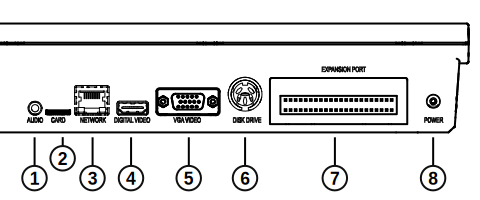
\includegraphics[width=\linewidth]{images/illustrations/mega65-rear.pdf}
\begin{center}
\setlength{\def\arraystretch{1.5}\tabcolsep}{6pt}
\begin{longtable}{ c | l}
	1	& 	3.5mm Audio Jack \\
	2	& 	External microSD Card Slot\\
	3	& 	Network LAN Port \\
	4	& 	Digital Video Connector (including sound) \\
	5	& 	VGA Video Connector \\
	6	& 	IEC Serial Bus Connector for Disk Drives and Printers \\
	7	& 	Cartridge Expansion Port \\
	8	& 	Power Supply Socket \\
\end{longtable}
\end{center}

\vspace{-1cm}

\section{Side Connections}

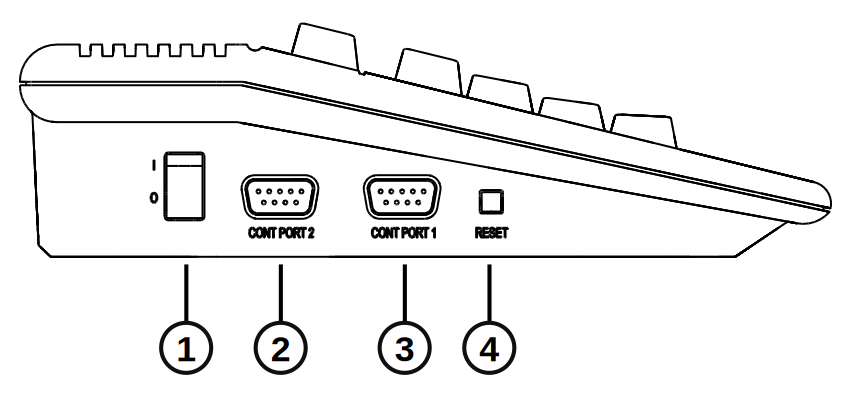
\includegraphics[width=\linewidth]{images/illustrations/mega65-side.pdf}

\begin{center}
\setlength{\def\arraystretch{1.5}\tabcolsep}{6pt}
\begin{longtable}{ c | l}
	1	& 	Power Switch \\
	2	& 	Controller Port 2 \\
	3	& 	Controller Port 1 \\
	4	& 	Reset Button \\
\end{longtable}
\end{center}

Various peripherals can be connected to Controller Ports 1 and 2 such as
joysticks, paddles or mouse devices.

\newpage

\section{MEGA65 Screen and Peripherals}

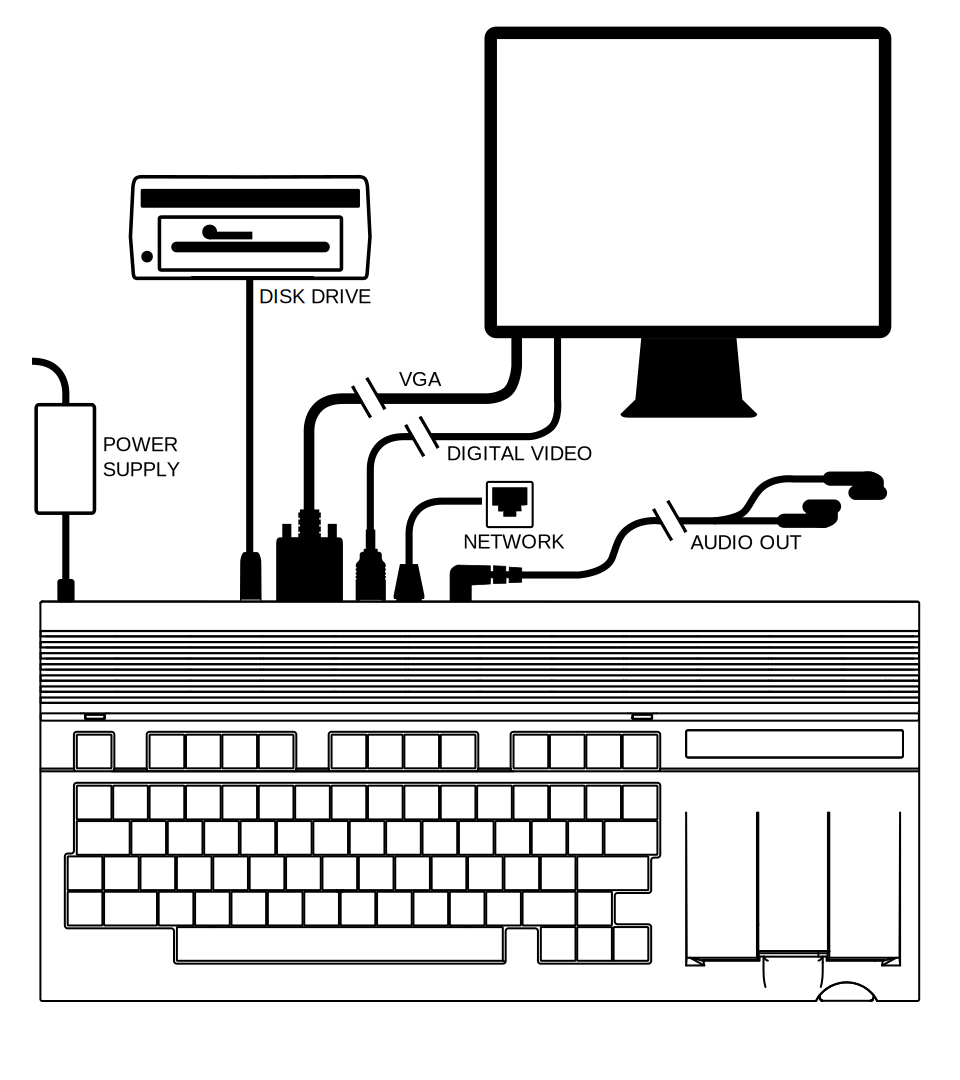
\includegraphics[width=\linewidth]{images/illustrations/mega65-top.pdf}

To connect your MEGA65 to a display:
\index{Display!Connecting}

\begin{enumerate}
	\item Connect the power supply to the power supply socket of the MEGA65.
	\item If you have a VGA monitor and a VGA cable, connect one end to the VGA port of the MEGA65 and the other end into your VGA monitor.
	\item If you have a TV or monitor with a compatible Digital Video connector,\footnote{The Digital Video connector type has a recognizable four-letter commercial name, but the MEGA65 project has not paid the licensing fees to refer to it by this name. This {\em User's Guide} refers to this as the ``Digital Video'' connector.}\index{Digital Video} connect one end of your cable to the Digital Video port of the MEGA65, and the other into the Digital Video port of your monitor. If you own a monitor with a DVI socket, you can use a Digital Video to DVI adapter.
\end{enumerate}

\newpage
\section{Optional Connections}
\index{Disk Drives!Connecting}
\index{Connections!IEC}
\index{SD Cards!Locations}
\begin{enumerate}
	\item The MEGA65 includes an internal 3.5" floppy disk drive. You can also connect older Commodore{\textregistered} IEC serial floppy drives to the MEGA65, such as the Commodore 1541, 1571 or 1581. To use these drives, connect one end of an IEC cable to the Commodore floppy disk drive and the other end to the Disk Drive socket of the MEGA65. You can also connect an SD2IEC device\index{SD2IEC device} or a Pi1541 device.\index{Pi1541 device} With most devices, you can daisy-chain additional floppy disk drives or Commodore compatible printers.
	\item You can connect your MEGA65 to an Ethernet network using a standard Ethernet cable.
	\item For enjoying audio from your MEGA65, you can connect a 3.5mm audio jack cable to an audio amplifier or speaker system. If your system has RCA connectors you will need a 3.5mm audio jack to twin RCA adapter cable. The MEGA65 also has a built-in amplifier to allow the use of headphones.
	\item A microSD card, type SDHC between 4GB and 32GB, can be inserted into the external microSD card slot at the rear of the MEGA65. For more information on using the microSD card slot, see ``Introducing SD Cards'' on page \pageref{sec:introducing-sd-cards}.
	\item Underneath the MEGA65, a small door provides access to the internal SD card and two connectors for future hardware expansion.
\end{enumerate}

\index{Real-Time Clock!Installing the Battery}
\subsection{Installing the Real-Time Clock Battery}

The MEGA65 includes a Real-Time Clock, which is used to display the time and date on the startup screen, to add timestamps to files that the MEGA65 writes to your SD cards, and by the {\bf DT\$}\index{BASIC 65 Variables!DT} and {\bf TI\$}\index{BASIC 65 Variables!TI\$} BASIC65 variables. This clock utilises a CR2032 coin-cell battery\footnote{Early models of MEGA65 with the "R3A" board revision used a battery of type CR1220 for the Real-Time Clock. Revisions "R5" and later, which began shipping in late 2023, use a CR2032 battery.} to keep time when the MEGA65 isn't switched on. The MEGA65 does not include a battery in order to avoid issues related to shipping batteries internationally.

To install the battery, use a Phillips-head screwdriver to open the case, exposing the motherboard.\index{Case!Opening} The case is held together with three screws, all of which are along the bottom of the front side of the case. Once the screws have been removed, carefully lift the top half of the case. Note the orientation of the keyboard connector, then disconnect it.

The battery is located between the controller ports and the keyboard connector.

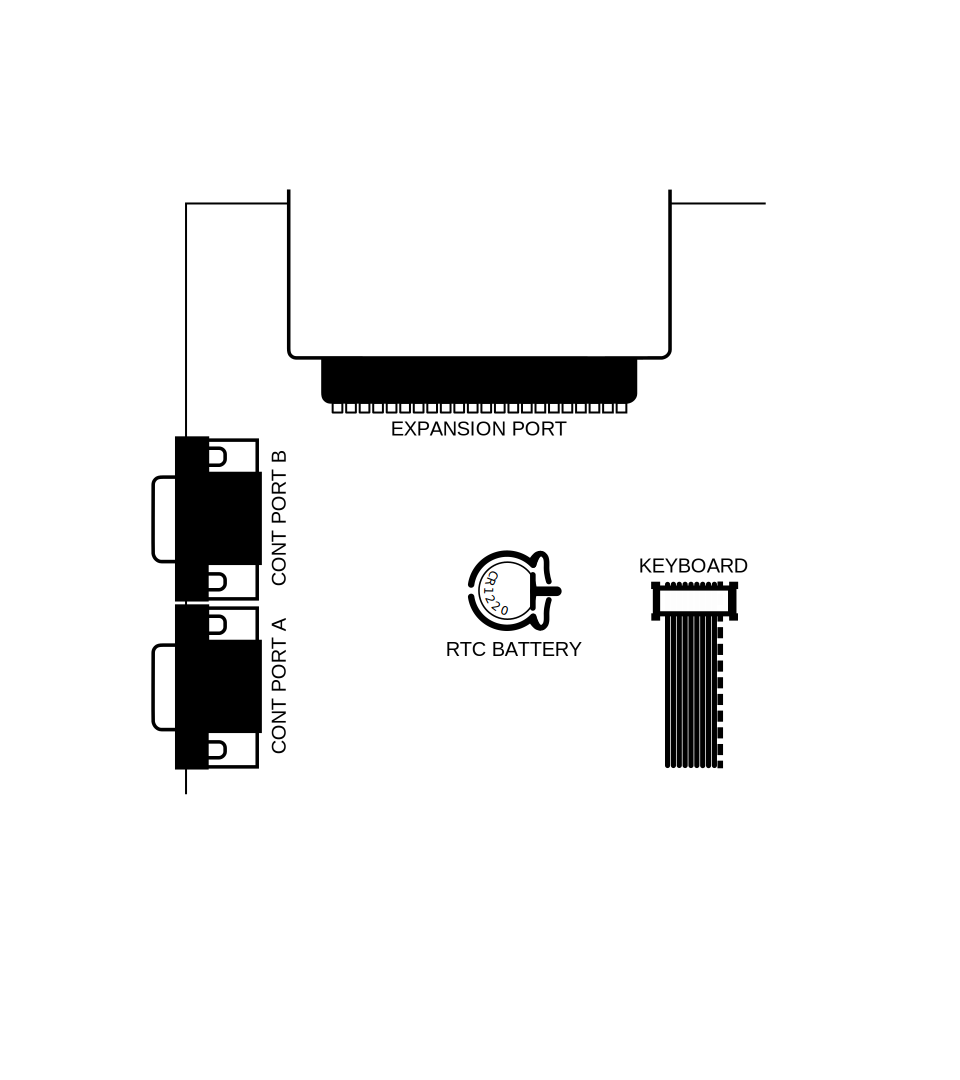
\includegraphics[width=\linewidth]{images/illustrations/rtc-battery-location.pdf}

If you are removing an existing battery, push the battery release lever on the bottom (flat-sided) side of the battery socket away from the battery to remove it. Insert the new battery with the side labelled {\bf +} facing up, and press it into place.

Once you have re-assembled your MEGA65, you can set the time in the Configuration Utility. For more information on how to set the Real-Time Clock, refer to the Configuration Utility section on page \pageref{sec:configuration-utility}.


\newpage

\section{Switching the MEGA65 on for the First Time}
\label{onboarding}

Switch the MEGA65 on using the power switch on the left-hand side of the computer.

When you switch your MEGA65 on for the first time, it displays the initial configuration (``on-boarding'') screen.\index{Configuration!On-boarding} You can use this screen to set the time and date on the Real-Time Clock (if you have installed the CR2032 battery), change the video display mode, and test the audio. All of these settings can be changed later.

\begin{center}
  \includegraphics[width=0.7\linewidth]{images/img011_final_boot_01.png}
\end{center}

For video display modes, you can select between PAL\index{PAL display mode} or NTSC\index{NTSC display mode} emulation, and you can select whether your Digital Video display supports sound. If you are using the VGA video output, the Digital Video sound mode has no effect.

\underline{Note}: A DVI display that does not support sound will not work with the ``enhanced'' sound mode. With such a display, you must select a video mode with ``no sound,'' and connect a speaker to the 3.5 mm audio jack.

PAL and NTSC are analog video signal formats that affect the resolution and vertical sync speed of the video output, even when using a modern digital display. Your display may support either mode, or it may only support one or the other. You can use this screen to test the modes with your display.

Select and test your video configuration. For example, press \specialkey{TAB} to switch to the {\bf PAL 50HZ} mode.
\index{Display!Setting PAL/NTSC}
\begin{center}
  \includegraphics[width=0.7\linewidth]{images/img011_final_boot_02.png}
\end{center}

Press \megakey{SPACE} followed by \megakey{Y} to test the new video mode.

\begin{center}
  \includegraphics[width=0.7\linewidth]{images/img011_final_boot_03.png}
\end{center}

Press \megakey{K} to keep the new video mode.

\begin{center}
  \includegraphics[width=0.7\linewidth]{images/img011_final_boot_04.png}
\end{center}

Take this opportunity to test your sound set-up. Press \megakey{A} to play a sound.

The ``CRT emulation'' option is a fun choice when using a modern flat panel display. It adds vertical gaps between pixels to simulate the CRT raster line. Try it to see if you like it: press the \megakey{C} key to toggle it on and off.

Finally, press \specialkey{RETURN} to complete the configuration.

For more information about configuring your MEGA65, see chapter \vref{cha:configuringyourmega}.

\section{The Intro Disk}
\index{Intro Disk}

After completing the on-boarding configuration, your MEGA65 starts the Intro Disk menu. The Intro Disk is a collection of software made by the MEGA65 community that demonstrates some of the capabilities of the computer. Take some time to browse the menus and try some of the demos. After each demo, press the reset button on the left-hand side of the computer to return to the Intro Disk menu.

\begin{center}
  \includegraphics[width=0.7\linewidth]{images/demo_title.png}
\end{center}

By default, the Intro Disk menu opens each time you switch on the computer. Once you are more familiar with the MEGA65, you may wish to disable this. Press \megakey{D} at the Intro Disk menu to disable its auto-boot feature.\index{Intro Disk!Disabling}

Press \megakey{X} to exit the Intro Disk menu and access BASIC 65. With the Intro Disk auto-boot feature disabled, the MEGA65 goes directly to BASIC 65 when you switch it on.

\begin{center}
  \includegraphics[width=0.7\linewidth]{images/img011_final_boot_06.png}
\end{center}

\section{The Cursor}

The flashing square underneath the \screentext{READY} prompt\index{READY prompt} is called the cursor. The cursor indicates that the computer is ready to accept input. Pressing keys on the keyboard will print their respective characters onto the screen. The characters will be printed at the current cursor position, and the cursor will advance to the next position after every key press.

Here you can type commands, that can do things such as loading a program. You can also start entering program code!

\chapter{Getting Started}
\addtocontents{toc}{\protect\setcounter{tocdepth}{2}}
\hypersetup{bookmarksdepth=5}

\section{Keyboard}
\label{cha:getting-started}
\index{Keyboard}

Now that everything is connected, it's time to get familiar with the MEGA65 keyboard.

You may notice that the keyboard is a little different to the keyboards used on computers today. While most keys will be in familiar positions, there are some specialised keys, and some with special graphic symbols marked on the front.

The graphic symbols are typable in some display modes, similar to letters, numbers, and punctuation. The complete set of characters is known as the {\em PETSCII character set}.\index{PETSCII}

\subsection{Special Keys}

\subsubsection{RETURN}
\index{Keyboard!RETURN}
Pressing \specialkey{RETURN} enters the information you have typed into the MEGA65's memory. The computer will either act on a command, store some information, or display an error message if you made a mistake.

\subsubsection{SHIFT}
\index{Keyboard!Shift Keys}
The two \specialkey{SHIFT} keys are located on the left and the right. They work very much like the Shift key on a regular keyboard. They also perform some special functions as well.

In upper case mode, holding down \specialkey{SHIFT} and pressing any key with two graphic symbols on the front produces the right-hand symbol on that key. For example, \specialkey{SHIFT} and \megakey{J} prints the \graphicsymbol{J} character.

In lower case mode, pressing \specialkey{SHIFT} and a letter key prints the upper case letter on that key.

Finally, holding \specialkey{SHIFT} down and pressing a Function key accesses the function shown on the front of that key. For example: \specialkey{SHIFT} and \megakey{F1} activates \megakey{F2}.


\subsubsection{SHIFT LOCK}
\index{Keyboard!SHIFT LOCK}
In addition to \specialkey{SHIFT} is \specialkey{SHIFT\\LOCK}. Press this key to lock down the Shift function. Now any key you press while \specialkey{SHIFT\\LOCK} is illuminated prints the character to the screen as if you were holding down \specialkey{SHIFT}. This includes special graphic characters.

\subsubsection{CTRL}
\index{Keyboard!CTRL}
\specialkey{CTRL} is the Control key. Holding down \specialkey{CTRL} and pressing another key allows you to perform Control functions. For example, holding down \specialkey{CTRL} and one of the number keys (from \megakey{1} to \megakey{8}) allows you to change text colours. The colour that is printed at the top row on the front of the number key will be used. Holding down \specialkey{CTRL} and pressing \megakey{9} or \megakey{0} switches reverse-text mode on and off.

There are some examples of this on page \pageref{sec:screen-editor}, and all of the Control functions are listed on page \pageref{appendix:controlcodes}.

If a program is being {\bf LIST}ed to the screen, holding down \specialkey{CTRL} slows down the display of each line. You can read more about the {\bf LIST} command on page \pageref{BASIC 65 Commands!LIST}.\index{BASIC 65 Commands!LIST}

Holding \specialkey{CTRL} and pressing \megakey{*} enters the Matrix Mode Debugger (refer to the {\bf MEGA65 Book} for more details).

\subsubsection{RUN STOP}
\index{Keyboard!RUN STOP}
Normally, pressing \specialkey{RUN STOP} stops the execution of a program. Holding \specialkey{SHIFT} while pressing \specialkey{RUN STOP} {\bf RUN}s the first program from disk.\index{BASIC 65 Commands!RUN}

Some programs override the \specialkey{RUN STOP} key and cannot be stopped in this way.

You can boot your MEGA65 into the {\bf Machine Code Monitor}\index{Machine Code Monitor} by holding down \specialkey{RUN STOP} and pressing reset on the left-hand side.

\subsubsection{RESTORE}
\index{Keyboard!RESTORE}
The computer screen can be restored to a clean state without clearing the memory by holding down \specialkey{RUN STOP} and pressing \widekey{RESTORE}. This combination also resets operating system vectors and re-initialises the screen editor, which makes it a handy combination if the computer has become a little confused.

Some programs override the \specialkey{RUN STOP} + \widekey{RESTORE} key combination and cannot be reset in this way.

You can also enter the {\bf Freezer} by pressing and holding \widekey{RESTORE} for half to one second. You can
read more about the Freezer on page \pageref{sec:freezer}.\index{Freezer menu}

\subsubsection{THE CURSOR KEYS}
\index{Keyboard!Cursor Keys}
\nopagebreak
At the bottom right-hand side of the keyboard are the cursor keys. These four directional keys allow you move the cursor to any position for on-screen editing.

The cursor moves in the direction indicated on the keys: \megakey{$\leftarrow$} \megakey{$\uparrow$} \megakey{$\rightarrow$} \megakey{$\downarrow$}.

You don't have to keep pressing a cursor key over and over. If you need to move the cursor a long way, you can keep the key pressed down. When you are finished, simply release the key.

\subsubsection{ARROW KEYS}
\index{Keyboard!Arrow Keys}
These keys are different to the cursor keys! They are \megakeywhite{$\leftarrow$} (next to \megakey{1}), and \megakeywhite{$\uparrow$} (next to \widekey{RESTORE}).
Both arrow keys are used in various BASIC functions and escape sequences.

For example, \megakeywhite{$\leftarrow$} can be used as a shortcut for {\bf SAVE},\index{BASIC 65 Commands!SAVE} and \megakeywhite{$\uparrow$} is used to raise a number to a power (which is the same as multiplying a number by itself a specified number of times).

You can read more about the available escape sequences on page \pageref{escape-sequences}.

These two PETSCII specific keys will always be shown in MEGA65 literature with a white background.

It is also possible to move the cursor up by using \specialkey{SHIFT} and \megakey{$\downarrow$}, and left by using \specialkey{SHIFT} and \megakey{$\rightarrow$}. This owes to the MEGA65's Commodore 64 heritage, which only had two cursor keys.

\subsubsection{INSerT/DELete}
\index{Keyboard!INST DEL}
This is the INSERT / DELETE key. When pressing \specialkey{INST\\DEL}, the character to the left is deleted, and all characters to the right are shifted one position to the left.

To insert a character, hold \specialkey{SHIFT} and press \specialkey{INST\\DEL}. All the characters to the right of the cursor are shifted to the right. This allows you to type a letter, number or any other character at the newly inserted space.


\subsubsection{CLeaR/HOME}
\index{Keyboard!CLR HOME}
Pressing \specialkey{CLR\\HOME} places the cursor at the top left-most position of the screen.

Holding down \specialkey{SHIFT} and pressing \specialkey{CLR\\HOME} clears the entire screen {\it and} places the cursor at the top left-most position of the screen.

If you press \specialkey{CLR\\HOME} accidentally, you can return the cursor to its prior position by pressing \specialkey{ESC} then \specialkey{CLR\\HOME}.

\subsubsection{MEGA KEY}
\index{Keyboard!MEGA Key}
\megasymbolkey or the MEGA key provides a number of different functions and can be used to launch special utilities.

Holding \specialkey{SHIFT} and pressing \megasymbolkey switches between lower and uppercase character modes.

Holding \megasymbolkey and pressing any key with two graphic symbols on the front prints the left-most graphic symbol to the screen. For example,
\megasymbolkey and \megakey{D} prints the \graphicsymbol{d} symbol.

Holding \megasymbolkey and pressing any key that shows a single graphic symbol on the front prints that graphic symbol to the screen.

Holding \megasymbolkey and pressing a number key switches to one of the colours in the second range, i.e., the colour that is printed at the bottom row on the front of the number key will be used.

Holding \megasymbolkey and pressing \specialkey{TAB} enters the Matrix Mode Debugger (refer to the {\bf MEGA65 Book} for more details).

Switching on the MEGA65 or pressing the reset button on the left-hand side while holding down \megasymbolkey switches the MEGA65 into GO64 mode.\index{Commodore 64!GO64 mode}

\subsubsection{NO SCROLL}
\index{Keyboard!NO SCROLL}
If a program is being {\bf LIST}ed to the screen, pressing \specialkey{NO\\SCROLL} pauses the screen output. Press any key to un-pause.

This feature is not available in GO64 mode.\index{Commodore 64!GO64 mode}

\subsubsection{FUNCTION KEYS}
\index{Keyboard!Function Keys}
There are seven Function keys available for use by software applications. \megakey{F1} \megakey{F3} \megakey{F5} \megakey{F7} \megakey{F9} \megakey{F11} and \megakey{F13} can be used to perform special functions.

Hold \specialkey{SHIFT} to access \megakey{F2} through to \megakey{F14} as shown on the front of each Function key.
\index{Keyboard!Shift Keys}
Only Function keys \megakey{F1} to \megakey{F8} are available in GO64 mode.\index{Commodore 64!GO64 mode}

\subsubsection{HELP}
\index{Keyboard!HELP}
\specialkey{HELP} can be used by software and also acts as \megakey{F15} / \megakey{F16}.

\subsubsection{ALT}
\index{Keyboard!ALT}
Holding \specialkey{ALT} down while pressing other keys can be used by software to perform specific functions. This feature is not available in GO64 mode.\index{Commodore 64!GO64 mode}

Holding \specialkey{ALT} down while switching the MEGA65 on activates the Utility Menu.\index{Utility menu} You can format an SD card, or enter the MEGA65 Configuration Utility\index{Configuration!Utility} to select the default video mode and change other settings, or to test your keyboard.

\subsubsection{CAPS LOCK}
\index{Keyboard!CAPS LOCK}
\specialkey{CAPS\\LOCK} works similarly to \specialkey{SHIFT\\LOCK} in C65 and MEGA65-modes, but only modifies the letter keys.

When the MEGA65 is set to run at a reduced processor speed, such as in GO64 mode,\index{Commodore 64!GO64 mode} you can hold down \specialkey{CAPS\\LOCK} to run the processor at full speed temporarily. This is useful in GO64 mode for things such as
speeding up loading from the internal disk drive or SD card, or to greatly speed up the de-packing process after a program is run. MEGA65 mode runs at maximum speed by default.

\addtocontents{toc}{\protect\setcounter{tocdepth}{5}}


\section{The Screen Editor}
\label{sec:screen-editor}

When you switch on your MEGA65 or reset it, the following screen will appear:\footnote{This assumes you have disabled the Intro Disk menu. If the Intro Disk menu is running, press ``X'' to exit to this screen.}

\begin{center}
\includegraphics[width=0.9\linewidth]{images/introduction-screen/layout.png}
\end{center}

The colour bars in the top left-hand side of the screen can be used as a guide to help calibrate the colours of your display. The screen also displays the name of the system, the copyright notice, and the ROM version. The displayed date and time are taken from the internal RTC (Real-Time Clock) at the time the computer was powered on. You can set the date and time in the Configure Utility.

Finally, you will see the \screentext{READY} prompt and the flashing cursor.

You can begin typing keys on the keyboard and the characters will be printed at the cursor position. The cursor itself will advance after each key press.

You can also produce reverse text or colour bars by holding down \specialkey{CTRL} and pressing \megakey{9}, or \megakey{R}. This enters reverse text mode. When this is enabled, you can press and hold the \megakey{Space} bar. While doing so, a white bar will be drawn across the screen.
\index{Keyboard!CTRL}
You can change the current colour by holding \specialkey{CTRL} down and pressing a number key (from \megakey{1}
to \megakey{8}). For example, if you press and hold \specialkey{CTRL} down and press \megakey{1}, the colour will
change to black. Now, when you hold down the \megakey{Space} bar, a black bar will be drawn. If you continue to
change the colour and press the \megakey{Space} bar, you will get an effect similar to the following image:

\begin{center}
\includegraphics[width=0.7\linewidth]{images/introduction-screen/colour-bars.png}
\end{center}

You can disable reverse text mode by holding \specialkey{CTRL} and pressing \megakey{0}.

A further eight colours can be selected by holding down \megasymbolkey and pressing a key from \megakey{1} to \megakey{8}.\index{Keyboard!MEGA Key}

The colour that is printed at the bottom row on the front of the number key will be used. For example, if you held
\megasymbolkey down while pressing \megakey{4}, dark grey will be used. For access to an additional 16 colours of the alternate/rainbow palette, refer to the \specialkey{CTRL} + \megakey{A} shortcut described on page \pageref{appendix:controlcodes}.

\underline{NOTE}:
\begin{itemize}
  \item {\bf Quote Mode}: If you were to press \megakey{"} to open a string, and then try to change
colours, reverse text, move the cursor keys, or use the \specialkey{CLR HOME} key, instead
of these actions instantly occurring, funny PETSCII\index{PETSCII} symbols will appear instead. This is
due to a BASIC facility called {\it quote mode} (described further in the \textbf{MEGA65 Book}),
which allows you to encode such actions into a string so that they can be executed at a later
time (for example, via a {\bf PRINT} statement within your programs). To end {\it quote mode}, simply
type another \megakey{"} to mark the end of your string.
  \item {\bf Insert Mode}: A similar facility is called
{\it insert mode}, where for the number of times you press \specialkey{SHIFT} + \specialkey{INST\\DEL}
to insert a few spaces, the same number of keypresses that follow it will abide by the same
principles of {\it quote mode}.
  \item You can forcefully exit either of these modes by pressing \specialkey{ESC}, \megakey{O}.
\end{itemize}

\needspace{4cm}
You can create fun pictures just by using these colours and letters. Here's an example of what a 4th year student drew:

\begin{center}
\includegraphics[width=0.7\linewidth]{images/caleb-PETSCII-TNT-final}
\end{center}

What will you draw?

\needspace{2cm}
\textbf{Functions}

Functions using \specialkey{CTRL} are called \textbf{Control Codes}.
Functions using \megasymbolkey are called \textbf{Mega Codes}. There are also functions that are called by using \specialkey{SHIFT}, which are called \textbf{Shifted Codes}.

Lastly, \specialkey{ESC} enables the use of \textbf{Escape Sequences}.

You can read about all of these functions in detail on page \pageref{appendix:controlcodes}.

\needspace{2cm}
\textbf{ESC Sequences}

\index{Keyboard!Escape Sequences}
Escape sequences are performed a little differently than a Control function or a Shift function. Instead of holding the modifier key down, an Escape sequence is performed by pressing \specialkey{ESC} and releasing it, followed by pressing the desired key.

For example: to switch between 80 column mode and 40 column mode, press and release \specialkey{ESC}, then press \megakey{X}.

There are more text modes available. You can create flashing text by holding \specialkey{CTRL} down and pressing \megakey{O}. Any characters you type in will flash. Turn flash mode off by pressing \specialkey{ESC}, then \megakey{O}.


\section{Editor Functionality}

The MEGA65 screen editor\index{Screen editor} supports several ways to quickly move the cursor around the screen to help you to be more productive.

For example, press \specialkey{CLR HOME} to go to the home position on the screen. Hold \specialkey{CTRL} down and press \megakey{W} several times. This is the \textbf{Word Advance function}, which jumps your cursor to the next word, or printable character.

You can set custom tab positions on the screen for your convenience. Press \specialkey{CLR HOME} and then \megakey{$\rightarrow$} to move the cursor to the fourth column. Hold down \specialkey{CTRL} and press \megakey{X} to set a tab. Move another 16 positions to the right, and press \specialkey{CTRL} and \megakey{X} again to set a second tab.

Press \specialkey{CLR HOME} to go back to the home position. Hold \specialkey{CTRL} down and press \megakey{I}. This is the \textbf{Forward Tab function}. Your cursor will tab to the fourth position. Press \specialkey{CTRL} and \megakey{I} again. Your cursor will move to position 8. By default, every 8th position is already set as a tabbed position. So the 4th and 20th positions have been added to the existing tab positions. You can continue to press \specialkey{CTRL} and \megakey{I} to advance to the 16th and 20th positions.

\subsection{Creating a Window}
\index{Keyboard!Escape Sequences}
\index{Windows!Escape sequences}

You can set a window on the MEGA65 working screen. Move your cursor to the beginning of the "BASIC 65" text. Press \specialkey{ESC}, then press \megakey{T}. Move the cursor 10 lines down and 15 to the right.

Press \specialkey{ESC}, then \megakey{B}. Anything you type will be contained within this window.

For example, if you were to type \screentext{LIST} to list out a program, the listing will be confined to the window region you have specified:

\begin{center}
\includegraphics[width=0.7\linewidth]{images/set-window.png}
\end{center}

To escape from the window back to the full screen, press \specialkey{CLR HOME} twice.

\subsection{Additional ASCII characters}

You may have noticed a few ASCII characters on the MEGA65 keyboard that aren't traditionally a part of the PETSCII character set.\index{PETSCII} In order to make use of these from within BASIC:

\begin{itemize}
  \item Type either \screentext{FONT A} or \screentext{FONT B}.
  \item Press \megasymbolkey + \specialkey{SHIFT} to switch to lowercase.
\end{itemize}

You will now be able to type those additional ASCII characters via the keyboard. To revert back to the original PETSCII character set, type \screentext{FONT C}.

\subsection{Uppercase and lowercase}

\megasymbolkey + \specialkey{SHIFT} switches between uppercase and lowercase text for the entire display. This works even during program execution, so you can adjust it if a program is in the wrong mode.


\section{The Freezer Menu}
\label{sec:freezer}
\index{Freezer menu}
\nopagebreak
The MEGA65 spends most of its time behaving as a Commodore 65 computer would, either running a program or awaiting instructions in the BASIC environment. Your MEGA65 has additional features that were not part of the original C65 design. You can access many of these features from the Freezer menu.

To open the Freezer menu, hold the \widekey{RESTORE} key for one second, then release it. The MEGA65 will pause whatever it is doing, flicker the border colour, then open the Freezer menu. Whatever program was running remains in memory and can be resumed by pressing the \specialkey{F3} key. You can also abandon the running program and reset the MEGA65 by pressing \specialkey{F5}.

\begin{center}
  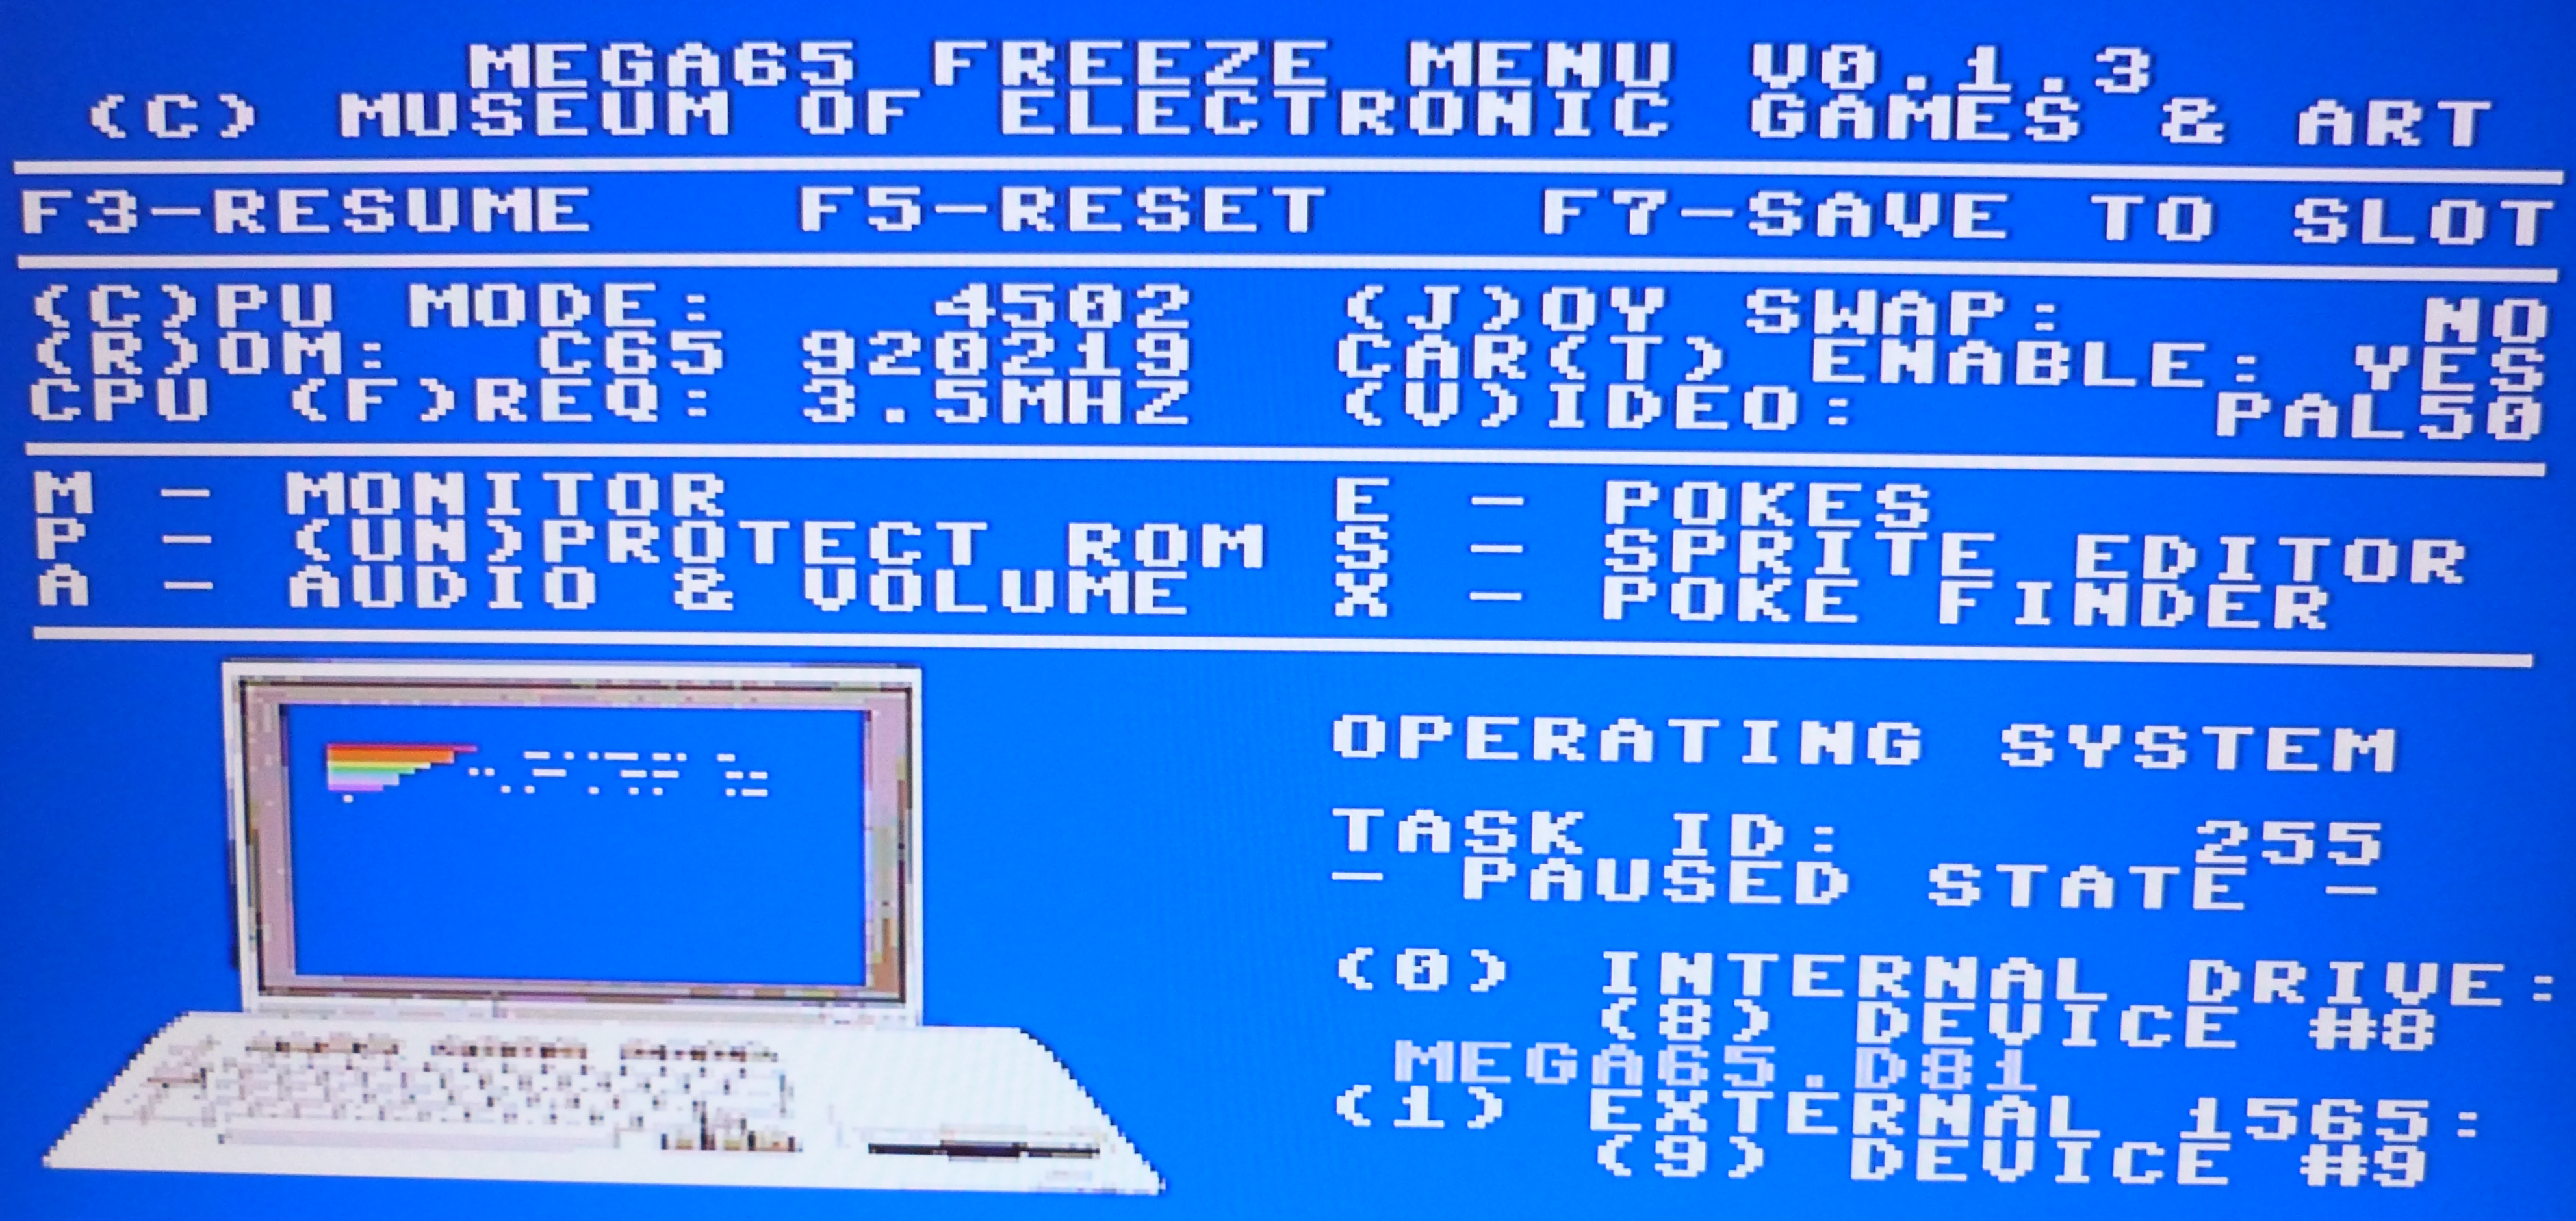
\includegraphics[width=0.7\linewidth]{images/freezer.png}
\end{center}

One feature to remember when playing games is the ``(J)OY SWAP.'' This causes the two joystick ports to trade numbers. If you have a joystick in port 2 and you start a game that expects a joystick in port 1, instead of disconnecting and reconnecting the joystick, open the Freezer menu, press \megakey{J} to swap the port numbers, then resume your game.

This is called the ``Freezer'' menu because the state of the MEGA65 remains frozen while using it. The Freezer menu can store multiple freeze states, and you can switch between them. To save the current state, navigate to an unused {\it freeze slot} using the cursor-right key, then press \megakey{F7}. When the border stops blinking, the state is saved. To restore a state, navigate to the freeze slot, then press \megakey{F3} to resume operation.

The Freezer menu has several built-in options and features. For more information about the MEGA65 Information Utility (``MEGAINFO''), see ``Determining the Versions of Things'' on page \pageref{sec:versions}. For more information about mounting disks and disk images, see chapter \vref{cha:using-disks}.


\section{Running Commodore 64 Software}

The MEGA65 is capable of running Commodore 64 software. There are two ways to do this: the built-in GO64 mode, and the {\it C64 for MEGA65} FPGA core.

\subsection{GO64 Mode}
\index{Commodore 64!GO64 mode}

The original Commodore 65 was designed to be capable of running some Commodore 64 software. The MEGA65 supports this feature, known as ``GO64 mode.''

\underline{NOTE}: Due to how Commodore designed this feature, not all C64 software is compatible with this mode. Unlike the similar feature of the Commodore 128, the Commodore 65 uses a different CPU, and minor differences are known to cause compatibility issues with some software titles.

There are three ways to switch the MEGA65 into GO64 mode:

\begin{itemize}
    \item Switch off the computer, hold the \megasymbolkey and switch it back on.
    \item From the MEGA65 \screentext{READY} prompt, enter this command: \screentext{GO64} Enter \screentext{YES} when prompted.\index{BASIC 65 Commands!GO64}
    \item Switch off the computer, connect a Commodore 64 cartridge to the expansion port, then switch the computer on.
\end{itemize}

\begin{center}
  \includegraphics[width=0.7\linewidth]{images/go64.png}
\end{center}

GO64 mode is actually just a temporary re-configuration of the MEGA65. All of the MEGA65's features are still present, including the Freezer menu for mounting D81 disk images.

Much Commodore 64 software can be found on the Internet in the form of D64 disk images. The MEGA65 only supports D81 disk images via the SD card and Freezer menu. You can use a peripheral such as the SD2IEC\index{SD2IEC device} with the MEGA65's IEC port to use D64 disk images. Be sure to obtain an SD2IEC with an independent power supply, and not one that depends on a Commodore 64 tape connector.\footnote{For more information on SD2IEC devices, see: \url{https://www.c64-wiki.com/wiki/SD2IEC}}

\subsection{The ``C64 for MEGA65'' FPGA Core}
\index{Core!C64 core}\index{Commodore 64!Core}

The {\it C64 for MEGA65} FPGA core by MJoergen and sy2002 re-creates the original Commodore 64 computer on MEGA65 hardware with a high degree of accuracy. It does so by completely replacing the MEGA65 core with one that implements the Commodore 64 chipset, including its CPU. MEGA65 features such as the Freezer menu are not available when running the C64 core. Instead, the core provides its own menu for mounting D64 disk images and other features. Press the \specialkey{HELP} key with the core running to access this menu.

% TODO: When the cartridge-to-core configuration feature is complete:
% With the C64 core installed, you can configure the MEGA65 boot process to use the core when a Commodore 64 cartridge is connected, instead of using the less-compatible GO64 mode. ...
% (Refer to chapter \vref{cha:cores})

For information about installing FPGA cores, see chapter \vref{cha:cores}. To download the {\it C64 for MEGA65} core and read important installation instructions, see: \url{https://github.com/MJoergen/C64MEGA65}

\section{The Screen Editor}
\label{sec:screen-editor}

When you switch on your MEGA65 or reset it, the following screen will appear:

\begin{center}
\includegraphics[width={10cm}]{images/introduction-screen/layout.png}
\end{center}

The colour bars in the top left-hand side of the screen can be used
as a guide to help calibrate the colours of your display.
The screen also displays the name of the system,
the copyright notice, and the ROM version.
The displayed date and time are taken from the internal RTC
(Real-Time Clock), which can be set in the Configure Menu.

Finally, you will see the \screentext{READY} prompt and the flashing cursor.

You can begin typing keys on the keyboard and the characters will be
printed at the cursor position. The cursor itself will advance after
each key press.

You can also produce reverse text or colour bars by holding down \specialkey{CTRL} and pressing \megakey{9}, or \megakey{R}. This enters reverse text mode. When this is enabled, you can press and hold the \megakey{Space} bar. While doing so, a white bar will be drawn across the screen.
\index{Keyboard!CTRL}
You can even change the current colour by holding \specialkey{CTRL} down and pressing a number key (from \megakey{1} to \megakey{8}). For example, if you press and hold \specialkey{CTRL} down and press \megakey{1}, the colour will change to black. Now, when you hold down the \megakey{Space} bar, a black bar will be drawn. If you continue to change the colour and press the \megakey{Space} bar, you will get an effect similar to the image below:


\begin{center}
\includegraphics[width={10cm}]{images/introduction-screen/colour-bars.png}
\end{center}


\index{Keyboard!MEGA Key}
You can disable reverse text mode by holding \specialkey{CTRL} and pressing \megakey{0}.

By pressing any key, characters will be printed to the screen in the chosen colour.

A further eight colours can be selected by holding down \megasymbolkey and pressing a key from \megakey{1} to \megakey{8}.
The colour that is printed at the bottom row on the front of the number key will be used. For example, if you held
\megasymbolkey down while pressing \megakey{4}, dark gray will be used. For even more colours, see \bookvref{appendix:escape-colours}.

\needspace{4cm}
You can create fun pictures just by using these colours and letters.  Here's an example of what a year four student drew:

\begin{center}
\includegraphics[width={6cm}]{images/caleb-PETSCII-TNT-final}
\end{center}

What will you draw?

\needspace{2cm}
\textbf{Functions}

Functions using \specialkey{CTRL} are called \textbf{Control Codes}.
Functions using \megasymbolkey are called \textbf{Mega Codes}. There are also functions that are called by using \specialkey{SHIFT}, which
are called \textbf{Shifted Codes}.

Lastly, \specialkey{ESC} enables the use of \textbf{Escape Sequences}.

You can read about all of these functions in detail in \bookvref{appendix:controlcodes}, but some are shown in this section.


\needspace{2cm}
\textbf{ESC Sequences}
\index{Keyboard!Escape Sequences}
Escape sequences are performed a little differently than a Control function or a Shift function. Instead of holding the modifier key down, an Escape sequence is performed by pressing \specialkey{ESC} and releasing it, followed by pressing the desired key code.

For example: to switch between 40/80 column mode, press and release \specialkey{ESC}, then press \megakey{X}.

There are more modes available. You can create flashing text by holding \specialkey{CTRL} down and pressing \megakey{O}. Any characters you type in will flash. Turn flash mode off by pressing \specialkey{ESC},  then \megakey{O}.



\section{Editor Functionality}


The MEGA65 screen can allow you to do advanced tabbing, and quickly move around the screen in many ways to help you to be more productive.

For example, press \specialkey{CLR HOME} to go to the home position on the screen. Hold \specialkey{CTRL} down and press \megakey{W} several times. This is the \textbf{Word Advance function}, which jumps your cursor to the next word, or printable character.

You can set custom tab positions on the screen for your convenience. Press \specialkey{CLR HOME} and then \megakey{$\rightarrow$} to the fourth column. Hold down \specialkey{CTRL} and press \megakey{X} to set a tab. Move another 16 positions to the right again, and press \specialkey{CTRL} and \megakey{X} again to set a second tab.

Press \specialkey{CLR HOME} to go back to the home position. Hold \specialkey{CTRL} down and press \megakey{I}. This is the \textbf{Forward Tab function}. Your cursor will tab to the fourth position. Press \specialkey{CTRL} and \megakey{I} again. Your cursor will move to position 8. Why do you ask? By default, every 8th position is already set as a tabbed position. So the 4th and 20th positions have been added to the existing tab positions. You can continue to press \specialkey{CTRL} and \megakey{I} to advance to the 16th and 20th positions.

To find the complete set of Control codes, see \bookvref{appendix:controlcodes}.

\textbf{Creating a Window}

You can set a window on the MEGA65 working screen. Move your cursor to the beginning of the "BASIC 65" text. Press \specialkey{ESC}, then press \megakey{T}. Move the cursor 10 lines down and 15 to the right.

Press \specialkey{ESC}, then \megakey{B}. Anything you type will be contained within this window.

To escape from the window back to the full screen, press \specialkey{CLR HOME} twice.


\textbf{Extras}

Long press on \widekey{RESTORE} to go into the Freeze Menu.  Then press \megakey{J} to switch joystick ports without having to physically swap the joystick to the other port.

Go to \textbf{Fast mode} (40.5MHz) by either typing \screentext{FAST}, or \screentext{POKE 0,65} or use the Freeze Menu.

Return back to \textbf{Slow mode} (1MHz) by either typing \screentext{FAST 1}, or \screentext{POKE 0,64} or use the Freeze Menu.

\megasymbolkey + \specialkey{SHIFT} switches between uppercase and lowercase text for the entire display.


\part{FIRST STEPS IN CODING}

\chapter{How Computers Work}

Did you know that many computer experts and programmers learned how to
use computers when they were still small children?
Home computers only became common in the early 1980s. They were so new,
that people would often write programmes to do
what they wanted to do, because no software existed to do the job for them.

It was also quite common for people working in all
sorts of office jobs to learn how to program the computers they used for
their jobs.  For example, the people processing payroll
for a company would often learn how to program the computer to calculate
the everyone's pay!

Things have changed a lot since then, though.
Now most people choose existing programmes or apps to do what they need,
and think that programming is a specialised skill that only some people
have the ability to learn.
But this isn't true.  Of course, like every other field of pursuit
everyone will be better at some things than others,
whether it be sports, knitting, maths or writing. But almost
everyone is able to learn enough to help them in their life.

We created the MEGA65, because we believe that YOU can learn to
programme, so that computers can be more useful to you, and as with
learning any new skill, that you can have the satisfaction and enjoyment
and new adventures that this brings!


\phantomsection
\section{Computers are stupid. Really stupid}

How can this be so? Computers are able to do so many different things, often thousands of times faster than a person can.
So how can we say that computers are stupid?  The answer is that no computer can do anything that it hasn't been instructed
by a person to do.  Even the latest Artificial Intelligence systems were instructed how to learn (or how to learn, how to learn).
To understand why this is so, it is helpful to understand how computers really work.

\subsection{Making an Egg Cup Computer}

The heart of a computer is its Central Processing Unit, or CPU for short.  Many modern computers have more than one CPU, but let's keep
things simple to begin with.  The CPU has a set of simple instructions that it understands, like, ``get the thing from cup \#21,'' ``put this thing into cup \#403,'' ``add these things together,'' or ``do the following instruction, but only if the thing in cup \#712 is the number 3.''

But what do we mean with all of these ``things'' and ``cups''? Let's start by thinking about how we could pretend to be a computer using
just an empty egg carton, some small pieces of paper and a pencil or pen.  Start by writing numbers, beginning with one, in each of the
little egg cups in the egg carton.  Then write the number zero on a little scrap of paper and put it in the first cup.  Do the same for the other cups. You should now have an egg carton with numbered cups, and with every cup having a scrap of paper with the number zero written on it. Now we just need to decide on a few simple rules that will explain how our egg-cup computer will work:

\begin{itemize}
  \item First, each cup is allowed to hold exactly one thing at a time. Never more. Never less.  This so that when we ask the question ``what is in box such-and-such,'' that there is a single clear answer. It's also how computer memory works: Each piece of memory can hold only one thing at a time.

  \item Second, we need a way for the computer to know what to do next. On most computers this is called the Programme Counter, or PC, for short (not to be confused with PC when people are talking about a Personal Computer).  The PC is just the number of the next of the next memory location (or in our case, egg-cup), that the computer will examine, when deciding what to do next.  You might like to have another piece of paper that you can use to write the PC number on as you go along.

  \item Third, we need to have a list of things that the egg-cup computer will do, based on what number is in the egg-cup indicated by the 
    PC.
\end{itemize}

So let's come up with the set of things that the computer can do, based on the number in the egg-cup indicated by the PC.  We'll keep things simple with just the following:

\begin{center}
  \begin{longtable}{|R{2.2cm}|p{8cm}|}

    \hline
        {\textbf{Number in the egg-cup}} & {\textbf{Action}} \\ \hhline{|=|=|}
        0 & {i) Add one to the PC, and do nothing else.} \\ \hline
        1 & {i) Add one to the PC. \hfill\break ii) Set the PC to be the number stored in that egg-cup.} \\ \hline
        2 & {i) Add one to the PC. \hfill\break ii) Add the number in the egg-cup indicated by the PC to the number in the egg-cup indicated by the number in the egg-cup following that. \hfill\break iii) Put the answer in the egg-cup indicated by the egg-cup following that. \hfill\break iv) Finally, add two more to the PC, to skip over the egg-cups that we made use of.}  \\ \hline
  \end{longtable}
\end{center}

Don't worry if that sounds a bit confusing for now, specially that last one -- we will go through it in detail very soon!
The best way to explain it, is to go through some examples.


\chapter{Getting Started in BASIC}
\label{cha:basic-getting-started}

It is possible to code on the MEGA65 in many languages,
however most people start with BASIC.  That makes sense,
because BASIC stands for Beginner's All-purpose Symbolic
Instruction Code: It was made for people like you to get
started with in the world of coding!

A few short words before we dive in: BASIC is a programming
language, and like spoken language it has conventions, grammar
and vocabulory.  Fortunately, it is much quicker and easier
to learn than our complex human languages. But if you pay
attention, you might notice some of these stuctures, and that
can help you along your path in the world of coding.

If you haven't already read Chapter \ref{cha:getting-started},
it might be a good idea to do so. This will help you be able to
more confidently interact with the MEGA65 computer.

It's also great to remember that if you really confuse the MEGA65,
you can always get back to the READY. prompt by just pressing the
reset button on the left-hand side of the keyboard, or if that
doesn't help, then by turning it off
and on again using the power switch on the left-hand side of the keyboad.
You don't have to worry about shutting the computer
down properly or any of that nonsence.  The only thing to remember
is that if you had any unsaved work, it will be lost when you turn
the computer off and on again or press the reset button.

Finally, if you don't understand all of the descriptions and information
with an example -- don't worry! We have provided as much information
as we can, so that it is there in case you have questions, encounter problems are are
just curious to discover more.  Feel free to skip ahead to the examples
and try thing out, and then you can go back and re-read it when you are motivated
to find something out, or help you work though a problem.  And if you don't find
the answer to your problem, send us a message!  There are support forums for the
MEGA65 at \url{https://mega65.net}{https://mega65.net}, and you can
report problems with this guide at:

\url{https://github.com/mega65/mega65-user-guide}{https://github.com/mega65/mega65-user-guide}

We hope you have as much fun learning to programme the MEGA65 as
we have had making it!

\section{Your first BASIC programmes}

The MEGA65 was designed to be programmed! When you turn it on,
it takes a couple of seconds to get its house in order, and then
it quickly shows you a ``READY.'' prompt and flashing block called
the cursor.  When the cursor is blinking, it tells you that the
computer is waiting for input.  The ``READY.'' message tells you
that the BASIC programming language is running and ready for you to
start programming.  You don't even need to load any programmes --
you can just get started.

Try typing the following into the computer and see what happens:

\begin{tcolorbox}[colback=black,coltext=white]
\verbatimfont{\codefont}
\begin{verbatim}
HELLO COMPUTER
\end{verbatim}
\end{tcolorbox}

To do this, just type the letters as you see them above.  The computer
will already be in upper-case mode, so you don't need to hold the \specialkey{SHIFT}
or \specialkey{CAPS\\LOCK}} key down.  When you have typed ``HELLO COMPUTER'' press
  the \specialkey{RETURN} key.  This tells the computer you want it to accept the
  line of input you have typed.  When you do this, you should see a message something
  like the following:

  If you saw a \screentext{SYNTAX ERROR} message something like that one, then congratulations:
  You have succeeded in communicating with the computer!
  Error messages sound much nastier than they are.  The MEGA65 uses them, especially
  the syntax error to tell you when it is having trouble understanding what you have
  typed, or what you have put in a programme.  They are nothing to be afraid of, and
  experienced programmers get them all the time.

  In this case, the computer was confused because it doesn't understand the word
  ``hello'' or the word ``computer''.  That is, it didn't know what you wanted it to
  do.  In this regard, computers are quite stupid. They know only a few words, and
  aren't particularly imaginative about how the interpret them.

  So let's try that again in a way that the computer will understand.  Try typing
  the following in.  You can just type it right away. It doesn't matter that the
  syntax error message can still be seen on the screen.  The compute has already
  forgotten about that by the time it told you \screentext{READY.} again.

\begin{tcolorbox}[colback=black,coltext=white]
\verbatimfont{\codefont}
\begin{verbatim}
PRINT "HELLO COMPUTER"
\end{verbatim}
\end{tcolorbox}

Again, make sure you don't use shift or shift-lock while typing it in.  The symbols around
the words \screentext{HELLO COMPUTER} are double-quotes.  If you are used to an Australian or American
keyboard, you might discover that they double-quote key is in a rather different place to
where you are used to:  Double-quotes can be typed on the MEGA65 by holding down the
\specialkey{SHIFT} key, and then pressing 2.  Don't forget to press the \specialkey{RETURN}
key when you are done, so that the computer knows you want it to do something with your input.

If you make a mistake while typing, you can use the \specialkey{INST\\DEL} to rub out the mistake
and fix it up.  You can also use the cursor keys to move back and forth on the line while
you edit the line you are typing, but there is a bit of a trick if you have already typed
a double-quote: If you try to use the cursor keys, it will print a funny reversed symbol
instead of moving the cursor.  This is because the computer thinks you want to record
moving the cursor in the text itself, which can be really useful and fun, and which you can
read more about in Chapter \ref{cha:getting-started}. But for now, if you
make a mistake just press the \specialkey{RETURN} key and type the messed up line again.
Hopefully now you will see something like the following:

\setlength{\intextsep}{0pt}%
  \begin{wrapfigure}{i}{0.6\linewidth}
    \includegraphics[width=\linewidth]{images/print-hello-computer.png}
  \end{wrapfigure}

  This time no new \screentext{SYNTAX ERROR} message should appear. But if some kind
  of error message has appeared, just try typing in the command again, after
  taking a close look to work out where the mistake might be.

  Instead of an error, we should see \screentext{HELLO COMPUTER} repeated underneath
  the line you typed in.  The reason this happened is that the computer
  does undestand the word \screentext{PRINT}.  It knows that whatever comes after
  the word \screentext{PRINT} should be printed to the screen.  We had to put \screentext{HELLO
  COMPUTER} inside double-quotes to tell the compute that we want it to be
  printed literally.

  If we hadn't put the double-quotes in, the computer would have thought
  that \screentext{HELLO COMPUTER} was the name of a stored piece of information.
  You can try it, if you like.

  \begin{wrapfigure}{i}{0.6\linewidth}
    \includegraphics[width=\linewidth]{images/print-hello-computer-no-quotes.png}
  \end{wrapfigure}  

  But because we haven't stored any piece of information in such a place,
  the computer will have zero there, so the computer will print the number
  zero, like this. If the computer prints zero or some other number when
  you expected a message of some sort, this can be the reason.

  In the above examples we typed commands in directly, and the computer executed
  them immediately after you pressed the \specialkey{RETURN} key.  This is why
  typing commands in this way is often called {\em direct mode} or {\em immediate mode}.
  
  But we can also tell the computer to remember a list of commands to execute one
  after the other.   This is done using the rather unimaginatively named {\em non-direct mode}.
  To use non-direct mode, we just put a number between 0 and 63999 at the start of
  the command.  The computer will then remember that command.  Unlike when we executed
  a direct-mode command, the computer doesn't print \screentext{READY.} again. Instead the cursor
  just reappears on the next line, ready for us to type in more commands.

  Let's try that out with a simple little programme.  Type in the following three lines of
  input:

\begin{tcolorbox}[colback=black,coltext=white]
\verbatimfont{\codefont}
\begin{verbatim}
1 FOR I = 1 TO 10 STEP 1
2 PRINT I
3 NEXT I
\end{verbatim}
\end{tcolorbox}

When you have done this, the screen should show something like this:

\setlength{\intextsep}{0pt}%
  \begin{wrapfigure}{i}{0.6\linewidth}
    \includegraphics[width=\linewidth]{images/first-steps-for-loop-programme-1.png}
  \end{wrapfigure}

If it doesn't you
can try again. Don't forget, if you feel that the computer is getting all muddled up,
you can just press the reset button or flip the power switch off and on on the left side of the
computer to reboot it. This only takes a couple of seconds, and doesn't hurt the MEGA65
in anyway.

We have told the computer to remember three commands, that is, \screentext{FOR I = 1 TO 10 STEP 1},
\screentext{PRINT I}
and \screentext{NEXT I}.  We have also told the computer which order we would like to run them in: The
computer will start with the command with the lowest number, and execute each command that
has the next higher number in turn, until it reaches the end of the list.  So it's a bit like
a reminder list for the computer. This is what we call a programmme, a bit like the progamme at
a concert or the theatre, it tells us what is coming up, and in what order.
So let's tell the computer to execute this programme.

But first, let's try to guess what will happen.  Let's start with the middle command, \screentext{PRINT I}.
We've seen the \screentext{PRINT} command, and we know it tells the computer to print things to the screen.
The thing it will try to print is \screentext{I}.  Just like before, because there are no double-quotes
around the \screentext{I}, it will try to print a piece of stored information.  The piece of information
it will try to print will be the piece associated with the thing \screentext{I}.

When we give a piece of
information like this a name, we call it a {\em variable}\idx{variable}.  They are called
variables because they can vary.  That is, we can replace the piece of information associated
with the variable called I with another piece of information.  The old piece will be forgotten
as a result.  So if we gave a command like \screentext{LET I = 3}, this would replace whatever was stored
in the variable called \screentext{I} with the number 3.

Back to our programme, we now know that the 2\textsuperrscript{nd} command will try to print the piece of information
stoed in the variable \screentext{I}.  So lets look at the first command: \screentext{FOR I = 1 TO 10 STEP 1}.  Although
we haven't seen the \screentext{FOR} command before, we can take a bit of a guess at how it works. It looks like
it is going to put something into the variable \screentext{I}.  That something seems to have something to do
with the range of number 1 through 10, and a step or interval of 1.  What do you think it will do?

If you guessed
that it will put the values 1, 2, 3, 4, 5, 6, 7, 8, 9 and then 10 into the variable \screentext{I}, then you
can give yourself a pat on the back, because that's exactly what it does.  It also helps us to
understand the 3\textsuperscript{rd} command, \screentext{NEXT I}: That command tells the computer to put the next value into
the variable \screentext{I}.  And here is a little bit of magic: When the computer does that, it goes back
up the list of commands, and continues again from the command after the \screentext{FOR} command.

So lets pull that together: When the computer executes the first command, it discovers that it has
to put 10 different values into the variable \screentext{I}. It starts by putting the first value in there, which
in this case will be the number 1.
The computer then continues to the second command, which tells the computer to print the piece of
information that is currently stored in the variable called \screentext{I}. That will be the number 1, since
that was the last thing the computer was told to put there.  Then the computer proceeds to the
third command, which tells it that it is time to put the next value into the variable \screentext{I}.  So the
computer will throw away the number 1 that is curently in the variable \screentext{I}, and put the number 2 in
there, since that is the next number in the list.  It will then continue from the 2\textsuperscript{nd} command,
which will cause the computer to print out the contents of the variable \screentext{I} again.  Except that this
time \screentext{I} has had the number 2 stored in it most recently, so the computer will print the number 2.
This process will repeat, until the computer has printed all ten values that the \screentext{FOR} command
indicated it to do.   

To see this in action, we need to tell the computer to execute the programme of commands we typed in.
We do this by using the \screentext{RUN} command. Because we want it to run the programme immediately, we
should use immediate mode (remember, this is another name for direct mode).
So just type in the word \screentext{RUN} and press the \specialkey{RETURN} key.  You should then see a display
that looks something like the following:

\pagebreak

\setlength{\intextsep}{0pt}%
  \begin{wrapfigure}{i}{0.6\linewidth}
    \includegraphics[width=\linewidth]{images/first-steps-for-loop-programme-1-running.png}
  \end{wrapfigure}

  You might notice a couple of things here:

  First, the computer has told us it is \screentext{READY.} again
  as soon as it finished running the programme. This just makes it easier for us to know when we
  can start giving commands to the computer again.

  Second, when the computer got to the bottom of the screen
  it automatically scrolled the display up to make space.  This is quite normal.  What is important
  to remember, is that the computer forgets everything that scrolls off the top.  The only exception
  is if you have told the computer to remember a command by putting a number in front of it.  So
  our programme is quite safe for now. We can see that this is the case by typing the \screentext{RUN} command a
  couple more times: The programme listing will have scrolled off the top of the screen, but we can
  still RUN the programme, because the computer has remembered it.  Give it a try!

  \subsubsection{Exercises to try}

  \subsubsubsection{Can you make it count to a higher or lower number?}

  At the moment it counts from 1 to 10.  Can you change it to count to 20 instead?  Or to count from 3 to 17?
  
  (a) make it count  to a larger or smaller number
 (b) increase by a different amount each iteration
 (c) print out one of the times tables
(d) print out all of the times tables from 1x1 to 10x10


  
  
  
\section{First steps with text and numbers}

\section{Making simple decisions}

\section{Random numbers and chance}

\input{morebasic}
\input{datainbasic}

\part{SOUND AND GRAPHICS}


\newcommand{\blkb}{\cellcolor[rgb]{0,0,0}\textcolor{white} 0 }
\newcommand{\bwn}{\cellcolor[rgb]{.26,.22,0}\textcolor{white} 9 }
\newcommand{\ora}{\cellcolor[rgb]{.44,.31,.15}8 }
\newcommand{\red}{\cellcolor[rgb]{.6,.4,.35}A }
\newcommand{\lgr}{\cellcolor[rgb]{.58,.58,.58}F }
\newcommand{\yel}{\cellcolor[rgb]{.72,.78,.44}7 }

\newcommand{\redb}{\cellcolor[rgb]{.6,.4,.35} 1 }

\chapter{Graphics}
\label{cha:graphics}

Let's have some fun with graphics!
In this part of the book, we want to examine the MEGA65's graphics modes by walking through example code in machine language and BASIC to get to know the various options of the MEGA65 in the area of graphics. First of all, it is important to know that the MEGA65 supports three different basic graphics modes:

\begin{itemize}
	\item Bitmap graphics
	\item Graphics based on character sets
	\item Bitplanes
\end{itemize}


\section*{Bitmap Graphics}

In bitmap graphics every pixel of a graphic is stored separately. The way the pixels are hold in memory varies from system to system and in most cases depends on the performance of the hardware. If memory would be unlimited, the easiest way to remember a pixel is to save its RGB-values in three separate bytes. Example: 0xFFFFFF for white would result in three values to be stored: \$FF, \$FF and \$FF. To be honest, this is too simple and not really efficient. Let’s think about another way. Why not defining a color table (or color palette) and store the RGB values once and finally only reference the color by its index in the table? This will save us a lot of memory! Let's imagine we would create a colorful 8x8 bitmap to represent an "A" on the screen. Colourful means, we want it in some brownish colors. The color table for it may look like this:

\begin{center}
\begin{tabular}{|l|l|}
\hline
	Index & Color \\
\hline
	\blkb & Black \\
	\bwn & Brown \\
	\ora & Orange \\
	\red & Light Red \\
	\lgr & Light Grey \\
	\yel & Yellow \\
\hline
\end{tabular}
\end{center}

The color values, by the way, are exactly the same as the color values from the standard C64 color palette. Next we design the "A". Each pixel references a value from the color table above.


\begin{center}
\begin{tabular}{|m{6pt}|m{6pt}m{6pt}m{6pt}m{6pt}m{6pt}m{5pt}m{6pt}m{6pt}|}
\hline
	& 7 & 6 & 5 & 4 & 3 & 2 & 1 & 0 \\
\hline
	0 & \blkb & \blkb & \blkb & \blkb & \blkb & \blkb & \blkb & \blkb \\
	1 & \red & \lgr & \yel & \lgr & \red & \ora & \blkb & \blkb \\
	2 & \lgr & \lgr & \blkb & \blkb & \ora & \red & \blkb & \blkb \\
	3 & \yel & \yel & \blkb & \blkb & \ora & \red & \blkb & \blkb \\
	4 & \yel & \lgr & \lgr & \red & \red & \red & \blkb & \blkb \\
	5 & \lgr & \red & \blkb & \blkb & \ora & \red & \blkb & \blkb \\
	6 & \red & \red & \blkb & \blkb & \red & \red & \blkb & \blkb \\
	7 & \ora & \bwn & \blkb & \blkb & \ora & \red & \blkb & \blkb \\
\hline
\end{tabular}
\end{center}

But how much memory does this little graphic use?

If we create an one-dimensional array, we will get an array with 64 elements, because our graphic consists of 8x8 pixels = 64 color values that have to be saved. If we transfer that to the memory of the MEGA65, it means that we have 64 bytes to store in memory. However, full-screen graphics are made up of far more pixels. On the C64 and of course also on the MEGA65, 320x200 pixels are required to generate a graphic that fills the entire screen. If we transfer this to our array, we would have a total of 64,000 entries. Converted to the memory of the MEGA65, that is 64,000 bytes or nearly 64 kilobytes of data! If we now also consider that the good old C64 only had 64K of RAM available, we recognize the Drama! That's just too much data! We need strategies to reduce our bitmap data. On the C64 we had two types of bitmap graphics and both come with its own concepts to use as less memory as possible.

\begin{itemize}
	\item Hires
	\item Multicolor (MCM)
\end{itemize}


\subsection*{Hires}

First, a bitmap is divided into blocks of 8x8 pixels each. In order to achieve the full resolution of 320x200 pixels, 40 of such blocks next to each other builds up a line. If we now build up 25 lines, we arrive at a graphic that fills the complete screen.

\begin{adjustbox}{width=\textwidth,center}
\begin{footnotesize}
\begin{tabular}[h]{|C{10pt}|C{5pt}|C{5pt}|C{5pt}|C{5pt}|C{5pt}|C{5pt}|C{5pt}|C{5pt}|C{5pt}|C{5pt}|C{5pt}|C{5pt}|C{5pt}|C{5pt}|C{5pt}|C{5pt}|C{5pt}|C{5pt}|C{5pt}|C{5pt}|C{5pt}|C{5pt}|C{5pt}|C{5pt}|C{5pt}|C{5pt}|C{5pt}|C{5pt}|C{5pt}|C{5pt}|C{5pt}|C{5pt}|C{5pt}|C{5pt}|C{5pt}|C{5pt}|C{5pt}|C{5pt}|C{5pt}|C{5pt}|}
\hline
  &   &   &  &  &  &   &   &   &   & 1  & 1  & 1  & 1  & 1  & 1  & 1  & 1  & 1  & 1  & 2  & 2  & 2  & 2  & 2  & 2  & 2  & 2  & 2  & 2  & 3  & 3  & 3  & 3  & 3  & 3  & 3  & 3  & 3  & 3  & 4  \\
  & 1 & 2 & 3& 4& 5& 6 & 7 & 8 & 9 &  0 & 1  &  2 &  3 &  4 &  5 &  6 &  7 &  8 &  9 &  0 &  1 &  2 &  3 &  4 &  5 &  6 &  7 &  8 &  9 &  0 &  1 &  2 &  3 &  4 &  5 &  6 &  7 &  8 &  9 &  0 \\
\hline
   1 & & & & & & & & & & & & & & & & & & & & & & & & & & & & & & & & & & & & & & & & \\\hline
   2 & & & & & & & & & & & & & & & & & & & & & & & & & & & & & & & & & & & & & & & & \\\hline
   3 & & & & & & & & & & & & & & & & & & & & & & & & & & & & & & & & & & & & & & & & \\\hline
   4 & & & & & & & & & & & & & & & & & & & & & & & & & & & & & & & & & & & & & & & & \\\hline
   5 & & & & & & & & & & & & & & & & & & & & & & & & & & & & & & & & & & & & & & & & \\\hline
   6 & & & & & & & & & & & & & & & & & & & & & & & & & & & & & & & & & & & & & & & & \\\hline
   7 & & & & & & & & & & & & & & & & & & & & & & & & & & & & & & & & & & & & & & & & \\\hline
   8 & & & & & & & & & & & & & & & & & & & & & & & & & & & & & & & & & & & & & & & & \\\hline
   9 & & & & & & & & & & & & & & & & & & & & & & & & & & & & & & & & & & & & & & & & \\\hline
  10 & & & & & & & & & & & & & & & & & & & & & & & & & & & & & & & & & & & & & & & & \\\hline
  11 & & & & & & & & & & & & & & & & & & & & & & & & & & & & & & & & & & & & & & & & \\\hline
  12 & & & & & & & & & & & & & & & & & & & & & & & & & & & & & & & & & & & & & & & & \\\hline
  13 & & & & & & & & & & & & & & & & & & & & & & & & & & & & & & & & & & & & & & & & \\\hline
  14 & & & & & & & & & & & & & & & & & & & & & & & & & & & & & & & & & & & & & & & & \\\hline
  15 & & & & & & & & & & & & & & & & & & & & & & & & & & & & & & & & & & & & & & & & \\\hline
  16 & & & & & & & & & & & & & & & & & & & & & & & & & & & & & & & & & & & & & & & & \\\hline
  17 & & & & & & & & & & & & & & & & & & & & & & & & & & & & & & & & & & & & & & & & \\\hline
  18 & & & & & & & & & & & & & & & & & & & & & & & & & & & & & & & & & & & & & & & & \\\hline
  19 & & & & & & & & & & & & & & & & & & & & & & & & & & & & & & & & & & & & & & & & \\\hline
  20 & & & & & & & & & & & & & & & & & & & & & & & & & & & & & & & & & & & & & & & & \\\hline
  21 & & & & & & & & & & & & & & & & & & & & & & & & & & & & & & & & & & & & & & & & \\\hline
  22 & & & & & & & & & & & & & & & & & & & & & & & & & & & & & & & & & & & & & & & & \\\hline
  23 & & & & & & & & & & & & & & & & & & & & & & & & & & & & & & & & & & & & & & & & \\\hline
  24 & & & & & & & & & & & & & & & & & & & & & & & & & & & & & & & & & & & & & & & & \\\hline
  25 & & & & & & & & & & & & & & & & & & & & & & & & & & & & & & & & & & & & & & & & \\\hline
\end{tabular}
\end{footnotesize}
\end{adjustbox}

Splitting into blocks makes sense because this gives us the chance to reduce the data drastically. Each line of a 8x8 block are 8 bits, so why not forget the color indexes and just say each pixel set represents a "1" in the line and each pixel not set corresponds to "0".

\begin{center}
\begin{tabular}{|C{12pt}|C{12pt}C{12pt}C{12pt}C{12pt}C{12pt}C{12pt}C{12pt}C{12pt}|R{24pt}|R{24pt}|}
\hline
	& 7 & 6 & 5& 4& 3&  2& 1& 0 & dec & hex \\
\hline
0 & \blkb & \blkb & \blkb & \blkb & \blkb & \blkb & \blkb & \blkb &   0 & 00 \\
1 & \blkb & \redb & \redb & \redb & \redb & \blkb & \blkb & \blkb & 120 & 78 \\
2 & \redb & \redb & \blkb & \blkb & \redb & \redb & \blkb & \blkb & 204 & CC \\
3 & \redb & \redb & \blkb & \blkb & \redb & \redb & \blkb & \blkb & 204 & CC \\
4 & \redb & \redb & \redb & \redb & \redb & \redb & \blkb & \blkb & 252 & FC \\
5 & \redb & \redb & \blkb & \blkb & \redb & \redb & \blkb & \blkb & 204 & CC \\
6 & \redb & \redb & \blkb & \blkb & \redb & \redb & \blkb & \blkb & 204 & CC \\
7 & \redb & \redb & \blkb & \blkb & \redb & \redb & \blkb & \blkb & 204 & CC \\
\hline
\end{tabular}
\end{center}

As shown above now you can easily convert the bits of each line to its hex value and you finally get 8 bytes of data. This is the central idea in hires graphics and with this concept you save a lot of memory. Here in this example it's 8 bytes versus 64 bytes if you have to manage all the color references.
Let's count it up for a full screen picture: We have 40x25 blocks, that is 1000 blocks in total. Each block is 8 bytes or 1 kilobyte, so we'll result in "only" 10K for a full screen picture.\\

This is a brilliant solution, but now have a problem: We lost the colors!\\

If you look at the first figure, it was very colorful. But do we really need so many colors? This is the second important concept in hires bitmap graphics: Less colors means less memory. In fact hires mode limits you to \textbf{two colors} per 8x8 pixel block. This information is stored in the Screen-RAM, not in the Color-RAM as one might assume. And again the idea why is really clever: In Screen-RAM you can hold values between \$00 and \$FF whereas in the Color-RAM it makes only sense to store values between \$0 and \$0F to reference one specific color from the C64 color palette which consists of 16 colors (\$0-\$F). On the MEGA65 you can have even more colors and you are able to tweak the default colors, but this will be explained later.\\

Back to the Screen-RAM. Here you store \textbf{two colors} for each 8x8 block. If you split the byte into its Hi- and Low-Byte you have the chance to put a background and a foreground color into it! The value \$0a for example can be seen as \$0 and \$a. This way we'll get a black background and light red for the pixels in the block. In the end this means, a fullscreen hires bitmap will consume not 10 but 20 Kilobytes. 10K for the raw bitmap data as mentioned earlier and another 10K for the colors inside the Screen-RAM.\\

\subsection*{Programming simple Hires Bitmaps}

Let's code! But let's do it in BASIC first before we switch over to machine language. In order to bring bitmap graphics to the screen, we need to configure the VIC IV chip. There are several things VIC needs to know before it can find and read bitmap data. You have to do the following:

\begin{itemize}
	\item Make sure to have activated the VIC-registers you need (remember the MEGA65 offers different versions of the VIC-chip)
	\item Set the resolution
	\item Define a location for the bitmap data 
	\item And finally turn on bitmap mode
\end{itemize}

All these settings can be configured in different registers of your MEGA65. A reference of the existing registers for the graphics chip (which of course is the VIC) can be found in Appendix M. 

Your MEGA65 contains one graphics chip, the \textbf{VIC IV}, which builds on its two predecessors and adds new functions in the form of additional registers to it. These are the \textbf{VIC II} as it was used in the original Commodore 64 and the \textbf{VIC III aka "Bill"} as it was planned for the Commodore 65. 

It is important to understand that these different VIC-versions build on each other, think of it as modes you can turn on or off.
VIC III expands the existing registers of the VIC II while the VIC IV provides you with all existing registers of VIC II and VIC III, building on them by adding new functionality to previously unused registers. This means in Appendix M not only the registers for the VIC IV are important to know, but also those from VIC II and VIC III depending on which VIC-mode you have activated or not. Please keep this in mind.

\textbf{Make sure to have activated the VIC-registers you need} - what does this mean? Generally speaking you use the new register \$D02F hex or 53295 decimal to switch between VIC-modes or better to add or remove specific registers. In order to switch you use some kind of a "knocking-sequence" by poking two specific values one after the other: 

\begin{tabular}{|l|l|l|}
	\hline
	VIC & 1st hex/dec & 2nd hex/dec \\
	\hline
	II  & \$00/0 & \$00/0\\
	III & \$A5/165 & \$96/150\\
	IV  & \$47/71 & \$53/83\\	
	\hline
\end{tabular}

By the way, the two values you use to activate the VIC IV are in strings "G" and "S". These are the initials of the creator of the VIC IV: Dr. Paul Gardner-Stephen. Funny easteregg, isn't it? 

It is important to understand that, when you turn on your MEGA65, the computer will start in C64 mode and then looks for a C65-compatible ROM. If a C64 cartridge is detected or the MEGA-key is pressed the system stays in C64 mode. In this case, you only have the C64 registers available. If the system finds a C65 ROM, available registers will be activated. In case of the MEGA65 ROM this means, you can access all VIC-registers (II,III and IV). When you issue the GO64 command, the system will restrict you to the VIC II registers - but remember - by poking the knock-sequence as explained above you can add the registers again! This means it doesn't matter in which "mode" your are. All features are available from everywhere. The MEGA65 is a really flexible machine!


In this chapter we assume your are in a C65 mode using the standard MEGA65 ROM with BASIC65.


Next step is to \textbf{set the resolution}. According to the registers in Appendix M you can do this by using \$D031 hex, or 53297 decimal. This register is provided by VIC III. The C65 comes with a 80 column display, the C64 only had 40. In order to realize 80 columns, the graphics chip needs to be able to handle higher resolutions. When you turn on the computer you are in 80 column mode with 25 lines which is a 640x200 resolution. In order to show classic Bitmaps you need to reduce it down to 320x200 (which are the 40 columns and 25 lines as already shown in the table before). The C64 was not able to view 640x200, so no need for a register to control it on the VIC II. The C65 on the other hand is able to do both so you can use \$D031 to switch between them.  If you manipulate it by its bits you can control even more: resolution (databit 7, H640), C65 fast mode (databit 6, FAST) or turning off and on the new Bitplane-Mode as an alternative to classic bitmap- or char-based graphics (databit 4, BPM). There are also some registers which where planned, but never implemented. For example a H1280-Mode on databit 2 which should make the C65 able to scale up to 1280x200 or 1280x400. See Appendix M for the bloody details.

The next question is, how can we control specific bits in a register? If you turn on your computer and enter the following command

\begin{screenoutput}
PRINT PEEK($D031)
 224
\end{screenoutput}

you get back a decimal value like 224. The decimal value does not help, you need to convert the number into its binary representation. 

\begin{tabular}{|l|l|l|l|l|l|l|l|l|}
	\hline
	Bit 7 & Bit 6 & Bit 5 & Bit 4 & Bit 3 & Bit 2 & Bit 1 & Bit 0 & Decimal value \\
	H640 & FAST & ATTR & BPM & V400 & H1280 & MONO & INT & ~ \\
	\hline
    1 & 1 & 1 & 0 & 0 & 0 & 0 & 0 & 224 \\
    0 & 1 & 1 & 0 & 0 & 0 & 0 & 0 & 96 \\    
	\hline
\end{tabular}

The first line in the table shows the binary number for decimal 224, this should be the case when you turn on your MEGA65. Databit 7, H640-mode is activated as expected. In the second line you see the value you have to use when you want to reduce down to 320x200: databit 7 is set to 0, so H640-mode is turned off.

\begin{screenoutput}
POKE $D031,96
\end{screenoutput}

But wait, poking the value directly is not always the correct way. If you know exactly what you do or better which state each bit of the register should have, can you continue like this. Storing the value 96 means setting all the databits. This is not always what we want. In some cases we might manipulate one specific bit, for instance databit 7 for the resolution while keeping the other bits in their existing state. You can achieve this with logical operations using the AND or OR operator.

\begin{tabular}{ ccc }   
	~ & ~ & ~ \\  
	% first table (AND)
	\begin{tabular}{ |c|c| } 
		\hline
		Operation & Result \\
		\hline
		0 AND 0 & 0  \\
		1 AND 0 & 0  \\
		0 AND 1 & 0  \\
		1 AND 1 & 1  \\						
		\hline
	\end{tabular} &  
    % some space between the two tables
	\begin{tabular}{c}
	    \hspace{1cm} \\
	\end{tabular}
	% second table (OR)
	\begin{tabular}{ |c|c| } 
   	    \hline
        Operation & Result \\
		\hline
		0 OR 0 & 0  \\
		1 OR 0 & 1  \\
		0 OR 1 & 1  \\
		1 OR 1 & 1  \\						
		\hline	
	\end{tabular} \\
\end{tabular}

The table above is important because it shows, how the bits will be modified if you put an operator on it. If you think about the idea of logical operations, you will see that you can use AND to set one specific bit and OR to get the exact opposite result. To be honest, this method can not only be used to set a single bit, but also to change any number of bits but to keep things simple we modify only one. Back to the "bad" poke of 96 what we've seen above, it could be better written like this:

\begin{screenoutput}
POKE $D031, PEEK($D031) AND 127 :REM SET BIT 7
POKE $D031, PEEK($D031) OR 128  :REM UNSET BIT 7
\end{screenoutput}

So that you understand this operations, again you need to convert the decimal numbers into its binary format. Next we apply the AND / OR operations bit by bit according to the rules in the table above to it. 
\begin{tabular}{ ccc }   
	~ & ~ & ~ \\  
	\begin{tabular}{|l|l|l|}
		\hline
		~ &  Binary & Decimal\\
		\hline
		~ & 11100000 & 224\\
		AND & 01111111 & 127\\
		\hline
		Result & 01100000 & 96\\
		\hline
	\end{tabular} &
	% some space between the two tables
	\begin{tabular}{c}
		\hspace{1cm} \\
	\end{tabular}
	\begin{tabular}{|l|l|l|}
		\hline
		~ &  Binary & Decimal\\
		\hline
		~ & 01100000 & 96\\
		OR & 10000000 & 128\\
		\hline
		Result & 11100000 & 224\\
		\hline
	\end{tabular} \\
\end{tabular}

You can test this, by the way, with some simple PRINT commands:

\begin{screenoutput}
PRINT 224 AND 127
  96

PRINT 96 OR 128
  224
\end{screenoutput}

Armed with this knowledge, we can now start configuring the VIC to show bitmap graphics. For this we have to fine-tune a number of registers but before we can start with that, we need to understand a bit more about the graphics chip, how it is organized and most importantly how it accesses the memory.

\subsection*{VIC IV organization and memory access basics}

In contrast to the cpu of your MEGA65, which can address 64KB at once, the VIC unfortunately is not able to this. It can only see 16KB, so you have to define exactly which 16KB it is allowed to see. To achieve this, the 64KB of Bank 0 (this is the memory bank where VIC is living and getting ins data) is divided into blocks of 16KB each. These 16KB blocks are called "video banks" or "VIC banks".

\includegraphics[width=\linewidth]{images/graphics/vic-banks.png}

Independent of the VIC, the memory management of the Commodore 65 or MEGA65 is somewhat more complex than that of the previous model. This is because there is more memory available in the machine: For the Commodore 65 128KB where planned and the MEGA65 comes with 384KB which can be scaled up to max 1 MB. As already mentioned, the processor is not able to address the whole range of memory. Only 64KB can be seen. For this reason the memory is divided into blocks, 64KB each, and these blocks are called "banks". The system can have up to 16 banks and certain banks also have certain tasks. Bank 0 for example is called the system bank, coming from BASIC65, this is the bank where VIC lives. The same applies to the screen RAM, which occupies the memory range \$0800-\$2000 after switching the computer on. This is also in bank 0. Banks 0 and 1 are RAM, which means you can read and write to them, while banks 2 and 3 are ROM and not so easy to override. By the way, the BASIC65 implementation itself is stored in the banks listed last. If you want to know more about memory management in general please have a look at Appendix F (System Memory Map). In BASIC - sorry to say - the situation is getting even more complex. Right after turning on the computer you are in Bank 128 which is a special bank with a special memory configuration. You can use the command BANK to switch between banks. A problem here is, that you can easily lose track of what is in which bank or in which bank you are currently working. It's actually a bit easier when working in machine language. For more information about the BANK-command and banks in special, please look into Appendix B (BASIC65 Command Reference). Please keep in mind that you need to know about banks, before you can safely use PEEK, POKE or SYS. Otherwise you may wonder why your program does not behave as expected. We will come back to this later. Back to graphics. 

Let's begin to write a simple BASIC programm to show hires bitmap graphics. If you followed this chapter carefully up to this point, you should have no trouble understanding the following lines of code:

\begin{screenoutput}
10 POKE $D020,0 : POKE $D021,0          :REM MAKE SCREEN BLACK
20 POKE $D031, PEEK($D031) AND 127      :REM SET RESOLUTION
30 POKE $DD02, 3                        :REM MAKE VIRTUAL CIA-2 READ- AND WRITEABLE 
40 POKE $$DD00, PEEK($DD00) AND 252 OR 2:REM SELECT VIDEO BANK 1
\end{screenoutput}

As you have seen in the illustration on the page before, the VIC chip divides the memory into 4 video banks of 16KB each. It is important to understand that you do not use a register of the VIC to define the video bank inside the (memory-)bank 0, instead you use the data bits 0 and 1 of \$DD00 or 56576 decimal. This used to be a register of the CIA-2 chip on the Commodore 64 but in your MEGA65 it is implemented as a virtual register. The "preparation" needed to set the video bank happens in line 30 while in the following line the video bank itself is set. By the way, when you convert the decimal value 3 (line 30) into its binary format, it is 00000011 and proves: the data bits 0 and 1 are set to 1, so reading and writing is activated.

\begin{tabular}{|c|c|l|l|}
	\hline
	Bits & VIC bank & Memory Area & BASIC \\
	\hline
	 \textbf{00} & 3 & \$C000-\$FFFF & ... AND 252 OR 0 :REM AND 11111100 OR 000000\textbf{00} \\
	 \textbf{01} & 2 & \$8000-\$BFFF & ... AND 252 OR 1 :REM AND 11111100 OR 000000\textbf{01} \\
	 \textbf{10} & 1 & \$4000-\$7FFF & ... AND 252 OR 2 :REM AND 11111100 OR 000000\textbf{10} \\
	 \textbf{11} & 0 & \$C000-\$3FFF & ... AND 252 OR 3 :REM AND 11111100 OR 000000\textbf{11} \\
	\hline
\end{tabular}

The table shows which bits must be set to select a video bank. 
\input{sprites}
\input{sound}

\part{HARDWARE}

\chapter{Using a Nexys4DDR as a MEGA65}

\section{Building your own MEGA65 Compatible Computer}

You can build your own MEGA65-compatible computer by using a Nexys4DDR (Nexys A7) FPGA development board.
This appendix describes the process to setup a Nexys4DDR board for this purpose.
The older non-DDR Nexys4 board is also supported, and the instructions are the same, except that
you must use a bitstream designed for that board.
Using a Nexys4DDR bitstream on a non-DDR Nexys4 board, or vice versa, may cause irreparable damage to your board, so make sure
you have the correct bitstream to suit your board.


DISCLAIMER: M.E.G.A cannot take any responsibility for any damage that may occur to your Nexys4DDR board.

\newpage

\section{Power, Jumpers, Switches and Buttons}

The Nexys4DDR board can be powered in two ways: using an external power supply, or from a standard USB port.

\subsection{Micro-USB Power}

\includegraphics[width=5cm]{images/illustrations/nexys-micro-usb-power.pdf}

Connect your micro-usb cable to a USB port on a USB charger or PC to provide power. Connect the other end to the Nexys4DDR's micro-usb connector. Place the JP3 jumper on pins 1 and 2 to select USB power. Use the switch to turn on the Nexys4DDR.

\subsection{External Power Supply}

\hspace*{1.7cm}
\includegraphics[width=3.2cm]{images/illustrations/nexys-power-supply.pdf}

The MEGA65 core can consume a lot of power, and a standard USB port could potentionally be too little for the Nexys4DDR board. In particular, writing to the SD card might hang or perform odd behaviour. Therefore you should consider a 5V power supply.

Digilent sell a power supply for the Nexys4DDR board, and we recommend you use this to ensure you avoid the risk of damage to your Nexys4DDR board. The chosen power supply should be center positive, 2.1mm internal diameter plug, and should deliver 4.5VDC to 5.5VDC rated at least 1 Amp.

Connect the power supply cable to the supply plug of the Nexys4DDR. Place the JP3 jumper on pins 2 and 3 to select WALL power. Use the switch to turn on the Nexys4DDR.

\subsection{Other Jumpers and Switches}

Set the following jumpers on your Nexys4DDR board to the following positions:

\begin{itemize}
\item{JP1} - USB/SD
\item{JP2} - SD
\end{itemize}

% XXX - Image of board highlighting the jumpers

All 16 switches on the lower edge of the board must be set to the off position.


\subsection{Connections and Peripherals}

\includegraphics[width=\linewidth]{images/illustrations/nexys-connectors.pdf}

A USB keyboard can be connected to the USB port. Only a keyboard that lacks a USB hub will work with the Nexys4DDR board.  Generally extremely cheap keyboards will work, while more expensive keyboards tend to have a USB hub integrated, and will not work.  You may need to try several keyboards, before you find one that works.

You can connect a VGA monitor to the VGA port.

The mono audio-out jack can be connected to the line-in of an amplifier.

\subsection{Onboard buttons}

\begin{center}
  \includegraphics[width=3.2cm]{images/illustrations/nexys-reset-buttons.pdf}
\end{center}

The ``CPU RESET'' button will reset the MEGA65 when pressed, while the ``PROG'' button will cause the FPGA itself to reload the MEGA65
core.  The main difference between the two is that CPU RESET is faster, and does not clear the contents of memory, while the FPGA button
is slower, and does reset the contents of memory.

\begin{center}
  \includegraphics[width=3.2cm]{images/illustrations/nexys-five-buttons.pdf}
\end{center}

Two of the five buttons in the cross arrangement can also be used:  BTND acts as though you have pressed the \megakey{RESTORE} key, while BTNC will trigger an IRQ, as though the IRQ line had been pulled to ground.

\section{Keyboard}

The keyboard layout is positional rather than logical.
This means that keys in similar positions to the keys on a C65 keyboard will have similar function.
This relationship assumes that your USB keyboard uses a US keyboard layout.

To help you locate what the various MEGA65 keys are mapped to, the MEGA65 has a built-in virtual keyboard test feature. This can be accessed in two ways.

The easiest way is to keep the \specialkey{ALT} key held in while turning on the Nexyx4, or resetting the Nexyx4 with the ``PROG'' button. The configure menu will be presented and by pressing 3, the virtual keyboard will be presented on a black background.

\includegraphics[width=\linewidth]{images/illustrations/virtual-keyboard.pdf}

Pressing a key on the USB keyboard will show the highlighted key on the virtual keyboard to help you identify the key mapping.

The other way to access the virtual keyboard is from within the MEGA65. Hold \megasymbolkey and press \megakey{TAB} to access the Matrix Mode Debugger. From here, enter the following:

\screentextwide{s ffd3615 ff}

This will open a semi-transparent virtual keyboard at the top of the screen. Alternatively:

\screentextwide{s ffd3615 ff ff}

This will open a semi-transparent virtual keyboard in the centre of the screen.

Hold \megasymbolkey and press \megakey{TAB} to exit Matrix Mode Debugger and return to the MEGA65.

\subsection{Some key mappings with a USB keyboard}

The \megakey{RESTORE} key is mapped to the PAGE UP key.

The \specialkey{RUN STOP}  key is mapped to the ESC key.

\newpage

\section{Preparing microSDHC card}

The MEGA65 requires an SDHC card of between 4GB and 64GB capacity.  Some SDXC cards may work, however, this is not officially supported.

To prepare your SD card, you will need the following two separate files from the MEGA65 web site:

\begin{itemize}
\item{Bitstream} \url{http://mega65.org/assets/bitstream.7z}
\item{Support Files} \url{http://mega65.org/assets/fileset.7z}
\end{itemize}

In addition, you will also need a C65 ROM.  There were many different versions created during the development of the Commodore 65,
and the MEGA65 can use any of them.  However, we recommend you use 911001.bin, as this has the most complete BASIC and DOS implementations.

The steps are:

\begin{itemize}
  \item{Format the SD card}  in a convenient computer using the FAT32 file-system.  The MEGA65 and Nexys4DDR boards do not understand other
file systems, especially the exFAT file system.
\item{Unzip} the bitstream.7z file, and copy the file with name ending in ``.bit'' onto the SD card.
\item{Insert} the SD card into the SD card slot on the under-side of the Nexys4DDR board.
\item{Turn on} the Nexys4DDR board.
\item{Enter the Utility Menu} by holding the \megakey{ALT} key down on the USB keyboard you have connected to the Nexys4DDR board.
\item{Enter the FDISK/FORMAT tool} by pressing 2 when the option appears on the MEGA65 boot screen.
\item{Follow the prompts} in the FDISK/FORMAT program to again format the SD card for use by the MEGA65.
  (The FDISK tool will partition your SD card into two partitions and format them.
  One is type \$41 = MEGA65 System Partition, where the save slots, configuration data and other files live.
  (This partition is invisible in i.e. Win PCs).
  and the other partition with type \$0C = VFAT32, where KERNEL, support files, games, and so on, will be copied to later.
  (This partition is visible on i.e. Win PCs).
\item{Once formatting is complete}, switch off the Nexys4DDR board and remove the microSDHC card from the Nexys board and put it back into your PC
\item{Again copy} the bitstream back onto the SD card, as well as all the files from the other 7z file downloaded from the MEGA65 website.
\item{Copy the 911001.bin} ROM file onto the SD card, and rename it to MEGA65.ROM
\item{If you have any .D81 files}, copy them onto the SD card. Make sure that they have names that fit the old DOS 8.3 character limit, and are upper case.  This restriction will be removed in a future release.
\item{Remove the SD card} and reinsert it into your Nexys4DDR board.
\item{Power the Nexys4DDR} board back on.  The MEGA65 should boot within 15 seconds.
\end{itemize}

\quote{Congratulations. Your MEGA65 has been set up and is ready to use.}

Please note that the above method of copying the bitstream file to the SD card means that the bitstream is loaded into the Nexys FPGA each time on boot - which takes around 13 seconds for the system to start. The bitstream can also be flashed using Vivado software into the QSPI flash to deliver a boot up time of 0.3 seconds.  

For more detailed information on preparing and configuring your MEGA65, please refer to the \nameref{cha:configuring} chapter. 

\section{Useful Tips}

The following are some useful tips for getting familiar with the MEGA65:

\begin{itemize}

\item{Press \& hold \megasymbolkey (or the Commodore key if using a Commodore 64 or 65 keyboard) during boot to start up in C64 mode instead of C65 mode}
 \item{Press \& hold \specialkey{RUN STOP} during boot to enter the machine language monitor, instead of starting BASIC.}
\item{Press the \megakey{RESTORE} key for approximately 1/2 - 1 second to enter the MEGA65 Freeze Menu.  From this menu
  you have convenient tools to change the CPU speed, switch between PAL \& NTSC video mode, change Audio settings, manage freeze-states,
   select D81 disk images, examine and modify memory of the frozen program, among other features.  This is in many ways the heart of the MEGA65, so it is well worth exploring and getting familiar with.}
\item{Press the \megakey{RESTORE} for about 2 seconds to reset the MEGA65.  This is a temporary feature that will be removed when the MEGA65 desktop computers with built-in reset button become available.}
\item{Type \screentext{POKE0,65} in C64 mode to switch  the CPU to full speed (40MHz). Some software may behave incorrectly in this mode, while other software will work very well, and run many times faster than on a C64.}
\item{Type \screentext{POKE0,64} in C64 mode to switch the CPU to 1MHz.}
\item{Type \screentext{SYS58552} in C64 mode to switch to C65 mode.}
\item{Type \screentext{GO64} in C65 mode and confirm, by pressing \screentext{Y}, to switch to C64 mode, just like on a C128.}
\item{The C65 ROM makes device 8 the default, so you can normally leave off the \textbf{,8} from the end of LOAD and SAVE commands.}
\item{Pressing \megakey{SHIFT} + \specialkey{RUN STOP} from either C64 or C65 mode will attempt to boot from disk.}
\end{itemize}

Have fun! The MEGA65 has been lovingly crafted over many years for your enjoyment. We hope you have as much fun using it as we have had creating it!

The MEGA Museum of Electronic Games \& Art welcomes your feedback, suggestions and contributions to this open-source digital heritage preservation project.


\part{APPENDICES}

\begin{appendices}

  \chapter{ACCESSORIES}

\section{foo}
\section{bar}

  \input{appendix-basic2}
  \def\drivedefinition{
{\bf drive} drive \# in dual drive disk units. The drive \# defaults to {\bf 0} and can be omitted on single drive units such as the 1541, 1571, or 1581.
}

\def\unitdefinition{
{\bf unit} device number on the IEC bus. Typically in the range from 8 to 11 for disk units. If a variable is used, it must be placed in brackets. The unit \# defaults to {\bf 8}.
}

\def\filenamedefinition{
{\bf filename} the name of a file. Either a quoted string such as \screentext{"DATA"}, or a string expression in brackets such as: \screentext{(FI\$)}
}

\def\dirnamedefinition{
{\bf dirname} the name of a directory. Either a quoted string such as \screentext{"SOMEDIR"}, or a string expression in brackets such as: \screentext{(DR\$)}
}

  \chapter{BASIC 10 Command Reference}

\section{Format of Commands, Functions and Operators}

In this appendix each of the commands, functions and other callable elements of
BASIC 10 are described.
Some of these can take one or more arguments, that is, pieces of input that you
can (or sometimes must) provide as part of the command or function call.
Some also require that you use special keywords.
Here is an example of how commands, functions and operators will be described
in this appendix:

{\bf KEY <numeric expression>,<string expression> }

In this case, KEY is what we call a {\bf keyword}. That just means a special word that BASIC
understands.  Keywords are always written in CAPITALS, so that you can easily recognise them.

The {\bf <} and {\bf >} signs mean that whatever is between them must be there for the command, function or operator to work.
In this case, it tells us that we need to have a {\bf numeric expression} in one place, and a {\bf string expression} in another place.
We'll explain what there are a bit more in a few moments.

You might also see square brackets around something, for example, {\bf [,numeric expression]}.
This means that whatever appears between the square brackets is optional, that is, you can include it if you need to, but
that the command, function or operator will work just fine without it.  For example, the \screentext{CIRCLE} command has
an optional numeric argument to indicate if the circle should be filled when being drawn.

The comma, and some other symbols and punctuation marks just represent themselves.
In this case, it means that there must be a comma between the {\bf numeric expression} and the {\bf string expression}.
This is what we call syntax: If you miss something out, or put the wrong thing in the wrong place, it is called a
syntax error, and the computer will tell you if you have a syntax error by giving a \screentext{?SYNTAX ERROR} message.

There is nothing to worry about getting an error from the computer.
Instead, it is just the computer's way of telling you that something isn't quite right, so that you can more easily
find and fix the problem.
Error messages like this can't hurt the computer or damage your program, so there is nothing to worry about.
For example, if we accidentally left the comma out, or replaced it with a full-stop, the computer will respond with
a syntax error, like this:

\begin{screenoutput}
KEY 8"FISH"

?SYNTAX ERROR

KEY 8."FISH"

?SYNTAX ERROR
\end{screenoutput}

It is very common for commands, functions and operators to use one or more {\bf``expression''}.
An expression is just a fancy name for something that has a value.
This could be a string, such as \screentext{"HELLO"}, or a number, like \screentext{23.7}, or it could be a calculation, that might include
one or more functions or operators, such as \screentext{LEN("HELLO") * (3 XOR 7)}.
Generally speaking, expressions can result in either a string or numeric result.
In this case we call the expressions either string expressions or numeric expressions.
For example, \screentext{"HELLO"} is a {\bf string expression}, while \screentext{23.7} is a {\bf numeric expression}.

It is important to use the correct type of expression when writing your programs.
If you accidentally use the wrong type, the computer will give you a \screentext{?TYPE MISMATCH ERROR}, to say that the type
of expression you gave doesn't match what it expected, that is, there is a mismatch between the type of expression
it expected, and the one you gave.  For example, we will get a \screentext{?TYPE MISMATCH ERROR} if we type the following command,
because \screentext{"POTATO"} is a string expression instead of a numeric expression:

\begin{screenoutput}
  KEY "POTATO","SOUP"
\end{screenoutput}

You can try typing this into the computer yourself now, if you like.


\section{Commands}

Commands are statements that you can use directly from the {\bf READY.} prompt, or from within a program, for example:

\begin{screenoutput}
  PRINT "HELLO"
  HELLO

  10 PRINT "HELLO"
  RUN
  HELLO
\end{screenoutput}

% =======================================
% Start of the BASIC 10 command reference
% =======================================

\titleformat*{\subsection}{\normalfont\huge\bfseries\color{blue}}

% ***
% ABS
% ***

\newpage
\subsection{ABS}
\begin{description}[leftmargin=3cm,style=nextline]
\item [Token:] \$B6
\item [Format:] {\bf ABS(x)}
\item [Usage:]  The numeric function {\bf ABS(x)} returns
                the absolute value of the numeric
                argument {\bf x}. \\
               {\bf x} = numeric argument (integer or real expression).
\item [Remarks:] the result is of real type.
\item [Example:] Using {\bf ABS}

\begin{screenoutput}
  PRINT ABS(-123)
  123
  PRINT ABS(4.5)
  4.5
  PRINT ABS(-4.5)
  4.5
\end{screenoutput}
\end{description}

% ***
% AND
% ***

\newpage
\subsection{AND}
\begin{description}[leftmargin=3cm,style=nextline]
\item [Token:] \$AF
\item [Format:] operand {\bf AND} operand
\item [Usage:]  The boolean {\bf AND} operator performs a bitwise
                logical AND operation on two 16 bit values.
                Integer operands are used as they are.
                Real operands are converted to a signed 16 bit integer.
                Logical operands are converted to 16 bit integer
                using \$FFFF, decimal -1 for TRUE
                and \$0000, decimal 0, for FALSE.

   \begin{verbatim}
      0 AND 0  ->  0
      0 AND 1  ->  0
      1 AND 0  ->  0
      1 AND 1  ->  1
   \end{verbatim}

\item [Remarks:] The result is of integer type.
                 If the result is used in a logical context,
                 the value of 0 is regarded as FALSE,
                 all other, nonzero values are regarded as TRUE.
\item [Example:] Using {\bf AND}

\begin{screenoutput}
  PRINT 1 AND 3
  1
  PRINT 128 AND 64
  0
\end{screenoutput}

In most cases the {\bf AND} will be used in {\bf IF} statements.

\begin{screenoutput}
   IF (C >= 0 AND C < 256) THEN PRINT "BYTE VALUE"
\end{screenoutput}
\end{description}

% ******
% APPEND
% ******

\newpage
\subsection{APPEND}
\begin{description}[leftmargin=3cm,style=nextline]
\item [Token:] \$FE \$0E
\item [Format:]
  {\bf APPEND\# lfn, filename [,D drive] [,U unit] }
\item [Usage:]
   The append command opens an existing sequential file of type
   SEQ or USR for writing and positions the write pointer
   at the end of the file.

   {\bf lfn} = {\bf l}ogical {\bf f}ile {\bf n}umber \\
   1 <= lfn <= 127: line terminator is CR \\
   128 <= lfn <= 255: line terminator is CR LF

   {\bf filename} is either a quoted string, e.g. {\bf "data"} or
   a string expression in parentheses, e.g. {\bf (FN\$)}.

   {\bf drive} = drive \# in dual drive disk units. \\
   The drive \# defaults to 0 and can be omitted on single drive units
   like the 1581, 1571 or 1541 series.

   {\bf unit} = device number on the IEC bus.
   The number is typically in the range 8-11 for disk units.
   If a variable is used, it must be put in parentheses.
   The unit \# defaults to 8.

\item [Remarks:]
   \screentext{APPEND\#} functions similar to the \screentext{DOPEN\#}
   command, except that if the file already
   exists, the existing content of the file will be retained, and any
   \screentext{PRINT\#} commands made to the
   open file will cause the file to grow longer.

\item [Example:] Open file in append mode:

\begin{screenoutput}
   APPEND#5,"DATA",U9
   APPEND#130,(DD$),U(UN%)
   APPEND#3,"USER FILE,U"
   APPEND#2,"DATA BASE"
\end{screenoutput}
\end{description}

% ***
% ASC
% ***

\newpage
\subsection{ASC}
\begin{description}[leftmargin=3cm,style=nextline]
\item [Token:] \$C6
\item [Format:] {\bf ASC}(string)
\item [Usage:] The {\bf ASC} function takes the first character of
               the string argument and returns its numeric code value.
               The name is apparently chosen to be a mnemonic to ASCII,
               but the returned value is in fact the so called PETSCII code.
\item [Remarks:]
               {\bf ASC} returns a zero for a null string, which behaviour
               is different to BASIC 2, where ASC("") gave an error.
               The inverse function to {\bf ASC} is {\bf CHR\$}.
\item [Example:] Using {\bf ASC}
\begin{screenoutput}
  PRINT ASC("MEGA")
  77
  PRINT ASC("")
  0
\end{screenoutput}
\end{description}

% ***
% ATN
% ***

\newpage
\subsection{ATN}
\begin{description}[leftmargin=3cm,style=nextline]
\item [Token:] \$C1
\item [Format:] {\bf ATN}(numeric expression)
\item [Usage:] The {\bf ATN} function returns the arc tangent of the
               argument.
               The result is in the range ($-\pi/2$ to $\pi/2$)

\item [Remarks:]
               A multiplication of the result with $180/\pi$
               converts the value to the unit "degrees".
               {\bf ATN} is the inverse function to {\bf TAN}.
\item [Example:] Using {\bf ATN}
\begin{screenoutput}
  PRINT ATN(0.5)
   .463647609
  PRINT ATN(0.5) * 180 / ~
   26.5650512
\end{screenoutput}
\end{description}

% ****
% AUTO
% ****

\newpage
\subsection{AUTO}
\begin{description}[leftmargin=3cm,style=nextline]
\item [Token:] \$DC
\item [Format:]
  {\bf AUTO [step]}
\item [Usage:] The AUTO command enables faster typing of BASIC programs.
  After submitting a new program line to the BASIC editor with
  the RETURN key, the AUTO function generates a new BASIC line
  number for the entry of the next line. The new number is
  computed by adding {\bf step} to the current line number.

  {\bf step} = line number increment

  Typing {\bf AUTO} with no argument switches this fuction off.

\item [Example:] \screentext{AUTO 10} - use AUTO with increment 10 \\
                 \screentext{AUTO}  - switch AUTO off
\end{description}

% **********
% BACKGROUND
% **********

\newpage
\subsection{BACKGROUND}
\begin{description}[leftmargin=3cm,style=nextline]
\item [Token:] \$FE \$3B
\item [Format:] {\bf BACKGROUND} colour
\item [Usage:] The {\bf BACKGROUND} command sets the background colour
               of the screen to the argument, which must be in the
               range 0 to 15. (See colour table).
\item [Example:] \screentext{BACKGROUND  3} - select background colour cyan.
\item [Colours:] {\bf Index and RGB values of colour pallette}

\ttfamily
{\setlength{\tabcolsep}{1mm}
\begin{tabular}{*{4}{|R{1.2cm}}|l|}
\hline
 index  &   red & green & blue & colour \\
\hline
  0 &    0  &   0   &  0   & black \\
  1 &   15  &  15   & 15   & white \\
  2 &   15  &   0   &  0   & red   \\
  3 &    0  &  15   & 15   & cyan  \\
  4 &   15  &   0   & 15   & magenta\\
  5 &    0  &  15   &  0   & green \\
  6 &    0  &   0   & 15   & blue  \\
  7 &   15  &  15   &  0   & yellow\\
  8 &   15  &   6   &  0   & orange\\
  9 &   10  &   4   &  0   & brown \\
 10 &   15  &   7   &  7   & pink  \\
 11 &    5  &   5   &  5   & dark grey\\
 12 &    8  &   8   &  8   & medium grey\\
 13 &    9  &  15   &  9   & light green \\
 14 &    9  &   9   & 15   & light blue\\
 15 &   11  &  11   & 11   & light grey\\
\hline
\end{tabular}
}
\end{description}

% ******
% BACKUP
% ******

\newpage
\subsection{BACKUP}
\begin{description}[leftmargin=3cm,style=nextline]
\item [Token:] \$F6
\item [Format:] {\bf BACKUP D source TO D target [,U unit]}
\item [Usage:] The {\bf BACKUP} command can be used on dual drive
   disk units only (e.g. 4040, 8050, 8250).
   The backup is done by the disk unit internally.

   {\bf source} = drive \# of source disk (0 or 1). \\
   {\bf target} = drive \# of target disk (0 or 1).

\item [Remarks:]  The target disk will be formatted and
                 a identical copy of the source disk will be written. \\
                 This command cannot be used for unit to unit copies.

\item [Example:] \screentext{BACKUP D0 TO D1} - copy disk in drive 0 to
                   drive 1 on unit 8 (default).\\
                 \screentext{BACKUP D1 TO D0, U9} - copy disk in drive 1 to
                   drive 0 on unit 9.
\end{description}

% ****
% BANK
% ****

\newpage
\subsection{BANK}
\begin{description}[leftmargin=3cm,style=nextline]
\item [Token:] \$FE \$02
\item [Format:] {\bf BANK} banknumber
\item [Usage:] The {\bf BANK} command selects the memory configuration
               for BASIC commands, that use 16 bit addresses.
               These are LOAD, SAVE, PEEK, POKE, WAIT and SYS.
               See system memory map for details.
\item [Remarks:] A value > 127 selects memory mapped I/O.
                 The default value for the bank number is 128.
\item [Example:] \screentext{BANK 1} - select memory configuration 1.
\end{description}

% *****
% BEGIN
% *****

\newpage
\subsection{BEGIN}
\begin{description}[leftmargin=3cm,style=nextline]
\item [Token:] \$FE \$18
\item [Format:] {\bf BEGIN} ... {\bf BEND}
\item [Usage:] The {\bf BEGIN} and {\bf BEND} keywords act like
               a pair of brackets around a compound statement
               to be executed after a {\bf THEN} or {\bf ELSE} keyword.
               This overcomes the single line limitation of the
               standard {\bf IF} ... {\bf THEN} ... {\bf ELSE} clause.
\item [Remarks:] Do not jump with {\bf GOTO} or {\bf GOSUB} into a
                 compound statement. It may lead to unexpected
                 results.
\item [Example:] Using {\bf BEGIN} and {\bf BEND}
\begin{screenoutput}
10 GET A$
20 IF A$>="A" AND A$<="Z" THEN BEGIN
30 PW$=PW$+A$
40 IF LEN(PW$)>7 THEN 90
50 BEND :REM IGNORE ALL EXCEPT (A-Z)
60 IF A$<>CHR$(13) GOTO 10
90 PRINT "PW=";PW$
\end{screenoutput}
\end{description}

% ****
% BEND
% ****

\newpage
\subsection{BEND}
\begin{description}[leftmargin=3cm,style=nextline]
\item [Token:] \$FE \$19
\item [Format:] {\bf BEGIN} ... {\bf BEND}
\item [Usage:] The {\bf BEGIN} and {\bf BEND} keywords act like
               a pair of brackets around a compound statement
               to be executed after a {\bf THEN} or {\bf ELSE} keyword.
               This overcomes the single line limitation of the
               standard {\bf IF} ... {\bf THEN} ... {\bf ELSE} clause.
\item [Remarks:] The example below shows a quirk in the implementation
                 of the compound statement.
                 If the condition evaluates to {\bf FALSE}, execution
                 does not resume right after {\bf BEND} as it should,
                 but at the beginning of next line.
                 Test this behaviour with the following program:
\item [Example:] Using {\bf BEGIN} and {\bf BEND}
\begin{screenoutput}
10 IF Z > 1 THEN BEGIN:A$="ONE"
20 B$="TWO"
30 PRINT A$;" ";B$;:BEND:PRINT " QUIRK"
40 REM EXECUTION RESUMES HERE FOR Z <= 1
\end{screenoutput}
\end{description}

% *****
% BLOAD
% *****

\newpage
\subsection{BLOAD}
\begin{description}[leftmargin=3cm,style=nextline]
\item [Token:] \$FE \$11
\item [Format:] {\bf BLOAD filename [,B bank]
                [,P address]  [,D drive] [,U unit] }
\item [Usage:]
   The {\bf BLOAD} ("Binary LOAD") loads a file of type
   PRG into RAM at address P and bank B.

   {\bf filename} is either a quoted string, e.g. {\bf "data"} or
   a string expression in parentheses, e.g. {\bf (FN\$)}.

   {\bf bank} specifies the RAM bank to be used.
   If not specified the current bank, as set with the last
   {\bf BANK} statement, will be used.

   {\bf address} can be used to overrule the load address,
   that is stored in the first two bytes of the PRG file.

   {\bf drive} = drive \# in dual drive disk units. \\
   The drive \# defaults to 0 and can be omitted on single drive units
   like the 1581, 1571 or 1541 series.

   {\bf unit} = device number on the IEC bus.
   The number is typically in the range 8-11 for disk units.
   If a variable is used, it must be put in parentheses.
   The unit \# defaults to 8.

\item [Remarks:]
   If the loading process tries to load beyond the address \$FFFF,
   an 'OUT OF MEMORY' error occurs.

\item [Example:] Using {\bf BLOAD}
\begin{screenoutput}
  BLOAD "ML DATA", B0, U9
  BLOAD "SPRITES"
  BLOAD "ML ROUTINES", B1, P32768
  BLOAD (FN$), B(BA%), P(PA), U(UN%)
\end{screenoutput}
\end{description}

% ****
% BOOT
% ****

\newpage
\subsection{BOOT}
\begin{description}[leftmargin=3cm,style=nextline]
\item [Token:] \$FE \$1B
\item [Format:] {\bf BOOT filename [,B bank]
                [,P address]  [,D drive] [,U unit] } \\
                {\bf BOOT SYS} \\
                {\bf BOOT} 
\item [Usage:]
   The {\bf BOOT filename} loads a file of type
   PRG into RAM at address P and bank B and starts executing
   the code at the load address.

   The {\bf BOOT SYS} loads the boot sector from sector 0,
   track 1 and unit 8 to address \$0400 on bank 0 and
   performs a JSR \$0400 afterwards (Jump To Subroutine).

   The {\bf BOOT} command with no parameter tries to load
   and execute a file named AUTOBOOT.C65 from the default unit 8.
   It's short for {\bf RUN "AUTOBOOT.C65"}.

   {\bf filename} is either a quoted string, e.g. {\bf "data"} or
   a string expression in parentheses, e.g. {\bf (FN\$)}.

   {\bf bank} specifies the RAM bank to be used.
   If not specified the current bank, as set with the last
   {\bf BANK} statement, will be used.

   {\bf address} can be used to overrule the load address,
   that is stored in the first two bytes of the PRG file.

   {\bf drive} = drive \# in dual drive disk units. \\
   The drive \# defaults to 0 and can be omitted on single drive units
   like the 1581, 1571 or 1541 series.

   {\bf unit} = device number on the IEC bus.
   The number is typically in the range 8-11 for disk units.
   If a variable is used, it must be put in parentheses.
   The unit \# defaults to 8.

\item [Remarks:]
   {\bf BOOT SYS} copies the contents of one physical sector
   (two logical sectors) = 512 bytes from disc to RAM,
   filling RAM from \$0400 to \$05ff.

\item [Example:] Using {\bf BOOT}
\begin{screenoutput}
  BOOT SYS
  BOOT (FN$), B(BA%), P(PA), U(UN%)
  BOOT
\end{screenoutput}
\end{description}

% ******
% BORDER
% ******

\newpage
\subsection{BORDER}
\begin{description}[leftmargin=3cm,style=nextline]
\item [Token:] \$FE \$3C
\item [Format:] {\bf BORDER} colour
\item [Usage:] The {\bf BORDER} command sets the border colour
               of the screen to the argument, which must be in the
               range 0 to 15. (See colour table).
\item [Example:] \screentext{BORDER  4} - select background colour magenta.
\item [Colours:] {\bf Index and RGB values of colour pallette}

\ttfamily
{\setlength{\tabcolsep}{1mm}
\begin{tabular}{*{4}{|R{1.2cm}}|l|}
\hline
 index  &   red & green & blue & colour \\
\hline
  0 &    0  &   0   &  0   & black \\
  1 &   15  &  15   & 15   & white \\
  2 &   15  &   0   &  0   & red   \\
  3 &    0  &  15   & 15   & cyan  \\
  4 &   15  &   0   & 15   & magenta\\
  5 &    0  &  15   &  0   & green \\
  6 &    0  &   0   & 15   & blue  \\
  7 &   15  &  15   &  0   & yellow\\
  8 &   15  &   6   &  0   & orange\\
  9 &   10  &   4   &  0   & brown \\
 10 &   15  &   7   &  7   & pink  \\
 11 &    5  &   5   &  5   & dark grey\\
 12 &    8  &   8   &  8   & medium grey\\
 13 &    9  &  15   &  9   & light green \\
 14 &    9  &   9   & 15   & light blue\\
 15 &   11  &  11   & 11   & light grey\\
\hline
\end{tabular}
}
\end{description}

% ***
% BOX
% ***

\newpage
\subsection{BOX}

\begin{description}[leftmargin=3cm,style=nextline]
\item [Token:] \$E1
\item [Format:] {\bf BOX X0,Y0, X1,Y1, X2,Y2, X3,Y3, SOLID}
\item [Usage:] {\bf BOX} draws a polygon by connecting the
               coordinate pairs 0 -> 1 -> 2 -> 3 -> 0.
               The polygon is drawn using the current drawing context
               set with SCREEN, PALETTE and PEN.
               The polygon is filled, if the parameter SOLID is 1.

\item [Remarks:] It is possible to draw bowtie shapes.
\item [Example:] Using {\bf BOX}
\begin{screenoutput}
  BOX 0,0, 160,0, 160,80, 0,80
\end{screenoutput}
\begin{tikzpicture}[thick]
\draw (4cm,0cm) -- (8cm,0cm) -- (8cm,2cm) -- (4cm,2cm) -- (4cm,0cm);
\end{tikzpicture}
\begin{screenoutput}
  BOX 0,0, 160,80, 160,0, 0,80
\end{screenoutput}
\begin{tikzpicture}[thick]
\draw (4cm,0cm) -- (8cm,2cm) -- (8cm,0cm) -- (4cm,2cm) -- (4cm,0cm);
\end{tikzpicture}
\begin{screenoutput}
  BOX 0,0, 160,0, 140,80, 20,80
\end{screenoutput}
\begin{tikzpicture}[thick]
\draw (5cm,0cm) -- (7cm,0cm) -- (8cm,2cm) -- (4cm,2cm) -- (5cm,0cm);
\end{tikzpicture}
\end{description}

% *****
% BSAVE
% *****

\newpage
\subsection{BSAVE}
\begin{description}[leftmargin=3cm,style=nextline]
\item [Token:] \$FE \$10
\item [Format:] {\bf BSAVE filename ,P start TO end
                [,B bank] [,D drive] [,U unit] }
\item [Usage:]
   The {\bf BSAVE} ("Binary SAVE") saves a memory range to
   a file of type PRG.

   {\bf filename} is either a quoted string, e.g. {\bf "data"} or
   a string expression in parentheses, e.g. {\bf (FN\$)}
   If the first character of the filename is an at-sign '@' it
   is interpreted as a "save and replace" operation. It is dangerous
   to use this replace option on drives 1541 and 1571, because they
   contain the notorious "save and replace bug" in their DOS.

   {\bf bank} specifies the RAM bank to be used.
   If not specified the current bank, as set with the last
   {\bf BANK} statement, will be used.

   {\bf start} is the first address, where the saving begins.
   It becomes also the load address,
   that is stored in the first two bytes of the PRG file.

   {\bf end} Is the address, where the saving stops.
   {\bf end-1} is the last address to be used for saving.

   {\bf drive} = drive \# in dual drive disk units. \\
   The drive \# defaults to 0 and can be omitted on single drive units
   like the 1581, 1571 or 1541 series.

   {\bf unit} = device number on the IEC bus.
   The number is typically in the range 8-11 for disk units.
   If a variable is used, it must be put in parentheses.
   The unit \# defaults to 8.

\item [Remarks:]
   The length of the file is {\bf end - start + 2}.

\item [Example:] Using {\bf BSAVE}
\begin{screenoutput}
  BSAVE "ML DATA", P 32768 TO 33792, B0, U9
  BSAVE "SPRITES", P 1536 TO 2058
  BSAVE "ML ROUTINES", B1, P(DEC("9000")) TO (DEC("A000"))
  BSAVE (FN$), B(BA%), P(PA) TO (PE), U(UN%)
\end{screenoutput}
\end{description}

% ****
% BUMP
% ****

\newpage
\subsection{BUMP}

\begin{description}[leftmargin=3cm,style=nextline]
\item [Token:] \$CE \$03
\item [Format:] {\bf b = BUMP(type)}
\item [Usage:]  The {\bf BUMP} function can be used to detect
               sprite-sprite (type=1) or sprite-data (type=2) collisions.
               the return value {\bf b} is a 8 bit mask with
               1 bit per sprite. The bit position corresponds with the
               sprite number.
               Eachs bit set in the return value indicates, that the
               sprite for this postion was involved in a collision
               since the last call of {\bf BUMP}.
               Calling {\bf BUMP} resets the collision mask, so you
               get always a summary of collisions encountered since
               the last call of {\bf BUMP}.

\item [Remarks:] It is possible to detect multiple collisions,
               but you need to evaluate sprite coordinates then
               to detect which sprite collided with which one.

\item [Example:] Using {\bf BUMP}
\begin{screenoutput}
  S% = BUMP(1) : REM SPRITE-SPRITE COLLISION
  IF (S% AND 6) = 6) THEN PRINT "SPRITE 1 & 2 COLLISION"

  S% = BUMP(2) : REM SPRITE-DATA COLLISION
  IF (S% <> 0) THEN PRINT "SOME SPRITE HIT DATA REGION"
\end{screenoutput}

\ttfamily
{\setlength{\tabcolsep}{1mm}
\begin{tabular}{|R{12mm}|R{12mm}|l|}
\hline
 sprite  & return & mask \\
\hline
  0 &    1  & 0000 0001 \\
  1 &    2  & 0000 0010 \\
  2 &    4  & 0000 0100 \\
  3 &    8  & 0000 1000 \\
  4 &   16  & 0001 0000 \\
  5 &   32  & 0010 0000 \\
  6 &   64  & 0100 0000 \\
  7 &  128  & 1000 0000 \\
\hline
\end{tabular}
}
\end{description}

% *******
% BVERIFY
% *******

\newpage
\subsection{BVERIFY}
\begin{description}[leftmargin=3cm,style=nextline]
\item [Token:] \$FE \$28
\item [Format:] {\bf BVERIFY filename [,P address]
                [,B bank] [,D drive] [,U unit] }
\item [Usage:]
   The {\bf BVERIFY} ("Binary VERIFY") compares a memory range to
   a file of type PRG.

   {\bf filename} is either a quoted string, e.g. {\bf "data"} or
   a string expression in parentheses, e.g. {\bf (FN\$)}

   {\bf bank} specifies the RAM bank to be used.
   If not specified the current bank, as set with the last
   {\bf BANK} statement, will be used.

   {\bf address} is the address, where the comparison begins.
   If the parameter P is omitted, it is the load address,
   that is stored in the first two bytes of the PRG file.

   {\bf drive} = drive \# in dual drive disk units. \\
   The drive \# defaults to 0 and can be omitted on single drive units
   like the 1581, 1571 or 1541 series.

   {\bf unit} = device number on the IEC bus.
   The number is typically in the range 8-11 for disk units.
   If a variable is used, it must be put in parentheses.
   The unit \# defaults to 8.

\item [Remarks:]
   {\bf BVERIFY} can only test for equality. It gives no information
   about the number or position of different valued bytes.
   In direct mode the command exits either with the message {\bf OK}
   or with {\bf VERIFY ERROR}. In program mode a {\bf VERIFY ERROR}
   either stops execution or enters the {\bf TRAP} error handler,
   if active.

\item [Example:] Using {\bf BVERIFY}
\begin{screenoutput}
  BVERIFY "ML DATA", P 32768, B0, U9
  BVERIFY "SPRITES", P 1536
  BVERIFY "ML ROUTINES", B1, P(DEC("9000"))
  BVERIFY (FN$), B(BA%), P(PA), U(UN%)
\end{screenoutput}
\end{description}

% *******
% CATALOG
% *******

\newpage
\subsection{CATALOG}
\begin{description}[leftmargin=3cm,style=nextline]
\item [Token:] \$FE \$0C
\item [Format:] {\bf CATALOG [filepattern] [,R] [,D drive] [,U unit] }
\item [Usage:]
   The {\bf CATALOG} command prints a listing
   of the specified disk.

   The {\bf R} (Recoverable) parameter includes files in the
   directory, which are flagged as deleted but are still
   recoverable.

   {\bf filepattern} is either a quoted string, e.g. {\bf "da*"} or
   a string expression in parentheses, e.g. {\bf (DI\$)}

   {\bf drive} = drive \# in dual drive disk units. \\
   The drive \# defaults to 0 and can be omitted on single drive units
   like the 1581, 1571 or 1541 series.

   {\bf unit} = device number on the IEC bus.
   The number is typically in the range 8-11 for disk units.
   If a variable is used, it must be put in parentheses.
   The unit \# defaults to 8.

\item [Remarks:]
   The command {\bf CATALOG} is a synonym for {\bf DIRECTORY}
   or {\bf DIR} and produces the same listing.
   The {\bf filepattern} can be used to restrict the listing.
   The wildcard characters '*' and '?' may be used.
   Adding a ",T=" to the pattern string, with T specifying
   a filetype P,S,U or R (for PRG,SEQ,USR,REL) restricts the
   output to that filetype.

\item [Example:] Using {\bf CATALOG}
\begin{screenoutput}
CATALOG
  0 "BLACK SMURF     " BS  2A
508 "STORY PHOBOS"         SEQ
27  "C8096"                PRG
25  "C128"                 PRG
104 BLOCKS FREE.

DIRECTORY "*,T=S"
  0 "BLACK SMURF     " BS  2A
508 "STORY PHOBOS"         SEQ
104 BLOCKS FREE.
\end{screenoutput}
\end{description}

% ******
% CHANGE
% ******

\newpage
\subsection{CHANGE}
\begin{description}[leftmargin=3cm,style=nextline]
\item [Token:] \$FE \$0C
\item [Format:] {\bf CHANGE "find" TO "replace" [,from-to]}
\item [Usage:]  {\bf CHANGE} is an editor command and can be used
                in direct mode only. It searches the line range
                if specified or the whole BASIC program else.
                At each occurence of the "find string" the line is
                listed and the user prompted for an action: \\
                'Y' <RETURN> do the change and find next string \\
                'N' <RETURN> do {\bf not} change and find next string \\
                '*' <RETURN> change this and all following matches \\
                    <RETURN> exit command, don't change.
\item [Remarks:] Instead of the quote (") each other character may be used
                 as delimiter for the findstring and replacestring.
                 Using the quote as delimiter finds text strings, that are
                 not tokenized and therefore not part of a keyword. \\
                 \screentext{CHANGE "LOOP" TO "OOPS"} will not find
                 the BASIC keyword \screentext{LOOP}, because the
                 keyword is stored as token and not as text.
                 However \screentext{CHANGE \&LOOP\& TO \&OOPS\&} will
                 find and replace it (probably spoiling the program).


\item [Example:] Using {\bf CHANGE}
\begin{screenoutput}
CHANGE "XX$" TO "UU$", 2000-2700
CHANGE &IN& TO &OUT&
\end{screenoutput}
\end{description}

% ****
% CHAR
% ****

\newpage
\subsection{CHAR}
\begin{description}[leftmargin=3cm,style=nextline]
\item [Token:] \$E0
\item [Format:] {\bf CHAR column, row, height, width, direction, string
                [, address of character set]}
\item [Usage:]  {\bf CHAR} is used to display text on a graphic screen.
                It can be used for all resolutions.

                {\bf column} is the start position of the output
                in horizontal direction.
                One column is 8 pixels wide, so a screen width of 320
                has a column range 0 -> 39, while a width of 640
                has a range of 0 -> 79.

                {\bf row} is the start position of the output
                in vertical direction. Other than column, its unit is
                pixel with top row having the value 0.

                {\bf height} is a factor applied to the vertical
                size of the characters. 1 is normal size (8 pixels)
                2 is double size (16 pixels), etc.

                {\bf widht} is a factor applied to the horizontal
                size of the characters. 1 is normal size (8 pixels)
                2 is double size (16 pixels), etc.

                {\bf direction} controls the printing direction: \\
                1: up     \\
                2: right  \\
                4: down   \\
                8: left

                The optional {\bf address of character set} can be used
                to select a character set different from the default
                character set at \$29800, which is the set with
                upper/lower characters.

                {\bf string} is a string constant or expression
                which will be printed.

\item [Remarks:]
                Control characters,
                e.g. cursor movement codes, will be ignored
                (neither printed nor interpreted).


\item [Example:] Using {\bf CHAR}
\begin{screenoutput}
CHAR 304,196, 1,1,2,  "MEGA 65"
\end{screenoutput}
will printh the text "MEGA 65" on the centre of a 640 x 400 graphic screen.
\end{description}

% ****
% CHR$
% ****

\newpage
\subsection{CHR\$}
\begin{description}[leftmargin=3cm,style=nextline]
\item [Token:] \$C1
\item [Format:] {\bf CHR\$(numeric expression)}
\item [Usage:] The {\bf CHR\$} function returns a string of length 1
               using the argument to insert the character having this
               value as PETSCII code.

\item [Remarks:] The argument range is 0 -> 255, so this function may
                 also be used to insert control codes into strings.
                 Even the NULL character, with code 0, is allowed. \\
               {\bf CHR\$} is the inverse function to {\bf ASC}.
\item [Example:] Using {\bf CHR\$}
\begin{screenoutput}
10 QUOTE$   = CHR$(34)
20 ESCAPE$  = CHR$(27)
30 PRINT QUOTE$;"MEGA 65";QUOTE$ : REM PRINT "MEGA 65"
40 PRINT ESCAPE$;"Q";       : REM CLEAR TO END OF LINE
\end{screenoutput}
\end{description}

% ******
% CIRCLE
% ******

\newpage
\subsection{CIRCLE}
\begin{description}[leftmargin=3cm,style=nextline]
\item [Token:] \$E2
\item [Format:] {\bf CIRCLE xcentre, ycentre, radius, [,solid]}
\item [Usage:] The {\bf CIRCLE} command is a special case of
               the {\bf ELLIPSE} command using the same value for
               horizontal and vertical radius.

               {\bf xcentre} x coordinate of centre in pixels.

               {\bf ycentre} y coordinate of centre in pixels.

               {\bf radius} radius of the circle in pixels.

               {\bf solid} will fill the circle if not zero.

\item [Remarks:] The {\bf CIRCLE} command is used to draw circles on
               screens with an aspect ratio 1:1 (e.g. 320 x200
               or 640 x 400). On other resolutions (e.g. 640 x 200)
               the shape will degrade to an ellipse.

\item [Example:] Using {\bf CIRCLE}
\begin{screenoutput}
10 REM USE A 640 X 400 SCREEN
20 CIRCLE 320,200,100
30 REM DRAW CIRCLE IN THE CENTRE OF THE SCREEN
\end{screenoutput}
\end{description}

% *****
% CLOSE
% *****

\newpage
\subsection{CLOSE}
\begin{description}[leftmargin=3cm,style=nextline]
\item [Token:] \$A0
\item [Format:] {\bf CLOSE channel}
\item [Usage:] The {\bf CLOSE} command closes an input or output
               channel, that was established before by an {\bf OPEN}
               command.

               {\bf channel} is a value in the range 0 -> 255.

\item [Remarks:] Closing open files before the program stops is
               very important, especially for output files.
               This command flushes output buffers and
               updates directory informations on disks.
               Failing to {\bf CLOSE}  can corrupt files and disks.
               BASIC does NOT automatically close channels or files
               when the program stops.

\item [Example:] Using {\bf CLOSE}
\begin{screenoutput}
10 OPEN 2,8,2,"TEST,S,W"
20 PRINT#2,"TESTSTRING"
30 CLOSE 2 : REM OMITTING CLOSE GENERATES A SPLAT FILE
\end{screenoutput}
\end{description}

% ***
% CLR
% ***

\newpage
\subsection{CLR}
\begin{description}[leftmargin=3cm,style=nextline]
\item [Token:] \$9C
\item [Format:] {\bf CLR}
\item [Usage:] The {\bf CLR} command resets all pointers, that
               are used for management of BASIC variables, arrays
               and strings. The runtime stack pointers are reset
               and the table of open channels is reset.
               A {\bf RUN} command performs {\bf CLR} automatically.

\item [Remarks:] {\bf CLR} should not be used inside loops or
               subroutines because it destroys the return address.
               After a {\bf CLR} all variables are unknown and will
               be initialized at the next usage.

\item [Example:] Using {\bf CLR}
\begin{screenoutput}
10 A=5: P$="MEGA 65"
20 CLR
30 PRINT A;P$

0
READY.
\end{screenoutput}
\end{description}

% ***
% CMD
% ***

\newpage
\subsection{CMD}
\begin{description}[leftmargin=3cm,style=nextline]
\item [Token:] \$9D
\item [Format:] {\bf CMD channel [,string]}
\item [Usage:] The {\bf CMD} command redirects the standard output
               from screen to the channel. This enables to
               print listings and directories or other screen outputs.
               It is also possible to redirect this output to a disk file
               or a modem.

               {\bf channel} must be opened by the {\bf OPEN} command.

               The optional {\bf string} will be sent to the channel
               before the redirection begins and can be used,
               for example, for printer setup escape sequences.

\item [Remarks:] The {\bf CMD} mode is stopped by a {\bf PRINT\# channel}
                 or by closing the channel with {\bf CLOSE channel}.
                 It is recommended to use a {\bf PRINT\# channel}
                 before closing, to make sure, that the output buffer
                 is flushed.

\item [Example:] Using {\bf CMD} to print a program listing:
\begin{screenoutput}
OPEN 4,4
LIST
PRINT#4
CLOSE 4
\end{screenoutput}
\end{description}

% *******
% COLLECT
% *******

\newpage
\subsection{COLLECT}
\begin{description}[leftmargin=3cm,style=nextline]
\item [Token:] \$F3
\item [Format:] {\bf COLLECT [,D drive] [,U unit] }
\item [Usage:]
   The {\bf COLLECT} command rebuilds the {\bf BAM}
   (Block Availabilty Map) deleting splat files and marking
   unused blocks as free.

   {\bf drive} = drive \# in dual drive disk units. \\
   The drive \# defaults to 0 and can be omitted on single drive units
   like the 1581, 1571 or 1541 series.

   {\bf unit} = device number on the IEC bus.
   The number is typically in the range 8-11 for disk units.
   If a variable is used, it must be put in parentheses.
   The unit \# defaults to 8.

\item [Remarks:]
   While this command is useful for cleaning the disk from
   splat files (e.g. write files, that weren't properly closed)
   it is dangerous for disks with boot blocks or random access files.
   These blocks are not associated with standard disk files
   and will therefore be marked as free too and may be overwritten
   by further disk write operations.

\item [Example:] Using {\bf COLLECT}
\begin{screenoutput}
  COLLECT
  COLLECT U9
  COLLECT D0, U9
\end{screenoutput}
\end{description}

% *********
% COLLISION
% *********

\newpage
\subsection{COLLISION}

\begin{description}[leftmargin=3cm,style=nextline]
\item [Token:] \$FE \$17
\item [Format:] {\bf COLLISION type [,linenumber]}
\item [Usage:]  The {\bf COLLISION} statement enables or disables
                an user programmed interrupt handler.
                A call without linenumber disables the handler,
                while a call with linenumber enables it.
                After the execution of {\bf COLLISION} with
                linenumber a sprite collision of the same type,
                as specified in the {\bf COLLISION} call, will
                interrupt the BASIC program and perform a {\bf GOSUB}
                to {\bf linenumber} which is expected to contain
                the user code for handling sprite collisions.
                This handler must give control back with a {\bf RETURN}.

                {\bf type} specifies the collision type for
                this interrupt handler: \\
                1 = sprite - sprite collision \\
                2 = sprite - data - collision \\
                3 = light pen

                {\bf linenumber} must point to a subroutine
                which holds code for handling sprite collision
                and ends with a {\bf RETURN}.

\item [Remarks:] It is possible to enable interrupt handler for
               all types, but only one can execute at any time.
               A interrupt handler cannot be interrupted by another
               interrupt handler.
               Functions like {\bf BUMP}, {\bf RSPPOS} and
               {\bf LPEN} may be used for evaluation of the sprites
               which are involved and their positions.

\item [Example:] Using {\bf COLLISION}
\begin{screenoutput}
10 COLLISION 1,70 : REM ENABLE
20 SPRITE 1,1 : MOVSPR 1,120,  0 : MOVSPR 1,0#5
30 SPRITE 2,1 : MOVSPR 2,120,100 : MOVSPR 2,180#5
40 FOR I=1 TO 50000:NEXT
50 COLLISION 1 : REM DISABLE
50 END
70 REM SPRITE <-> SPRITE INTERRUPT HANDLER
80 PRINT "BUMP RETURNS";BUMP(1)
90 RETURN: REM RETURN FROM INTERRUPT
\end{screenoutput}
\end{description}

% *****
% COLOR
% *****

\newpage
\subsection{COLOR}
\begin{description}[leftmargin=3cm,style=nextline]
\item [Token:] \$E7
\item [Format:] {\bf COLOR <ON|OFF>}
\item [Usage:] The {\bf COLOR} command enables or disables
               handling of the character attributes on the screen.
               If {\bf COLOR} is {\bf ON}, the screen routines
               take care for both character RAM and attribute RAM.
               E.g. if the screen is scrolled for text, the attributes
               are scrolled too, so each character keeps his attribute
               or colour. If {\bf COLOR} is {\bf OFF}, the attribute
               or colour RAM is fixed and character movement is only
               done for screen characters. This speeds up screen
               handling, if moving characters with different colours is
               not intended.
\item [Example:] \screentext{COLOR ON} - with colour/attribute handling \\
                 \screentext{COLOR OFF} - no colour/attribute handling

\end{description}

% ******
% CONCAT
% ******

\newpage
\subsection{CONCAT}
\begin{description}[leftmargin=3cm,style=nextline]
\item [Token:] \$FE \$13
\item [Format:] {\bf CONCAT appendfile [,D drivea] TO
                targetfile [,D drivet] [,U unit] }
\item [Usage:]
   The {\bf CONCAT} (concatenation) appends the contents of
   {\bf appendfile} to the {\bf targetfile}. Afterwards {\bf targetfile}
   contains the contents of both files, while {\bf appendfile}
   remains unchanged.

   {\bf appendfile} is either a quoted string, e.g. {\bf "data"} or
   a string expression in parentheses, e.g. {\bf (FN\$)}

   {\bf targetfile} is either a quoted string, e.g. {\bf "safe"} or
   a string expression in parentheses, e.g. {\bf (FS\$)}

   If the disk unit has dual drives, it is possible to apply
   the {\bf CONCAT} command to files, which are stored on different
   disks. In this case, it is necessary to specify the drive\#
   for both files in the command. This is necessary too, if both
   files are stored on drive\#1.

   {\bf drive} = drive \# in dual drive disk units. \\
   The drive \# defaults to 0 and can be omitted on single drive units
   like the 1581, 1571 or 1541 series.

   {\bf unit} = device number on the IEC bus.
   The number is typically in the range 8-11 for disk units.
   If a variable is used, it must be put in parentheses.
   The unit \# defaults to 8.

\item [Remarks:]
   The {\bf CONCAT} commands is executed in the DOS of the disk drive.
   Both files must exist and no pattern matching is allowed.
   Only sequential files of type {\bf SEQ} may be concatenated.

\item [Example:] Using {\bf CONCAT}
\begin{screenoutput}
  CONCAT "NEW DATA" TO "ARCHIVE" ,U9
  CONCAT "ADDRESS",D0 TO "ADDRESS BOOK",D1
\end{screenoutput}
\end{description}

% ****
% CONT
% ****

\newpage
\subsection{CONT}
\begin{description}[leftmargin=3cm,style=nextline]
\item [Token:] \$9A
\item [Format:] {\bf CONT}
\item [Usage:] The {\bf CONT} (continue) command is used to resume
               program execution after a break or stop caused by
               an {\bf END} or {\bf STOP} statement or by pressing
               the {\bf STOP KEY}.
               This is a useful debug tool. The BASIC program may be stopped
               and variables can be examined and even changed.
               The {\bf CONT} statement then resumes execution.
\item [Remarks:] {\bf CONT} cannot be used, if the program stops
               due to errors. Also any editing of the program
               inhibits continuation. Stopping and continuation
               can spoil the screen output or interfere with
               input/output operations.
\item [Example:] Using {\bf CONT}
\begin{screenoutput}
10 I=I+1:GOTO 10
RUN

BREAK IN 10
READY.
PRINT I
 947
CONT
\end{screenoutput}
\end{description}

% ****
% COPY
% ****

\newpage
\subsection{COPY}
\begin{description}[leftmargin=3cm,style=nextline]
\item [Token:] \$FE \$13
\item [Format:] {\bf COPY source [,D drives] TO
                target [,D drivet] [,U unit] }
\item [Usage:]
   The {\bf COPY} copies the contents of
   {\bf source} to the {\bf target}.
   It is used to copy either single files or, by using
   wildcard characters, multiple files.

   {\bf source} is either a quoted string, e.g. {\bf "data"} or
   a string expression in parentheses, e.g. {\bf (FN\$)}.

   {\bf target} is either a quoted string, e.g. {\bf "backup"} or
   a string expression in parentheses, e.g. {\bf (FS\$)}

   If the disk unit has dual drives, it is possible to copy
   files from disk to disk.
   In this case, it is necessary to specify the drive\#
   for source and target in the command. This is necessary too, if both
   files are stored on drive\#1.

   {\bf drive} = drive \# in dual drive disk units. \\
   The drive \# defaults to 0 and can be omitted on single drive units
   like the 1581, 1571 or 1541 series.

   {\bf unit} = device number on the IEC bus.
   The number is typically in the range 8-11 for disk units.
   If a variable is used, it must be put in parentheses.
   The unit \# defaults to 8.

\item [Remarks:]
   The {\bf COPY} commands is executed in the DOS of the disk drive.
   It can copy all regular file types (PRG, SEQ, USR, REL).
   The source file must exist, the target file must not exist.
   if source and target are on the same disk, the target filename
   must be different fom the source file name.

\item [Example:] Using {\bf COPY}
\begin{screenoutput}
  COPY "*",D0 TO D1        :REM COPY ALL FILES
  COPY "CODES" TO "BACKUP" :REM COPY SINGLE FILE
  COPY "*.TXT" TO D1       :REM PATTERN COPY
\end{screenoutput}
\end{description}

% ***
% COS
% ***

\newpage
\subsection{COS}
\begin{description}[leftmargin=3cm,style=nextline]
\item [Token:] \$BE
\item [Format:] {\bf COS}(numeric expression)
\item [Usage:] The {\bf COS} function returns the cosine of the
               argument.
               The argument is expected in units of {\bf [radians]}.
               The result is in the range (-1.0 to +1.0)

\item [Remarks:] An argument in units of {\bf [degrees]}
                 can be converted to {\bf [radians]}
               by multiplication with $\pi/180$.
\item [Example:] Using {\bf COS}
\begin{screenoutput}
  PRINT COS(0.7)
   .764842187

  X=60:PRINT COS(X * ~ / 180)
   .500000001
\end{screenoutput}
\end{description}

% ****
% DATA
% ****

\newpage
\subsection{DATA}
\begin{description}[leftmargin=3cm,style=nextline]
\item [Token:] \$83
\item [Format:] {\bf DATA} [list of constants]
\item [Usage:] The {\bf DATA} statement is used to define constants
               which can be read by {\bf READ} statements somewhere
               in the program. All type of constants (integer, real,
               strings) are allowed, but no expressions.
               Items are separated by commas.
               Strings containing commas, colons or spaces must be put
               in quotes. \\
               A {\bf RUN} command initializes the data pointer
               to the first item of the first {\bf DATA} statement
               and advances it for every read item. It is in the
               responsibility of the programmer, that the type of
               the constant and the variable in the {\bf READ}
               statement match. Empty items with no constant
               between commas are allowed and will be interpreted as
               zero for numeric variables and the null string for
               string variables. \\
               The {\bf RESTORE} command may be used to set the
               data pointer to a specific line for subsequent
               readings.

\item [Remarks:] It is good programming style to put large amount of
               {\bf DATA} statements at the end of the program.
               Otherwise {\bf GOTO} and {\bf GOSUB} statements, with
               target lines lower than the current one,
               start their search for linenumber at the beginning of
               the program and have to skip through {\bf DATA} lines
               wasting time.
\item [Example:] Using {\bf DATA}
\begin{screenoutput}
10 READ NA$, VE
20 READ N%:FOR I=2 TO N%:READ GL(I):NEXT I
30 PRINT "PROGRAM:";NA$;"   VERSION:";VE
40 PRINT "N-POINT GAUSS-LEGENDRE FACTORS E1":
50 FOR I=2 TO N%:PRINT I;GL(I):NEXT I
30 STOP
80 DATA "MEGA 65",1.1
90 DATA 5,0.5120,0.3573,0.2760,0.2252
\end{screenoutput}
\end{description}

% ******
% DCLEAR
% ******

\newpage
\subsection{DCLEAR}
\begin{description}[leftmargin=3cm,style=nextline]
\item [Token:] \$FE \$15
\item [Format:] {\bf DCLEAR [,D drive] [,U unit] }
\item [Usage:]
   The {\bf DCLEAR} command sends an initialize command to
   the specified unit and drive.

   {\bf drive} = drive \# in dual drive disk units. \\
   The drive \# defaults to 0 and can be omitted on single drive units
   like the 1581, 1571 or 1541 series.

   {\bf unit} = device number on the IEC bus.
   The number is typically in the range 8-11 for disk units.
   If a variable is used, it must be put in parentheses.
   The unit \# defaults to 8.

\item [Remarks:]
   The DOS inside the disk unit will close all open files,
   clear all channels, free buffers and reread the BAM.
   This command should be used together with a {\bf DCLOSE}
   to make sure, that the computer and the drive agree
   on the status, otherwise strange side effects may occur.

\item [Example:] Using {\bf DCLEAR}
\begin{screenoutput}
  DCLOSE   :DCLEAR
  DCLOSE U9:DCLEAR U9
  DCLOSE U9:DCLEAR D0, U9
\end{screenoutput}
\end{description}

% ******
% DCLOSE
% ******

\newpage
\subsection{DCLOSE}
\begin{description}[leftmargin=3cm,style=nextline]
\item [Token:] \$FE \$0F
\item [Format:] {\bf DCLOSE [\#channel] [,U unit] }
\item [Usage:]
   The {\bf DCLOSE} command closes a single file or
   all files for the specified unit.

   {\bf channel} = channel \# assigned with the {\bf DOPEN} statement.

   {\bf unit} = device number on the IEC bus.
   The number is typically in the range 8-11 for disk units.
   If a variable is used, it must be put in parentheses.
   The unit \# defaults to 8.

   The {\bf DCLOSE} command is used either with a channel argument
   or a unit number, but never both.

\item [Remarks:]
   It is important to close all open files before the program ends.
   Otherwise buffers will not be freed and even worse, open write
   files will be incomplete (splat files) and no more usable.

\item [Example:] Using {\bf DCLOSE}
\begin{screenoutput}
  DCLOSE#2 :REM CLOSE FILE ASSIGNED TO CHANNEL 2
  DCLOSE U9:REM CLOSE ALL FILES OPEN ON UNIT 9
\end{screenoutput}
\end{description}

% ***
% DEC
% ***

\newpage
\subsection{DEC}
\begin{description}[leftmargin=3cm,style=nextline]
\item [Token:] \$D1
\item [Format:] {\bf DEC(string expression)}
\item [Usage:] The {\bf DEC} function returns the decimal value
               of the argument, that is written as a hex string.
               The argument range is "0000" to "FFFF" or
               0 to 65535 respectively.
               The argument must have 1-4 hex digits.

\item [Remarks:] Allowed digits in uppercase/graphics mode are:
                 0123456789ABCDEF and in lowercase/uppercase mode:
                 0123456789abcdef.

\item [Example:] Using {\bf DEC}
\begin{screenoutput}
  PRINT DEC("D000")
   53248
  POKE DEC"600"),255
\end{screenoutput}
\end{description}

% ***
% DEF
% ***

\newpage
\subsection{DEF FN}
\begin{description}[leftmargin=3cm,style=nextline]
\item [Token:] \$96
\item [Format:] {\bf DEF FN name(real variable)}
\item [Usage:] The {\bf DEF} function defines a single statement
               user function with one argument of real type
               returning a real value.
               The definition must be executed before the function
               can be used in expressions. The argument is
               a dummy variable, which will be replaced by the
               argument in the function usage.

\item [Remarks:] The value of the dummy variable will not be changed
                 and the variable may be used in other context
                 without side effects.

\item [Example:] Using {\bf DEF FN}
\begin{screenoutput}
10 PD = ~ / 180
20 DEF FN CD(X)= COS(X*PD): REM COS FOR DEGREES
30 DEF FN SD(X)= SIN(X*PD): REM SIN FOR DEGREES
40 FOR D=0 TO 360 STEP 90
50 PRINT USING "###";D
60 PRINT USING " ##.##";FNCD(D);
70 PRINT USING " ##.##";FNSD(D)
80 NEXT D
RUN
  0  1.00  0.00
 90  0.00  1.00
180 -1.00  0.00
270  0.00 -1.00
360  1.00  0.00
\end{screenoutput}
\end{description}

% ******
% DELETE
% ******

\newpage
\subsection{DELETE}
\begin{description}[leftmargin=3cm,style=nextline]
\item [Token:] \$F7
\item [Format:] {\bf DELETE [line range]} \\
                {\bf DELETE filename [,D drive] [,U unit] [,R]}
\item [Usage:] The {\bf DELETE} command is used either to delete
               a range of lines from the BASIC program or
               to delete a disk file.

               {\bf line range} consist of the first and the last
               line to delete or a single line number.
               If the first number is omitted, the
               first BASIC line is assumed.
               The second number in the range specifier defaults
               to the last BASIC line.

   {\bf filename} is either a quoted string, e.g. {\bf "safe"} or
   a string expression in parentheses, e.g. {\bf (FS\$)}

   {\bf drive} = drive \# in dual drive disk units. \\
   The drive \# defaults to 0 and can be omitted on single drive units
   like the 1581, 1571 or 1541 series.

   {\bf unit} = device number on the IEC bus.
   The number is typically in the range 8-11 for disk units.
   If a variable is used, it must be put in parentheses.
   The unit \# defaults to 8.

   {\bf R} = Recover a previously deleted file.
   This will only work, if there were no write operations
   between deletion and recovery, which may have altered the
   contents of the file.

\item [Remarks:] The {\bf DELETE filename} command works like the
                 {\bf SCRATCH filename} command.

\item [Example:] Using {\bf DELETE}
\begin{screenoutput}
  DELETE 100      :REM DELETE LINE 100
  DELETE 240-350  :REM DELETE ALL LINES FROM 240 TO 350
  DELETE 500-     :REM DELETE FROM 500 TO END
  DELETE -70      :REM DELETE FROM START TO 70

  DELETE "DRM",U9 :REM DELETE FILE DRM ON UNIT 9
\end{screenoutput}
\end{description}

% ***
% DIM
% ***

\newpage
\subsection{DIM}
\begin{description}[leftmargin=3cm,style=nextline]
\item [Token:] \$86
\item [Format:] {\bf DIM name(limits) [,name(limits)]...}
\item [Usage:] The {\bf DIM} statement declares the shape,
               the bounds and the type of a BASIC array.
               As a declaration statement it must be executed
               only once and before any usage of the declared arrays.
               An array can have one or more dimensions.
               One dimensional arrays are often called vectors
               while two or more dimensions define a matrix.
               The lower bound of a dimension is always zero,
               while the upper bound is declared. The rules for
               variable names apply for array names too.
               There are integer arrays, real arrays and string arrays.
               It is legal to use the same identifier for scalar
               variables and array variables. The left parenthesis
               after the name identifies array names.

\item [Remarks:] Integer arrays consume 2 bytes per element,
                 real arrays 5 bytes and string arrays 3 bytes
                 for the string descriptor plus
                 the length of the string. \\
                 If an array identifier is used without previous
                 declaration, an implicit declaration of an
                 one dimensional array with limit 10 is performed.

\item [Example:] Using {\bf DIM}
\begin{screenoutput}
10 DIM A%(8)   :REM ARRAY OF 9 ELEMENTS
20 DIM XX(2,3) :REM ARRAY OF 3x4 = 12 ELEMENTS
30 FOR I=0 TO 8:A%(I)=PEEK(256+I):NEXT
40 FOR I=0 TO 2:FOR J=0 TO 3:READ XX(I,J):NEXT J,I
50 END
60 DATA 1,-2,3,-4,5,-6,7,-8,9,-10,11,-12
\end{screenoutput}
\end{description}

% *********
% DIRECTORY
% *********

\newpage
\subsection{DIRECTORY}
\begin{description}[leftmargin=3cm,style=nextline]
\item [Token:] \$EE
\item [Format:] {\bf DIRECTORY [filepattern] [,R] [,D drive] [,U unit] }
\item [Usage:]
   The {\bf DIRECTORY} command prints a listing
   of the specified disk and may be abbreviated to {\bf DIR}.

   The {\bf R} (Recoverable) parameter includes files in the
   directory, which are flagged as deleted but are still
   recoverable.

   {\bf filepattern} is either a quoted string, e.g. {\bf "da*"} or
   a string expression in parentheses, e.g. {\bf (DI\$)}

   {\bf drive} = drive \# in dual drive disk units. \\
   The drive \# defaults to 0 and can be omitted on single drive units
   like the 1581, 1571 or 1541 series.

   {\bf unit} = device number on the IEC bus.
   The number is typically in the range 8-11 for disk units.
   If a variable is used, it must be put in parentheses.
   The unit \# defaults to 8.

\item [Remarks:]
   The command {\bf DIRECTORY} is a synonym for {\bf CATALOG}
   or {\bf DIR} and produces the same listing.
   The {\bf filepattern} can be used to restrict the listing.
   The wildcard characters '*' and '?' may be used.
   Adding a ",T=" to the pattern string, with T specifying
   a filetype P,S,U or R (for PRG,SEQ,USR,REL) restricts the
   output to that filetype.

\item [Example:] Using {\bf DIRECTORY}
\begin{screenoutput}
DIRECTORY
  0 "BLACK SMURF     " BS  2A
508 "STORY PHOBOS"         SEQ
27  "C8096"                PRG
25  "C128"                 PRG
104 BLOCKS FREE.

DIR "*,T=S"
  0 "BLACK SMURF     " BS  2A
508 "STORY PHOBOS"         SEQ
104 BLOCKS FREE.
\end{screenoutput}
\end{description}

% ****
% DISK
% ****

\newpage
\subsection{DISK}
\begin{description}[leftmargin=3cm,style=nextline]
\item [Token:] \$FE \$40
\item [Format:] {\bf DISK command [,U unit] }
\item [Usage:]
   The {\bf DISK} command sends a command string to the
   specified disk unit.

   {\bf unit} = device number on the IEC bus.
   The number is typically in the range 8-11 for disk units.
   If a variable is used, it must be put in parentheses.
   The unit \# defaults to 8.

   {\bf command} is a string expression.

\item [Remarks:]
   The command string is interpreted by the disk unit
   and must be compatible to the used DOS version.
   Read the disk drive manual for possible commands.

\item [Example:] Using {\bf DISK}
\begin{screenoutput}
  DISK "I0"   :REM INITIALIZE DISK IN DRIVE 0
  DISK "U0>9" :REM CHANGE UNIT# TO 9
\end{screenoutput}
\end{description}

% *****
% DLOAD
% *****

\newpage
\subsection{DLOAD}
\begin{description}[leftmargin=3cm,style=nextline]
\item [Token:] \$F0
\item [Format:] {\bf DLOAD filename [,D drive] [,U unit] }
\item [Usage:]
   The {\bf DLOAD} ("Disk LOAD") loads a file of type
   PRG into memory reserved for BASIC program source.

   {\bf filename} is either a quoted string, e.g. {\bf "data"} or
   a string expression in parentheses, e.g. {\bf (FN\$)}.

   {\bf drive} = drive \# in dual drive disk units. \\
   The drive \# defaults to 0 and can be omitted on single drive units
   like the 1581, 1571 or 1541 series.

   {\bf unit} = device number on the IEC bus.
   The number is typically in the range 8-11 for disk units.
   If a variable is used, it must be put in parentheses.
   The unit \# defaults to 8.

\item [Remarks:]
   The load address, which is stored in the first two bytes
   of the file is ignored. The program is loaded into
   the BASIC memory. This enables loading of BASIC programs,
   that were saved on other computers with different memory
   configurations. After loading the program is relinked
   and ready to run or edit.
   It is possible to use DLOAD in a running program
   (Called overlay or chaining).
   Then the new loaded program replaces the current one
   and the execution starts automatically on the first line of the
   new program. Variables, arrays and strings from the current
   run are preserved and can be used by the new loaded program.

\item [Example:] Using {\bf DLOAD}
\begin{screenoutput}
  DLOAD "APOCALYPSE"
  DLOAD "MEGA TOOLS",U9
  DLOAD (FN$),U(UN%)
\end{screenoutput}
\end{description}

% ***
% DMA
% ***

\newpage
\subsection{DMA}
\begin{description}[leftmargin=3cm,style=nextline]
\item [Token:] \$FE \$23
\item [Format:] {\bf DMA command [,length, source, target, sub]}
\item [Usage:]
   The {\bf DMA} ("Direct Memory Access) command is the fastest method
   to manipulate memory areas using the DMA controller.

   {\bf command} 0 = copy, 1 = mix, 2 = swap, 3 = fill

   {\bf length} = number of bytes

   {\bf source} = 24bit address of read area or fill byte

   {\bf target} = 24bit address of write area

   {\bf sub} = sub command

\item [Remarks:]
   The {\bf DMA} controller has access to the whole 8 MB address range
   using 24 bit addresses.
 The block size is limited to 64K.
\item [Example:] Using {\bf DMA}
\begin{screenoutput}
DMA 3, 2000,   32,0,  2048,0 :REM FILL SCREEN WITH BLANKS
DMA 0, 2000, 2048,0, 32768,1 :REM COPY SCREEN TO $1800
\end{screenoutput}
\end{description}

% *****
% DMODE
% *****

\newpage
\subsection{DMODE}
\begin{description}[leftmargin=3cm,style=nextline]
\item [Token:] \$FE \$35
\item [Format:] {\bf DMODE jam,complement,inverse,stencil,style,thick}
\item [Usage:]
   The {\bf DMODE} ("Display MODE") sets several parameter
   of the graphical context for drawing commands.

\ttfamily
\begin{tabular}{|l|l|}
\hline
   {\bf jam}        &  0 - 1 \\
   {\bf complement} &  0 - 1 \\
   {\bf inverse}    &  0 - 1 \\
   {\bf stencil}    &  0 - 1 \\
   {\bf style}      &  0 - 3 \\
   {\bf thick}      &  1 - 8 \\
\hline
\end{tabular}
\end{description}

% **
% DO
% **

\newpage
\subsection{DO}
\begin{description}[leftmargin=3cm,style=nextline]
\item [Token:] \$EB
\item [Format:] {\bf DO} ... {\bf LOOP} \\
                {\bf DO} [ <{\bf UNTIL | WHILE}> <logical expr.>] \\
                . . . statements [{\bf EXIT}] \\
                {\bf LOOP} [ <{\bf UNTIL | WHILE}> <logical expr.>]
\item [Usage:] The {\bf DO} and {\bf LOOP} keywords define
               the start and end of the most versatile BASIC loop.
               Using {\bf DO} and {\bf LOOP} alone, without any
               modifiers creates an infinite loop, that can be left
               by the {\bf EXIT} statement only. The loop can be
               controlled by adding an {\bf UNTIL} or a {\bf WHILE}
               statement after the {\bf DO} or {\bf LOOP}.

\item [Remarks:] {\bf DO} loops may be nested. An {\bf EXIT} statement
               exits the current loop only.
\item [Example:] Using {\bf DO} and {\bf LOOP}
\begin{screenoutput}
10 PW$="":DO
20 GET A$:PW$=PW$+A$
30 LOOP UNTIL LEN(PW$)>7 OR A$=CHR$(13)

10 DO : REM WAIT FOR USER DECISION
20 GET A$
30 LOOP UNTIL A$='Y' OR A$='N' OR A$='y' OR A$='n'

10 DO WHILE ABS(EPS) > 0.001
20 GOSUB 2000 : REM ITERATION SUBROUTINE
30 LOOP

10 I%=0 : REM INTEGER LOOP 1 -> 100
20 DO I%=I%+1
30 LOOP WHILE I% < 101
\end{screenoutput}
\end{description}

% *****
% DOPEN
% *****

\newpage
\subsection{DOPEN}
\begin{description}[leftmargin=3cm,style=nextline]
\item [Token:] \$FE \$0D
\item [Format:]
  {\bf DOPEN\# lfn, filename [,L[reclen]] [,W] [,D drive] [,U unit] }
\item [Usage:]
   The {\bf DOPEN} command opens a file for reading, writing or
   modifying.

   {\bf lfn} = {\bf l}ogical {\bf f}ile {\bf n}umber \\
   1 <= lfn <= 127: line terminator is CR \\
   128 <= lfn <= 255: line terminator is CR LF

   {\bf L} indicates, that the file is a relative file, which
   is opened for read/write and random access. The reclength
   is mandatory for creating realative files. For existing
   relative files, the reclen is used as a safety check, if given.

   {\bf W} opens a file for write access. The file must not exist.

   {\bf filename} is either a quoted string, e.g. {\bf "data"} or
   a string expression in parentheses, e.g. {\bf (FN\$)}.

   {\bf drive} = drive \# in dual drive disk units. \\
   The drive \# defaults to 0 and can be omitted on single drive units
   like the 1581, 1571 or 1541 series.

   {\bf unit} = device number on the IEC bus.
   The number is typically in the range 8-11 for disk units.
   If a variable is used, it must be put in parentheses.
   The unit \# defaults to 8.

\item [Remarks:]
   \screentext{DOPEN\#} may be used to open all file types.
   The sequential file type {\bf SEQ} is default.
   The relative file type {\bf REL} is chosen by using the
   {\bf L} parameter.  Other file types
   must be specified in the filename, e.g. by adding ",P" to the
   filename for program files or ",U" for USR files.

   The usage of the "save-and-replace" character '@' at the
   beginning of the filename is not recommended, because many
   Commodore disk drives have a bug, that can cause data loss
   when using this feature.

\item [Example:] Using {\bf DOPEN}

\begin{screenoutput}
   DOPEN#5,"DATA",U9
   DOPEN#130,(DD$),U(UN%)
   DOPEN#3,"USER FILE,U"
   DOPEN#2,"DATA BASE",L240
   OPENN#4,"MYPROG,P" : REM OPEN PRG FILE
\end{screenoutput}
\end{description}

% ****
% DPAT
% ****

\newpage
\subsection{DPAT}
\begin{description}[leftmargin=3cm,style=nextline]
\item [Token:] \$FE \$36
\item [Format:] {\bf DPAT type [,number, pattern, ...]}
\item [Usage:]
   The {\bf DPAT} ("Drawing PATtern") command sets pattern
   of the graphical context for drawing commands.

\ttfamily
\begin{tabular}{|l|l|}
\hline
   {\bf type}       &  0 - 63 \\
   {\bf number}     &  1 - 4 \\
   {\bf pattern}    &  0 - 255 \\
\hline
\end{tabular}
\end{description}

% *****
% DSAVE
% *****

\newpage
\subsection{DSAVE}
\begin{description}[leftmargin=3cm,style=nextline]
\item [Token:] \$EF
\item [Format:] {\bf DSAVE filename [,D drive] [,U unit] }
\item [Usage:]
   The {\bf DSAVE} ("Disk SAVE") saves a BASIC program to
   a file of type PRG.

   {\bf filename} is either a quoted string, e.g. {\bf "data"} or
   a string expression in parentheses, e.g. {\bf (FN\$)}
   The maximum length of the filename is 16 characters.
   If the first character of the filename is an at-sign '@' it
   is interpreted as a "save and replace" operation. It is dangerous
   to use this replace option on drives 1541 and 1571, because they
   contain the notorious "save and replace bug" in their DOS.

   {\bf drive} = drive \# in dual drive disk units. \\
   The drive \# defaults to 0 and can be omitted on single drive units
   like the 1581, 1571 or 1541 series.

   {\bf unit} = device number on the IEC bus.
   The number is typically in the range 8-11 for disk units.
   If a variable is used, it must be put in parentheses.
   The unit \# defaults to 8.

\item [Remarks:]
   The {\bf DVERIFY} can be used after {\bf DSAVE} to check,
   if the saved program on disk is identical to the program
   in memory.

\item [Example:] Using {\bf DSAVE}
\begin{screenoutput}
  DSAVE "ADVENTURE"
  DSAVE "ZORK-I",U9
  DSAVE "DUNGEON",D1,U10
\end{screenoutput}
\end{description}

% *******
% DVERIFY
% *******

\newpage
\subsection{DVERIFY}
\begin{description}[leftmargin=3cm,style=nextline]
\item [Token:] \$FE \$14
\item [Format:] {\bf DVERIFY filename [,D drive] [,U unit] }
\item [Usage:]
   The {\bf DVERIFY} ("Disk VERIFY") compares a BASIC program
   in memory with a disk file of type PRG.

   {\bf filename} is either a quoted string, e.g. {\bf "data"} or
   a string expression in parentheses, e.g. {\bf (FN\$)}

   {\bf drive} = drive \# in dual drive disk units. \\
   The drive \# defaults to 0 and can be omitted on single drive units
   like the 1581, 1571 or 1541 series.

   {\bf unit} = device number on the IEC bus.
   The number is typically in the range 8-11 for disk units.
   If a variable is used, it must be put in parentheses.
   The unit \# defaults to 8.

\item [Remarks:]
   {\bf DVERIFY} can only test for equality. It gives no information
   about the number or position of different valued bytes.
   The command exits either with the message {\bf OK}
   or with {\bf VERIFY ERROR}.

\item [Example:] Using {\bf DVERIFY}
\begin{screenoutput}
  DVERIFY "ADVENTURE"
  DVERIFY "ZORK-I",U9
  DVERIFY "DUNGEON",D1,U10
\end{screenoutput}
\end{description}

% *******
% ELLIPSE
% *******

\newpage
\subsection{ELLIPSE}
\begin{description}[leftmargin=3cm,style=nextline]
\item [Token:] \$FE \$30
\item [Format:] {\bf ELLIPSE xcentre, ycentre,
                xradius, yradius, [,solid]}
\item [Usage:] As the name says, it drwas an ellipse.

               {\bf xcentre} x coordinate of centre in pixels.

               {\bf ycentre} y coordinate of centre in pixels.

               {\bf xradius} x radius of the ellipse in pixels.

               {\bf yradius} y radius of the ellipse in pixels.

               {\bf solid} will fill the ellipse if not zero.

\item [Remarks:] The {\bf ELLIPSE} command is used to draw ellipses on
               screens with various resolutions.
               It can also be used to draw circles.

\item [Example:] Using {\bf ELLIPSE}
\begin{screenoutput}
10 REM USE A 640 X 400 SCREEN
20 ELLIPSE 320,200,100,150
30 REM DRAW ELLIPSE IN THE CENTRE
\end{screenoutput}
\end{description}

% ****
% ELSE
% ****

\newpage
\subsection{ELSE}
\begin{description}[leftmargin=3cm,style=nextline]
\item [Token:] \$D5
\item [Format:] {\bf IF expression THEN true clause ELSE false clause}
\item [Usage:] The {\bf ELSE} keyword is part of an {\bf IF}
               statement.

               {\bf expression} is a logical or numeric expression.
               A numerical expression is evaluated as {\bf FALSE}
               if the value is zero and {\bf TRUE} for any non zero
               value.

               {\bf true clause} are one or more statements starting
               directly after {\bf THEN} on the same line.
               A linenumber after {\bf THEN} performs a
               {\bf GOTO} to that line.

               {\bf false clause} are one or more statements starting
               directly after {\bf ELSE} on the same line.
               A linenumber after {\bf ELSE} performs a
               {\bf GOTO} to that line.

\item [Remarks:]
               The standard {\bf IF ... THEN ... ELSE} structure
               is restricted to a single line. But the {\bf true clause}
               or {\bf false clause} may be expanded to several lines
               using a compound statement bracketed with the keywords
               {\bf BEGIN} and {\bf BEND}.
\item [Example:]
                Using {\bf ELSE}
\begin{screenoutput}
10 IF V < 0 THEN PRINT RED$;:ELSE PRINT BLACK$;
20 PRINT V : REM PRINT NEGATIVE NUMBERS IN RED
30 INPUT "END PROGRAM:(Y/N)";A$
40 IF A$="Y" THEN END
50 IF A$="N" THEN 10:ELSE 30

\end{screenoutput}
\end{description}


% ***
% END
% ***

\newpage
\subsection{END}
\begin{description}[leftmargin=3cm,style=nextline]
\item [Token:] \$80
\item [Format:] {\bf END}
\item [Usage:] The {\bf END} statement ends the execution
               of the BASIC program. The {\bf READY.} prompt
               appears and the computer goes into direct mode
               waiting for keyboard input.

\item [Remarks:]
               {\bf END} does {\bf not} clear channels or close files.
               Also variable definitions are still valid after {\bf END}.
               The program may be continued with the {\bf CONT}
               statement. After executing the very last line of the
               program {\bf END} is executed automatically.


\item [Example:]
                Using {\bf END}
\begin{screenoutput}
10 IF V < 0 THEN END : REM NEGATIVE NUMBERS END THE PROGRAM
20 PRINT V
\end{screenoutput}
\end{description}

% ********
% ENVELOPE
% ********

\newpage
\subsection{ENVELOPE}
\begin{description}[leftmargin=3cm,style=nextline]
\item [Token:] \$FE \$0A
\item [Format:] {\bf ENVELOPE n, [attack,decay,sustain,release,
                waveform,pw]}
\item [Usage:] The {\bf ENVELOPE} command is used to define
               the parameters for the synthesis of a musical
               instrument.

      {\bf n} = envelope slot (0 -> 9)

      {\bf attack} = attack rate (0 -> 15)

      {\bf decay} = decay rate (0 -> 15)

      {\bf sustain} = sustain rate (0 -> 15)

      {\bf release} = release rate (0 -> 15)

      {\bf waveform} = (0:triangle, 1:sawtooth, 2:square/pulse, 3:noise,
                       4:ring modulation)

      {\bf pw} = pulse width (0 -> 4095) for waveform = pulse.

               There are 10 slots for storing tunes,
               preset with following values:

\ttfamily
{\setlength{\tabcolsep}{1mm}
\begin{tabular}{*{7}{|R{9mm}}|l|}
\hline
 n  & A & D & S & R & WF & PW & Instrument \\
\hline
  0 & 0 &  9 &  0 &  0 &  2 &  1536  &        piano \\
  1 & 12&  0 & 12 &  0 &  1 &        &     accordion \\
  2 & 0 &  0 & 15 &  0 &  0 &        &      calliope \\
  3 & 0 &  5 &  5 &  0 &  3 &        &      drum \\
  4 & 9 &  4 &  4 &  0 &  0 &        &      flute \\
  5 & 0 &  9 &  2 &  1 &  1 &        &      guitar \\
  6 & 0 &  9 &  0 &  0 &  2 &  512   &        harpsichord \\
  7 & 0 &  9 &  9 &  0 &  2 &  2048  &        organ \\
  8 & 8 &  9 &  4 &  1 &  2 &  512   &        trumpet \\
  9 & 0 &  9 &  0 &  0 &  0 &        &      xylophone \\
\hline
\end{tabular}

\item [Example:]
                Using {\bf ENVELOPE}
\begin{screenoutput}
10 ENVELOPE 9,10,5,10,5,2,4000:PLAY "T9"
20 VOL 8
30 TEMPO 100
40 PLAY "C D E F G A B"
50 PLAY "U5 V1 C D E F G A B"
\end{screenoutput}
\end{description}

% *****
% ERASE
% *****

\newpage
\subsection{ERASE}
\begin{description}[leftmargin=3cm,style=nextline]
\item [Token:] \$FE \$2A
\item [Format:] {\bf ERASE filename [,D drive] [,U unit] [,R]}
\item [Usage:] The {\bf ERASE} command is used
               to erase a disk file.

   {\bf filename} is either a quoted string, e.g. {\bf "safe"} or
   a string expression in parentheses, e.g. {\bf (FS\$)}

   {\bf drive} = drive \# in dual drive disk units. \\
   The drive \# defaults to 0 and can be omitted on single drive units
   like the 1581, 1571 or 1541 series.

   {\bf unit} = device number on the IEC bus.
   The number is typically in the range 8-11 for disk units.
   If a variable is used, it must be put in parentheses.
   The unit \# defaults to 8.

   {\bf R} = Recover a previously erased file.
   This will only work, if there were no write operations
   between erasion and recovery, which may have altered the
   contents of the file.

\item [Remarks:] The {\bf ERASE filename} command works like the
                 {\bf SCRATCH filename} command.

\item [Example:] Using {\bf ERASE}
\begin{screenoutput}
  ERASE "DRM",U9 :REM ERASE FILE DRM ON UNIT 9
  ERASE "OLD*"   :REM ERASE ALL FILES BEGINNING WTH "OLD"
\end{screenoutput}
\end{description}

% **
% ER
% **

\newpage
\subsection{ER}
\begin{description}[leftmargin=3cm,style=nextline]
\item [Format:] {\bf ER} is a reserved system variable
\item [Usage:]  {\bf ER} has the value of the latest BASIC error
               occured or the value -1 if there was no error.

This variable is typically used in a TRAP routine,
where the error number is taken from {\bf ER}.

\item [Example:] Using {\bf ER}
\begin{screenoutput}
10 TRAP 100

100 IF ER>0 AND ER<42 THEN PRINT ERR$(ER);" ERROR"
110 RESUME
\end{screenoutput}
\end{description}

% *****
% ERR\$
% *****

\newpage
\subsection{ERR\$}
\begin{description}[leftmargin=3cm,style=nextline]
\item [Token:] \$D3
\item [Format:] {\bf ERR\$(number)}
\item [Usage:] The {\bf ERR\$} function is used to convert
               an error number to an error string.

   {\bf number} is a BASIC error number (1 -> 41).

This function is typically used in a TRAP routine,
where the error number is taken from the reserved variable {\bf ER}.

\item [Remarks:] Arguments out of range (1 -> 41) will
                 produce an 'ILLEGAL QUANTITY' error.

\item [Example:] Using {\bf ERR\$}
\begin{screenoutput}
10 TRAP 100

100 IF ER>0 AND ER<42 THEN PRINT ERR$(ER);" ERROR"
110 RESUME
\end{screenoutput}
\end{description}

% ****
% EXIT
% ****

\newpage
\subsection{EXIT}
\begin{description}[leftmargin=3cm,style=nextline]
\item [Token:] \$FD
\item [Format:] {\bf EXIT}
\item [Usage:] The {\bf EXIT} exits the current {\bf DO .. LOOP}
               and continues execution at the first
               statement after the next {\bf LOOP} statement.

\item [Remarks:] In nested loops {\bf EXIT} exits only one loop
               continuing executing in the next outer loop
               if there is one.
\item [Example:] Using {\bf EXIT}
\begin{screenoutput}
10 DO
20 INPUT "ENTER YOUR AGE";AGE%
30 IF AGE% < 18 THEN EXIT
40 INPUT "ENTER YOUR CREDIT CARD #";CR$
50 LOOP UNTIL LEN(CR$) = 12
60 IF AGE% >= 18 THEN GOSUB 1000:REM VALIDATE CREDIT CARD
70 IF AGE% <  18 THEN PRINT "TOO YOUNG":END
\end{screenoutput}
\end{description}

% ***
% EXP
% ***

\newpage
\subsection{EXP}
\begin{description}[leftmargin=3cm,style=nextline]
\item [Token:] \$BD
\item [Format:] {\bf EXP}(numeric expression)
\item [Usage:] The {\bf EXP} (EXPonential function) computes
               the value of the mathematical constant
               Euler's number {\bf e = 2.71828183}
               raised to the power of the
               argument.

\item [Remarks:] An argument greater than 88 produces
                 an OVERFLOW ERROR:
\item [Example:] Using {\bf EXP}
\begin{screenoutput}
PRINT EXP(1)
 2.71828183

PRINT EXP(0)
 1

PRINT EXP(LOG(2))
 2
\end{screenoutput}
\end{description}

% ****
% FAST
% ****

\newpage
\subsection{FAST}
\begin{description}[leftmargin=3cm,style=nextline]
\item [Token:] \$FE \$25
\item [Format:] {\bf FAST}
\item [Usage:] The {\bf FAST} commands sets the system speed
               to maximum (3.58 MHz).
               The system default is {\bf FAST}.
               However after using {\bf SLOW} for access to
               slow devices, {\bf FAST} can be used to return
               to fast mode.

\item [Example:] Using {\bf FAST}
\begin{screenoutput}
10 SLOW
20 GOSUB 1000:REM DO SOME SLOW I/O
30 FAST
\end{screenoutput}
\end{description}

% ******
% FILTER
% ******

\newpage
\subsection{FILTER}
\begin{description}[leftmargin=3cm,style=nextline]
\item [Token:] \$FE \$03
\item [Format:] {\bf FILTER [freq, lp, bp, hp, res]}
\item [Usage:] The {\bf FILTER} command sets
               the parameters for soundfilter.

      {\bf freq} = filter cut off frequency (0 -> 2047)

      {\bf lp} = low pass filter (0:off, 1:on)

      {\bf bp} = band pass filter (0:off, 1:on)

      {\bf hp} = high pass filter (0:off, 1:on)

      {\bf resonance} = resonance (0 -> 15)

\item [Remarks:] Missing parameter keep their current value.
                 The effective filter is the sum of
                 of all filter settings.
                 This enables band reject and notch effects.

\item [Example:]
                Using {\bf FILTER}
\begin{screenoutput}
FILTER 1023,1,0,0,10 :REM LOW PASS
FILTER 1023,0,1,0,10 :REM BAND PASS
FILTER 1023,0,0,1,10 :REM HIGH PASS
\end{screenoutput}
\end{description}

%\newpage
%\subsection{}
%
%\begin{description}[leftmargin=3cm,style=nextline]
%\item [Token:]
%\item [Format:]
%\item [Usage:]
%\item [Remarks:]
%\item [Example:]
%\end{description}


  \input{appendix-basicabbreviations}
  \chapter{Screen Codes}

\section{Screen Codes}

\label{appendix:screencodes}

A text character is represented in screen memory by a screen code. There are
256 possible screen codes, each referring to an image in the current character
set.

A complete character set contains two groups of 256 images, one for the
uppercase mode and one for the lowercase mode, for a total of 512 images. Only
one mode can be displayed at a time. The built-in character sets use the first
128 characters of each group for normal characters and the next 128 for
reversed versions of the same characters.

In BASIC, the {\bf T@\&()} special array provides access to the characters on
the screen using column and row indexes. The values in this special array are
screen codes. The {\bf FONT} command changes between the built-in character
sets. The {\bf CHARDEF} command changes the image associated with a screen
code.

\underline{Note}: Screen codes are different to PETSCII codes. PETSCII codes
are used to store, transmit, and receive textual data, and control the way
strings are printed to the screen. When a PETSCII character is printed to the
screen, the corresponding screen code is written to screen memory. For a list
of PETSCII codes, see appendix \vref{appendix:asciicodes}.

The following table lists the screen codes. When a code produces a different
character based on the mode, the character is listed as ``uppercase /
lowercase.''

\index{Keyboard!Screen Codes}
\begin{adjustwidth}{}{-2cm}
\begin{multicols}{4}
\begin{description}[align=left,labelwidth=0.2cm]
    \item [0]   @
    \item [1]   A / a
    \item [2]   B / b
    \item [3]   C / c
    \item [4]   D / d
    \item [5]   E / e
    \item [6]   F / f
    \item [7]   G / g
    \item [8]   H / h
    \item [9]   I / i
    \item [10]  J / j
    \item [11]  K / k
    \item [12]  L / l
    \item [13]  M / m
    \item [14]  N / n
    \item [15]  O / o
    \item [16]  P / p
    \item [17]  Q / q
    \item [18]  R / r
    \item [19]  S / s
    \item [20]  T / t
    \item [21]  U / u
    \item [22]  V / v
    \item [23]  W / w
    \item [24]  X / x
    \item [25]  Y / y
    \item [26]  Z / z
    \item [27]  [
    \item [28]  \pounds
    \item [29]  ]
    \item [30]  $\uparrow$
    \item [31]  $\leftarrow$
    \item [32]  space
    \item [33]  !
    \item [34]  "
    \item [35]  \#
    \item [36]  \$
    \item [37]  \%
    \item [38]  \&
    \item [39]  '
    \item [40]  (
    \item [41]  )
    \item [42]  *
    \item [43]  +
    \item [44]  ,
    \item [45]  -
    \item [46]  .
    \item [47]  /
    \item [48]  0
    \item [49]  1
    \item [50]  2
    \item [51]  3
    \item [52]  4
    \item [53]  5
    \item [54]  6
    \item [55]  7
    \item [56]  8
    \item [57]  9
    \item [58]  :
    \item [59]  ;
    \item [60]  <
    \item [61]  =
    \item [62]  >
    \item [63]  ?
    \item [64]  \graphicsymbol{C}
    \item [65]  \graphicsymbol{A} / A
    \item [66]  \graphicsymbol{B} / B
    \item [67]  \graphicsymbol{C} / C
    \item [68]  \graphicsymbol{D} / D
    \item [69]  \graphicsymbol{E} / E
    \item [70]  \graphicsymbol{F} / F
    \item [71]  \graphicsymbol{G} / G
    \item [72]  \graphicsymbol{H} / H
    \item [73]  \graphicsymbol{I} / I
    \item [74]  \graphicsymbol{J} / J
    \item [75]  \graphicsymbol{K} / K
    \item [76]  \graphicsymbol{L} / L
    \item [77]  \graphicsymbol{M} / M
    \item [78]  \graphicsymbol{N} / N
    \item [79]  \graphicsymbol{O} / O
    \item [80]  \graphicsymbol{P} / P
    \item [81]  \graphicsymbol{Q} / Q
    \item [82]  \graphicsymbol{R} / R
    \item [83]  \graphicsymbol{S} / S
    \item [84]  \graphicsymbol{T} / T
    \item [85]  \graphicsymbol{U} / U
    \item [86]  \graphicsymbol{V} / V
    \item [87]  \graphicsymbol{W} / W
    \item [88]  \graphicsymbol{X} / X
    \item [89]  \graphicsymbol{Y} / Y
    \item [90]  \graphicsymbol{Z} / Z
    \item [91]  \graphicsymbol{+}
    \item [92]  \graphicsymbol{-}
    \item [93]  \graphicsymbol{B}
    \item [94]  \graphicsymbol{>}  %/ TODO: inverted checker
    \item [95]  \graphicsymbol{]} %/ TODO: back slashes
    \item [96]  space
    \item [97]  \graphicsymbol{j}
    \item [98]  \graphicsymbol{i}
    \item [99]  \graphicsymbol{t}
    \item [100] \graphicsymbol{[}
    \item [101] \graphicsymbol{g}
    \item [102] \graphicsymbol{=}
    \item [103] \graphicsymbol{m}
    \item [104] \graphicsymbol{/}
    \item [105] \graphicsymbol{?} %/ TODO: forward slashes
    \item [106] \graphicsymbol{n}
    \item [107] \graphicsymbol{q}
    \item [108] \graphicsymbol{d}
    \item [109] \graphicsymbol{z}
    \item [110] \graphicsymbol{s}
    \item [111] \graphicsymbol{p}
    \item [112] \graphicsymbol{a}
    \item [113] \graphicsymbol{e}
    \item [114] \graphicsymbol{r}
    \item [115] \graphicsymbol{w}
    \item [116] \graphicsymbol{h}
    \item [117] \graphicsymbol{j}
    \item [118] \graphicsymbol{l}
    \item [119] \graphicsymbol{y}
    \item [120] \graphicsymbol{u}
    \item [121] \graphicsymbol{p}
    \item [122] \graphicsymbol{\{} %/ TODO: checkmark
    \item [123] \graphicsymbol{f}
    \item [124] \graphicsymbol{c}
    \item [125] \graphicsymbol{x}
    \item [126] \graphicsymbol{v}
    \item [127] \graphicsymbol{b}
\end{description}
\end{multicols}
\end{adjustwidth}

\underline{Note}: In the built-in character sets, codes 128-255 are reversed versions of 0-127.

% TODO: Remove this once we have real images representing this.
\underline{Note}: In the lowercase group, 94 is an inverted version of \graphicsymbol{=}. 95 is a diagonal line pattern. 105 is the diagonal line pattern in the other direction. 122 is a checkmark.

  
\chapter{Special Keyboard Controls and Sequences}


\section{ASCII Codes and CHR\$}

\label{appendix:asciicodes}

You can use the PRINT CHR\$(X) statement to print a character.
Below is the full table of ASCII codes you can print by index.
For example, by using index 65 from the table below as:
PRINT CHR\$(65) you will print the letter 'A'.

You can also do the reverse with the ASC statement.
For example:
PRINT ASC("A")
Will output 65, which matches in the ASCII code table.


\begin{center}
\setlength{\def\arraystretch{1.5}\tabcolsep}{6pt}
\begin{longtable}{ c c | c c  | c c}
	\textbf{CHR\$} & \textbf{Prints} & \textbf{CHR\$} & \textbf{Prints} & \textbf{CHR\$} & \textbf{Prints}\\
  \hline
	\endhead

	 0	& 								&	17	&	\megakey{$\downarrow$}		& 34	&	" \\
	 1	&									&	18	& \specialkey{RVS ON}						& 35	&	\# \\
	 2	&									&	19	& \specialkey{CLR HOME}					& 36	& \$ \\
	 3	&									& 20	& \specialkey{INST DEL}					& 37	& \% \\
	 4	&									& 21	& 													& 38	& \& \\
	 5	& \megakey{WHT}		& 22	&														& 39	& ' \\
	 6	& 								& 23	&														& 40	& ( \\
	 7	&									& 24	&														& 41	& ) \\
	 8	&	\multicolumn{1}{r|}{\small{DISABLE} \specialkey{SHIFT}\megasymbolkey}								& 25	&														& 42	& * \\
	 9	&	\multicolumn{1}{r|}{\small{ENABLE} \specialkey{SHIFT}\megasymbolkey}								& 26	&														& 43	& + \\
	10	&									& 27	&														& 44	& , \\
	11	&									& 28	& \megakey{RED}							& 45	& - \\
	12	&									& 29	&	\megakey{$\rightarrow$}		&	46	& . \\
	13	&	\megakey{RETURN}& 30	& \megakey{GRN}							& 47	& / \\
	14	&	\small{LOWER CASE}			& 31	& \megakey{BLU}							& 48	& 0 \\
	15	&									& 32	& \megakey{SPACE}						& 49	& 1 \\
	16	&									& 33	& !													& 50	& 2 \\

\end{longtable}
\end{center}


\newpage



\begin{center}
\setlength{\def\arraystretch{1.5}\tabcolsep}{6pt}
\begin{longtable}{ c c | c c  | c c}
	\textbf{CHR\$} & \textbf{Prints} & \textbf{CHR\$} & \textbf{Prints} & \textbf{CHR\$} & \textbf{Prints}\\
  \hline
	\endhead

	51	&	3		&	75	&	K					&	99	& \graphicsymbol{C}\\
	52	&	4		&	76	&	L					&	100	& \graphicsymbol{D}\\
	53	&	5		&	77	&	M					&	101	& \graphicsymbol{E}\\
	54	&	6		&	78	&	N					&	102	& \graphicsymbol{F}\\
	55	&	7		&	79	&	O					&	103	& \graphicsymbol{G}\\
	56	&	8		&	80	& P						&	104	& \graphicsymbol{H}\\
	57	&	9		&	81	& Q						&	105	& \graphicsymbol{I}\\
	58	&	:		&	82	& R						&	106	& \graphicsymbol{J}\\
	59	&	;		&	83	& S						&	107	& \graphicsymbol{K}\\
	60	&	<		&	84	& T						&	108	& \graphicsymbol{L}\\
	61	&	=		&	85	& U						&	109	& \graphicsymbol{M}\\
	62	&	>		&	86	& V						&	110	& \graphicsymbol{N}\\
	63	&	?		&	87	& W						&	111	& \graphicsymbol{O}\\
	64	&	@		&	88	& X						&	112	& \graphicsymbol{P}\\
	65	&	A		&	89	& Y						&	113	& \graphicsymbol{Q}\\
	66	&	B		&	90	& Z						&	114	& \graphicsymbol{R}\\
	67	&	C		&	91	& [						&	115	& \graphicsymbol{S}\\
	68	&	D		&	92	& \pounds				&	116	& \graphicsymbol{T}\\
	69	&	E		&	93	& ]						&	117	& \graphicsymbol{U}\\
	70	&	F		&	94	& $\uparrow$			&	118	& \graphicsymbol{V}\\
	71	&	G		&	95	& $\leftarrow$			&	119	& \graphicsymbol{W}\\
	72	&	H		&	96	& \graphicsymbol{C}		&	120	& \graphicsymbol{X}\\
	73	&	I		&	97	& \graphicsymbol{A}		&	121	& \graphicsymbol{Y}\\
	74	&	J		&	98	& \graphicsymbol{B}		&	122	& \graphicsymbol{Z}\\

\end{longtable}
\end{center}



\newpage



\begin{center}
\setlength{\def\arraystretch{1.5}\tabcolsep}{6pt}
\begin{longtable}{ c c | c c  | c c}
	\textbf{CHR\$} & \textbf{Prints} & \textbf{CHR\$} & \textbf{Prints} & \textbf{CHR\$} & \textbf{Prints}\\
  \hline
	\endhead
	123	& \graphicsymbol{+} 				& 146	&	\specialkey{RVS OFF}	&  169	& \graphicsymbol{?}\\
	124	& \graphicsymbol{-} 				& 147	&	\specialkey{CLR HOME}	&  170	& \graphicsymbol{v}\\
	125	& \graphicsymbol{B} 				& 148	&	\specialkey{INST DEL}	&  171	& \graphicsymbol{q}\\
	126	& \graphicsymbol{\textbackslash}	& 149	&	\graphicsymbol{U}	&  172	& \graphicsymbol{d}\\
	127	& \graphicsymbol{]} 				& 150	&	\graphicsymbol{V}	&  173	& \graphicsymbol{z}\\
	128	& 									& 151	&	\graphicsymbol{W}	& 174	& \graphicsymbol{s}\\
	129	& \megakey{ORG} 					& 152	&	\graphicsymbol{X}	& 175	& \graphicsymbol{n}\\
	130	&  									& 153	&	\graphicsymbol{Y}	& 176	& \graphicsymbol{a}\\
	131	&  									& 154	&	\graphicsymbol{Z}	& 177	& \graphicsymbol{e}\\
	132	&  									& 155	&	\graphicsymbol{+}	& 178	& \graphicsymbol{r}\\
	133	& F1 								& 156	& \megakey{PUR}			& 179	& \graphicsymbol{w}\\
	134	& F3 								& 157	& \megakey{$\leftarrow$}& 180	& \graphicsymbol{h}\\
	135	& F5 								& 158	& \megakey{YEL}			& 181	& \graphicsymbol{j}\\
	136	& F7 								& 159	& \megakey{CYN}			& 182	& \graphicsymbol{l}\\
	137	& F2 								& 160	& \megakey{Space}		& 183	& \graphicsymbol{y}\\
	138	& F4								& 161	& \graphicsymbol{k}		& 184	& \graphicsymbol{u}\\
	139	&	F6								& 162	& \graphicsymbol{i}		& 185	& \graphicsymbol{p}\\
	140	&	F8								& 163	& \graphicsymbol{t}		& 186	& \graphicsymbol{\{}\\
	141	&	\specialkey{SHIFT}\megakey{return}	& 164	& \graphicsymbol{[}		& 187	& \graphicsymbol{f}\\
	142	&	\small{UPPERCASE}	& 165	& \graphicsymbol{g}		& 188	& \graphicsymbol{c}\\
	143	&									& 166	& \graphicsymbol{=}		& 189	& \graphicsymbol{x}\\
	144	& \megakey{BLK}						& 167	& \graphicsymbol{m}		& 190	& \graphicsymbol{v}\\
	145	&	\megakey{$\uparrow$}			& 168	& \graphicsymbol{/}		& 191	& \graphicsymbol{b}\\

\end{longtable}
\end{center}

\newpage



\section{Control codes}
\label{appendix:controlcodes}

\begin{center}
\setlength{\def\arraystretch{1.5}\tabcolsep}{6pt}
\begin{longtable}{c|L{5.5cm}}
	\textbf{Keyboard Control} & \textbf{Function}\\
   \hline
	\endhead

\megakey{CTRL} + \megakey{1} to \megakey{8} &
Choose from the first range of colours.\\

\megakey{CTRL} + \megakey{T} &
Backspace the character immediately to the left and to shift all rightmost characters one position to the left. This is the same function as the Backspace key.\\

\megakey{CTRL} + \megakey{Z} &
Tabs the cursor to the left.\\

\megakey{CTRL} + \megakey{E} &
Restores the colour of the cursor back to the default white.\\

\megakey{CTRL} + \megakey{Q} &
moves the cursor down one line at a time. This is the same function produced by the Cursor Down key.\\

\megakey{CTRL} + \megakey{G} &
produces a bell tone.\\

\megakey{CTRL} + \megakey{J} &
is a line feed and moves the cursor down one row. This is the same function produced by the \megakey{$\downarrow$} key.\\

\megakey{CTRL} + \megakey{U} &
backs up to the start of the previous word, or unbroken string of characters. If there are no characters between the current cursor position and the start of the line, the cursor will move to the first column of the current line.\\

\megakey{CTRL} + \megakey{W} &
advances forward to the start of the next word, or unbroken string of characters. If there are no characters between the current cursor position and the end of the line, the cursor will move to the first column of the next line.\\

\megakey{CTRL} + \megakey{B} &
turns on underline text mode. Turn off underline mode by pressing \megakey{ESC} then \megakey{O}.\\

\megakey{CTRL} + \megakey{N} &
changes the text case mode from uppercase to lowercase.\\

\megakey{CTRL} + \megakey{M} &
is the carriage return. This is the same function as the \megakey{Return} key.\\

\megakey{CTRL} + \megakey{]} &
is the same function as \megakey{$\rightarrow$}.\\

\megakey{CTRL} + \megakey{I} &
tabs forward to the right.\\

\megakey{CTRL} + \megakey{X} &
sets or clears the current screen column as a tab position.
 \megakey{CTRL} + \megakey{I} or \megakey{Z} will jump to all positions set with \megakey{X}. When there are no more tab positions, the cursor will stay at the end of the line with \megakey{CTRL} and \megakey{I}, or move to the start of the line in the case of \megakey{CTRL} and \megakey{Z}.\\

\megakey{CTRL} + \megakey{K} &
locks the uppercase/lowercase mode switch usually performed with \megasymbolkey and \megakey{Shift} keys.\\

\megakey{CTRL} + \megakey{L} &
enables the uppercase/lowercase mode switch that is performed with the \megasymbolkey and \megakey{Shift} keys.\\

\megakey{CTRL} + \megakey{[} &
is the same as pressing the \megakey{Esc} key.\\

\megakey{CTRL} + \megakey{*} &
enters the Matrix Mode Debugger.\\


\end{longtable}
\end{center}



\newpage

\section{Shifted codes}
\label{appendix:shiftedcodes}

\begin{center}
\setlength{\def\arraystretch{1.5}\tabcolsep}{6pt}
\begin{longtable}{c|L{5.5cm}}
	\textbf{Keyboard Control} & \textbf{Function}\\
   \hline
	\endhead

\megakey{Shift} + \specialkey{INST DEL} &
Insert a character in the current cursor position and move all characters to the right by one position.\\

\megakey{Shift} + \specialkey{HOME} &
Clear home, clear the entire screen and move the cursor to the home position.\\


\end{longtable}
\end{center}


\newpage



\section{Escape Sequences}
\label{appendix:escapesequences}

To perform an Escape Sequence, press and release the \megakey{Esc} key. Then press one of the following keys to perform the sequence:

\begin{center}
\setlength{\def\arraystretch{1.5}\tabcolsep}{6pt}
\begin{longtable}{C{2cm}|L{5.5cm}}
	\textbf{Key} & \textbf{Sequence}\\
   \hline
	\endhead

\megakey{X} &
Clears the screen and toggles between 40 and 80 column modes.\\

\megakey{@} &
Clears the screen starting from the cursor to the end of the screen.\\

\megakey{A} &
Enables the auto-insert mode. Any keys pressed will insert before other characters.\\

\megakey{B} &
Sets the bottom-right window area of the screen at the cursor position. All typed characters and screen activity will be restricted to the area. Also see \megakey{ESC} then \megakey{T}.\\

\megakey{C} &
Disables auto-insert mode, going back to overwrite mode.\\

\megakey{D} &
Deletes the current line and moves other lines up one position.\\

\megakey{E} &
Sets the cursor to non-flashing mode.\\

\megakey{F} &
Sets the cursor to regular flashing mode.\\

\megakey{G} &
Enables the bell which can be sounded using \megakey{CTRL} and \megakey{G}.\\

\megakey{H} &
Disable the bell so that pressing \megakey{CTRL} and \megakey{G} will have no effect.\\

\megakey{I} &
Inserts an empty line in the current cursor position and moves all subsequent lines down one position.\\

\megakey{J} &
Moves the cursor to start of current line.\\

\megakey{K} &
Move to end of the last non-whitespace character on the current line.\\

\megakey{L} &
Enables scrolling when the cursor down key is pressed at the bottom of the screen.\\

\megakey{M} &
Disables scrolling. When pressing the cursor down key at the bottom on the screen, the cursor will move to the top of the screen. The cursor is restricted at the top of the screen with the Cursor up key.\\

\megakey{O} &
Cancels the quote, reverse, underline and flash modes.\\

\megakey{P} &
Erases all characters from the cursor to the start of current line.\\

\megakey{Q} &
Erases all characters from the cursor to the end of current line.\\

\megakey{S} &
Switches the VIC-IV to colour range 16-31. These colours can be accessed with \megakey{CTRL} and keys \megakey{1} to \megakey{8} or \megasymbolkey and keys \megakey{1} to \megakey{8}.\\

\megakey{T} &
Set top-left window area of the screen at the cursor position. All typed characters and screen activity will be restricted to the area. Also see \megakey{ESC} then \megakey{B}.\\

\megakey{U} &
Switches the VIC-IV to colour range 0-15. These colours can be accessed with \megakey{CTRL} and keys \megakey{1} to \megakey{8} or \megasymbolkey and keys \megakey{1} to \megakey{8}.\\

\megakey{V} &
Scrolls the entire screen up one line.\\

\megakey{W} &
Scrolls the entire screen down one line.\\

\megakey{X} &
Toggles the 40/80 column display. The screen will also clear home.\\

\megakey{Y} &
Set the default tab stops (every 8 spaces) for the entire screen.\\

\megakey{Z} &
Clears all the tab stops. Any tabbing with \megakey{CTRL} and \megakey{I} will move the cursor to the end of the line.\\

\megakey{1} to \megakey{8} &
Choose from the second range of colours.\\

\end{longtable}
\end{center}

  \input{appendix-screenmaps}
  \input{appendix-error-messages}
  \chapter{Decimal, Binary and Hexadecimal}

\section{Numbers}
Simple computer programs, such as most of the introductory BASIC programs in this book, do not require an understanding of mathematics or much knowledge about the inner workings of the computer. This is because BASIC is considered a high-level programming language. It lets us program the computer somewhat indirectly, yet still gives us control over the computer’s features. Most of the time, we don’t need to concern ourselves with the computer’s internal architecture, which is why BASIC is user friendly and accessible.

As you acquire deeper knowledge and become more experienced, you will often want to instruct the computer to perform complex or specialised tasks that differ from the examples given in this book. Perhaps for reasons of efficiency, you may also want to exercise direct and precise control over the contents of the computer’s memory. This is especially true for applications that deal with advanced graphics and sound. Such operations are closer to the hardware and are therefore considered low-level. Some simple mathematical knowledge is required to be able to use these low-level features effectively.

The collective position of the tiny switches inside the computer---whether each switch is on or off---is the state of the computer. It is natural to associate numerical concepts with this state. Numbers let us understand and manipulate the internals of the machine via logic and arithmetic operations. Numbers also let us encode the two essential and important pieces of information that lie within every computer program: {\it instructions} and {\it data}.

A program’s instructions tell a computer what to do and how to do it. For example, the action of outputting a text string to the screen via the statement {\bf PRINT} is an instruction. The action of displaying a sprite and the action of changing the screen’s border colour are instructions too. Behind the scenes, every instruction you give to the computer is associated with one or more numbers (which, in turn, correspond to the tiny switches inside the computer being switched on or off). Most of the time these instructions won’t look like numbers to you. Instead, they might take the form of statements in BASIC.

A program’s data consists of information. For example, the greeting ``HELLO MEGA65!'' is PETSCII character data in the form of a text string. The graphical design of a sprite might be pixel data in the form of a hero for a game. And the colour data of the screen’s border might represent orange. Again, behind the scenes, every piece of data you give to the computer is associated with one or more numbers. Data is sometimes given directly next to the statement to which it applies. This data is referred to as a parameter or argument (such as when changing the screen colour with a {\bf BACKGROUND 1} statement). Data may also be given within the program via the BASIC statement {\bf DATA} which accepts a list of comma-separated values.

All such numbers---regardless of whether they represent instructions or data---reside in the computer’s memory. Although the computer’s memory is highly structured, the computer does not distinguish between instructions and data, nor does it have separate areas of memory for each kind of information. Instead, both are stored in whichever memory location is considered convenient. Whether a given memory location’s contents is part of the program’s instructions or is part of the program’s data largely depends on your viewpoint, the program being written and the needs of the programmer.

Although BASIC is a high-level language, it still provides statements that allow programmers to manipulate the computer’s memory efficiently. The statement {\bf PEEK} lets us read the information from a specified memory location: we can inspect the contents of a memory address. The statement {\bf POKE} lets us store information inside a specified memory location: we can modify the contents of a memory address so that it is set to a given value.

\section{Notations and Bases}
We now take a look at numbers.

Numbers are ideas about quantity and magnitude. In order to manipulate numbers and determine relationships between them, it’s important for them to have a unique form. This brings us to the idea of the symbolic representation of numbers using a positional notation. In this appendix we’ll restrict our discussion to whole numbers, which are also called {\it integers}.

The {\it decimal} representation of numbers is the one with which you will be most comfortable since it is the one you were taught at school. Decimal notation uses the ten Hindu-Arabic numerals 0, 1, 2, 3, 4, 5, 6, 7, 8 and 9 and is thus referred to as a base 10 numeral system. As we shall see later, in order to express large numbers in decimal, we use a positional system in which we juxtapose digits into columns to form a bigger number.

For example, 53280 is a decimal number. Each such digit (0 to 9) in a decimal number represents a multiple of some power of 10. When a BASIC statement (such as {\bf PEEK} or {\bf POKE}) requires an integer as a parameter, that parameter is given in the decimal form.

Although the decimal notation feels natural and comfortable for humans to use, modern computers, at their most fundamental level, use a different notation. This notation is called {\it binary}. It is also referred to as a base 2 numeral system because it uses only two Hindu-Arabic numerals: 0 and 1. Binary reflects the fact that each of the tiny switches inside the computer must be in exactly one of two mutually exclusive states: on or off. The number 0 is associated with off and the number 1 is associated with on. Binary is the simplest notation that captures this idea. In order to express large numbers in binary, we use a positional system in which we juxtapose digits into columns to form a bigger number and prefix it with a \% sign.

For example, \%1001 0110 is a binary number. Each such digit (0 or 1) in a binary number represents a multiple of some power of 2.

We’ll see later how we can use special BASIC statements to manipulate the patterns of ones and zeros present in a binary number to change the state of the switches associated with it. Effectively, we can toggle individual switches on or off, as needed.

A third notation called {\it hexadecimal} is also often used. This is a base 16 numeral system. Because it uses more than ten digits, we need to use some letters to represent the extra digits. Hexadecimal uses the ten Hindu-Arabic digits 0 to 9 as well as the six Latin alphabetic characters as ``digits'' (A, B, C, D, E and F) to represent the numbers 10 to 15. This gives a total of sixteen symbols for the numbers 0 to 15. To express a large number in hexadecimal, we use a positional system in which we juxtapose digits into columns to form a bigger number and prefix it with a \$ sign.

For example, \$E7 is a hexadecimal number. Each such digit (0 to 9 and A to F) in a hexadecimal number represents a multiple of some power of 16.

Hexadecimal is not often used when programming in BASIC. It is more commonly used when programming in low-level languages like machine code or assembly language. It also appears in computer memory maps and its brevity makes it a useful notation, so it is described here.

Always remember that decimal, binary and hexadecimal are just different notations for numbers. A notation just changes the way the number is written (i.e., the way it looks on paper or on the screen), but its intrinsic value remains unchanged. A notation is essentially different ways of representing the same thing. The reason that we use different notations is that each notation lends itself more naturally to a different task.

When using decimal, binary and hexadecimal for extended periods you may find it handy to have a scientific pocket calculator with a programmer mode. Such calculators can convert between bases with the press of a button. They can also add, subtract, multiply and divide, and perform various bit-wise logical operations.
See \bookvref{ch:referencetables} as it contains a \nameref{s:baseconversion} table for decimal, binary, and hexadecimal for integers between 0 and 255.

The BASIC listing for this appendix is a utility program that converts individual numbers into different bases. It can also convert multiple numbers within a specified range.

Although these concepts might be new now, with some practice they'll soon seem like second nature. We’ll look at ways of expressing numbers in more detail. Later, we’ll also investigate the various operations that we can perform on such numbers.

\subsection{Decimal}
When representing integers using decimal notation, each column in the number is for a different power of 10. The rightmost position represents the number of units (because $10^{0} = 1$) and each column to the left of it is 10 times larger than the column before it. The rightmost column is called the units column. Columns to the left of it are labelled tens (because $10^{1} = 10$), hundreds (because $10^{2} = 100$), thousands (because $10^{3} = 1000$), and so on.

To give an example, the integer 53280 represents the total of 5 lots of 10000, 3 lots of 1000, 2 lots of 100, 8 lots of 10 and 0 units. This can be seen more clearly if we break the integer up into distinct parts, by column.

Since
\begin{center}
  $53280 = 50000 + 3000 + 200 + 80 + 0$
\end{center}
we can present this as a table with the sum of each column at the bottom.

\begin{center}
  \begin{tabular}{|c|c|c|c|c|}
  \hline
    \small{\bf TEN THOUSANDS} & \small{\bf THOUSANDS} & \small{\bf HUNDREDS} & \small{\bf TENS} & \small{\bf UNITS} \\ \hline
	  \small{$10^{4} = 10000$} & \small{$10^{3} = 1000$} & \small{$10^{2} = 100$} & \small{$10^{1} = 10$} & \small{$10^{0} = 1$} \\ \hhline{|=|=|=|=|=|}
	  \large{\texttt{5}} & \large{\texttt{0}} & \large{\texttt{0}} & \large{\texttt{0}} & \large{\texttt{0}} \\ \hline
	            & \large{\texttt{3}} & \large{\texttt{0}} & \large{\texttt{0}} & \large{\texttt{0}} \\ \hline
	            &           & \large{\texttt{2}} & \large{\texttt{0}} & \large{\texttt{0}} \\ \hline
	            &           &           & \large{\texttt{8}} & \large{\texttt{0}} \\ \hline
	            &           &           &           & \large{\texttt{0}} \\ \hhline{|=|=|=|=|=|}
	   \Large{\texttt{5}} & \Large{\texttt{3}}  & \Large{\texttt{2}}  & \Large{\texttt{8}}  & \Large{\texttt{0}} \\ \hline
  \end{tabular}
\end{center}

Another way of stating this is to write the expression using multiples of powers of 10.

\begin{center}
  $53280 = (5 \times 10^{4}) + (3 \times 10^{3}) + (2 \times 10^{2}) + (8 \times 10^{1}) + (0 \times 10^{0})$
\end{center}

Alternatively

\begin{center}
	$53280 = (5 \times 10000) + (3 \times 1000) + (2 \times 100) + (8 \times 10) + (0 \times 1)$
\end{center}

We now introduce some useful terminology that is associated with decimal numbers.

The rightmost digit of a decimal number is called the least significant digit, because, being the smallest multiplier of a power of 10, it contributes the least to the number’s magnitude. Each digit to the left of this digit has increasing significance. The leftmost (non-zero) digit of the decimal number is called the most significant digit, because, being the largest multiplier of a power of 10, it contributes the most to the number’s magnitude.

For example, in the decimal number 53280, the digit 0 is the least significant digit and the digit 5 is the most significant digit.

A decimal number $a$ is $m$ {\it orders of magnitude} greater than the decimal number $b$ if $a = b \times (10^{m})$. For example, 50000 is three orders of magnitude greater than 50, because it has three more zeros. This terminology can be useful when making comparisons between numbers or when comparing the time efficiency or space efficiency of two programs with respect to the sizes of the given inputs.

Note that unlike binary (which uses a conventional \% prefix) and hexadecimal (which uses a conventional \$ prefix), decimal numbers are given no special prefix. In some textbooks you might see such numbers with a subscript instead. So decimal numbers will have a sub-scripted 10, binary numbers will have a sub-scripted 2, and hexadecimal numbers will have a sub-scripted 16.

Another useful concept is the idea of signed and unsigned decimal integers.

A signed decimal integer can be positive or negative or zero. To represent a signed decimal integer, we prefix it with either a $+$ sign or a $–$ sign. (By convention, zero, which is neither positive nor negative, is given the $+$ sign.)

If, on the other hand, a decimal integer is unsigned it must be either zero or positive and does not have a negative representation. This can be illustrated with the BASIC statements {\bf PEEK} and {\bf POKE}. When we use {\bf PEEK} to return the value contained within a memory location, we get back an unsigned decimal number. For example, the statement {\bf PRINT (PEEK (49152))} outputs the contents of memory location 49152 to the screen as an unsigned decimal number. Note that the memory address that we gave to {\bf PEEK} is itself an unsigned integer. When we use {\bf POKE} to store a value inside a memory location, both the memory address and the value to store inside it are given as unsigned integers. For example, the statement {\bf POKE 49152, 128} stores the unsigned decimal integer 128 into the memory address given by the unsigned decimal integer 49152.

Each memory location in the MEGA65 can store a decimal integer between 0 and 255. This corresponds to the smallest and largest decimal integers that can be represented using eight binary digits (eight bits). Also, the memory addresses are decimal integers between 0 and 65535. This corresponds to the smallest and largest decimal integers that can be represented using sixteen binary digits (sixteen bits).

Note that the largest number expressible using $d$ decimal digits is $10^{d} - 1$. (This number will have $d$ nines in its representation.)

\subsection{Binary}
Binary notation uses powers of 2 (instead of 10 which is for decimal). The rightmost position represents the number of units (because $2^{0} = 1$) and each column to the left of it is 2 times larger than the column before it. Columns to the left of the rightmost column are the twos column (because $2^{1} = 2$), the fours column (because $2^{2} = 4$), the eights column (because $2^{3} = 8$), and so on.

As an example, the integer \%1101 0011 uses exactly eight binary digits and represents the total of 1 lot of 128, 1 lot of 64, 0 lots of 32, 1 lot of 16, 0 lots of 8, 0 lots of 4, 1 lot of 2 and 1 unit.

We can break this integer up into distinct parts, by column.

Since
\begin{center}
	\small{\%1101 0011} = \small{\%1000 0000} + \small{\%100 0000} + \small{\%00 0000} + \small{\%1 0000} + \small{\%0000} + \small{\%000} + \small{\%10} + \small{\%1}
\end{center}
we can present this as a table with the sum of each column at the bottom.

\begin{center}
  \begin{tabular}{|c|c|c|c|c|c|c|c|}
  \hline
  	\small{\bf ONE} & & & & & & &  \\
    \small{\bf HUNDRED AND} & \small{\bf SIXTY-} & \small{\bf THIRTY-} &  &  & &  & \\
    \small{\bf TWENTY-EIGHTS} & \small{\bf FOURS} & \small{\bf TWOS} & \small{\bf SIXTEENS} & \small{\bf EIGHTS} & \small{\bf FOURS} & \small{\bf TWOS} & \small{\bf UNITS} \\ \hline
	  \small{$2^{7} = 128$} & \small{$2^{6} = 64$} & \small{$2^{5} = 32$} & \small{$2^{4} = 16$} & \small{$2^{3} = 8$} & \small{$2^{2} = 4$} & \small{$2^{1} = 2$} & \small{$2^{0} = 1$} \\ \hhline{|=|=|=|=|=|=|=|=|}
	  \large{\texttt{1}} & \large{\texttt{0}} & \large{\texttt{0}} & \large{\texttt{0}} & \large{\texttt{0}} & \large{\texttt{0}} & \large{\texttt{0}} & \large{\texttt{0}} \\ \hline
	            & \large{\texttt{1}} & \large{\texttt{0}} & \large{\texttt{0}} & \large{\texttt{0}} & \large{\texttt{0}} & \large{\texttt{0}} & \large{\texttt{0}} \\ \hline
	            &           & \large{\texttt{0}} & \large{\texttt{0}} & \large{\texttt{0}} & \large{\texttt{0}} & \large{\texttt{0}} & \large{\texttt{0}} \\ \hline
	            &           &           & \large{\texttt{1}} & \large{\texttt{0}} & \large{\texttt{0}} & \large{\texttt{0}} & \large{\texttt{0}} \\ \hline
	            &           &           &           & \large{\texttt{0}} & \large{\texttt{0}} & \large{\texttt{0}} & \large{\texttt{0}} \\ \hline
	            &           &           &           &           & \large{\texttt{0}} & \large{\texttt{0}} & \large{\texttt{0}} \\ \hline
	            &           &           &           &           &           & \large{\texttt{1}} & \large{\texttt{0}} \\ \hline
	  					&           &           &           &           &           &           & \large{\texttt{1}} \\ \hhline{|=|=|=|=|=|=|=|=|}
	 \Large{\texttt{1}}  & \Large{\texttt{1}}   & \Large{\texttt{0}}  & \Large{\texttt{1}}  & \Large{\texttt{0}}  & \Large{\texttt{0}}  & \Large{\texttt{1}} & \Large{\texttt{1}} \\ \hline
  \end{tabular}
\end{center}

Another way of stating this is to write the expression in decimal, using multiples of powers of 2.

\begin{center}
  $\%1101 0011 = (1 \times 2^{7}) + (1 \times 2^{6}) + (0 \times 2^{5}) + (1 \times 2^{4}) + (0 \times 2^{3}) + (0 \times 2^{2}) + (1 \times 2^{1}) + (1 \times 2^{0})$
\end{center}

Alternatively

\begin{center}
	$\%1101 0011 = (1 \times 128) + (1 \times 64) + (0 \times 32) + (1 \times 16) + (0 \times 8)  + (0 \times 4) + (1 \times 2) + (1 \times 1)$
\end{center}

which is the same as writing

\begin{center}
  $\%1101 0011 = 128 + 64 + 16 + 2 + 1$
\end{center}

Binary has terminology of its own. Each binary digit in a binary number is called a {\it bit}. In an 8-bit number the bits are numbered consecutively with the least significant (i.e., rightmost) bit as bit 0 and the most significant (i.e., leftmost) bit as bit 7. In a 16-bit number the most significant bit is bit 15. A bit is said to be {\it set} if it equals 1. A bit is said to be {\it clear} if it equals 0. When a particular bit has a special meaning attached to it, we sometimes refer to it as a {\it flag}.

\begin{center}
	\begin{tabular}{|c|c|c|c|c|c|c|c|}
		\hline
		1 & 1 & 0 & 1 & 0 & 0 & 1 & 1 \\ \hhline{|=|=|=|=|=|=|=|=|}
		\small{Bit 7} & \small{Bit 6} & \small{Bit 5} & \small{Bit 4} & \small{Bit 3} & \small{Bit 2} & \small{Bit 1} & \small{Bit 0} \\ \hline
	\end{tabular}
\end{center}

As mentioned earlier, each memory location can store an integer between 0 and 255. The minimum corresponds to \%0000 0000 and the maximum corresponds to \%1111 1111, which are the smallest and largest numbers that can be represented using exactly eight bits. The memory addresses use 16 bits. The smallest memory address, represented in exactly sixteen bits, is \%0000 0000 0000 0000 and this corresponds to the smallest 16-bit number. Likewise, the largest memory address, represented in exactly sixteen bits, is \%1111 1111 1111 1111 and this corresponds to the largest 16-bit number.

It is often convenient to refer to groups of bits by different names. For example, eight bits make a {\it byte} and 1024 bytes make a {\it kilobyte}. Half a byte is called a nybble.
See \bookvref{ch:referencetables} for the \nameref{s:unitsofstorage} table for further information.

Note that the largest number expressible using $d$ binary digits is (in decimal) $2^{d} - 1$. (This number will have $d$ ones in its representation.)

\subsection{Hexadecimal}
Hexadecimal notation uses powers of 16. Each of the sixteen hexadecimal numerals has an associated value in decimal.

\begin{center}
	\begin{tabular}{|c|c|}
		\hline
		{\bf Hexadecimal} & {\bf Decimal} \\
		{\bf Numeral} & {\bf Equivalent} \\ \hhline{|=|=|}
		\texttt{\$0} & \texttt{0} \\ \hline
		\texttt{\$1} & \texttt{1} \\ \hline
		\texttt{\$2} & \texttt{2} \\ \hline
		\texttt{\$3} & \texttt{3} \\ \hline
		\texttt{\$4} & \texttt{4} \\ \hline
		\texttt{\$5} & \texttt{5} \\ \hline
		\texttt{\$6} & \texttt{6} \\ \hline
		\texttt{\$7} & \texttt{7} \\ \hline
		\texttt{\$8} & \texttt{8} \\ \hline
		\texttt{\$9} & \texttt{9} \\ \hline
		\texttt{\$A} & \texttt{10} \\ \hline
		\texttt{\$B} & \texttt{11} \\ \hline
		\texttt{\$C} & \texttt{12} \\ \hline
		\texttt{\$D} & \texttt{13} \\ \hline
		\texttt{\$E} & \texttt{14} \\ \hline
		\texttt{\$F} & \texttt{15} \\ \hline
	\end{tabular}
\end{center}

The rightmost position in a hexadecimal number represents the number of ones (since $16^{0} = 1$). Each column to the left of this digit is 16 times larger than the column before it. Columns to the left of the rightmost column are the 16-column (since $16^{1} = 16$), the 256-column (since $16^{2} = 256$), the 4096-column (since $16^{3} = 4096$), and so on.

As an example, the integer \$A3F2 uses exactly four hexadecimal digits and represents the total of 10 lots of 4096 (because \$A = 10), 3 lots of 256 (because \$3 = 3), 15 lots of 16 (because \$F = 15) and 2 units (because \$2 = 2). We can break this integer up into distinct parts, by column.

Since
\begin{center}
  \$A3F2 = \$A000 + \$300 + \$F0 + \$2
\end{center}
we can present this as a table with the sum of each column at the bottom.

\begin{center}
  \begin{tabular}{|c|c|c|c|}
  \hline
    \small{\bf FOUR THOUSAND} & \small{\bf TWO HUNDRED} &  &  \\
    \small{\bf AND NINETY-SIXES} & \small{\bf AND FIFTY-SIXES} & \small{\bf SIXTEENS} & \small{\bf UNITS} \\ \hline
	  \small{$16^{3} = 4096$} & \small{$16^{2} = 256$} & \small{$16^{1} = 16$} & \small{$16^{0} = 1$} \\ \hhline{|=|=|=|=|}
	  \large{\texttt{A}} & \large{\texttt{0}} & \large{\texttt{0}} & \large{\texttt{0}} \\ \hline
	            & \large{\texttt{3}} & \large{\texttt{0}} & \large{\texttt{0}} \\ \hline
	            &           & \large{\texttt{F}} & \large{\texttt{0}} \\ \hline
	            &           &           & \large{\texttt{2}} \\ \hhline{|=|=|=|=|}
	   \Large{\texttt{A}} & \Large{\texttt{3}}  & \Large{\texttt{F}}  & \Large{\texttt{2}} \\ \hline
  \end{tabular}
\end{center}

Another way of stating this is to write the expression in decimal, using multiples of powers of 16.

\begin{center}
  \$A3F2 = $(10 \times 16^{3}) + (3 \times 16^{2}) + (15 \times 16^{1}) + (2 \times 16^{0})$
\end{center}

Alternatively

\begin{center}
  \$A3F2 = $(10 \times 4096) + (3 \times 256) + (15 \times 16) + (2 \times 1)$
\end{center}

which is the same as writing

\begin{center}
	\$A3F2 = 40960 + 768 + 240 + 2
\end{center}

Again, like binary and decimal, the rightmost digit is the least significant and the leftmost digit is the most significant.

Each memory location can store an integer between 0 and 255, and this corresponds to the hexadecimal numbers \$00 and \$FF. The hexadecimal number \$FFFF corresponds to 65535---the largest 16-bit number.

Hexadecimal notation is often more convenient to use and manipulate than binary. Binary numbers consist of a longer sequence of ones and zeros, while hexadecimal is much shorter and more compact. This is because one hexadecimal digit is equal to exactly four bits. So a two-digit hexadecimal number comprises of eight bits with the low nybble equalling the right digit and the high nybble equalling the left digit.

Note that the largest number expressible using $d$ hexadecimal digits is (in decimal) $16^{d} - 1$. (This number will have $d$ \$F symbols in its representation.)

\section{Operations}
In this section we'll take a tour of some familiar operations like counting and arithmetic, and we'll see how they apply to numbers written in binary and hexadecimal.

Then we'll take a look at various logical operations using logic gates. These operations are easy to understand. They're also very important when it comes to writing programs that have extensive numeric, graphic or sound capabilities.

\subsection{Counting}
If we consider carefully the process of {\it counting} in decimal, this will help us to understand how counting works when using binary and hexadecimal.

Let's suppose that we're counting in decimal and that we're starting at 0. Recall that the list of numerals for decimal is (in order) 0, 1, 2, 3, 4, 5, 6, 7, 8 and 9. Notice that when we add 1 to 0 we obtain 1, and when we add 1 to 1 we obtain 2. We can continue in this manner, always adding 1:
\begin{center}
	0 + 1 = 1  \\
	1 + 1 = 2  \\
	2 + 1 = 3  \\
	3 + 1 = 4  \\
	4 + 1 = 5  \\
	5 + 1 = 6  \\
	6 + 1 = 7  \\
	7 + 1 = 8  \\
	8 + 1 = 9  \\
\end{center}

Since 9 is the highest numeral in our list of numerals for decimal, we need some way of handling the following special addition: $9 + 1$. The answer is that we can reuse our old numerals all over again. In this important step, we reset the units column back to 0 and (at the same time) add 1 to the tens column. Since the tens column contained a 0, this gives us $9 + 1 = 10$. We say we ``carried'' the 1 over to the tens column while the units column cycled back to 0.

Using this technique, we can count as high as we like. The principle of counting for binary and hexadecimal is very much same, except instead of using ten symbols, we get to use two symbols and sixteen symbols, respectively.

Let's take a look at counting in binary. Recall that the list of numerals for binary is (in order) just 0 and 1. So, if we begin counting at \%0 and then add \%1, we obtain \%1 as the result:

\begin{center}
	\%0 + \%1 = \%1 \\
\end{center}

Now, the sum $\%1 + \%1$ will cause us to perform the analogous step: we reset the units column back to zero and (at the same time) add \%1 to the twos column. Since the twos column contained a \%0, this gives us $\%1 + \%1 = \%10$. We say we ``carried'' the \%1 over to the twos column while the units column cycled back to \%0. If we continue in this manner we can count higher.

\begin{center}
  \%1 + \%1 = \%10 \\
  \%10 + \%1 = \%11 \\
  \%11 + \%1 = \%100 \\
  \%100 + \%1 = \%101 \\
  \%101 + \%1 = \%110 \\
  \%110 + \%1 = \%111 \\
  \%111 + \%1 = \%1000 \\
\end{center}

Now we'll look at counting in hexadecimal. The list of numerals for hexadecimal is (in order) 0, 1, 2, 3, 4, 5, 6, 7, 8, 9, A, B, C, D, E and F. If we begin counting at \$0 and repeatedly add \$1 we obtain:

\begin{center}
	\$0 + \$1 = \$1 \\
	\$1 + \$1 = \$2 \\
	\$2 + \$1 = \$3 \\
	\$3 + \$1 = \$4 \\
	\$4 + \$1 = \$5 \\
	\$5 + \$1 = \$6 \\
	\$6 + \$1 = \$7 \\
	\$7 + \$1 = \$8 \\
	\$8 + \$1 = \$9 \\
	\$9 + \$1 = \$A \\
	\$A + \$1 = \$B \\
	\$B + \$1 = \$C \\
	\$C + \$1 = \$D \\
	\$D + \$1 = \$E \\
	\$E + \$1 = \$F \\
\end{center}

Now, when we compute \$F + \$1 we must reset the units column back to \$0 and add \$1 to the sixteens column as that number is ``carried''.

\begin{center}
	\$F + \$1 = \$10
\end{center}

Again, this process allows us to count as high as we like.

\subsection{Arithmetic}
The standard arithmetic operations of addition, subtraction, multiplication and division are all possible using binary and hexadecimal.

Addition is done in the same way that addition is done using decimal, except that we use base 2 or base 16 as appropriate. Consider the following example for the addition of two binary numbers.
\begin{center}
	\begin{tabular}{ccccc}
               & \texttt{\%} & \texttt{1} & \texttt{1} & \texttt{0} \\
    \texttt{+} & \texttt{\%} & \texttt{1} & \texttt{1} & \texttt{1} \\ \hline
    \texttt{\%} & \texttt{1} & \texttt{1} & \texttt{0} & \texttt{1} \\ \hhline{=====}
	\end{tabular}
\end{center}

We obtain the result by first adding the units columns of both numbers. This gives us \%0 + \%1 = \%1 with nothing to carry into the next column. Then we add the twos columns of both numbers: \%1 + \%1 = \%0 with a \%1 to carry into the next column. We then add the fours columns (plus the carry) giving (\%1 + \%1) + \%1 = \%1 with a \%1 to carry into the next column. Last of all are the eights columns. Because these are effectively both zero we only concern ourselves with the carry which is \%1. So (\%0 + \%0) + \%1 = \%1. Thus, \%1101 is the sum.

Next is an example for the addition of two hexadecimal numbers.
\begin{center}
	\begin{tabular}{cccc}
						 & \texttt{\$} & \texttt{7} & \texttt{D} \\
	\texttt{+} & \texttt{\$} & \texttt{6} & \texttt{9} \\ \hline
             & \texttt{\$} & \texttt{E} & \texttt{6} \\ \hhline{====}
	\end{tabular}
\end{center}

We begin by adding the units columns of both numbers. This gives us \$D + \$9 = \$6 with a \$1 to carry into the next column. We then add the sixteens columns (plus the carry) giving (\$7 + \$6) + \$1 = \$E with nothing to carry and so \$E6 is the sum.

We now look at subtraction. As you might suspect, binary and hexadecimal subtraction follows a similar process to that of subtraction for decimal integers.

Consider the following subtraction of two binary numbers.

\begin{center}
	\begin{tabular}{cccccc}
							& \texttt{\%} & \texttt{1} & \texttt{0} & \texttt{1} & \texttt{1} \\
	\texttt{-}	& \texttt{\%} &            & \texttt{1} & \texttt{1} & \texttt{0} \\ \hline
						  & \texttt{\%} &            & \texttt{1} & \texttt{0} & \texttt{1} \\ \hhline{======}
	\end{tabular}
\end{center}
Starting in the units columns we perform the subtraction \%1 - \%0 = \%1. Next, in the twos columns we perform another subtraction \%1 - \%1 = \%0. Last of all we subtract the fours columns. This time, because \%0 is less than \%1, we'll need to borrow a \%1 from the eights column of the top number to make the subtraction. Thus we compute \%10 - \%1 = \%1 and deduct \%1 from the eights column. The eights columns are now both zeros. Since \%0 - \%0 = \%0 and because this is the leading digit of the result we can drop it from the final answer. This gives \%101 as the result.

Let's now look at the subtraction of two hexadecimal numbers.

\begin{center}
	\begin{tabular}{cccc}
								& \texttt{\$} & \texttt{3} & \texttt{D} \\
		\texttt{-}  & \texttt{\$} & \texttt{1} & \texttt{F} \\ \hline
								& \texttt{\$} & \texttt{1} & \texttt{E} \\ \hhline{====}
	\end{tabular}
\end{center}

To perform this subtraction we compute the difference of the units columns. In order to do this, we note that because \$D is less than \$F we will need to borrow \$1 from the sixteens column of the top number to make the subtraction. Thus, we compute \$1D - \$F = \$E and also compute \$3 - \$1 = \$2 in the sixteens column for the for the \$1 that we just borrowed. Next, we compute the difference of the sixteens column as \$2 - \$1 = \$1. This gives us a final answer of \$1E.

We won't give in depth examples of multiplication and division for binary and hexadecimal notation. Suffice to say that principles parallel those for the decimal system. Multiplication is repeated addition and division is repeated subtraction.

We will, however, point out a special type of multiplication and division for both binary and hexadecimal. This is particularly useful for manipulating binary and hexadecimal numbers.

For binary, multiplication by two is simple---just shift all bits to the left by one position and fill in the least significant bit with a \%0. Division by two is simple too---just shift all bits to the right by one position and fill in the most significant bit with a \%0. By doing these repeatedly we can multiply and divide by powers of two with ease.

Thus the binary number \%111, when multiplied by eight has three extra zeros on the end of it and is equal to \%111000. (Recall that $2^{3} = 8$.) And the binary number \%10100, when divided by four has two less digits and equals \%101. (Recall that $2^{2} = 4$.)

These are called left and right {\it bit shifts}. So if we say that we shift a number to the left four bit positions, we really mean that we multiplied it by $2^{4} = 16$.

For hexadecimal, the situation is similar. Multiplication by sixteen is simple---just shift all digits to the left by one position and fill in the rightmost digit with a \$0. Division by sixteen is simple too---just shift all digits to the right by one position. By doing this repeatedly we can multiply and divide by powers of sixteen with ease.

Thus the hexadecimal number \$F, when multiplied 256 has two extra zeros on the end of it and is equal to \$F00. (Recall that $16^{2} = 256$.) And the hexadecimal number \$EA0, when divided by sixteen has one less digit and equals \$EA. (Recall that $16^{1} = 16$.)

\subsection{Logic Gates}

There exist several so-called {\it logic gates}. The fundamental ones are NOT, AND, OR and XOR.

They let us set, clear and invert specific binary digits. For example, when dealing with sprites, we might want to clear bit 6 (i.e., make it equal to 0) and set bit 1 (i.e., make it equal to 1) at the same time for a particular graphics chip register. Certain logic gates will, when used in combination, let us do this.

Learning how these logic gates work is very important because they are the key to understanding how and why the computer executes programs as it does.

All logic gates accept one or more inputs and produce a single output. These inputs and outputs are always single binary digits (i.e., they are 1-bit numbers).

The NOT gate is the only gate that accepts exactly one bit as input. All other gates---AND, OR, and XOR---accept exactly two bits as input. All gates produce exactly one output, and that output is a single bit.

First, let's take a look at the simplest gate, the NOT gate.

The NOT gate behaves by inverting the input bit and returning this resulting bit as its output. This is summarised in the following table.
\begin{center}
	\begin{tabular}{c|c}
	  \hline
		INPUT X & OUTPUT \\ \hline
		\texttt{0} & \texttt{1} \\ \hline
		\texttt{1} & \texttt{0} \\ \hline
	\end{tabular}
\end{center}

We write NOT $x$ where $x$ is the input bit.

Next, we take a look at the AND gate.

As mentioned earlier, the AND gate accepts two bits as input and produces a single bit as output. The AND gate behaves in the following manner. Whenever both input bits are equal to 1 the result of the output bit is 1. For all other inputs the result of the output bit is 0. This is summarised in the following table.
\begin{center}
	\begin{tabular}{cc|c}
	  \hline
		INPUT X & INPUT Y & OUTPUT \\ \hline
		\texttt{0} & \texttt{0} & \texttt{0} \\ \hline
		\texttt{0} & \texttt{1} & \texttt{0} \\ \hline
		\texttt{1} & \texttt{0} & \texttt{0} \\ \hline
		\texttt{1} & \texttt{1} & \texttt{1} \\ \hline
	\end{tabular}
\end{center}

We write $x$ AND $y$ where $x$ and $y$ are the input bits.

Next, we take a look at the OR gate.

The OR gate accepts two bits as input and produces a single bit as output. The OR gate behaves in the following manner. Whenever both input bits are equal to 0 the result is 0. For all other inputs the result of the output bit is 1. This is summarised in the following table.
\begin{center}
	\begin{tabular}{cc|c}
	  \hline
		INPUT X & INPUT Y & OUTPUT \\ \hline
		\texttt{0} & \texttt{0} & \texttt{0} \\ \hline
		\texttt{0} & \texttt{1} & \texttt{1} \\ \hline
		\texttt{1} & \texttt{0} & \texttt{1} \\ \hline
		\texttt{1} & \texttt{1} & \texttt{1} \\ \hline
	\end{tabular}
\end{center}

We write $x$ OR $y$ where $x$ and $y$ are the input bits.

Last of all we look at the XOR gate.

The XOR gate accepts two bits as input and produces a single bit as output. The XOR gate behaves in the following manner. Whenever both input bits are equal in value the output bit is 0. Otherwise, both input bits are unequal in value and the output bit is 1. This is summarised in the following table.
\begin{center}
	\begin{tabular}{cc|c}
	  \hline
		INPUT X & INPUT Y & OUTPUT \\ \hline
		\texttt{0} & \texttt{0} & \texttt{0} \\ \hline
		\texttt{0} & \texttt{1} & \texttt{1} \\ \hline
		\texttt{1} & \texttt{0} & \texttt{1} \\ \hline
		\texttt{1} & \texttt{1} & \texttt{0} \\ \hline
	\end{tabular}
\end{center}

We write $x$ XOR $y$ where $x$ and $y$ are the input bits.

Note that there do exist some other gates. They are easy to construct.
\begin{itemize}
  \item NAND gate: this is an AND gate followed by a NOT gate
  \item NOR gate: this is an OR gate followed by a NOT gate
  \item XNOR gate: this is an XOR gate followed by a NOT gate
\end{itemize}

\section{Signed and Unsigned Numbers}
So far we've largely focused on unsigned integers. Unsigned integer have no positive or negative sign. They are always assumed to be positive. (For this purpose, zero is regarded as positive.)

Signed numbers, as mentioned earlier, can have a positive sign or a negative sign.

Signed numbers are represented by treating the most significant bit as a sign bit. This bit cannot be used for anything else. If the most significant bit is 0 then the result is interpreted as having a positive sign. Otherwise, the most significant bit is 1, and the result is interpreted as having a negative sign.

A signed 8-bit number can represent positive-sign numbers between 0 and 127, and negative-sign numbers between -1 and -128.

A signed 16-bit number can represent positive-sign numbers between 0 and 32767, and negative-sign numbers between -1 and -32768.

Reserving the most significant bit as the sign of the signed number effectively halves the range of the available positive numbers (i.e., compared to unsigned numbers), with the trade-off being that we gain an equal quantity of negative numbers instead.

To negate any signed number, every bit in the signed number must be inverted and then \%1 must added to the result. Thus, negating \%0000 0101 (which is the signed number +5) gives \%1111 1011 (which is the signed number -5). As expected, performing the negation of this negative number gives us +5 again.

\section{Bit-wise Logical Operators}

The BASIC statements {\bf NOT}, {\bf AND}, {\bf OR} and {\bf XOR} have functionality similar to that of the logic gates that they are named after.

The {\bf NOT} statement must be given a 16-bit signed decimal integer as a parameter. It returns a 16-bit signed decimal integer as a result.

In the following example, all sixteen bits of the signed decimal number +0 are equal to 0. The {\bf NOT} statement inverts all sixteen bits as per the NOT gate. This sets all sixteen bits. If we interpret the result as a signed decimal number, we obtain the answer of -1.
\begin{tcolorbox}[colback=black,coltext=white]
\verbatimfont{\codefont}
\begin{verbatim}
PRINT (NOT 0)
-1
\end{verbatim}
\end{tcolorbox}

As expected, repeating the {\bf NOT} statement on the parameter of -1 gets us back to where we started, since all sixteen set bits become cleared.
\begin{tcolorbox}[colback=black,coltext=white]
\verbatimfont{\codefont}
\begin{verbatim}
PRINT (NOT -1)
 0
\end{verbatim}
\end{tcolorbox}

The {\bf AND} statement must be given two 16-bit signed decimal integers as parameters. The second parameter is called the {\it bit mask}. The statement returns a 16-bit signed decimal integer as a result, having changed each bit as per the AND gate.

In the following example, the number +253 is used as the first parameter. As a 16-bit signed decimal integer, this is equivalent to the following number in binary: \%0000 0000 1111 1101. The {\bf AND} statement uses a bit mask as the second parameter with a 16-bit signed decimal value of +239. In binary this is the number \%0000 0000 1110 1110. If we use the AND logic gate table on corresponding pairs of bits, we obtain the 16-bit signed decimal integer +237 (which is \%0000 0000 1110 1100 in binary).
\begin{tcolorbox}[colback=black,coltext=white]
\verbatimfont{\codefont}
\begin{verbatim}
PRINT (253 AND 239)
 237
\end{verbatim}
\end{tcolorbox}

We can see this process more clearly in the following table.

\begin{center}
	\begin{tabular}{ccccccccccccccccccccc}
	  & \texttt{\%} & \texttt{0} & \texttt{0} & \texttt{0} & \texttt{0} & & \texttt{0} & \texttt{0} & \texttt{0} & \texttt{0} & & \texttt{1} & \texttt{1} & \texttt{1} & \texttt{1} & & \texttt{1} & \texttt{1} & \texttt{0} & \texttt{1} \\
	  {\bf AND} & \texttt{\%} & \texttt{0} & \texttt{0} & \texttt{0} & \texttt{0} & & \texttt{0} & \texttt{0} & \texttt{0} & \texttt{0} & & \texttt{1} & \texttt{1} & \texttt{1} & \texttt{0} & & \texttt{1} & \texttt{1} & \texttt{1} & \texttt{0} \\ \hline
	  & \texttt{\%} & \texttt{0} & \texttt{0} & \texttt{0} & \texttt{0} & & \texttt{0} & \texttt{0} & \texttt{0} & \texttt{0} &  & \texttt{1} & \texttt{1} & \texttt{1} & \texttt{0} & & \texttt{1} & \texttt{1} & \texttt{0} & \texttt{0} \\ \hhline{=====================}
	  \end{tabular}
\end{center}

Notice that each bit in the top row passes through unchanged wherever there is a 1 in the mask bit below it. Otherwise the bit in that position gets cleared.

The {\bf OR} statement must be given two 16-bit signed decimal integers as parameters. The second parameter is called the {\it bit mask}. The statement returns a 16-bit signed decimal integer as a result, having changed each bit as per the OR gate.

In the following example, the number +240 is used as the first parameter.
As a 16-bit signed decimal integer, this is equivalent to the following
number in binary: \%0000 0000 1111 0000. The {\bf OR} statement uses a
bit mask as the second parameter with a 16-bit signed decimal value of
+19. In binary this is the number \%0000 0000 0001 0011. If we use the
OR logic gate table on corresponding pairs of bits, we obtain the 16-bit
signed decimal integer +243 (which is \%0000 0000 1111 0011 in binary).

\begin{tcolorbox}[colback=black,coltext=white]
\verbatimfont{\codefont}
\begin{verbatim}
PRINT (240 OR 19)
  243
\end{verbatim}
\end{tcolorbox}

We can see this process more clearly in the following table.

\begin{center}
	\begin{tabular}{ccccccccccccccccccccc}
	  & \texttt{\%} & \texttt{0} & \texttt{0} & \texttt{0} & \texttt{0} & & \texttt{0} & \texttt{0} & \texttt{0} & \texttt{0} & & \texttt{1} & \texttt{1} & \texttt{1} & \texttt{1} & & \texttt{0} & \texttt{0} & \texttt{0} & \texttt{0} \\
	  {\bf OR} & \texttt{\%} & \texttt{0} & \texttt{0} & \texttt{0} & \texttt{0} & & \texttt{0} & \texttt{0} & \texttt{0} & \texttt{0} & & \texttt{0} & \texttt{0} & \texttt{0} & \texttt{1} & & \texttt{0} & \texttt{0} & \texttt{1} & \texttt{1} \\ \hline
	  & \texttt{\%} & \texttt{0} & \texttt{0} & \texttt{0} & \texttt{0} & & \texttt{0} & \texttt{0} & \texttt{0} & \texttt{0} & & \texttt{1} & \texttt{1} & \texttt{1} & \texttt{1} & & \texttt{0} & \texttt{0} & \texttt{1} & \texttt{1} \\ \hhline{=====================}
	  \end{tabular}
\end{center}

Notice that each bit in the top row passes through unchanged wherever
there is a 0 in the mask bit below it. Otherwise the bit in that position gets set.

Next we look at the {\bf XOR} statement. This statement must be given
two 16-bit unsigned decimal integers as parameters. The second parameter
is called the {\it bit mask}. The statement returns a 16-bit unsigned
decimal integer as a result, having changed each bit as per the XOR gate.

In the following example, the number 14091 is used as the first parameter.
As a 16-bit unsigned decimal integer, this is equivalent to the following
number in binary: \%0011 0111 0000 1011. The {\bf XOR} statement uses a
bit mask as the second parameter with a 16-bit unsigned decimal value of
8653. In binary this is the number \%0010 0001 1100 1101. If we use the
XOR logic gate table on corresponding pairs of bits, we obtain the 16-bit
unsigned decimal integer 5830 (which is \%0001 0110 1100 0110 in binary).

\begin{tcolorbox}[colback=black,coltext=white]
\verbatimfont{\codefont}
\begin{verbatim}
	PRINT (XOR(14091,8653))
	5830
\end{verbatim}
\end{tcolorbox}

We can see this process more clearly in the following table.

\begin{center}
	\begin{tabular}{ccccccccccccccccccccc}
	  & \texttt{\%} & \texttt{0} & \texttt{0} & \texttt{1} & \texttt{1} & & \texttt{0} & \texttt{1} & \texttt{1} & \texttt{1} & & \texttt{0} & \texttt{0} & \texttt{0} & \texttt{0} & & \texttt{1} & \texttt{0} & \texttt{1} & \texttt{1} \\
	  {\bf XOR} & \texttt{\%} & \texttt{0} & \texttt{0} & \texttt{1} & \texttt{0} & &  \texttt{0} & \texttt{0} & \texttt{0} & \texttt{1} &  & \texttt{1} & \texttt{1} & \texttt{0} & \texttt{0} & & \texttt{1} & \texttt{1} & \texttt{0} & \texttt{1} \\ \hline
	  & \texttt{\%} & \texttt{0} & \texttt{0} & \texttt{0} & \texttt{1} & & \texttt{0} & \texttt{1} & \texttt{1} & \texttt{0} & &  \texttt{1} & \texttt{1} & \texttt{0} & \texttt{0} & & \texttt{0} & \texttt{1} & \texttt{1} & \texttt{0} \\ \hhline{=====================}
	  \end{tabular}
\end{center}

Notice that when the bits are equal the resulting bit is 0.
Otherwise the resulting bit is 1.

Much of the utility of these bit-wise logical operators comes through
combining them together into a compound statement. For example, the
VIC II register to enable sprites is memory address 53269. There are
eight sprites (numbered 0 to 7) with each bit corresponding to
a sprite's status. Now suppose we want to turn off sprite 5 and turn on
sprite 1, while leaving the statuses of the other sprites unchanged.
We can do this with the following BASIC statement which combines an
{\bf AND} statement with an {\bf OR} statement.

\begin{tcolorbox}[colback=black,coltext=white]
\verbatimfont{\codefont}
\begin{verbatim}
POKE 53269, (((PEEK(53269)) AND 223) OR 2)
\end{verbatim}
\end{tcolorbox}

The technique of using {\bf PEEK} on a memory address and combining the result with bit-wise logical operators, followed by a {\bf POKE} to that same memory address is very common.

\section{Converting Numbers}

The program below is written in BASIC. It does number conversion for you. Type it in and save it under the name ``CONVERT.BAS''.

To execute the program, type {\bf RUN} and press the \megakey{RETURN} key.

The program presents you with a series of text menus. You may choose to convert a single decimal, binary or hexadecimal number. Alternatively, you may choose to convert a range of such numbers.

The program can convert numbers in the range 0 to 65535.

\begin{tcolorbox}[colback=black,coltext=white]
\verbatimfont{\codefont}
\begin{verbatim}
10 REM ****************************
20 REM *                          *
30 REM *  INTEGER BASE CONVERTER  *
40 REM *                          *
50 REM ****************************
60 POKE 0,65: BORDER 6: BACKGROUND 6: FOREGROUND 1
70 DIM P(15)
80 E$ = "STARTING INTEGER MUST BE LESS THAN OR EQUAL TO ENDING INTEGER"
90 FOR N = 0 TO 15
100 :  P(N) = 2 ^ N
110 NEXT N
120 REM *** OUTPUT MAIN MENU ***
130 PRINT CHR$(147)
140 PRINT: PRINT "INTEGER BASE CONVERTER"
150 L = 22: GOSUB 1930: PRINT L$
160 PRINT: PRINT "SELECT AN OPTION (S, M OR Q):": PRINT
170 PRINT "[S]{SPACE*2}SINGLE INTEGER CONVERSION"
180 PRINT "[M]{SPACE*2}MULTIPLE INTEGER CONVERSION"
190 PRINT "[Q]{SPACE*2}QUIT PROGRAM"
200 GET M$
210 IF (M$="S") THEN GOSUB 260: GOTO 140
220 IF (M$="M") THEN GOSUB 380: GOTO 140
230 IF (M$="Q") THEN END
240 GOTO 200
250 REM *** OUTPUT SINGLE CONVERSION MENU ***
260 PRINT: PRINT "{SPACE*2}SELECT AN OPTION (D, B, H OR R):": PRINT
270 PRINT "{SPACE*2}[D]{SPACE*2}CONVERT A DECIMAL INTEGER"
280 PRINT "{SPACE*2}[B]{SPACE*2}CONVERT A BINARY INTEGER"
290 PRINT "{SPACE*2}[H]{SPACE*2}CONVERT A HEXADECIMAL INTEGER"
300 PRINT "{SPACE*2}[R]{SPACE*2}RETURN TO TOP MENU"
310 GET M1$
320 IF (M1$="D") THEN GOSUB 500: GOTO 260
330 IF (M1$="B") THEN GOSUB 760: GOTO 260
340 IF (M1$="H") THEN GOSUB 810: GOTO 260
350 IF (M1$="R") THEN RETURN
360 GOTO 310
370 REM *** OUTPUT MULTIPLE CONVERSION MENU ***
380 PRINT: PRINT "{SPACE*2}SELECT AN OPTION (D, B, H OR R):": PRINT
390 PRINT "{SPACE*2}[D]{SPACE*2}CONVERT A RANGE OF DECIMAL INTEGERS"
400 PRINT "{SPACE*2}[B]{SPACE*2}CONVERT A RANGE OF BINARY INTEGERS"
410 PRINT "{SPACE*2}[H]{SPACE*2}CONVERT A RANGE OF HEXADECIMAL INTEGERS"
420 PRINT "{SPACE*2}[R]{SPACE*2}RETURN TO TOP MENU"
\end{verbatim}
\end{tcolorbox}
\begin{tcolorbox}[colback=black,coltext=white]
\verbatimfont{\codefont}
\begin{verbatim}
430 GET M2$
440 IF (M2$="D") THEN GOSUB 1280: GOTO 380
450 IF (M2$="B") THEN GOSUB 1670: GOTO 380
460 IF (M2$="H") THEN GOSUB 1800: GOTO 380
470 IF (M2$="R") THEN RETURN
480 GOTO 430
490 REM *** CONVERT SINGLE DECIMAL INTEGER ***
500 D$ = ""
510 PRINT: INPUT "ENTER DECIMAL INTEGER (UP TO 65535): ",D$
520 GOSUB 1030: REM VALIDATE DECIMAL INPUT
530 IF (V = 0) THEN GOTO 510
540 PRINT: PRINT " DEC";SPC(4);"BIN";SPC(19);"HEX"
550 L = 5: GOSUB 1930: L1$ = L$
560 L = 20: GOSUB 1930: L2$ = L$
570 PRINT SPC(1);L1$;SPC(2);L2$;SPC(2);L1$
580 FOREGROUND 7
590 B$ = ""
600 D1 = 0
610 IF (D < 256) THEN GOTO 660
620 D1 = INT(D / 256)
630 FOR N = 1 TO 8
640 :  IF ((D1 AND P(8 - N)) > 0) THEN B$ = B$ + "1": ELSE B$ = B$ + "0"
650 NEXT N
660 IF (D < 256) THEN B$ = "%" + B$: ELSE B$ = "%" + B$ + " "
670 D2 = D - 256*D1
680 FOR N = 1 TO 8
690 :  IF ((D2 AND P(8 - N)) > 0) THEN B$ = B$ + "1": ELSE B$ = B$ + "0"
700 NEXT N
710 H$ = HEX$(D)
720 IF (D < 256) THEN H$ = "{SPACE*2}$" + RIGHT$(H$,2): ELSE H$ = "$" + H$
730 IF (D < 256) THEN PRINT SPC(6 - LEN(D$)); D$;SPC(12) + MID$(B$,1,5) +
" " + MID$(B$,6,10); "{SPACE*2}" + H$: FOREGROUND 1: RETURN
740 PRINT SPC(6 - LEN(D$));D$;"{SPACE*2}" + MID$(B$,1,5) + " " + MID$(B$,6,4) +
MID$(B$,10,5) + " " + MID$(B$,15,4); "{SPACE*2}" + H$: FOREGROUND 1: RETURN
750 REM *** CONVERT SINGLE BINARY INTEGER ***
760 I$=""
770 PRINT: INPUT "ENTER BINARY INTEGER (UP TO 16 BITS): ",I$
780 GOSUB 1110: REM VALIDATE BINARY INPUT
790 IF (V = 0) THEN GOTO 760: ELSE GOTO 540
800 REM *** CONVERT SINGLE HEXADECIMAL INTEGER ***
810 H$=""
820 PRINT: INPUT "ENTER HEXADECIMAL INTEGER (UP TO 4 DIGITS): ",H$
\end{verbatim}
\end{tcolorbox}
\begin{tcolorbox}[colback=black,coltext=white]
\verbatimfont{\codefont}
\begin{verbatim}
830 GOSUB 1220: REM VALIDATE HEXADECIMAL INPUT
840 IF (V = 0) THEN GOTO 810: ELSE GOTO 540
850 REM *** VALIDATE DECIMAL INPUT STRING ***
860 FOR N = 1 TO LEN(D$)
870 :  M = ASC(MID$(D$,N,1)) - ASC("0")
880 :  IF ((M < 0) OR (M > 9)) THEN V = 0
890 NEXT N: RETURN
900 REM *** VALIDATE BINARY INPUT STRING ***
910 FOR N = 1 TO LEN(I$)
920 :  M = ASC(MID$(I$,N,1)) - ASC("0")
930 :  IF ((M < 0) OR (M > 1)) THEN V = 0
940 NEXT N: RETURN
950 REM *** VALIDATE HEXADECIMAL INPUT STRING ***
960 FOR N = 1 TO LEN(H$)
970 :  M = ASC(MID$(H$,N,1)) - ASC("0")
980 :  IF (NOT (((M >= 0) AND (M <= 9)) OR
((M >= 17) AND (M <= 22)))) THEN V = 0
990 NEXT N: RETURN
1000 REM *** OUTPUT ERROR MESSAGE ***
1010 FOREGROUND 2: PRINT: PRINT A$: FOREGROUND 1: RETURN
1020 REM *** VALIDATE DECIMAL INPUT ***
1030 V = 1: GOSUB 860: REM VALIDATE DECIMAL INPUT STRING
1040 IF (V = 0) THEN A$ = "INVALID DECIMAL NUMBER": GOSUB 1010
1050 IF (V = 1) THEN BEGIN
1060 :  D = VAL(D$)
1070 :  IF ((D < 0) OR (D > 65535)) THEN A$ = "DECIMAL NUMBER OUT OF RANGE":
GOSUB 1010: V = 0
1080 BEND
1090 RETURN
1100 REM *** VALIDATE BINARY INPUT ***
1110 V = 1: GOSUB 910: REM VALIDATE BINARY INPUT STRING
1120 IF (V = 0) THEN A$ = "INVALID BINARY NUMBER": GOSUB 1010: RETURN
1130 IF (LEN(I$) > 16) THEN A$ = "BINARY NUMBER OUT OF RANGE":
GOSUB 1010: V = 0 : RETURN
1140 IF (V = 1) THEN BEGIN
1150 :  I = 0
1160 :  FOR N = 1 TO LEN(I$)
1170 :    I = I + VAL(MID$(I$,N,1)) * P(LEN(I$) - N)
1180 :  NEXT N
1190 BEND
1200 D$ = STR$(I): D = I: RETURN
1210 REM *** VALIDATE HEXADECIMAL INPUT ***
\end{verbatim}
\end{tcolorbox}
\begin{tcolorbox}[colback=black,coltext=white]
\verbatimfont{\codefont}
\begin{verbatim}
1220 V = 1: GOSUB 960: REM VALIDATE HEXADECIMAL INPUT STRING
1230 IF (V = 0) THEN A$ = "INVALID HEXADECIMAL NUMBER": GOSUB 1010: RETURN
1240 IF (LEN(H$) > 4) THEN A$ = "HEXADECIMAL NUMBER OUT OF RANGE":
GOSUB 1010: V = 0: RETURN
1250 D = DEC(H$): D$ = STR$(D): H = D: RETURN
1260 RETURN
1270 REM *** CONVERT MULTIPLE DECIMAL INTEGERS ***
1280 DB$=""
1290 PRINT: INPUT "ENTER STARTING DECIMAL INTEGER (UP TO 65535): ", DB$
1300 D$=DB$: GOSUB 1030: D$="": REM VALIDATE DECIMAL INPUT
1310 IF (V = 0) THEN GOTO 1290
1320 DE$=""
1330 PRINT: INPUT "ENTER ENDING DECIMAL INTEGER (UP TO 65535): ", DE$
1340 D$=DE$: GOSUB 1030: D$="": REM VALIDATE DECIMAL INPUT
1350 IF (V = 0) THEN GOTO 1330
1360 DB=VAL(DB$): DE=VAL(DE$)
1370 IF (DE < DB) THEN A$ = E$: GOSUB 1010: GOTO 1280
1380 SC = 1: SM = INT(((DE - DB) / 36) + 1)
1390 D = DB
1400 FOR J = SC TO SM
1410 :  PRINT CHR$(147) + "RANGE: " + DB$ + " TO " + DE$ + "{SPACE*10}SCREEN: "
+ STR$(J) + " OF " + STR$(SM)
1420 :  PRINT: PRINT "DEC";SPC(4);"BIN";SPC(19);"HEX";SPC(8);"DEC";SPC(4);
"BIN";SPC(19);"HEX"
1430 L = 5: GOSUB 1930: L1$ = L$
1440 L = 20: GOSUB 1930: L2$ = L$
1450 :    PRINT SPC(1);L1$;SPC(2);L2$;SPC(2);L1$;SPC(6);L1$;SPC(2);
L2$;SPC(2);L1$
1460 :  FOR K = 0 TO 17
1470 :      FOREGROUND (7 + MOD(K,2))
1480 :      D$ = STR$(D): GOSUB 590: D = D + 1
1490 :      IF (D > DE) THEN GOTO 1630
1500 :  NEXT K
1510 :  PRINT CHR$(19): PRINT: PRINT: PRINT
1520 :  FOR K = 0 TO 17
1530 :      FOREGROUND (7 + MOD(K,2))
1540 :      D$ = STR$(D): PRINT TAB(40): GOSUB 590: D = D + 1
1550 :      IF (D > DE) THEN GOTO 1630
1560 :  NEXT K
\end{verbatim}
\end{tcolorbox}
\begin{tcolorbox}[colback=black,coltext=white]
\verbatimfont{\codefont}
\begin{verbatim}
1570 :  FOREGROUND 1: PRINT: PRINT SPC(19);"PRESS X TO EXIT OR SPACEBAR TO CONTINUE..."
1580 :  GET B$
1590 :  IF B$="X" THEN RETURN
1600 :  IF B$=" " THEN GOTO 1620
1610 :  GOTO 1580
1620 NEXT J
1630 PRINT CHR$(19): FOR I = 1 TO 22: PRINT: NEXT I
1640 PRINT SPC(20); "COMPLETE. PRESS SPACEBAR TO CONTINUE..."
1650 GET B$: IF B$<>" " THEN GOTO 1650: ELSE RETURN
1660 REM *** CONVERT MULTIPLE BINARY INTEGERS ***
1670 IB$=""
1680 PRINT: INPUT "ENTER STARTING BINARY INTEGER (UP TO 16 BITS): ", IB$
1690 I$=IB$: GOSUB 1110: I$="": REM VALIDATE BINARY INPUT
1700 IF (V = 0) THEN GOTO 1680
1710 IB = I
1720 IE$=""
1730 PRINT: INPUT "ENTER ENDING BINARY INTEGER (UP TO 16 BITS): ", IE$
1740 I$=IE$: GOSUB 1110: I$="": REM VALIDATE BINARY INPUT
1750 IF (V = 0) THEN GOTO 1730
1760 IE = I
1770 IF (IE < IB) THEN A$ = E$: GOSUB 1010: GOTO 1670
1780 DB = IB: DE = IE: DB$ = STR$(IB): DE$ = STR$(IE): GOTO 1380
1790 REM *** CONVERT MULTIPLE HEXADECIMAL INTEGERS ***
1800 HB$=""
1810 PRINT: INPUT "ENTER STARTING HEXADECIMAL INTEGER (UP TO 4 DIGITS): ", HB$
1820 H$=HB$: GOSUB 1220: H$="": REM VALIDATE HEXADECIMAL INPUT
1830 IF (V = 0) THEN GOTO 1810
1840 HB = H
1850 HE$=""
1860 PRINT: INPUT "ENTER ENDING HEXADECIMAL INTEGER (UP TO 4 DIGITS): ", HE$
1870 H$=HE$: GOSUB 1220: H$="": REM VALIDATE HEXADECIMAL INPUT
1880 IF (V = 0) THEN GOTO 1860
1890 HE = H
1900 IF (HE < HB) THEN A$ = E$: GOSUB 1010: GOTO 1800
1910 DB = HB: DE = HE: DB$ = STR$(HB): DE$ = STR$(HE): GOTO 1380
1920 REM *** MAKE LINES ***
1930 L$=""
1940 FOR K = 1 TO L: L$ = L$ + "-": NEXT K
1950 RETURN
\end{verbatim}
\end{tcolorbox}

  \input{appendix-mathfunctions}
  \input{appendix-pinouts}
  \chapter{45GS02 Microprocessor}

\section{Introduction}

The 45GS02 is an enhanced version of the processor portion of the CSG4510
and of the F018 ``DMAgic'' DMA controller used in the Commodore 65 computer prototypes.  The 4510 is, in turn,
an enhanced version of the 65CE02.  
The reader is referred to
the considerable documentation available for the 6502 and 65CE02 processors
for the backwards-compatibile operation of the 45GS02.

This chapter will
focus on the differences between the 45GS02 and the earlier 6502-class
processors, and the documentation of the many built-in memory-mapped IO
registers of the 45GS02.

\section{Differences to Earlier 6502-Class Processors}

The 45GGS02 has a number of key differences to earlier 6502-class processors:

\subsection{6502 Illegal Opcodes}

The 65C02, 65CE02 and CSG4510 processors extended the original 6502 processor
by using previously unallocated opcodes of the 6502 to provide additional
instructions.  All software that followed the official documentation of the 6502
processor will therefore work on these newer processors, possibly with different
instruction timing.  However, the common practice on the C64 and other home computers
of using undefined opcodes (often called ``illegal opcodes'', although there is no
law against using them), means that many existing programs will not work on these
newer processors.

To alieviate this problem the 45GS02 has the ability to switch processor personalities
between the 4510 and 6502.  The effect is that in 6502 mode, none of the new opcodes of
the 65C02, 65CE02, 4510 or 45GS02 are available, and are replaced with the original,
often strange, behaviour of the undefined opcodes of the 6502.

WARNING: This feature is incomplete and untested.  Most undocumented 6502 opcodes do not operate correctly when the 6502
personality is enabled.

\subsection{Read-Modify-Write Instruction Bug Compatibility}

The 65CE02 processor optimised a group of instructions called the Read-Modify-Write (RMW)
instructions.  For such instructions, such as INC, that increments the contents of a memory
location, the 6502 would read the original value and then write it back unchanged, before
writing it back with the new increased value.  For most purposes, this did not cause any
problems. However, it turned out to be a fast way to acknowledge VIC-II interrupts, because
writing the original value back (which the instruction doesn't need to do) acknowledges
the interrupt.  This method is faster and uses fewer bytes than any alternative, and so
became widely used in C64 software.

The problem came with the C65 with its 65CE02 derived CSG4510 that didn't do this extra write
during the RMW instructions.  This made the RMW instructions one cycle faster, which made
software run slightly faster. Unfortunately, it also meant that a lot of existing C64 software
simply won't run on a C65, unless the interrupt acknowledgement code in each program is patched
to work around this problem. This is the single most common reason why many C64 games and other
software titles won't run on a C65.

Because this problem is so common, the MEGA65's 45GS02 includes bug compatibility with this
commonly used feature of the original 6502.  It does this by checking if the target of an RMW
instruction is \$D019, i.e., the interrupt status register of the VIC-II.  If it is, then
the 45GS02 performs the dummy write, allowing many C64 software titles to run unmodified on the
MEGA65, that do not run on a C65 prototype.  By only performing the dummy write if the address
is \$D019, the MEGA65 maintains C64 compatibility, without sacrificing the speed improvement
for all other uses of these instructions.

\subsection{Variable CPU Speed}

The 45GSG02 is able to run at ~1MHz, ~2MHz, ~3.5MHz and 40MHz, to support running software
designed for the C64, C128 in C64 mode, C65 and MEGA65.

\subsubsection{Slow (1MHz -- 3.5MHz) Operation}
In these modes, the 45GS02 processor slows down, so that the same number of instructions
per video frame are executed as on a PAL or NTSC C64, C128 in C64 mode or C65 prototype.
This is to allow existing software to run on the MEGA65 at the correct speed, and with
minimal display problems.  The VIC-IV video controller provides cycle indication pulses
to the 45GS02 that are used to keep time.

In these modes, opcodes take the same number of cycles as an 6502.  However memory accesses within an
instruction are not guaranteed to occur in the same cycle as on a 1MHz 6502.  Normally
the effect is that instructions complete faster, and the processor idles until the
correct number of cycles have passed. This means that timing may be incorrect by upto
7 micro-seconds.  This is not normally a problem, and even many C64 fast loaders will
function correctly. For example, the GEOS(tm) Graphical Operating System for the C64
can be booted and used from a 1541 connected to the MEGA65's serial port.

However, some advanced VIC-II graphics tricks, such as Variable Screen Position (VSP) are
highly unlikely to work correctly, due to the uncertainty in timing of the memory write
cycles of instructions.  However, in most cases such problems can be easily solved by using
the advanced features of the MEGA65's VIC-IV video controller.  For example, VSP is unnecessary
on the MEGA65, because you can set the screen RAM address to any location in memory.

\subsubsection{Full Speed (40MHz) Instruction Timing}

When the MEGA65's processor is operating at full speed (currently 40MHz), the instruction
timing no longer exactly mirrors the 6502: Instructions that can be executed in fewer cycles
will do so. For example, branches are typically require fewer instructions on the 45GS02.
There are also some instructions that require more cycles on the 45GS02, in particular the
LDA, LDX, LDY and LDZ instructions. Those instructions typically require one additional cycle.
However as the processor is running at 40MHz, these instructions still execute much more quickly
than on even a C65 or C64 with an accelerator.

\subsubsection{CPU Speed Fine-Tuning}
It is also possible to more smoothly
vary the CPU speed using the {\bf SPEEDBIAS} register located at \$F7FA (55290), when MEGA65 IO mode
is enabled.  The default value is \$80 (128), which means no bias on the CPU speed.  Higher values
increase the CPU speed, with \$FF meaning $2\times$ the expected speed. Lower values slow
the processor down, with \$00 bring the CPU to a complete stand-still.  Thus the speed can be
varied between $0\times$ and $2\times$ the inteded value.

This register is provided to allow tweaking the processor speed in games.

XXX - Example of using this to set CPU speed to different values

Note that this register has no effect when
the processor is running at full-speed, because it only affects the way in which VIC-IV
video cycle indication pulses are processed by the CPU.  

\subsubsection{Direct Memory Access (DMA)}
Direct Memory Access (DMA) is a method for quickly filling, copying or swapping memory regions.
The MEGA65 implements an improved version of the F018 ``DMAgic'' DMA controller of the C65 prototypes.
Unlike on the C65 prototypes, the DMA controller is part of the CPU on the MEGA65.

The MEGA65's DMA controller provides several important improvements:

\begin{itemize}
\item{\bf Speed} The MEGA65 performs DMA operations at 40MHz, allowing filling 40MiB or copying 20MiB
  per second.  For example, it is possible to copy a complete 8KiB C64-style bitmap display in
  about 200 micro-seconds, equivalent to less than four raster lines!
\item{\bf Large Memory Access} The MEGEA65's DMA controller allows access to all 256MiB of address space.
\item{\bf Texture Copying Support} The MEGA65's DMA controller can do fractional address calculations
  to support hardware texture scaling, as well as address striding, to make it possible in principle
  to simultaneously scale-and-draw a texture from memory to the screen. This would be useful, should
  anyone be crazy enough to try to implementa Wolfenstein or Doom style-game on the MEGA65.
\item{\bf Transparency/Mask Value Support} The MEGA65's DMA controller can be told to ignore a special value
  when copying memory, leaving the destination memory contents unchanged. This allows masking of transparent
  regions when performing a DMA copy, which considerably simplifies blitting of graphics shapes.
\item{\bf Per-Job Option List} A number of options can be configured for each job in a chained list of DMA
  jobs, for example, selecting F018 or F018B mode, changing the transparency value, fractional address stepping
  or the source or destination memory region.
\end{itemize}

The use of the DMA controller and these advanced features will be described elsewhere.

XXX - Add a section to cover this.

\subsection{Extended Memory Support}

The MEGA65 can support up to 256MiB of memory. This is more than the 1MiB address space of the CSG4510
on which it is based. There are several ways of performing this.

\subsubsection{Using the MAP instruction to access >1MiB}

The full address space is available to the MAP instruction for C65-style memory
mapping, although some care is required, as the MAP instruction must be called up to three times.
The reason for this is that the MAP instruction must be called to first select which mega-byte of
memory will be used for the lower and upper map regions, before it is again called in the normal
way to set the memory mapping.  Because between these two calls the memory mapping offset will be
a mix of the old and new addresses, all mapping should be first disabled via the MAP instruction.
This means that the code to re-map memory should live in the bottom 64KB of RAM or in one of the
ROM-bankable regions, so that it can remain visible during the mapping process.

Failure to handle this situation properly will result in the processor executing instructions
from somewhere unexpected half-way through the process, because the routine it is executing
to perform the mapping will suddenly no longer be mapped.

Because of the relative complexity of this process, and the other problems with the MAP instruction
as a means of memory access, we recommend that for accessing data outside of the current memory
map that you use either DMA or the flat-memory address features of the 45GS02 that are described below.

\subsubsection{Flat-Memory Access}

The 45GS02 makes it easy to read or write a byte from anywhere in memory by allowing the Zero-Page Indirect
addressing mode to use a 32-bit pointer instead of the normal 16-bit pointer.  This is accomplished by
using the Z-indexed Zero-Page Indirect Addressing Mode for the access, and having the instruction directly
preceeded by a NOP instruction (opcode \$EA).  For example:

\begin{screenoutput}
NOP
LDA ($45),Z
\end{screenoutput}

Would read the four bytes of Zero-Page memory at \$45 -- \$48 to form a 32-bit memory address, and add the value of the
Z register to this to form the actual address that will be read from.  The byte order in the address is the same as
the 6502, i.e., the right-most (least significant) byte of the address will be read from the first address (\$45 in this case),
and so on, until the left-most (most significant) byte will be read from \$48.  For example, to read from memory location
\$12345678, the contents of memory beginning at \$45 should be 78 56 43 12.

This method iss much more efficient and also simpler than either using the MAP instruction or the DMA controller for single memory accesses,
and is what we generally recommend.  The DMA controller can be used for moving/filler larger regions of memory.
We recommend the MAP instruction only be used for banking code, or in rare situations where extensive access to a small region of
memory is required, and the extra cycles of reading the 32-bit addresses is problematic.

\subsection{Virtual 32-bit Register}

The 45GS02 allows the use of its four general purpose registers, A, X ,Y and Z as a single virtual 32-bit register. This can greatly
simplify and speed up many common operations, and help avoid many common programming errors.
For example, adding two 16-bit or 32-bit values can now be easily accomplished with something like:

\begin{screenoutput}
  ; Clear carry before performing addition, as normal
  CLC
  ; Prefix an instruction with two NEG instructions to select virtual 32-bit register mode
  NEG
  NEG
  LDA $1234  ; Load the contents of $1234-$1237 into A,X,Y and Z respectively
  ; And again, for the addition
  NEG
  NEG
  ADC $1238  ; Add the contents of $1238-$123B
  ; The result of the addition is now in A, X, Y and Z.
  ; And can be written out in whole or part

  ; To write it all out, again, we need the NEG + NEG prefix
  NEG
  NEG
  STA $123C ; Write the whole out to $123C-$123F

  ; Or to write out the bottom bytes, we can just write the contents of A and X as normal
  STA $1240
  STX $1241
\end{screenoutput}

This approach works with the LDA, STA, ADC, SBC, CMP, EOR, AND, ORA, ASL, LSR, ROL, ROR, INC and DEC instructions.
It also works with any addressing mode.  Indexed addressing modes, where X, Y or Z are added to the address should
be used with care, because these registers may in fact be holding part of a 32-bit value.  The special case is the Zero-Page
Indirect Z-Indexed addressing mode: In this case the Z register is NOT added to the target address, as would normally
be the case. This is to allow the virtual 32-bit register to be able to be used with flat-memory access with the combined prefix of 
NEG NEG NOP before the instruction to allow accessing a 32-bit value anywhere in memory in a single instruction.

Note that the virtual 32-bit register cannot be used in immediate mode, i.e., to load a constant into the four general
purpose registers.  This is to
avoid problems with variable length instructions. Also, it would not save any bytes
compared to LDA #\$nn ... LDZ #\$nn, and would be no faster.


\section{C64 CPU Memory Mapped Registers}

\input{regtable_CPU.C64}

\section{MEGA65 CPU Memory Mapped Registers}

\input{regtable_CPU.MEGA65}

\section{F018 ``DMAgic'' DMA Controller}

\input{regtable_DMA.C65}

\section{MEGA65 DMA Controller Extensions}

\input{regtable_DMA.MEGA65}

\section{MEGA65 CPU Math Unit Registers}

\input{regtable_MATH.MEGA65}

\section{MEGA65 Hypervisor Mode Memory Mapped Registers}

\input{regtable_HCPU.MEGA65}

  \chapter{F018-Compatible Direct Memory Access (DMA) Controller}
\label{cha:dmagic}

The MEGA65 includes an F018/F018A backward-compatible DMA controller.
Unlike in the C65, where the DMA controller exists as a separate
chip, it is part of the 45GS02 processor in the MEGA65.  However, as the
use of the DMA controller is a logically separate topic, it is documented
separately in this appendix.



\section{F018 ``DMAgic'' DMA Controller}

\input{regtable_DMA.C65}

\section{MEGA65 DMA Controller Extensions}

\input{regtable_DMA.MEGA65}


  \chapter{VIC-IV Video Interface Controller}
\label{cha:viciv}

\section{Features}
The VIC-IV is a fourth generation Video Interface Controller developed
especially for the MEGA65, and featuring very good backwards compatibility
with the VIC-II that was used in the C64, and the VIC-III that
was used in the C65.  The VIC-IV can be programmed as though it were either
of those predecessor systems.  In addition it supports a number of new
features. It is easy to mix older VIC-II/III features with the new VIC-IV
features, making it easy to transition from the VIC-II or VIC-III to the VIC-IV,
just as the VIC-III made it easy to transition from the VIC-II.  Some of the new
features and enhancements of the VIC-IV include:

\begin{itemize}
\item {\bf Direct access to 384KB RAM} (up from 16KB/64KB with the VIC-II and 128KB
  with the VIC-IV).
\item Support for {\bf 32KB of 8-bit Colour/Attribute RAM} (up from 2KB on the VIC-III), to
  support very large screens.
\item {\bf HDTV 720$\times$576 / 800$\times$600 native resolution} at both 50Hz and 60Hz for {\bf PAL and NTSC}, with {\bf VGA and digital video} output.
\item {\bf 81MHz pixel clock} (up from ~8MHz with the VIC-II/III), which enables a wide range of new features.
\item New 16-colour (16$\times$8 pixels per character cell) and 256-colour (8$\times$8 pixels per character cell) {\bf full-colour character modes}.
\item Support for upto {\bf 8,192 unique characters in a character set}.
\item {\bf Four 256-colour palette banks} (versus the VIC-III's single palette bank), each supporting {\bf 23-bit colour depth} (versus the VIC-III's 12-bit colour depth), and which can be rapidly alternated to create even more colourful graphics than is possible with the VIC-III.
\item Screen, bitmap, colour and character data can be positioned at any {\bf address with byte-level granularity} (compared with fixed 1KB -- 16KB boundaries with the VIC-II/III)
\item {\bf Virtual screen dimensioning}, which combined with byte-level data position granularity provides effective {\bf hardware support for scrolling and panning in both X and Y directions}.
\item {\bf New sprite modes}: Bitplane modification, {\bf full-colour} (15 foreground colours + transparency) and tiled modes, allowing a wide variety of new and exciting sprite-based effects
  \item The ability to stack sprites in a bit-planar manner to produce {\bf sprites with upto 256 colours}.
n\item Sprites can use 64 bits of data per raster line, allowing {\bf sprites to be 64 pixels wide} when using VIC-II/III mono/multi-colour mode, or 16 pixels wide when using the new VIC-IV full-colour sprite mode.
\item {\bf Sprite tile mode}, which allows a sprite to be repeated horizontally across an entire raster line, allowing sprites to be used to create  animated backrounds in a memory-efficient manner.
  \item Sprites can be configured to use a {\bf separate 256-colour palette} to that used to draw other text and graphics, allowing for a more colourful display.
  \item {\bf Super-extended attribute mode} which uses two screen RAM bytes and two colour RAM bytes per character mode, which supports a wide variety of new features including {\bf alpha-blending/anti-aliasing}, {\bf hardware kerning/variable-width characters}, hardware horizontal/vertical flipping, alternate palette selection and other powerful features that make it easy to create highly dynamic and colourful displays.
  \item {\bf Raster-Rewrite Buffer} which allows {\bf hardware-generated pseuso-sprites}, similar to ``bobs'' on Amiga(tm) computers, but with the advantage that they are rended in the display pipeline, and thus do not need to be undrawn and redrawn to animate them.
    \item {\bf Multiple 8-bit colour playfields} are also possible using the Raster-Rewrite Buffer. 

      In short, the VIC-IV is a powerful evolution of the VIC-II/III, while retaining the character and disctinctiveness of the VIC-series of
      video controllers.
\end{itemize}

\section{VIC-II/III/IV Mode Selection}
Because the new features of the VIC-IV are all extensions to the existing VIC-II/III designs, there is no concept of having to select which mode in which the VIC-IV will operate: It is always in VIC-IV mode. However, for backwards compatibility with softwre, the many additional registers of the VIC-IV can be hidden, so that it appears to be either a VIC-II or VIC-III. This is done in the same manner that the VIC-III uses to hide its new features from legacy VIC-II software.

 The mechanism is the VIC-III write-only KEY register (\$D02F, 53295 decimal).  The VIC-III by default conceals its new features until a ``knock'' sequence is performed.  This consists of writing two special values one after the other to \$D02F.  The following table summarises the kock sequences supported by the VIC-IV, and indicates which are VIC-IV specific, and which are supported by the VIC-III:

\setlength{\tabcolsep}{3pt}
\begin{longtable}{|L{2.4cm}|L{2.4cm}|L{3.5cm}|L{2cm}|}
\hline  
{\bf{First Value Hex (Decimal)}} & {\bf{Second Value Hex (Decimal)}} & {\bf{Effect}} & {\bf{VIC-IV Specific? }} \\
\hline  
\endfirsthead
\multicolumn{3}{l@{}}{\ldots continued}\\
\hline
{\bf{First Value Hex (Decimal)}} & {\bf{Second Value Hex (Decimal)}} & {\bf{Effect}} & {\bf{VIC-IV Specific? }} \\
\endhead
\multicolumn{3}{l@{}}{continued \ldots}\\
 \endfoot
 \hline
\endlastfoot
\small \$00 (0) & \small \$00 (0) & Only VIC-II registers visibiel (all VIC-III and VIC-IV new registers are hidden) & No \\
 \hline 
\small \$A5 (165) & \small \$96 (150) & VIC-III new registers visible & No \\
 \hline  
\small \$47 (71) & \small \$53 (83) & Both VIC-III and VIC-IV new registers visible & Yes \\
 \hline  
\small \$45 (69)  & \small \$54 (84) & No VIC-II/III/IV registers visible. 45E100 ethernet controller buffers are visible instead & Yes \\
 \hline 
   \end{longtable}


 \subsection{Detecting VIC-II/III/IV}
  
 Detecting which generation of the VIC-II/III/IV a machine is fitted with can be important for programs that support only particular generations, or that wish to vary their graphical display based on the capabilities of the machine.  While there are many possibilities for this, the following is a simple and effective method.  It relies on the fact that the VIC-III and VIC-IV do not repeat the VIC-II registers throughout the IO address space.  Thus while \$D000 and \$D100 are synonymous when a VIC-II is present (or a VIC-III/IV is hiding their additional registers), this is not the case when a VIC-III or VIC-IV is making all of its registers visible.  Therefore presence of a VIC-III/IV can be determined by testing whether these two locations are aliases for the same register, or represent separate registers.
 The detection sequence consists of using the KEY register to attempt to make either VIC-IV or VIC-III additional registers visible. If either succeeds, then we can assume that the corresponding generation of VIC is installed. As the VIC-IV supports the VIC-III KEY knocks, we must firt test for the presence of a VIC-IV.  Thus the test can be done in BASIC from either C64 or C65 mode as follows:

\begin{screenoutput}
10 POKE53248,1:POKE53295,71:POKE53295,83
20 POKE53248+256,0:IFPEEK(54248)=1THENPRINT"VIC-IV PRESENT":END
30 POKE53248,1:POKE53295,165:POKE53295,150
40 POKE53248+256,0:IFPEEK(54248)=1THENPRINT"VIC-III PRESENT":END
50 PRINT "VIC-II PRESENT"
\end{screenoutput}
   
As the MEGA65 is the only C64-class computer that is fitted with a VIC-IV, this can be used as a {\em de facto} test for the presence
of a MEGA65 computer. Detection of a VIC-III can be similarily be reasonably assumed to indicate the presence of a C65.
      
      
\section{VIC-II / C64 Registers}

\input{regtable_VIC-II.C64}

\section{VIC-III / C65 Registers}

\input{regtable_VIC-III.C65}

\section{VIC-IV / MEGA65 Specific Registers}

\input{regtable_VIC-IV.MEGA65}

  \chapter{6526 Complex Interface Adapter (CIA) Registers}

\section{CIA 6526 Registers}

\subsection*{CIA1 Registers}
\input{regtable_CIA1.C64}

\subsection*{CIA2 Registers}
\input{regtable_CIA2.C64}

\section{CIA 6526 Hypervisor Registers}

In addition to the standard CIA registers available on the C64 and C65, the MEGA65
provides an additional set of registers that are visible only when the system is in
Hypervisor Mode. These additional registers allow the internal state of the CIA to
be more fully extracted when freezing, thus allowing more programs to function
correctly after being frozen.  They are not visible when using the MEGA65 normally,
and can be safely ignored by programmers who are not programming the MEGA65 in
Hypervisor Mode.

\subsection*{CIA1 Hypervisor Registers}
\input{regtable_CIA1.MEGA65}

\subsection*{CIA2 Hypervisor Registers}
\input{regtable_CIA2.MEGA65}

  \chapter{4551 UART, GPIO and Utility Controller}

\section{C65 6551 UART Registers}

\input{regtable_UART.C65}

\section{4551 General Purpose IO \& Miscellaneous Interface Registers}
\label{sec:uartmisc}

\input{regtable_UARTMISC.MEGA65}

  \chapter{45E100 Fast Ethernet Controller}

\section{Introduction}

\section{Memory Mapped Registers}

The 45E100 ethernet controller is a MEGA65-specific feature.
It is therefore only available in the MEGA65 IO context.
This is enabled by writing \$53 and then \$47 to VIC-IV register \$D02F.
If programming in BASIC, this can be done with:

\begin{screenoutput}
POKE53295,ASC("G"):POKE53295,ASC("S")
\end{screenoutput}

\setlength{\tabcolsep}{3pt}
\begin{longtable}{|L{1.2cm}|L{1.1cm}|c|c|c|c|c|c|c|c|}
\hline
{\bf{HEX}} & {\bf{DEC}} & {\bf{DB7}} & {\bf{DB6}} & {\bf{DB5}} & {\bf{DB4}} & {\bf{DB3}} & {\bf{DB2}} & {\bf{DB1}} & {\bf{DB0}} \\
\hline
\endfirsthead
\multicolumn{3}{l@{}}{\ldots continued}\\
\hline
{\bf{HEX}} & {\bf{DEC}} & {\bf{DB7}} & {\bf{DB6}} & {\bf{DB5}} & {\bf{DB4}} & {\bf{DB3}} & {\bf{DB2}} & {\bf{DB1}} & {\bf{DB0}} \\
\endhead
\multicolumn{3}{l@{}}{continued \ldots}\\
\endfoot
\hline
\endlastfoot
\small  D6E0 & \small 55008 & \small -- & \small RXBLKD & \small -- & \small KEYEN & \small DRXDV & \multicolumn{2}{c|}{\small DRXD}& \small RST \\
\hline
\small  D6E1 & \small 55009 & \small RXQEN & \small TXQEN & \small RXQ & \small TXQ & \small STRM & \small RXBU & \small RXBM & \small -- \\
\hline
\small  D6E2 & \small 55010 & \multicolumn{8}{c|}{\small TXSZLSB}\\
\hline
\small  D6E3 & \small 55011 & \multicolumn{8}{c|}{\small TXSZMSB}\\
\hline
\small  D6E4 & \small 55012 & \multicolumn{8}{c|}{\small COMMAND}\\
\hline
\small  D6E5 & \small 55013 & \multicolumn{2}{c|}{\small --}& \small MCST & \small BCST & \multicolumn{2}{c|}{\small TXPH}& \small NOCRC & \small NOPROM \\
\hline
\small  D6E6 & \small 55014 & \multicolumn{3}{c|}{\small MIIMPHY}& \multicolumn{5}{c|}{\small MIIMREG}\\
\hline
\small  D6E7 & \small 55015 & \multicolumn{8}{c|}{\small MIIMVLSB}\\
\hline
\small  D6E8 & \small 55016 & \multicolumn{8}{c|}{\small MIIMVMSB}\\
\hline
\small  D6E9 & \small 55017 & \multicolumn{8}{c|}{\small MACADDR1}\\
\hline
\small  D6EA & \small 55018 & \multicolumn{8}{c|}{\small MACADDR2}\\
\hline
\small  D6EB & \small 55019 & \multicolumn{8}{c|}{\small MACADDR3}\\
\hline
\small  D6EC & \small 55020 & \multicolumn{8}{c|}{\small MACADDR4}\\
\hline
\small  D6ED & \small 55021 & \multicolumn{8}{c|}{\small MACADDR5}\\
\hline
\small  D6EE & \small 55022 & \multicolumn{8}{c|}{\small MACADDR6}\\
\hline
\end{longtable}
\begin{itemize}
\item{\bf{BCST}} Accept broadcast frames
\item{\bf{COMMAND}} Ethernet command register (write only)
\item{\bf{DRXD}} Read ethernet RX bits currently on the wire
\item{\bf{DRXDV}} Read ethernet RX data valid (debug)
\item{\bf{KEYEN}} Allow remote keyboard input via magic ethernet frames
\item{\bf{MACADDR1}} Ethernet MAC address
\item{\bf{MACADDR2}} Ethernet MAC address
\item{\bf{MACADDR3}} Ethernet MAC address
\item{\bf{MACADDR4}} Ethernet MAC address
\item{\bf{MACADDR5}} Ethernet MAC address
\item{\bf{MACADDR6}} Ethernet MAC address
\item{\bf{MCST}} Accept multicast frames
\item{\bf{MIIMPHY}} Ethernet MIIM PHY number (use 0 for Nexys4, 1 for MEGA65 r1 PCBs)
\item{\bf{MIIMREG}} Ethernet MIIM register number
\item{\bf{MIIMVLSB}} Ethernet MIIM register value (LSB)
\item{\bf{MIIMVMSB}} Ethernet MIIM register value (MSB)
\item{\bf{NOCRC}} Disable CRC check for received packets
\item{\bf{NOPROM}} Ethernet disable promiscuous mode
\item{\bf{RST}} Write 0 to hold ethernet controller under reset
\item{\bf{RXBLKD}} Indicate if ethernet RX is blocked until RX buffers rotated
\item{\bf{RXBM}} Set which RX buffer is memory mapped
\item{\bf{RXBU}} Indicate which RX buffer was most recently used
\item{\bf{RXQ}} Ethernet RX IRQ status
\item{\bf{RXQEN}} Enable ethernet RX IRQ
\item{\bf{STRM}} Enable streaming of CPU instruction stream or VIC-IV display on ethernet
\item{\bf{TXPH}} Ethernet TX clock phase adjust
\item{\bf{TXQ}} Ethernet TX IRQ status
\item{\bf{TXQEN}} Enable ethernet TX IRQ
\item{\bf{TXSZLSB}} TX Packet size (low byte)
\item{\bf{TXSZMSB}} TX Packet size (high byte)
\end{itemize}


 Foo

 \section{Another section}

  \input{appendix-sound-registers}
  \chapter{Reference Tables}\label{ch:referencetables}

\section{Units of Storage}\label{s:unitsofstorage}

\begin{center}
	\begin{tabular}{|c|c|c|}
		\hline
		\textbf{Unit} & \textbf{Equals} & \textbf{Abbreviation} \\ \hhline{|=|=|=|}
		1 Bit & & \\ \hline
		1 Nybble & 4 Bits & \\ \hline
		1  Byte & 8 bits & B  \\ \hline
		1  Kilobyte & 1024 B & KB \\ \hline
		1  Megabyte & 1024 KB or 1,048,576 B & MB \\ \hline
	\end{tabular}
\end{center}

\clearpage

\section{Base Conversion}\label{s:baseconversion}

\small

\begin{multicols}{2}
\begin{center}
\rowcolors{1}{}{lightgray}
	\begin{tabular}{|c|c|c|}
	\hline
		\textbf{Decimal} & \textbf{Binary} & \textbf{Hexadecimal} \\ \hhline{|=|=|=|}   
	\texttt{0} & \texttt{\%0} &  \texttt{\$0} \\ \hline
  \texttt{1} & \texttt{\%1} &  \texttt{\$1} \\ \hline
  \texttt{2} & \texttt{\%10} &  \texttt{\$2} \\ \hline
  \texttt{3} & \texttt{\%11} &  \texttt{\$3} \\ \hline
  \texttt{4} & \texttt{\%100} &  \texttt{\$4} \\ \hline
  \texttt{5} & \texttt{\%101} &  \texttt{\$5} \\ \hline
  \texttt{6} & \texttt{\%110} &  \texttt{\$6} \\ \hline
  \texttt{7} & \texttt{\%111} &  \texttt{\$7} \\ \hline
  \texttt{8} & \texttt{\%1000} &  \texttt{\$8} \\ \hline
  \texttt{9} & \texttt{\%1001} &  \texttt{\$9} \\ \hline
  \texttt{10} & \texttt{\%1010} &  \texttt{\$A} \\ \hline
  \texttt{11} & \texttt{\%1011} &  \texttt{\$B} \\ \hline
  \texttt{12} & \texttt{\%1100} &  \texttt{\$C} \\ \hline
  \texttt{13} & \texttt{\%1101} &  \texttt{\$D} \\ \hline
  \texttt{14} & \texttt{\%1110} &  \texttt{\$E} \\ \hline
  \texttt{15} & \texttt{\%1111} &  \texttt{\$F} \\ \hline
  \texttt{16} & \texttt{\%10000} &  \texttt{\$10} \\ \hline
  \texttt{17} & \texttt{\%10001} &  \texttt{\$11} \\ \hline
  \texttt{18} & \texttt{\%10010} &  \texttt{\$12} \\ \hline
  \texttt{19} & \texttt{\%10011} &  \texttt{\$13} \\ \hline
  \texttt{20} & \texttt{\%10100} &  \texttt{\$14} \\ \hline
  \texttt{21} & \texttt{\%10101} &  \texttt{\$15} \\ \hline
  \texttt{22} & \texttt{\%10110} &  \texttt{\$16} \\ \hline
  \texttt{23} & \texttt{\%10111} &  \texttt{\$17} \\ \hline
  \texttt{24} & \texttt{\%11000} &  \texttt{\$18} \\ \hline
  \texttt{25} & \texttt{\%11001} &  \texttt{\$19} \\ \hline
  \texttt{26} & \texttt{\%11010} &  \texttt{\$1A} \\ \hline
  \texttt{27} & \texttt{\%11011} &  \texttt{\$1B} \\ \hline
  \texttt{28} & \texttt{\%11100} &  \texttt{\$1C} \\ \hline
  \texttt{29} & \texttt{\%11101} &  \texttt{\$1D} \\ \hline
  \texttt{30} & \texttt{\%11110} &  \texttt{\$1E} \\ \hline
  \texttt{31} & \texttt{\%11111} &  \texttt{\$1F} \\ \hline
  	\end{tabular}
  \end{center}
  
\begin{center}
\rowcolors{1}{}{lightgray}
  \begin{tabular}{|c|c|c|}
  \hline
		\textbf{Decimal} & \textbf{Binary} & \textbf{Hexadecimal} \\ \hhline{|=|=|=|}   
 \texttt{32} & \texttt{\%100000} &  \texttt{\$20} \\ \hline
 \texttt{33} & \texttt{\%100001} &  \texttt{\$21} \\ \hline
 \texttt{34} & \texttt{\%100010} &  \texttt{\$22} \\ \hline
 \texttt{35} & \texttt{\%100011} &  \texttt{\$23} \\ \hline
 \texttt{36} & \texttt{\%100100} &  \texttt{\$24} \\ \hline
 \texttt{37} & \texttt{\%100101} &  \texttt{\$25} \\ \hline
 \texttt{38} & \texttt{\%100110} &  \texttt{\$26} \\ \hline
 \texttt{39} & \texttt{\%100111} &  \texttt{\$27} \\ \hline
 \texttt{40} & \texttt{\%101000} &  \texttt{\$28} \\ \hline
 \texttt{41} & \texttt{\%101001} &  \texttt{\$29} \\ \hline
 \texttt{42} & \texttt{\%101010} &  \texttt{\$2A} \\ \hline
 \texttt{43} & \texttt{\%101011} &  \texttt{\$2B} \\ \hline
 \texttt{44} & \texttt{\%101100} &  \texttt{\$2C} \\ \hline
 \texttt{45} & \texttt{\%101101} &  \texttt{\$2D} \\ \hline
 \texttt{46} & \texttt{\%101110} &  \texttt{\$2E} \\ \hline
 \texttt{47} & \texttt{\%101111} &  \texttt{\$2F} \\ \hline
 \texttt{48} & \texttt{\%110000} &  \texttt{\$30} \\ \hline
 \texttt{49} & \texttt{\%110001} &  \texttt{\$31} \\ \hline
 \texttt{50} & \texttt{\%110010} &  \texttt{\$32} \\ \hline
 \texttt{51} & \texttt{\%110011} &  \texttt{\$33} \\ \hline
 \texttt{52} & \texttt{\%110100} &  \texttt{\$34} \\ \hline
 \texttt{53} & \texttt{\%110101} &  \texttt{\$35} \\ \hline
 \texttt{54} & \texttt{\%110110} &  \texttt{\$36} \\ \hline
 \texttt{55} & \texttt{\%110111} &  \texttt{\$37} \\ \hline
 \texttt{56} & \texttt{\%111000} &  \texttt{\$38} \\ \hline
 \texttt{57} & \texttt{\%111001} &  \texttt{\$39} \\ \hline
 \texttt{58} & \texttt{\%111010} &  \texttt{\$3A} \\ \hline
 \texttt{59} & \texttt{\%111011} &  \texttt{\$3B} \\ \hline
 \texttt{60} & \texttt{\%111100} &  \texttt{\$3C} \\ \hline
 \texttt{61} & \texttt{\%111101} &  \texttt{\$3D} \\ \hline
 \texttt{62} & \texttt{\%111110} &  \texttt{\$3E} \\ \hline
 \texttt{63} & \texttt{\%111111} &  \texttt{\$3F} \\ \hline
			\end{tabular}
		\end{center}
\end{multicols}

\vspace*{\fill}

\clearpage

\vspace*{\fill}

\begin{multicols}{2}
  \begin{center}
  \rowcolors{1}{}{lightgray}
  \begin{tabular}{|c|c|c|}
  \hline
		\textbf{Decimal} & \textbf{Binary} & \textbf{Hexadecimal} \\ \hhline{|=|=|=|}   
  \texttt{64} & \texttt{\%1000000} &  \texttt{\$40} \\ \hline
 \texttt{65} & \texttt{\%1000001} &  \texttt{\$41} \\ \hline
 \texttt{66} & \texttt{\%1000010} &  \texttt{\$42} \\ \hline
 \texttt{67} & \texttt{\%1000011} &  \texttt{\$43} \\ \hline
 \texttt{68} & \texttt{\%1000100} &  \texttt{\$44} \\ \hline
 \texttt{69} & \texttt{\%1000101} &  \texttt{\$45} \\ \hline
 \texttt{70} & \texttt{\%1000110} &  \texttt{\$46} \\ \hline
 \texttt{71} & \texttt{\%1000111} &  \texttt{\$47} \\ \hline
 \texttt{72} & \texttt{\%1001000} &  \texttt{\$48} \\ \hline
 \texttt{73} & \texttt{\%1001001} &  \texttt{\$49} \\ \hline
 \texttt{74} & \texttt{\%1001010} &  \texttt{\$4A} \\ \hline
 \texttt{75} & \texttt{\%1001011} &  \texttt{\$4B} \\ \hline
 \texttt{76} & \texttt{\%1001100} &  \texttt{\$4C} \\ \hline
 \texttt{77} & \texttt{\%1001101} &  \texttt{\$4D} \\ \hline
 \texttt{78} & \texttt{\%1001110} &  \texttt{\$4E} \\ \hline
 \texttt{79} & \texttt{\%1001111} &  \texttt{\$4F} \\ \hline
 \texttt{80} & \texttt{\%1010000} &  \texttt{\$50} \\ \hline
 \texttt{81} & \texttt{\%1010001} &  \texttt{\$51} \\ \hline
 \texttt{82} & \texttt{\%1010010} &  \texttt{\$52} \\ \hline
 \texttt{83} & \texttt{\%1010011} &  \texttt{\$53} \\ \hline
 \texttt{84} & \texttt{\%1010100} &  \texttt{\$54} \\ \hline
 \texttt{85} & \texttt{\%1010101} &  \texttt{\$55} \\ \hline
 \texttt{86} & \texttt{\%1010110} &  \texttt{\$56} \\ \hline
 \texttt{87} & \texttt{\%1010111} &  \texttt{\$57} \\ \hline
 \texttt{88} & \texttt{\%1011000} &  \texttt{\$58} \\ \hline
 \texttt{89} & \texttt{\%1011001} &  \texttt{\$59} \\ \hline
 \texttt{90} & \texttt{\%1011010} &  \texttt{\$5A} \\ \hline
 \texttt{91} & \texttt{\%1011011} &  \texttt{\$5B} \\ \hline
 \texttt{92} & \texttt{\%1011100} &  \texttt{\$5C} \\ \hline
 \texttt{93} & \texttt{\%1011101} &  \texttt{\$5D} \\ \hline
 \texttt{94} & \texttt{\%1011110} &  \texttt{\$5E} \\ \hline
 \texttt{95} & \texttt{\%1011111} &  \texttt{\$5F} \\ \hline
 \end{tabular}
\end{center}

\begin{center}
\rowcolors{1}{}{lightgray}
  \begin{tabular}{|c|c|c|}
  \hline
		\textbf{Decimal} & \textbf{Binary} & \textbf{Hexadecimal} \\ \hhline{|=|=|=|}   
 \texttt{96} & \texttt{\%1100000} &  \texttt{\$60} \\ \hline
 \texttt{97} & \texttt{\%1100001} &  \texttt{\$61} \\ \hline
 \texttt{98} & \texttt{\%1100010} &  \texttt{\$62} \\ \hline
 \texttt{99} & \texttt{\%1100011} &  \texttt{\$63} \\ \hline
 \texttt{100} & \texttt{\%1100100} &  \texttt{\$64} \\ \hline
 \texttt{101} & \texttt{\%1100101} &  \texttt{\$65} \\ \hline
 \texttt{102} & \texttt{\%1100110} &  \texttt{\$66} \\ \hline
 \texttt{103} & \texttt{\%1100111} &  \texttt{\$67} \\ \hline
 \texttt{104} & \texttt{\%1101000} &  \texttt{\$68} \\ \hline
 \texttt{105} & \texttt{\%1101001} &  \texttt{\$69} \\ \hline
 \texttt{106} & \texttt{\%1101010} &  \texttt{\$6A} \\ \hline
 \texttt{107} & \texttt{\%1101011} &  \texttt{\$6B} \\ \hline
 \texttt{108} & \texttt{\%1101100} &  \texttt{\$6C} \\ \hline
 \texttt{109} & \texttt{\%1101101} &  \texttt{\$6D} \\ \hline
 \texttt{110} & \texttt{\%1101110} &  \texttt{\$6E} \\ \hline
 \texttt{111} & \texttt{\%1101111} &  \texttt{\$6F} \\ \hline
 \texttt{112} & \texttt{\%1110000} &  \texttt{\$70} \\ \hline
 \texttt{113} & \texttt{\%1110001} &  \texttt{\$71} \\ \hline
 \texttt{114} & \texttt{\%1110010} &  \texttt{\$72} \\ \hline
 \texttt{115} & \texttt{\%1110011} &  \texttt{\$73} \\ \hline
 \texttt{116} & \texttt{\%1110100} &  \texttt{\$74} \\ \hline
 \texttt{117} & \texttt{\%1110101} &  \texttt{\$75} \\ \hline
 \texttt{118} & \texttt{\%1110110} &  \texttt{\$76} \\ \hline
 \texttt{119} & \texttt{\%1110111} &  \texttt{\$77} \\ \hline
 \texttt{120} & \texttt{\%1111000} &  \texttt{\$78} \\ \hline
 \texttt{121} & \texttt{\%1111001} &  \texttt{\$79} \\ \hline
 \texttt{122} & \texttt{\%1111010} &  \texttt{\$7A} \\ \hline
 \texttt{123} & \texttt{\%1111011} &  \texttt{\$7B} \\ \hline
 \texttt{124} & \texttt{\%1111100} &  \texttt{\$7C} \\ \hline
 \texttt{125} & \texttt{\%1111101} &  \texttt{\$7D} \\ \hline
 \texttt{126} & \texttt{\%1111110} &  \texttt{\$7E} \\ \hline
 \texttt{127} & \texttt{\%1111111} &  \texttt{\$7F} \\ \hline
		\end{tabular}
	\end{center}
\end{multicols}

\vspace*{\fill}

\clearpage

\vspace*{\fill}

\begin{multicols}{2}
  \begin{center}
  \rowcolors{1}{}{lightgray}
  \begin{tabular}{|c|c|c|}
  \hline
		\textbf{Decimal} & \textbf{Binary} & \textbf{Hexadecimal} \\ \hhline{|=|=|=|}   
  \texttt{128} & \texttt{\%10000000} &  \texttt{\$80} \\ \hline
 \texttt{129} & \texttt{\%10000001} &  \texttt{\$81} \\ \hline
 \texttt{130} & \texttt{\%10000010} &  \texttt{\$82} \\ \hline
 \texttt{131} & \texttt{\%10000011} &  \texttt{\$83} \\ \hline
 \texttt{132} & \texttt{\%10000100} &  \texttt{\$84} \\ \hline
 \texttt{133} & \texttt{\%10000101} &  \texttt{\$85} \\ \hline
 \texttt{134} & \texttt{\%10000110} &  \texttt{\$86} \\ \hline
 \texttt{135} & \texttt{\%10000111} &  \texttt{\$87} \\ \hline
 \texttt{136} & \texttt{\%10001000} &  \texttt{\$88} \\ \hline
 \texttt{137} & \texttt{\%10001001} &  \texttt{\$89} \\ \hline
 \texttt{138} & \texttt{\%10001010} &  \texttt{\$8A} \\ \hline
 \texttt{139} & \texttt{\%10001011} &  \texttt{\$8B} \\ \hline
 \texttt{140} & \texttt{\%10001100} &  \texttt{\$8C} \\ \hline
 \texttt{141} & \texttt{\%10001101} &  \texttt{\$8D} \\ \hline
 \texttt{142} & \texttt{\%10001110} &  \texttt{\$8E} \\ \hline
 \texttt{143} & \texttt{\%10001111} &  \texttt{\$8F} \\ \hline
 \texttt{144} & \texttt{\%10010000} &  \texttt{\$90} \\ \hline
 \texttt{145} & \texttt{\%10010001} &  \texttt{\$91} \\ \hline
 \texttt{146} & \texttt{\%10010010} &  \texttt{\$92} \\ \hline
 \texttt{147} & \texttt{\%10010011} &  \texttt{\$93} \\ \hline
 \texttt{148} & \texttt{\%10010100} &  \texttt{\$94} \\ \hline
 \texttt{149} & \texttt{\%10010101} &  \texttt{\$95} \\ \hline
 \texttt{150} & \texttt{\%10010110} &  \texttt{\$96} \\ \hline
 \texttt{151} & \texttt{\%10010111} &  \texttt{\$97} \\ \hline
 \texttt{152} & \texttt{\%10011000} &  \texttt{\$98} \\ \hline
 \texttt{153} & \texttt{\%10011001} &  \texttt{\$99} \\ \hline
 \texttt{154} & \texttt{\%10011010} &  \texttt{\$9A} \\ \hline
 \texttt{155} & \texttt{\%10011011} &  \texttt{\$9B} \\ \hline
 \texttt{156} & \texttt{\%10011100} &  \texttt{\$9C} \\ \hline
 \texttt{157} & \texttt{\%10011101} &  \texttt{\$9D} \\ \hline
 \texttt{158} & \texttt{\%10011110} &  \texttt{\$9E} \\ \hline
 \texttt{159} & \texttt{\%10011111} &  \texttt{\$9F} \\ \hline
	\end{tabular}
\end{center}
 
\begin{center}
\rowcolors{1}{}{lightgray}
 \begin{tabular}{|c|c|c|}
  \hline
		\textbf{Decimal} & \textbf{Binary} & \textbf{Hexadecimal} \\ \hhline{|=|=|=|}   
 \texttt{160} & \texttt{\%10100000} &  \texttt{\$A0} \\ \hline
 \texttt{161} & \texttt{\%10100001} &  \texttt{\$A1} \\ \hline
 \texttt{162} & \texttt{\%10100010} &  \texttt{\$A2} \\ \hline
 \texttt{163} & \texttt{\%10100011} &  \texttt{\$A3} \\ \hline
 \texttt{164} & \texttt{\%10100100} &  \texttt{\$A4} \\ \hline
 \texttt{165} & \texttt{\%10100101} &  \texttt{\$A5} \\ \hline
 \texttt{166} & \texttt{\%10100110} &  \texttt{\$A6} \\ \hline
 \texttt{167} & \texttt{\%10100111} &  \texttt{\$A7} \\ \hline
 \texttt{168} & \texttt{\%10101000} &  \texttt{\$A8} \\ \hline
 \texttt{169} & \texttt{\%10101001} &  \texttt{\$A9} \\ \hline
 \texttt{170} & \texttt{\%10101010} &  \texttt{\$AA} \\ \hline
 \texttt{171} & \texttt{\%10101011} &  \texttt{\$AB} \\ \hline
 \texttt{172} & \texttt{\%10101100} &  \texttt{\$AC} \\ \hline
 \texttt{173} & \texttt{\%10101101} &  \texttt{\$AD} \\ \hline
 \texttt{174} & \texttt{\%10101110} &  \texttt{\$AE} \\ \hline
 \texttt{175} & \texttt{\%10101111} &  \texttt{\$AF} \\ \hline
 \texttt{176} & \texttt{\%10110000} &  \texttt{\$B0} \\ \hline
 \texttt{177} & \texttt{\%10110001} &  \texttt{\$B1} \\ \hline
 \texttt{178} & \texttt{\%10110010} &  \texttt{\$B2} \\ \hline
 \texttt{179} & \texttt{\%10110011} &  \texttt{\$B3} \\ \hline
 \texttt{180} & \texttt{\%10110100} &  \texttt{\$B4} \\ \hline
 \texttt{181} & \texttt{\%10110101} &  \texttt{\$B5} \\ \hline
 \texttt{182} & \texttt{\%10110110} &  \texttt{\$B6} \\ \hline
 \texttt{183} & \texttt{\%10110111} &  \texttt{\$B7} \\ \hline
 \texttt{184} & \texttt{\%10111000} &  \texttt{\$B8} \\ \hline
 \texttt{185} & \texttt{\%10111001} &  \texttt{\$B9} \\ \hline
 \texttt{186} & \texttt{\%10111010} &  \texttt{\$BA} \\ \hline
 \texttt{187} & \texttt{\%10111011} &  \texttt{\$BB} \\ \hline
 \texttt{188} & \texttt{\%10111100} &  \texttt{\$BC} \\ \hline
 \texttt{189} & \texttt{\%10111101} &  \texttt{\$BD} \\ \hline
 \texttt{190} & \texttt{\%10111110} &  \texttt{\$BE} \\ \hline
 \texttt{191} & \texttt{\%10111111} &  \texttt{\$BF} \\ \hline
\end{tabular}
\end{center}
\end{multicols}

\vspace*{\fill}

\clearpage

\vspace*{\fill}
 
\begin{multicols}{2}  
\begin{center}
\rowcolors{1}{}{lightgray}
 \begin{tabular}{|c|c|c|}
  \hline
		\textbf{Decimal} & \textbf{Binary} & \textbf{Hexadecimal} \\ \hhline{|=|=|=|}   
    \texttt{192} & \texttt{\%11000000} &  \texttt{\$C0} \\ \hline
  \texttt{193} & \texttt{\%11000001} &  \texttt{\$C1} \\ \hline
  \texttt{194} & \texttt{\%11000010} &  \texttt{\$C2} \\ \hline
  \texttt{195} & \texttt{\%11000011} &  \texttt{\$C3} \\ \hline
  \texttt{196} & \texttt{\%11000100} &  \texttt{\$C4} \\ \hline
  \texttt{197} & \texttt{\%11000101} &  \texttt{\$C5} \\ \hline
  \texttt{198} & \texttt{\%11000110} &  \texttt{\$C6} \\ \hline
  \texttt{199} & \texttt{\%11000111} &  \texttt{\$C7} \\ \hline
  \texttt{200} & \texttt{\%11001000} &  \texttt{\$C8} \\ \hline
  \texttt{201} & \texttt{\%11001001} &  \texttt{\$C9} \\ \hline
  \texttt{202} & \texttt{\%11001010} &  \texttt{\$CA} \\ \hline
  \texttt{203} & \texttt{\%11001011} &  \texttt{\$CB} \\ \hline
  \texttt{204} & \texttt{\%11001100} &  \texttt{\$CC} \\ \hline
  \texttt{205} & \texttt{\%11001101} &  \texttt{\$CD} \\ \hline
  \texttt{206} & \texttt{\%11001110} &  \texttt{\$CE} \\ \hline
  \texttt{207} & \texttt{\%11001111} &  \texttt{\$CF} \\ \hline
  \texttt{208} & \texttt{\%11010000} &  \texttt{\$D0} \\ \hline
  \texttt{209} & \texttt{\%11010001} &  \texttt{\$D1} \\ \hline
  \texttt{210} & \texttt{\%11010010} &  \texttt{\$D2} \\ \hline
  \texttt{211} & \texttt{\%11010011} &  \texttt{\$D3} \\ \hline
  \texttt{212} & \texttt{\%11010100} &  \texttt{\$D4} \\ \hline
  \texttt{213} & \texttt{\%11010101} &  \texttt{\$D5} \\ \hline
  \texttt{214} & \texttt{\%11010110} &  \texttt{\$D6} \\ \hline
  \texttt{215} & \texttt{\%11010111} &  \texttt{\$D7} \\ \hline
  \texttt{216} & \texttt{\%11011000} &  \texttt{\$D8} \\ \hline
  \texttt{217} & \texttt{\%11011001} &  \texttt{\$D9} \\ \hline
  \texttt{218} & \texttt{\%11011010} &  \texttt{\$DA} \\ \hline
  \texttt{219} & \texttt{\%11011011} &  \texttt{\$DB} \\ \hline
  \texttt{220} & \texttt{\%11011100} &  \texttt{\$DC} \\ \hline
  \texttt{221} & \texttt{\%11011101} &  \texttt{\$DD} \\ \hline
  \texttt{222} & \texttt{\%11011110} &  \texttt{\$DE} \\ \hline
  \texttt{223} & \texttt{\%11011111} &  \texttt{\$DF} \\ \hline
\end{tabular}
\end{center}

\begin{center}
\rowcolors{1}{}{lightgray}
 \begin{tabular}{|c|c|c|}
  \hline
		\textbf{Decimal} & \textbf{Binary} & \textbf{Hexadecimal} \\ \hhline{|=|=|=|}   
	 \texttt{224} & \texttt{\%11100000} &  \texttt{\$E0} \\ \hline
 \texttt{225} & \texttt{\%11100001} &  \texttt{\$E1} \\ \hline
 \texttt{226} & \texttt{\%11100010} &  \texttt{\$E2} \\ \hline
 \texttt{227} & \texttt{\%11100011} &  \texttt{\$E3} \\ \hline
 \texttt{228} & \texttt{\%11100100} &  \texttt{\$E4} \\ \hline
 \texttt{229} & \texttt{\%11100101} &  \texttt{\$E5} \\ \hline
 \texttt{230} & \texttt{\%11100110} &  \texttt{\$E6} \\ \hline
 \texttt{231} & \texttt{\%11100111} &  \texttt{\$E7} \\ \hline
 \texttt{232} & \texttt{\%11101000} &  \texttt{\$E8} \\ \hline
 \texttt{233} & \texttt{\%11101001} &  \texttt{\$E9} \\ \hline
 \texttt{234} & \texttt{\%11101010} &  \texttt{\$EA} \\ \hline
 \texttt{235} & \texttt{\%11101011} &  \texttt{\$EB} \\ \hline
 \texttt{236} & \texttt{\%11101100} &  \texttt{\$EC} \\ \hline
 \texttt{237} & \texttt{\%11101101} &  \texttt{\$ED} \\ \hline
 \texttt{238} & \texttt{\%11101110} &  \texttt{\$EE} \\ \hline
 \texttt{239} & \texttt{\%11101111} &  \texttt{\$EF} \\ \hline
 \texttt{240} & \texttt{\%11110000} &  \texttt{\$F0} \\ \hline
 \texttt{241} & \texttt{\%11110001} &  \texttt{\$F1} \\ \hline
 \texttt{242} & \texttt{\%11110010} &  \texttt{\$F2} \\ \hline
 \texttt{243} & \texttt{\%11110011} &  \texttt{\$F3} \\ \hline
 \texttt{244} & \texttt{\%11110100} &  \texttt{\$F4} \\ \hline
 \texttt{245} & \texttt{\%11110101} &  \texttt{\$F5} \\ \hline
 \texttt{246} & \texttt{\%11110110} &  \texttt{\$F6} \\ \hline
 \texttt{247} & \texttt{\%11110111} &  \texttt{\$F7} \\ \hline
 \texttt{248} & \texttt{\%11111000} &  \texttt{\$F8} \\ \hline
 \texttt{249} & \texttt{\%11111001} &  \texttt{\$F9} \\ \hline
 \texttt{250} & \texttt{\%11111010} &  \texttt{\$FA} \\ \hline
 \texttt{251} & \texttt{\%11111011} &  \texttt{\$FB} \\ \hline
 \texttt{252} & \texttt{\%11111100} &  \texttt{\$FC} \\ \hline
 \texttt{253} & \texttt{\%11111101} &  \texttt{\$FD} \\ \hline
 \texttt{254} & \texttt{\%11111110} &  \texttt{\$FE} \\ \hline
 \texttt{255} & \texttt{\%11111111} &  \texttt{\$FF} \\ \hline
	\end{tabular}
\end{center}
\end{multicols}

\vspace*{\fill}

\normalsize

\cleardoublepage
  \chapter{Flashing the FPGAs and CPLDs in the MEGA65}
#
\section{Flashing the Artix 100T main FPGA with VIVADO}

WARNING: Your warranty is now void! Re-programming the MEGA65 FPGA can potentially cause
damage, or leave your MEGA65 in an unresponsive state from which it is very difficult to
recover, i.e., ``bricked''.  Therefore if you choose to open your MEGA65 and reprogram
any of the FPGAs it contains, it is no longer possible to guarantee its correct operation.
Therefore in this case we can not reasonably honour the warranty of the device as a computer.

If you choose to proceed, you will need a TE0790-03 JTAG programming module, a functioning
installation of Xilinx's Vivado software.  This can be done on either Windows or Linux, but
in both cases you will need to install any necessary USB drivers.

XXX - Image of TE0790 fitted in correct place, with jumpers correctly set.

Connect your non-8-bit computer to the FPGA programming device using a mini-USB cable. Open VIVADO, which can be downloaded from the internets.

\begin{figure}
  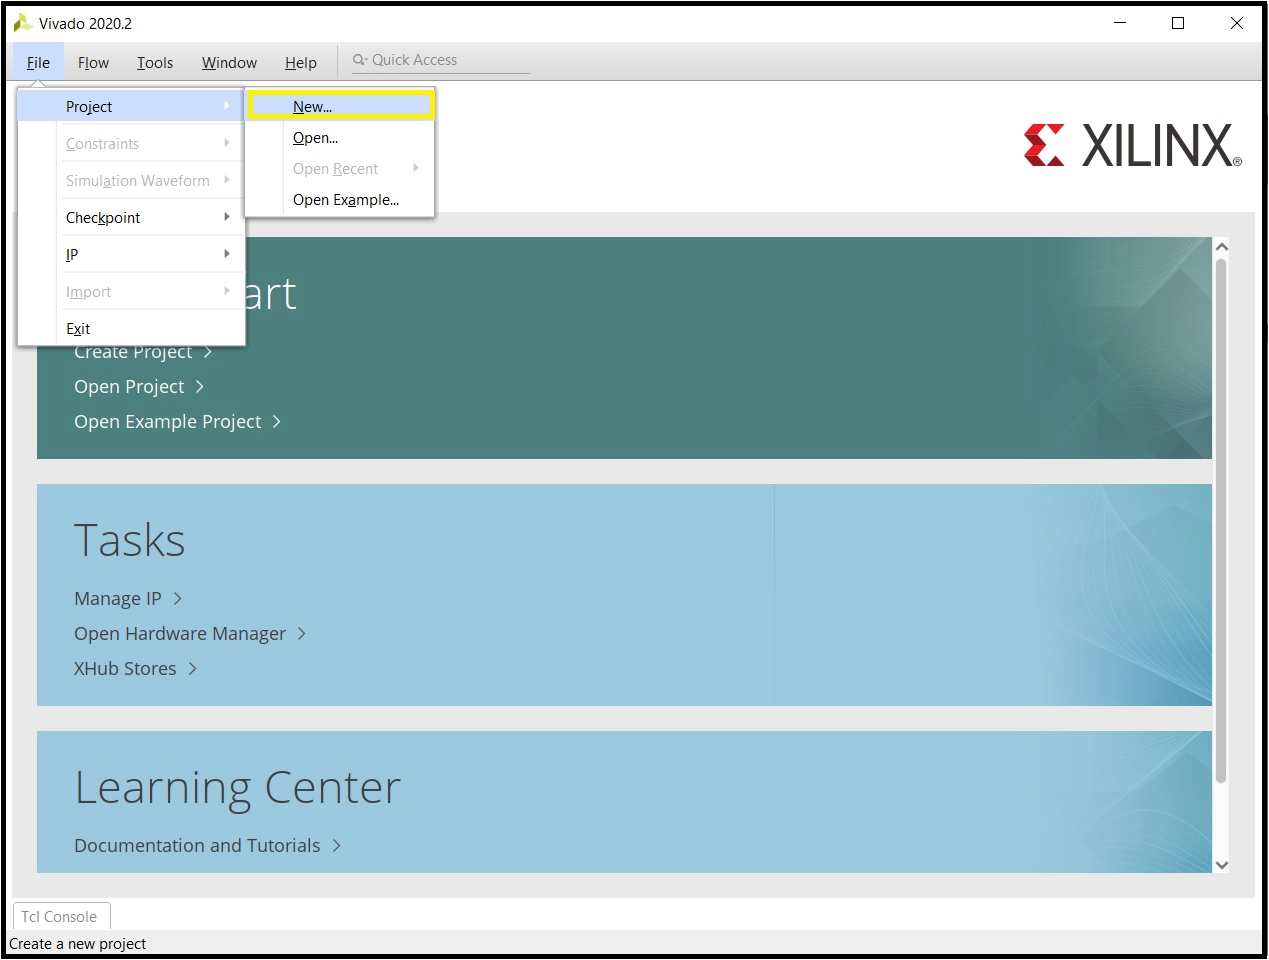
\includegraphics[width=\linewidth]{images/vivado01.png}
  \caption{Step 1: Open a project in VIVADO}
  \label{fig:vivado01}
\end{figure}

To access the Hardware Manager, open a project in VIVADO or create an empty one, if you do not have any projects yet.

\begin{figure}
  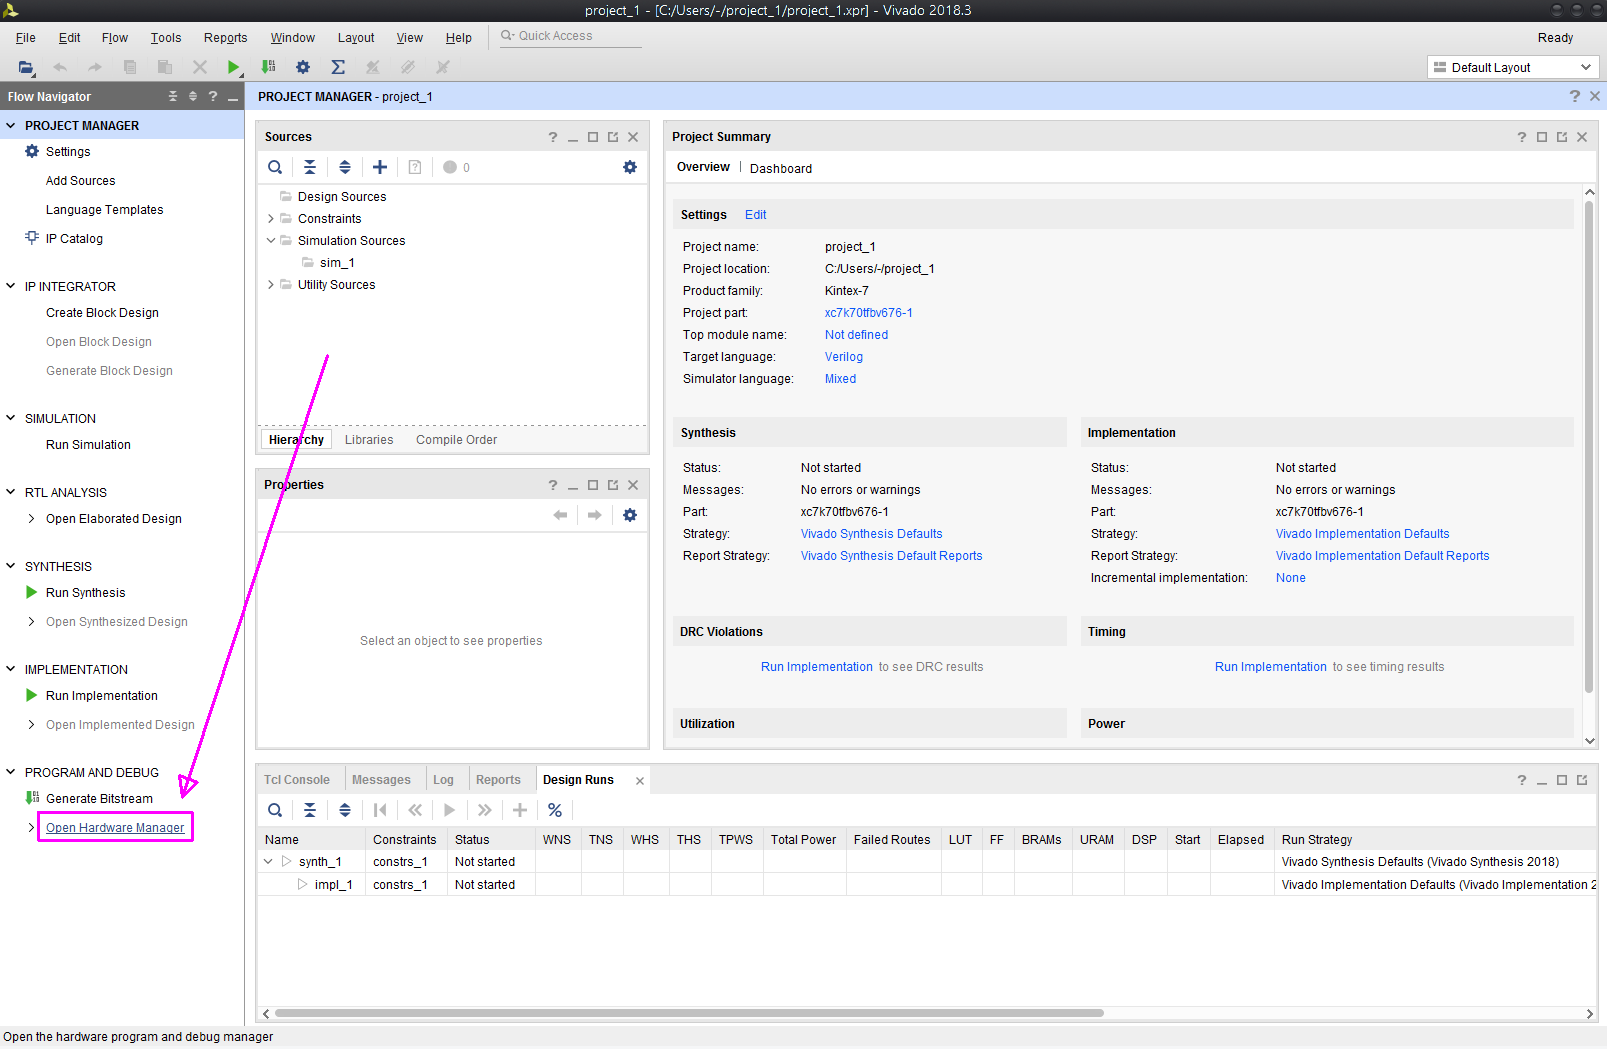
\includegraphics[width=\linewidth]{images/vivado02.png}
  \caption{Step 2: Open Hardware Manager}
  \label{fig:vivado02}
\end{figure}

In the left column, select "Open Hardware Manager" at the very bottom.

\begin{figure}
  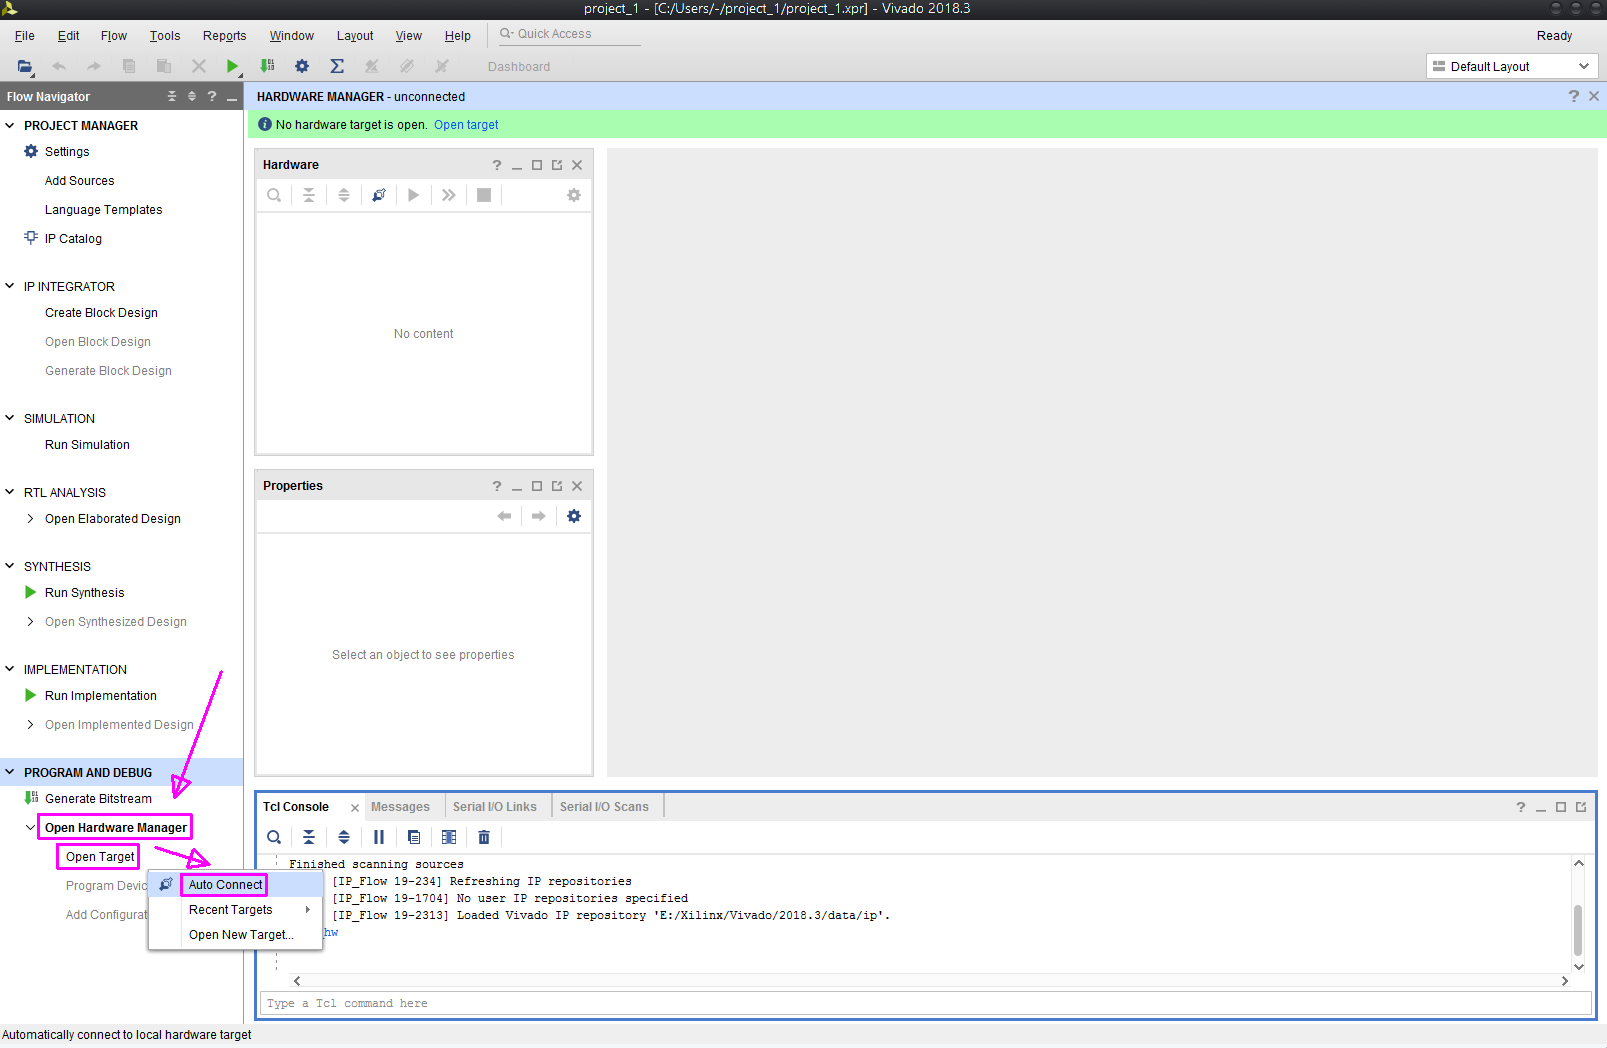
\includegraphics[width=\linewidth]{images/vivado03.png}
  \caption{Step 3: Connect to FPGA}
  \label{fig:vivado03}
\end{figure}

Under "Hardware Manager", choose "Open Target", then "Auto Connect".

\begin{figure}
  \includegraphics[width=\linewidth]{images/vivado04.png}
  \caption{Step 4: Wait a moment}
  \label{fig:vivado04}
\end{figure}

Wait a moment, "Connecting to server..."  should automatically close without dropping an error to the console.

\begin{figure}
  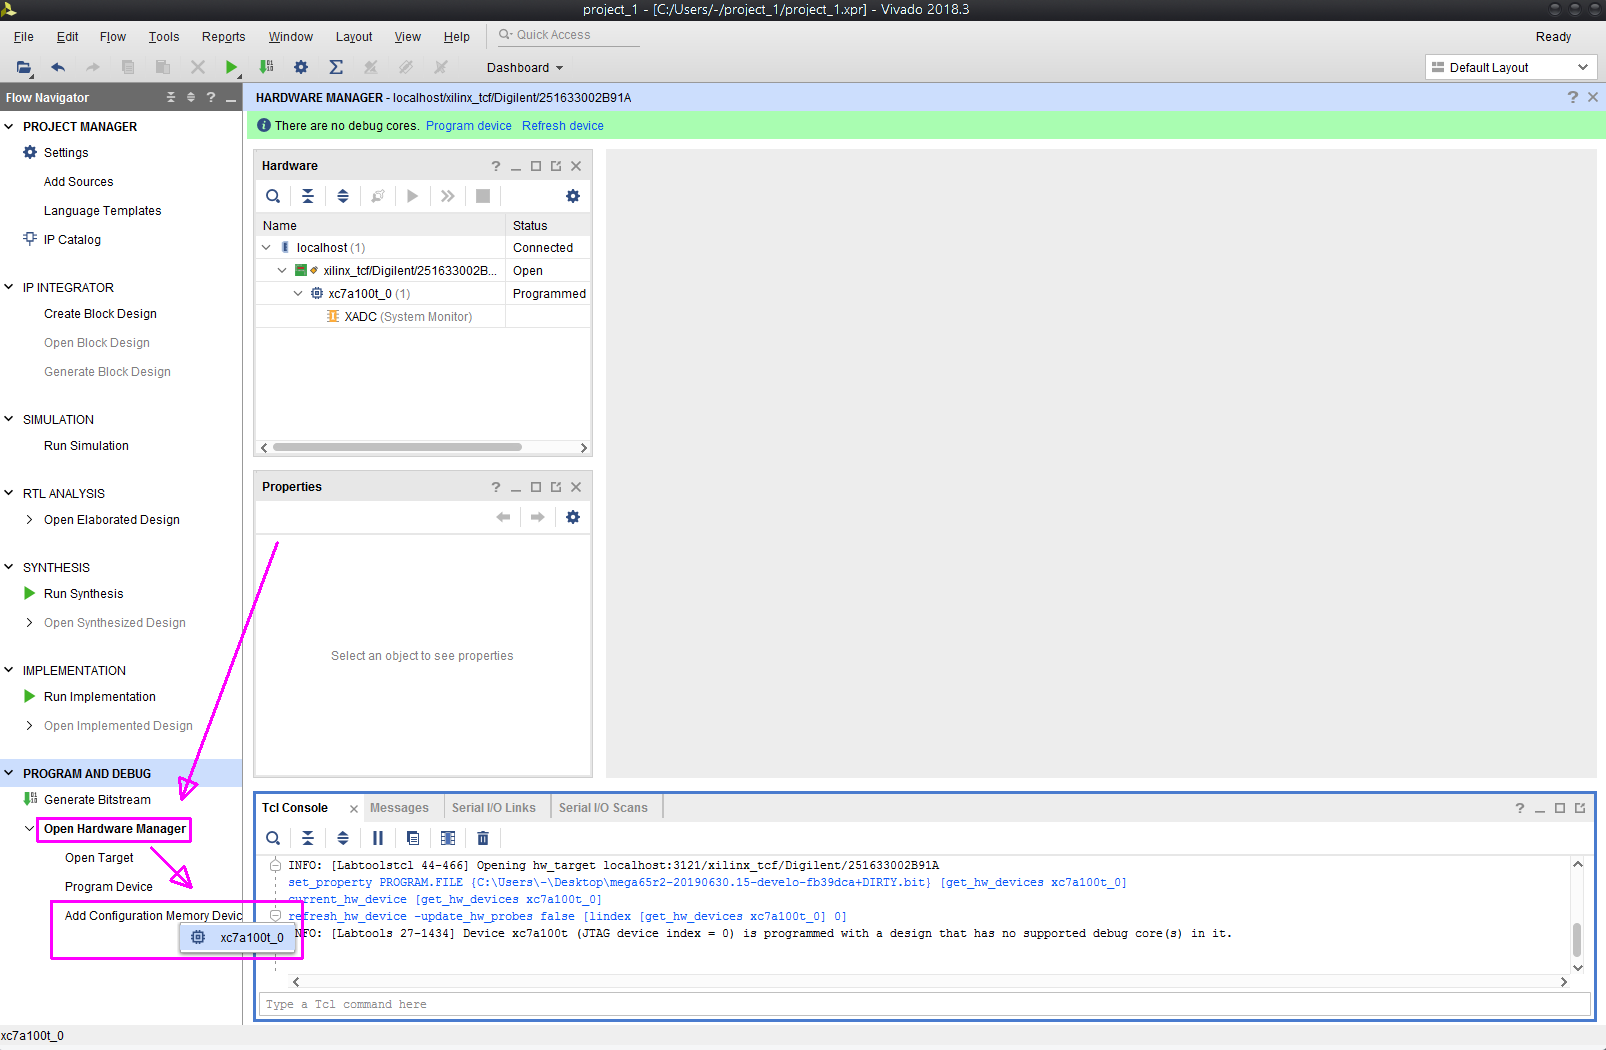
\includegraphics[width=\linewidth]{images/vivado05.png}
  \caption{Step 5: Add Configuration Memory Device}
  \label{fig:vivado05}
\end{figure}

Under "Hardware Manager", choose "Add Configuration Memory Device", then "xc7a100t_0".

\begin{figure}
  \includegraphics[width=\linewidth]{images/vivado06.png}
  \caption{Step 6: Select Memory Part}
  \label{fig:vivado06}
\end{figure}

In the newly opened dialogue, type "S25fl256s" (without quotes), then select "s25fl256sxxxxxxx0-spi-x1_x2_x4" (the upper one) and click "OK".

\begin{figure}
  \includegraphics[width=\linewidth]{images/vivado07.png}
  \caption{Step 7: Set programming options}
  \label{fig:vivado07}
\end{figure}

In the next dialogue, choose your local Configuration file, namely a bitstream with file suffix ".mcs". Leave all other parameters as they are (see /ref{fig:vivado07}).

\begin{figure}
  \includegraphics[width=\linewidth]{images/vivado08.png}
  \caption{Step 8: Programming in progress}
  \label{fig:vivado08}
\end{figure}

Patiently wait for the programming to finish, fingers crossed.

\begin{figure}
  \includegraphics[width=\linewidth]{images/vivado09.png}
  \caption{Step 9: Programming successful}
  \label{fig:vivado09}
\end{figure}

If your screen looks like /ref{fig:vivado09}, your new bistream has been successfully flashed into the Artix 100T FPGA!

\begin{figure}
  \includegraphics[width=\linewidth]{images/vivado09.png}
  \caption{Step 10: Reflashing the FPGA}
  \label{fig:vivado10}
\end{figure}

If you want to repeat the process, you might find the "Add Configuration Memory Device" option in step 5 greyed out. Instead, select "s25fl256sxxxxxxx0-spi-x1_x2_x4"  in the "Hardware" window, press right mouse button and select "Program Configuration Memory Device" to flash.

















  \chapter{Supporters \& Donors}

The MEGA65 would not have been possible to create without the generous support
of many organisations and individuals.

We are still compiling these lists, so apologies if we haven't included you yet.  If you
know anyone we have left out, please let us know, so that we can recognise the contribution
of everyone who has made the MEGA65 possible, and into the great retro-computing project
that it has become.

\section{Organisations}

\begin{itemize}
\item {\bf M.E.G.A. Museum of Electronic Games and Art, e.V., Germany} \megakey{Everything}
\item {\bf Trenz Electronik, Germany} \megakey{Motherboard}
\item {\bf Hintsteiner, Austria} \megakey{Case}
\item {\bf GMK, Germany} \megakey{Keyboard}
\end{itemize}

\section{Volunteers}

\begin{itemize}
\item Detlef Hastik \megakey{Founder} \megakey{Cat herding} \megakey{Testing} \megakey{Hosting}
\item Dr. Paul Gardner-Stephen \megakey{Founder} \megakey{VHDL} \megakey{Software}
\end{itemize}

\section{Contributors}

\setlength{\tabcolsep}{1mm}
\begin{tabular}{p{6cm}p{6cm}}

{\large\bf Andreas Liebeskind}     & {\large\bf Dr. Canan Hastik} \\
 \textit{(libi in paradize)}       & \textit{(indica)} \\
CFO MEGA eV                        & Chairwoman MEGA eV \\
& \\
{\large\bf Alexander Nik Petra}    & {\large\bf Wayne Johnson} \\
 \textit{(n0d)}                    &  \textit{(sausage)} \\
Early Case Design                  & Manual Additions \\
& \\
{\large\bf Ralph Egas}             & {\large\bf Lukas Kleiss} \\
 \textit{(0-limits)}               & \textit{(LAK132)} \\
Business Advisor                   & MegaWAT Presentation Software \\
& \\
{\large\bf Lucas Moss}             & {\large\bf Simon Jameson} \\
                                   & \textit{(Shallan)} \\
MEGAphone PCB Design               & Platform Enhancements \\
\end{tabular}

\section{Supporters}


% page 1
\newpage
\setlength{\tabcolsep}{1mm}
\begin{tabular}{p{4.5cm}p{4.5cm}p{4.5cm}}
@11110110100 & Anthony W. Leal & Carlos Silva \\
3c74ce64 & Arkadiusz Bronowicki & Carsten Sørensen \\
8-Bit Classics & Arkadiusz Kwasny & Cenk Miroglu Miroglu \\
Aaron Smith & Arnaud Léandre & Chang sik Park \\
Achim Mrotzek & Arne Drews & Charles A. Hutchins Jr. \\
Adolf Nefischer & Arne Neumann & Chris Guthrey \\
Adrian Esdaile & Arne Richard Tyarks & Chris Hooper \\
Adrien Guichard & Axel Klahr & Chris Stringer \\
Ahmed Kablaoui & Balaz Ondrej & Christian Boettcher \\
Alan Bastian Witkowski & Barry Thompson & Christian Eick \\
Alan Field & Benjamin Maas & Christian Gleinser \\
Alberto Mercuri & Bernard Alaiz & Christian Gräfe \\
Alexander Kaufmann & Bernhard Zorn & Christian Heffner \\
Alexander Niedermeier & Bieno Marti-Braitmaier & Christian Kersting \\
Alexander Soppart & Bigby & Christian Streck \\
Alfonso Ardire & Bill LaGrue & Christian Wyk \\
Amiga On The Lake & Bjoerg Stojalowski & Christoph Haug \\
Andre Kapp & Björn Johannesson & Christoph Huck \\
André Simeit & Bjørn Melbøe & Christoph Pross \\
André Wösten & Bo Goeran Kvamme & Christopher Christopher \\
Andrea Farolfi & Boerge Noest & Christopher Kalk \\
Andrea Minutello & Bolko Beutner & Christopher Kohlert \\
Andreas Behr & Brett Hallen & Christopher Nelson \\
Andreas Freier & Brian Gajewski & Christopher Taylor \\
Andreas Grabski & Brian Green & Christopher Whillock \\
Andreas Millinger & Brian Juul Nielsen & Claudio Piccinini \\
Andreas Nopper & Brian Reiter & Collen Blijenberg \\
Andreas Wendel Manufaktur & Bryan Pope & Constantine Lignos \\
Andreas Zschunke & Burkhard Franke & Crnjaninja \\
Andrew Bingham & Byron Goodman & Daniel Auger \\
Andrew Dixon & Carl Angervall & Daniel Julien \\
Andrew Mondt & Carl Danowski & Daniel Lobitz \\
Andrzej Hłuchyj & Carl Stock & Daniel O'Connor \\
Andrzej Sawiniec & Carl Wall & Daniel Teicher \\
Andrzej Śliwa & Carlo Pastore & Daniel Tootill \\
\end{tabular}
% page 2
\newpage
\setlength{\tabcolsep}{1mm}
\begin{tabular}{p{4.5cm}p{4.5cm}p{4.5cm}}
Daniel Wedin & EP Technical Services & Giampietro Albiero \\
Daniele Gaetano Capursi & Epic Sound & Giancarlo Valente \\
Dariusz Szczesniak & Erasmus Kuhlmann & Gianluca Girelli \\
David Asenjo Raposo & ergoGnomik & Giovanni Medina \\
David Dillard & Eric Hildebrandt & Glen Fraser \\
David Gorgon & Eric Hill & Glen R Perye III \\
David Norwood & Erwin Reichel & Glenn Main \\
David Raulo & Espen Skog & Gordon Rimac \\
David Ross & Evangelos Mpouras & GRANT BYERS \\
de voughn accooe & Ewan Curtis & Gregor Bubek \\
Dean Scully & Fabio Zanicotti & Gregor Gramlich \\
Dennis Jeschke & Fabrizio Di Dio & Guido Ling \\
Dennis Schaffers & Fabrizio Lodi & Guido von Gösseln \\
Dennis Schierholz & FARA Gießen GmbH & Guillaume Serge \\
Dennis Schneck & FeralChild & Gunnar Hemmerling \\
denti & First Choice Auto's & Günter Hummel \\
Dick van Ginkel & Florian Rienhardt & Gurce Isikyildiz \\
Diego Barzon & Forum64. de & Guy Simmons \\
Dierk Schneider & Francesco Baldassarri & Guybrush Threepwood \\
Dietmar Krueger & Frank Fechner & Hakan Blomqvist \\
Dietmar Schinnerl & Frank Haaland & Hans Pronk \\
Dirk Becker & Frank Hempel & Hans-Jörg Nett \\
Dirk Wouters & Frank Koschel & Harald Dosch \\
Domingo Fivoli & Frank Linhares & Harri Salokorpi \\
DonChaos & Frank Wolf & Harry Culpan \\
Donn Lasher & FranticFreddie & Heath Gallimore \\
Douglas Johnson & Fredrik Ramsberg & Heinz Roesner \\
Dr. Leopold Winter & Fridun Nazaradeh & Heinz Stampfli \\
Dusan Sobotka & Friedel Kropp & Helge Förster \\
Earl Woodman & Garrick West & Hendrik Fensch \\
Ed Reilly & Gary Lake-Schaal & Henning Harperath \\
Edoardo Auteri & Gary Pearson & Henri Parfait \\
Eduardo Gallardo & Gavin Jones & Henrik Kühn \\
Eduardo Luis Arana & Geir Sigmund Straume & Holger Burmester \\
Eirik Juliussen Olsen & Gerd Mitlaender & Holger Sturk \\
\end{tabular}
% page 3
\newpage
\setlength{\tabcolsep}{1mm}
\begin{tabular}{p{4.5cm}p{4.5cm}p{4.5cm}}
Howard Knibbs & Jeffrey van der Schilden & Kai Pernau \\
Hubert de Hollain & Jens Schneider & Kalle Pöyhönen \\
Huberto Kusters & Jens-Uwe Wessling & Karl-Heinz Blum \\
Hugo Maria Gerardus v.d. Aa & Jesse DiSimone & Karsten Engstler \\
Humberto Castaneda & Johan Arneklev & Karsten Westebbe \\
Ian Cross & Johan Svensson & Kenneth Dyke \\
IDE64 Staff & Johannes Fitz & Kenneth Joensson \\
Igor Ianov & John Cook & Kevin Edwards \\
Immo Beutler & John Deane & Kevin Thomasson \\
Ingo Keck & John Nagi & Kim Jorgensen \\
Insanely Interested Publishing & John Rorland & Kim Rene Jensen \\
IT-Dienstleistungen Obsieger & John Sargeant & Kimmo Hamalainen \\
Ivan Elwood & John Traeholt & Konrad Buryło \\
Jaap HUIJSMAN & Jon Sandelin & Kosmas Einbrodt \\
Jace Courville & Jonas Bernemann & Kurt Klemm \\
Jack Wattenhofer & Jonathan Prosise & Lachlan Glaskin \\
Jakob Schönpflug & Joost Honig & Large bits collider \\
Jakub Tyszko & Jordi Pakey-Rodriguez & Lars Becker \\
James Hart & Jöre Weber & Lars Berntsson \\
James McClanahan & Jörg Jungermann & Lars Edelmann \\
James Sutcliffe & Jörg Schaeffer & Lars Slivsgaard \\
Jan Bitruff & Jörg Weese & Lasse Lambrecht \\
Jan Hildebrandt & Josef Hesse & Lau Olivier \\
Jan Iemhoff & Josef Soucek & Lee Chatt \\
Jan Kösters & Josef Stohwasser & Loan Leray \\
Jan Peter Borsje & Joseph Gerth & Lorenzo Quadri \\
Jan Schulze & Jovan Crnjanin & Lorenzo Travagli \\
Jan Stoltenberg-Lerche & Juan Pablo Schisano & Lorin Millsap \\
Janne Tompuri & Juan S. Cardona Iguina & Lothar Serra Mari \\
Jannis Schulte & JudgeBeeb & Luca Papinutti \\
Jari Loukasmäki & Juliussen Olsen & Ludek Smetana \\
Jarrod Adams & Juna Luis Fernandez Garcia & Lukas Burger \\
Jason Smith & Jürgen Endras & Lutz-Peter Buchholz \\
Javier Gonzalez Gonzalez & Jürgen Herm Stapelberg & Luuk Spaetgens \\
Jean-Paul Lauque & Jyrki Laurila & Mad Web Skills \\
\end{tabular}
% page 4
\newpage
\setlength{\tabcolsep}{1mm}
\begin{tabular}{p{4.5cm}p{4.5cm}p{4.5cm}}
MaDCz & Markus Dauberschmidt & Max Ihlenfeldt \\
Magnus Wiklander & Markus Fehr & Meeso Kim \\
Maik Diekmann & Markus Fuchs & Michael Dailly \\
Malte Mundt & Markus Guenther-Hirn & Michael Dötsch \\
Manuel Beckmann & Markus Liukka & Michael Dreßel \\
Manzano Mérida & Markus Roesgen & Michael Fichtner \\
Marc "3D-vice" Schmitt & Markus Uttenweiler & Michael Fong \\
Marc Bartel & Martin Bauhuber & Michael Geoffrey Stone \\
Marc Jensen & Martin Benke & Michael Gertner \\
Marc Theunissen & Martin Gendera & Michael Grün \\
Marc Tutor & Martin Groß & Michael Habel \\
Marc Wink & Martin Gutenbrunner & Michael Härtig \\
Marcel Buchtmann & Martin Johansen & Michael Haynes \\
Marcel Kante & Martin Marbach & Michael J Burkett \\
Marco Beckers & Martin Sonnleitner & Michael Jensen \\
Marco Cappellari & Martin Steffen & Michael Jurisch \\
Marco Rivela & Marvin Hardy & Michael Kappelgaard \\
Marco van de Water & Massimo Villani & Michael Kleinschmidt \\
Marcus Gerards & Mathias Dellacherie & Michael Lorenz \\
Marcus Herbert & Mathieu Chouinard & Michael Mayerhofer \\
Marcus Linkert & Matthew Adams & Michael Nurney \\
Marek Pernicky & Matthew Carnevale & Michael Rasmussen \\
Mario Esposito & Matthew Palmer & Michael Richmond \\
Mario Fetka & Matthew Santos & Michael Sachse \\
Mario Teschke & Matthias Barthel & Michael Sarbak \\
Mariusz Tymków & Matthias Dolenc & Michael Scholz \\
Mark Adams & Matthias Fischer & Michael Timm \\
Mark Green & Matthias Frey & Michael Traynor \\
Mark Hucker & Matthias Grandis & Michal Ursiny \\
Mark Leitiger & Matthias Guth & Michele Chiti \\
Mark Spezzano & Matthias Lampe & Michele Perini \\
Mark Watkin & Matthias Meier & Michele Porcu \\
Marko Rizvic & Matthias Mueller & Miguel Angel Rodriguez Jodar \\
Markus Bieler & Matthias Nofer & Mikael Lund \\
Markus Bonet & Matthias Schonder & Mike Betz \\
\end{tabular}
% page 5
\newpage
\setlength{\tabcolsep}{1mm}
\begin{tabular}{p{4.5cm}p{4.5cm}p{4.5cm}}
Mike Kastrantas & Patrick Vogt & Ralf Smolarek \\
Mike Pikowski & Paul Alexander Warren & Ralf Zenker \\
Mikko Hämäläinen & Paul Jackson & Ralph Bauer \\
Mikko Suontausta & Paul Johnson & Ralph Wernecke \\
Mirko Roller & Paul Massay & Rédl Károly \\
Miroslav Karkus & Paul Westlake & Reiner Lanowski \\
Morgan Antonsson & Paul Woegerer & Remi Veilleux \\
Moritz & Pauline Brasch & Riccardo Bianchi \\
Morten Nielsen & Paulo Apolonia & Richard Englert \\
MUBIQUO APPS,SL & Pete Collin & Richard Good \\
Myles Cameron-Smith & Peter Eliades & Richard Menedetter \\
Nelson & Peter Gries & Richard Sopuch \\
neoman & Peter Habura & Rick Reynolds \\
Nicholas Melnick & Peter Herklotz & Rico Gruninger \\
Nikolaj Brinch Jørgensen & Peter Huyoff & Rob Dean \\
Nils Andreas & Peter Leswell & Robert Bernardo \\
Nils Eilers & Peter Weile & Robert Eaglestone \\
Nils Hammerich & Petri Alvinen & Robert Grasböck \\
Nils77 & Philip Marien & Robert Miles \\
Norah Smith & Philip Timmermann & Robert Schwan \\
Norman King & Philipp Rudin & Robert Shively \\
Olaf Grunert & Pierre Kressmann & Robert Tangmar \\
Ole Eitels & Pieter Labie & Robert Trangmar \\
Oliver Boerner & Piotr Kmiecik & Rodney Xerri \\
Oliver Brüggmann & Power-on.at & Roger Olsen \\
Oliver Smith & Przemysław Safonow & Roger Pugh \\
Olivier Bori & Que Labs & Roland Attila Kett \\
ONEPSI LLC & R Welbourn & Roland Evers \\
oRdYNe & R-Flux & Roland Schatz \\
Osaühing Trioflex & Rafał Michno & Rolf Hass \\
Padawer & Rainer Kappler & Ronald Cooper \\
Patrick Becher & Rainer Weninger & Ronald Hunn \\
Patrick Bürckstümmer & Ralf Griewel & Ronny Preiß \\
Patrick de Zoete & Ralf Reinhardt & Roy van Zundert \\
Patrick Toal & Ralf Schenden & Rüdiger Wohlfromm \\
\end{tabular}
% page 6
\newpage
\setlength{\tabcolsep}{1mm}
\begin{tabular}{p{4.5cm}p{4.5cm}p{4.5cm}}
Ruediger Schlenter & Steve Gray & Tim Krome \\
Russell Peake & Steve Kurlin & Tim Waite \\
Rutger WIllemsen & Steve Lemieux & Timo Weirich \\
Sampo Peltonen & Steven Combs & Timothy Blanks \\
Sarmad Gilani & Stewart Dunn & Timothy Henson \\
SAS74 & Stuart Marsh & Timothy Prater \\
Scott Halman & Sven Neumann & Tobias Butter \\
Scott Hollier & Sven Stache & Tobias Heim \\
Scott Robison & Sven Sternberger & Tobias Köck \\
Sebastian Baranski & Szabolcs Bence & Tobias Lüthi \\
Sebastian Bölling & Tantrumedia Limited & Toni Ammer \\
Sebastian Felzmann & Techvana Operations Ltd. & Tore Olsen \\
Sebastian Lipp & Teddy Turmeaux & Torleif Strand \\
Sebastian Rakel & Teemu Korvenpää & Torsten Schröder \\
Şemseddin Moldibi & The Games Foundation & Tuan Nguyen \\
Seth Morabito & Thierry Supplisson & Uffe Jakobsen \\
Shawn McKee & Thieu-Duy Thai & Ulrich Hintermeier \\
Siegfried Hartmann & Thomas Bierschenk & Ulrich Nieland \\
Sigurbjorn Larusson & Thomas Edmister & Ulrik Kruse \\
Sigurdur Finnsson & Thomas Frauenknecht & Ursula Förstle \\
Simon Lawrence & Thomas Gitzen & Uwe Boschanski \\
Simon Wolf & Thomas Gruber & Vedran Vrbanc \\
spreen.digital & Thomas Haidler & Verm Project \\
Stefan Haberl & Thomas Jager & Wayne Sander \\
Stefan Kramperth & Thomas Karlsen & Wayne Steele \\
Stefan Richter & Thomas Laskowski & Who Knows \\
Stefan Sonnek & Thomas Marschall & Winfried Falkenhahn \\
Stefan Theil & Thomas Niemann & Wolfgang Becker \\
Stefan Vrampe & Thomas Scheelen & Wolfgang Stabla \\
Stefano Canali & Thomas Schilling & Worblehat \\
Stefano Mozzi & Thomas Tahsin-Bey & www.patop69.net \\
Steffen Reiersen & Thomas Walter & Yan B \\
Stephan Bielmann & Thomas Wirtzmann & Zoltan Markus \\
Stephen Jones & Thorsten Knoll & Zytex Online Store \\
\end{tabular}

\end{appendices}


\nocite{*}
\bibliographystyle{IEEEtran}
\bibliography{references}

\printindex

%
% The element catalogue holds tests of components, macros, fonts, or any element for the
% use of displaying as a test, or an example of how to use.
%
% When outputting a production version of the User Guide, this file should not be included.
%


\part{ELEMENT CATALOGUE}

\section{Graphic Symbols Font}

Graphic chars and MEGA logo using the {\bf graphicsymbol} macro:

\graphicsymbol{`\textcolor{red}{`} qQwWUcbdhjIJK \textcolor{blue}{`}`}

Graphic chars using the {\bf symbolfont} font definition:

\begin{symbolfont}%
	qQwWeErRtTyYuUiIoOpP\\
	aAsSdDfFgGhHjJkKlL\\
	zZxXcCvVbBnNmM%
\end{symbolfont}%

The MEGA logo in default black using the {\bf megasymbol} macro:

\megasymbol for tables and symbol usage.

The MEGA logo using a passed in colour:

\megasymbol[black]
\megasymbol[brown]
\megasymbol[orange]
\megasymbol[blue]

Special multi-line keys:
\specialkey{RUN STOP}%
\specialkey{CLR HOME}%
\specialkey{NO SCROLL}%
\specialkey{HELP}%
\specialkey{INST DEL}%
\specialkey{SHIFT LOCK}%
\specialkey{ESC}%
\specialkey{ALT}

\section{Handy Symbols}
Registered symbol for companies, for example: Amiga\textregistered \ is \begin{verbatim}
\textregistered
\end{verbatim}

Trademark symbol for companies, for example: Commodore 64\texttrademark{} is \begin{verbatim}
\texttrademark{}
\end{verbatim}

Amiga\texttrademark{} computers

\section{Keyboard keys}

\megasymbolkey MEGA key looks like this.

\megakey{Normal Shift}\\
\megakey[title]{Big Shift}

Text to the left \specialkey{RUN STOP} and text to the right.

\specialkey{SHIFT} \specialkey{CTRL} \megakey{9}  \megakey{ } \specialkey{RETURN}

\megakey{*} \megakey{$\leftarrow$} \megakey{$\uparrow$} \megakey{$\rightarrow$} \megakey{$\downarrow$}

\section{Screen Output}

\begin{screenoutput}
	10 INPUT A$
	20 PRINT "YOU TYPED: ";A$
	30 PRINT
	40 GOTO 10
	RUN
	? MEGA 65
	YOU TYPED: MEGA 65
\end{screenoutput}

\begin{screenoutput}
10 OPEN 1,8,0,"$0:*,P,R
20 : IF DS THEN PRINT DS$: GOTO 100
30 GET#1,X$,X$
40 DO
50 : GET#1,X$,X$: IF ST THEN EXIT
60 : GET#1,BL$,BH$
70 : LINE INPUT#1, F$
80 : PRINT LEFT$(F$,18)
90 LOOP
100 CLOSE 1

RUN
\end{screenoutput}

Use the "screentext" macro to perform 80 column inline screen text:
\screentext{?SYNTAX ERROR}

Use the "screentext" macro to perform 40 column inline screen text:
\screentextwide{?SYNTAX ERROR}

\section{Screen font mapping}


\begin{minipage}{5cm}
\verbatimfont{\codefont}
\begin{verbatim}
0123456789ABCDEF  UTF8
----------------------
 !"#$%&'()*+,-./    20
0123456789:;<=>?    30
@ABCDEFGHIJKLMNO    40
PQRSTUVWXYZ[\]^_    50
`abcdefghijklmno    60
pqrstuvwxyz{|}~     70

ÀÁÂÃÄÅÆÇÈÉÊËÌÍÎÏ  c380
ÐÑÒÓÔÕÖ×ØÙÚÛÜÝÞß  c390
àáâãäåæçèéêëìíîï  c3a0
ðñòóôõö÷øùúûüýþÿ  c3b0

ĀāĂ㥹ĆćĈĉĊċČčĎď  c480
ĐđĒēĔĕĖėĘęĚěĜĝĞğ  c490
ĠġĢģĤĥĦħĨĩĪīĬĭĮį  c4a0
İıIJijĴĵĶķĸĹĺĻļĽľĿ  c4b0

ŀŁłŃńŅņŇňʼnŊŋŌōŎŏ  c580
ŐőŒœŔŕŖŗŘřŚśŜŝŞş  c590
ŠšŢţŤťŦŧŨũŪūŬŭŮů  c5a0
ŰűŲųŴŵŶŷŸŹźŻżŽžſ  c5b0
ƀƁƂƃƄƅƆƇƈƉƊƋƌƍƎƏ  c680
ƐƑƒƓƔƕƖƗƘƙƚƛƜƝƞƟ  c690

ƠơƢƣƤƥƦƧƨƩƪƫƬƭƮƯ  c6a0
ưƱƲƳƴƵƶƷƸƹƺƻƼƽƾƿ  c6b0
ǀǁǂǃDŽDždžLJLjljNJNjnjǍǎǏ  c780
ǐǑǒǓǔǕǖǗǘǙǚǛǜǝǞǟ  c790
\end{verbatim}
\end{minipage}
\begin{minipage}{5cm}
\verbatimfont{\ttfamily}
\begin{verbatim}
0123456789ABCDEF  UTF8
----------------------
 !"#$%&'()*+,-./    20
0123456789:;<=>?    30
@ABCDEFGHIJKLMNO    40
PQRSTUVWXYZ[\]^_    50
`abcdefghijklmno    60
pqrstuvwxyz{|}~     70

ÀÁÂÃÄÅÆÇÈÉÊËÌÍÎÏ  c380
ÐÑÒÓÔÕÖ×ØÙÚÛÜÝÞß  c390
àáâãäåæçèéêëìíîï  c3a0
ðñòóôõö÷øùúûüýþÿ  c3b0

ĀāĂ㥹ĆćĈĉĊċČčĎď  c480
ĐđĒēĔĕĖėĘęĚěĜĝĞğ  c490
ĠġĢģĤĥĦħĨĩĪīĬĭĮį  c4a0
İı  ĴĵĶķ ĹĺĻļĽľĿ  c4b0
ŀŁłŃńŅņŇň ŊŋŌōŎŏ  c580
ŐőŒœŔŕŖŗŘřŚśŜŝŞş  c590

ŠšŢţŤť  ŨũŪūŬŭŮů  c5a0
ŰűŲųŴŵŶŷŸŹźŻżŽžſ  c5b0
                  c680
                  c690

                  c6a0
                  c6b0
             ǍǎǏ  c780
ǐǑǒǓǔǕǖǗǘǙǚǛǜǝǞǟ  c790
\end{verbatim}
\end{minipage}

\section{Sprite Grids}
\subsection{Balloon Sprite Demo}

\spritegrid{
  \hline
  \spritecells{---------ooooo----------}
  \spritecells{-------ooooooooo--------}
  \spritecells{------ooooooooooo-------}
  \spritecells{------ooo--o---oo-------}
  \spritecells{-----ooo-ooo-ooooo------}
  \spritecells{-----ooo-ooo-ooooo------}
  \spritecells{-----ooo---o---ooo------}
  \spritecells{-----ooo-o-ooo-ooo------}
  \spritecells{-----ooo-o-ooo-ooo------}
  \spritecells{-----ooo---o--oooo------}
  \spritecells{------ooooooooooo-------}
  \spritecells{------ooooooooooo-------}
  \spritecells{-------ooooooooo--------}
  \spritecells{-------o-ooooo-o--------}
  \spritecells{--------o-o-o-o---------}
  \spritecells{--------o--o--o---------}
  \spritecells{---------o-o-o----------}
  \spritecells{---------o-o-o----------}
  \spritecells{---------ooooo----------}
  \spritecells{---------ooooo----------}
  \spritecells{----------ooo-----------}
}

\newpage

\subsection{Multi-Colour Sprite}

\spritegrid{
  \hline
  \spritecells{------------------------}
  \spritecells{------------------------}
  \spritecells{------------------------}
  \spritecells{------------------------}
  \spritecells{llllllllllllllllllllllll}
  \spritecells{llllllllllllllllllllllll}
  \spritecells{lllllleeeeeelleeeeeeeell}
  \spritecells{lllloooooooollooooooooll}
  \spritecells{llllooggggggllooggggggll}
  \spritecells{lllloolllllllloollllllll}
  \spritecells{llllooeeeellllooeeeellll}
  \spritecells{lllloooooooollooooooooll}
  \spritecells{llllooggggoollggggggooll}
  \spritecells{lllloolllloollllllllooll}
  \spritecells{llllooeeeeoolleeeeeeooll}
  \spritecells{llllggooooggllooooooggll}
  \spritecells{llllllggggllllggggggllll}
  \spritecells{llllllllllllllllllllllll}
  \spritecells{------------------------}
  \spritecells{------------------------}
  \spritecells{------------------------}
}


\input{common-footer}

